\documentclass[10pt,a4paper,twoside]{book}
\usepackage[utf8]{inputenc}
\usepackage[english]{babel}
\usepackage[titletoc]{appendix}
\usepackage[vscale=0.8,left=3cm,right=2cm,footskip=2.5cm, headsep=1cm]{geometry}
\usepackage{amsmath, amsfonts, amssymb, graphicx}
\usepackage[pdfborder={0 0 0 }]{hyperref}
\usepackage{enumerate, enumitem, color, rotating, subfig, placeins, dsfont, listliketab, dirtree} 
\usepackage{titlesec}
\usepackage{url}
\usepackage{pdflscape}
\usepackage{rotating}

\pdfminorversion=5

\newcommand{\OP}[1]{{\bf\widehat{#1}}}
\newcommand{\ket}[1]{\left| #1 \right>}
\newcommand{\bra}[1]{\left< #1 \right|}
\newcommand{\braket}[2]{\left\langle #1 | #2\right\rangle}
\newcommand{\I}{\mathds{1}}
\newcommand{\x}{\otimes}
\newcommand{\su}{\uparrow}
\newcommand{\sd}{\downarrow}	
\newcommand{\ph}{\phi(\mathbf{r}, t)}
\newcommand{\Ph}{\Phi(\mathbf{r}, t)}
\newcommand{\Phn}{\Phi(\mathbf{r}, t_0)}
\newcommand{\PT}{\Psi_T(\mathbf{r})}
\newcommand{\Ptau}{\Phi(\mathbf{r}, \tau)}
\newcommand{\mbf}[1]{\mathbf{#1}}

\newcommand{\Var}{\mathrm{Var}}
\newcommand{\Exp}[1]{\left< #1 \right>}
\newcommand{\Cov}{\mathrm{Cov}}


\newcommand{\subfigure}{\subfloat}


\usepackage{listings}

% Code parameters
\lstset{language=c++}
\lstset{basicstyle=\ttfamily\footnotesize}
\lstset{backgroundcolor=\color{grey}}
\lstset{stringstyle=\color{beige}}
\lstset{keywordstyle=\color{green}\bfseries}
\lstset{commentstyle=\color{red}}
\lstset{showspaces=false}
\lstset{showstringspaces=false}
\lstset{showtabs=false}
\lstset{breaklines}
\lstset{numbers=left, numberstyle=\tiny, stepnumber=1, numbersep=5pt}
\lstset{linewidth=16cm}

\setlength{\parskip}{11pt}
\setlength{\parindent}{0mm}

\definecolor{grey}{rgb}{0.92,0.92,0.92}
\definecolor{green}{rgb}{0, 0.4, 0}
\definecolor{beige}{rgb}{0.62, 0.44, 0.1}


\titleformat{\section}
{\normalfont\Large\bfseries}
{\color{green}\thesection}{1em}{\underline}

\titleformat{\subsection}
{\normalfont\large\bfseries}
{\color{green}\thesubsection}{1em}{}

\titleformat{\chapter}[frame]
{\normalfont\Huge\bfseries}
{\color{black}\hspace{0.5cm}\thechapter\hspace{0.5cm}}{1em}{\color{green}}

% \setlength{\fboxrule}{0.5mm}
\newcommand{\cfbox}[2]{%
    \color{green}%
    \addtolength{\linewidth}{-2\fboxsep}%
    \addtolength{\linewidth}{-2\fboxrule}%

    \fbox{%
      \color{black}%
        \begin{minipage}{#1 + \linewidth}
	  #2
	\end{minipage}
    }
    \color{black}
}

\begin{document}
\begin{titlepage}
\begin{center}
\ \\
\ \\
\ \\
{\huge \bf Quantum Monte-Carlo studies of generalized systems of many particles}\\ 
\ \\ 
{\Large by}\\
\ \\
{\Large \bf J\o{}rgen H\o{}gberget}\\
\ \\
\ \\
\ \\
\ \\
{\large \bf THESIS}\\
{\large for the degree of}\\
{\large \bf MASTER OF SCIENCE}\\
\ \\
(Master in Computational Physics)\\
\ \\
\ \\
\begin{figure}[h!]
\begin{center}

\includegraphics[width=0.3\textwidth]{../Graphics/uiologo.pdf}
\end{center}
\end{figure}
\ \\
\Large{\rm Faculty of Mathematics and Natural Sciences}\\
{\rm Department of Physics}\\
{\rm University of Oslo}\\
\ \\
\ \\
{\rm June 2013}
\end{center}
\end{titlepage}

\chapter*{Preface}

blah blah
\tableofcontents
\chapter{Introduction}

Studies of general systems demand a general solver. The process of developing code aimed at a specific task is fundamentally different from the process of developing a general solver, simply due to the fact that the general equations need to be implemented \textit{independent} of any specific properties a modelled system may contain. This is most commonly achieved through object oriented programming, which allows for the code to be structured into general implementations and specific implementations. The general - and specific implementations can then be interfaced through a functionality referred to as \textit{polymorphism}. The aim of this thesis is to use object oriented C++ to build a general and efficient Quantum Monte-Carlo (QMC) solver, which can tackle several many-body systems, from confined electron systems, i.e. quantum dots, to bosons.  

A constraint put on the QMC solver in this thesis is that the ansatz for the \textit{trial wave function} consists of a single term, i.e. a single \textit{Slater determinant}. This opens up the possibility to study systems consisting of a large number of particles, due to efficient optimizations in the single determinant. A simple trial wave function will also  significantly ease the implementation of different systems, and thus make it easier to develop a general framework within the given time frame.

Given the simple ansatz for the wave function, the precision of Variational Monte-Carlo (VMC) is expected to be far from optimal, however, Diffusion Monte-Carlo (DMC) is supposed to withstand this problem, and thus yield a good final estimate nevertheless. To study this purposed power of DMC is another main focus of this thesis, in addition to pushing the limits regarding optimization of the code, and thus run ab-initio simulations of a large number of particles.

The two-dimensional quantum dot was chosen as the system of reference around which the code was planned. The reason for this is that all the current Master students are studying quantum dots at some level, which means that we can help each other reach a collective understanding of the system. Additionally, Sarah Reimann has studied two-dimensional quantum dots for up to 56 particles using a non-variational method called \textit{Similarity Renormalization Group theory} \cite{verdensBesteArtikkel}. Providing her with precise variational DMC benchmarks were considered to be of utmost importance. Coupled Cluster Singles and Doubles (CCSD) results are done up to 56 particles by Christoffer Hirth \cite{Hirth}, however, for the lower frequencies, i.e. for higher correlations, CCSD struggles with convergence.   

Depending on the success of the implementation, various additional systems could be implemented and studied in detail, such as atomic systems, three-dimensional - and double-well quantum dots. 

Apart from benchmarking DMC ground state energies, the specific aim in the case of quantum dots is to study their behavior as the frequency is lowered. A lower frequency implies a higher correlation in the system. Understanding these correlated systems of electrons are of great importance to many-body theory in general. The effect of adding a third dimension is also of high interest. The advantage of DMC compared to other methods is that the distribution is relatively easy to obtain.

Ground state energies for atomic systems can be benchmarked against experimental results \cite{H_He_exact, ExactMolecules, AtomsExact, KryptonExact}, that is, precise calculations which are believed to be very close to the exact result for the given Hamiltonian, which yields an excellent opportunity to test the limits of DMC given a simple trial wave function. Going further to molecular systems, an additional aim is to explore the transition between QMC and molecular dynamics by parameterizing simple force field potentials \cite{forcesQMC}.

Several former Master students, such as Christoffer Hirth \cite{Hirth} and Veronica K.B. Olsen \cite{Olsen}, have studied two-dimensional quantum dots in the past, and have thus generated ground state energies to  which the DMC energies can be compared. For three-dimensional quantum dots, few results are available for benchmarking.

\subsubsection{The structure of the thesis}

\begin{itemize}
 \item The first chapter introduces the concept of object oriented programming, with focus on the methods used to develop the code for this thesis. The reader is assumed to have some background in programming, hence the very fundamentals of programming are not presented. A full documentation of the code is available in Ref. \cite{libBorealisCode}. The code will thus not be covered in full detail. In addition to concepts from C++ programming, Python scripting will be introduced. General strategies regarding planning and structuring of code will also be covered in detail. The two most important Python scripts used in this thesis are documented in Appendix \ref{appendix:sympy} and Appendix \ref{appendix:DCVIZ}.
 
 \item The second chapter serves as a theoretical introduction to QMC, discussing the necessary many-body theory in detail. Important theory which is required to understand the concepts introduced in later chapters are given the primary focus. The reader is assumed to have a basic understanding of Quantum Wave Mechanics. An introduction to the commonly used Dirac notation is given in Appendix \ref{app:Dirac}.
 
 \item Chapter \ref{ch:optAndGen} presents all the assumptions regarding the systems modelled in this thesis together with the aims regarding the generalization and optimization of the code. The strategies applied to achieve these aims will then be covered in high detail.
 
 \item Chapter \ref{ch:modelledSystems} introduces the systems modelled in this thesis, that is, the quantum dots and atomic systems. The single particle wave functions used to generate the trial wave functions for the different systems are presented together with the respective Hamiltonians.
 
 \item The results, along with the discussions and the conclusions mark the final part of this thesis. Results for up to 56 electrons in the two-dimensional quantum dot are presented and comparisons are made with two - and three-dimensional quantum dots for high and low frequency ranges. A brief display of a double-well quantum dot is then given before the atomic results are presented. The ground state energies of atoms up to Krypton and molecules up to $\mathrm{O_2}$ are then compared to experimental values. Concluding the results section, the molecular energies as a function of the separation of cores are compared to the Lennard-Jones 12-6 potential \cite{MD1, MD2}. Final remarks are then made regarding further work expanding on the work done in this thesis. 
\end{itemize}
\part{Theory}
\chapter{Scientific Programming}

The introduction of the computer around World War II had a major impact on the mathematical fields of science. Previously unsolvable problems were now  solvable. The question was no longer whether or not it was possible, but rather to what precision and with which method. The computer spawned a new branch of physics, \textit{computational physics}, breaching barriers no one could even imagine existed. The first major result of this synergy between science and computers came with the infamous atomic bombs \textit{Little Boy} and \textit{Fat Man}, a product of \textit{The Manhattan Project} leaded by \textit{J. Robert Oppenheimer} \cite{supermen}.

\section{Programming Languages}

Writing a program, or a code, is a list of instructions for the computer. It is in many ways similar to writing human-to-human instructions. You may use different programming languages, such as C++, Python, Java, as long as the reader is able to translate it. The translator, called \textit{compiler} or \textit{interpreter}, translates your program from e.g. C++ code to machine code. Other languages such as Python are interpreted real-time and therefore require no compilation; it instructs as it reads. Although the latter seems like a better solution, it comes at the price of efficiency, a key concept in programming. 

As a rule of thumb, efficiency is inverse proportional to the complexity of the programming language. It is therefore natural to sort languages into different subgroups depending on where they are at the efficiency-complexity scale.


\subsection{High-level Languages}

Scientific programming is more than number crunching loops. This section's subgroup of languages are often referred to as \textit{scripting languages}. A script is a short code with a specific aim such as analyzing raw data, administrating input and output from different tools, creating a \textit{Graphical User Interface} (GUI), or gluing together different programs which are meant to be run sequentially or in parallel \cite{inf3331}.

For these types of jobs, the relief of simple rigorous syntax weighs up for the efficiency penalty. In most cases, the runtime of the program is so small that efficiency becomes irrelevant, leaving scripting languages the optimal tool for the task. These languages which prefer simplicity over efficiency are referred to as \textit{High-level} \footnote{There are different definitions of high-level vs. low-level. You have languages such as \textit{assembly}, which is extremely complex and close to machine code, leaving all machine-independent languages as high-level ones. However, for the purpose of this thesis I will not go into assembly languages, and keep the distinction at a higher level.}. Examples of high-level languages are Python, Ruby, Perl, Visual Basic and UNIX shells. In this thesis, Python is the mainly used scripting language.   

\subsubsection{Python}
\label{sec:Python}

Python is a programming language with a focus on being simple to learn and have a very clean syntax \cite{inf1100, inf3331}. To mention a few of the entries in the \textit{Zen of Python}\footnote{Retrieved by typing ``import this'' in your Python shell.}, ``Beautiful is better than ugly. Simple is better than complex. Readability counts. If the implementation is hard to explain, it's a bad idea.''

To demonstrate the simplicity of Python, let us have a look at a simple implementation and execution of the following expression

\[
 S = \sum_{i=1}^{100} i = 5050.  \label{eq:sum100}
\]

\lstinputlisting[language=Python]{../CodeInputs/Sum100Python.py}


\begin{verbatim}
~$ python Sum100Python.py 
5050
\end{verbatim}




\subsection{Low-level Languages}
\label{sec:lowlevel}

A huge part of scientific programming involves solving complex equations. Complexity does not necessarily imply that the equations themselves are hard to understand; frankly, this is often not the case. In most cases of e.g. linear algebra, the problem can be boiled down to solving $A\vec x = B$, however, the complexity lies in the dimensionality of the problem at hand. Matrix dimensions range as high as millions. With each element being a double precision number (8 bytes or 64 bits), it is crucial that we have full control of the memory, and execute operations as efficiently as possible. 

This is where lower level languages excel. Hiding few to none of the details, the power is in the hand of the programmer. This comes at a price: More technical concepts such as memory pointers, declarations, compiling, linking, etc. makes the development process slower than that of a higher-level language. If you e.g. try to access an element outside the bounds of an array, Python would tell you a detailed error message with proper traceback, whereas the compiled C++ code would crash runtime leaving nothing but a ``segmentation fault'' for the user. However, when the optimized program ends up running for days, the extra time spent in development pays off. In addition you have several options to optimize your compiled machine code by having the compiler rearrange the way instructions are sent to the processor\footnote{I will not go more into details on this topic. For more information research topics such as \textit{CPU cache}, \textit{Memory bus latency} and \textit{CPU architecture} in general.} (without ruining it of course), which interpreted languages does not have. 

\subsubsection{C++}

C++ is a programming language developed by Bjarne Stroustrup in 1983. It serves as an extension to the original \textit{C} language, adding object oriented features, that is, classes etc. \cite{ORegan}. The following code is a C++ implementation of the sum in Eq.~\ref{eq:sum100}:

\vspace{0.5 cm}
\lstinputlisting[language=c++]{../CodeInputs/Sum100C++.cpp}

\begin{verbatim}
~$ g++ Sum100C++.cpp -o sum100C++.x
~$ ./sum100C++.x 
5050
\end{verbatim}


As we can see in lines five and six, we need to declare \textit{S} and \textit{i} as integer variables, exactly as described in section~\ref{sec:lowlevel}. In comparison with the Python version, it is clear that lower level languages are more complicated, and not designed for simple jobs as calculating a single sum.

Even though this is an extremely simply example, it illustrates the difference in coding styles between high- and low-level languages: Complexity vs. simplicity, efficiency vs. readability. I will not go through all the basic details of C++, but rather focus on the more complicated parts involving object orientation in scientific programming.


\section{Object Orientation}
\label{sec:OO}

Object orientated programming was introduced in the language \textit{Simula 67}, developed by the Norwegian scientists Ole-Johan Dahl and Kristen Nygaard at the Norwegian Computing Research Center \cite{ORegan}. It quickly became the state-of-the-art in programming, and is today used throughout the world in all branches of programming. It is brilliant in the way that it ties our everyday intuition into the programming language - our brain is object oriented. It is focused around the concept of \textit{classes}, a collection of variables and functions aimed for a specific task. In a program, instances of classes, or \textit{objects}, are created and can be viewed as independent actors aimed for specific tasks \cite{inf1100, inf3331, ORegan}. However, they provide a great deal of functionality like e.g. \textit{inheritance} and accessibility control. 

\subsection{Inheritance}

Consider the abstract idea of a keyboard. All keyboards have two things in common: A board and keys (obviously). In object orientation we would say that the \textit{superclass} of keyboards describe a board with keys. It is \textit{abstract} in the sense that you do not need to know what the keys look like, or what function they possess, in order to define the concept of a keyboard.

However, we can have different types of keyboards, for example a computer keyboard, or a musical keyboard. They are different in design and function, but they both relate to the same concept of a keyboard described previously. They are both \textit{subclasses} of the same superclass, inheriting the basic concepts, but expands upon them defining their own specific case. 

I will present examples assuming the reader is somewhat familiar to programming concepts and basic Python. On the following page an example implementation of a Keyboard class in Python is listed.

\newpage
\lstinputlisting[language=Python]{../CodeInputs/KeyboardClassPython.py}

As we can see, the only thing differentiating the two keyboard types are how the keys are set up, and what happens when we press one of them. A superclass function designed to be overridden is referred to as \textit{virtual}. If the function is not even implemented, they are referred to as \textit{pure virtual} in the sense that they should be overwritten by any subclass. More on this in the next section.

\subsection{Pointers, Virtual Functions and Types}

A pointer is a hexadecimal number representing a memory address where some \textit{type} of object is stored, e.g. a \verb+int+ at \verb+0x7fff0882306c+. Higher level languages like Python handles all the pointers and typesetting by themselves. In low-level languages like C++, however, you need to control everything. If you pass a pointer to an object, e.g. \verb+Keyboard* myKeyboard+, as an argument to a function, whenever that function makes changes to the object, the object is changed globally, since the memory address is directly accessed. If you instead choose to send the object without a pointer declaration, e.g. \verb+Keyboard myKeyboard+, changing the value will not change the object globally. What happens instead is that you change a local copy of the object. However, once you crack the code, pointers are dear friends, not lethal enemies.

Virtual functions are functions designed for overriding; \verb+virtual+ is a flag telling the compiler to search for the deepest implementation of the specific function (in terms of subclassing) no matter the original type. \verb+setupKeys+ and \verb+pressKey+ are examples of this, however, they are in a sense more than virtual, since they are not even implemented, namely pure virtual; they have to be overridden in order to work. 

In python, we never come into trouble with virtual functions, since you don't manually control the object type. In C++ however, we have to specify whether or not a function is virtual in the declaration in order to achieve the desired functionality. This because an instance of \verb+ComputerKeyboard+ could either be of type \verb+ComputerKeyboard+ or \verb+Keyboard+. The next example will illustrate this. 

\vspace{0.5 cm}
\lstinputlisting[language=c++]{../CodeInputs/virtualFunctionsC++.cpp}

\begin{verbatim}
~$ ./virtualFunctionsC++.x 
-Calling subClass object of type superClass*
subclass pure virtual override
subclass standard virtual override
superclass notVirtual

-Calling subClass object of type subClass*
subclass pure virtual override
subclass standard virtual override
superclass notVirtual

-Directly calling object of type subclass*
subclass pure virtual override
subclass standard virtual override
subclass non virtual
\end{verbatim}

\subsection*{Typecasting and Polymorphism}

In order to understand these concepts, consider the previous example. In the first call, the object is declared as a \verb+superClass*+ type, however, it is still initialized to be a \verb+subClass+ pointer, which results in the subclass' functions overriding the corresponding ones of the superclass, given they are virtual. In programming terms we say that \textit{any subclass is type-compatible with a pointer to it's superclass}.%[cite http://www.cplusplus.com/doc/tutorial/polymorphism/]. 

In the second call, the same thing happens, even though it is set as a \verb+subclass*+ type. This is because the function is instructed to receive a \verb+superClass*+ input. If it receives anything else, it simply attempts to convert it, or \textit{cast} it, to the specified type; \textit{typecasting}\footnote{The standard example of typecasting is converting a double to an integer, resulting in the stripping of all the decimal bits (flooring).}. As discussed in the previous paragraph casting from a subclass to its superclass is allowed. The third call, outside the function, demonstrates that if we do not typecast the object, the object's functions consists solely of its own, virtual or not.

This all boils down to one powerful concept in object orientated programming, namely \textit{polymorphism}. Polymorphism is the scenario where e.g. a function is declared to receive a superclass pointer (like \verb+testFunc+), yet when it's called, it's called with subclass implementations of the superclass (the second call described above). The function is instructed to call member functions of the subclass, however, we can override these by declaring them as virtual functions. In other words, the code can be written extremely organized and versatile given proper use of polymorphism. To further illustrate this, consider the following example from the Quantum Monte Carlo code developed in this thesis, more spesificly 

\vspace{0.5 cm}
\begin{lstlisting}
class Potential {
protected:
    int n_p;
    int dim;

public:
    Potential(int n_p, int dim);
    Potential();

    virtual double get_pot_E(const Walker* walker) const = 0;

};

class Coulomb : public Potential {
public:

    Coulomb(GeneralParams &);

    virtual double get_pot_E(const Walker* walker) const;

};

class Harmonic_osc : public Potential {
protected:
    double w;

public:

    Harmonic_osc(GeneralParams &);

    double get_pot_E(const Walker* walker) const;

};

\end{lstlisting}
\begin{lstlisting}
double Coulomb::get_pot_E(const Walker* walker) const {

    double e_coulomb = 0;

    for (int i = 0; i < n_p - 1; i++) {
        for (int j = i + 1; j < n_p; j++) {
            e_coulomb += 1 / walker->r_rel(i,j);
        }
    }

    return e_coulomb;
}

double Harmonic_osc::get_pot_E(const Walker* walker) const {

    double e_potential = 0;

    for (int i = 0; i < n_p; i++) {
        e_potential += 0.5 * w * w * walker->get_r_i2(i);
    }

    return e_potential;
}
\end{lstlisting}


With this subclass hierarchy of potentials, we can instruct the system to access objects of type \verb+Potential*+, and simply call the objects function \verb+get_pot_E+ with the current walker as input. Or, even more powerfully, we can assign any number of \verb+Potential*+ objects to the system, and simply iterate through them and accumulate their energy contributions:

\vspace{0.5cm}
\begin{lstlisting}
class System {
protected:
    ...
    
    std::vector<Potential*> potentials;
    
    ...
};

double System::get_potential_energy(const Walker* walker) {
    double potE = 0;

    //Iterate through the potential objects in the potentials list. (*pot) extracts the pointer from the iterator.
    for (std::vector<Potential*>::iterator pot = potentials.begin(); pot != potentials.end(); ++pot) {
        potE += (*pot)->get_pot_E(walker);
    }

    return potE;
}
\end{lstlisting}


The objects in the list can be any subclass implementation of the \verb+Potential+ class, all the compiler needs to know is that it has a method \verb+get_pot_E+ that it can call on runtime. Polymorphism creates a port for versatile code structures. It does not matter whether seven different potentials are loaded or none at all. Versatile, generalized, yet beautiful. 

\subsection{Const Correctness}

In the \verb+Potential+ code example above, function declarations with \verb+const+ are used. If an object is declared with \verb+const+ on input, e.g. \verb+void f(const x)+, the function itself cannot alter the value of \verb+x+. It is a safeguard that nothing will happen to \verb+x+ as it passes through \verb+f+. This is practical in situations where major bugs will arise if anything happens to an object, yet you do not want to copy it on input.

If you declare a member function itself with \verb+const+ on the right hand side, it safeguards the function from changing any of the class variables. If you e.g. have a variable representing the electron charge, you do not want this changed by the Coulomb class member function. This should only happen through specific functions whose sole purpose is changing the charge, and taking care of any following consequences. 

In other words: \verb+const+ works as a safeguard for changing values which should remain unchanged. A change in such a variable is then followed by a compiler error instead of infecting your code with bugs, resulting in unforeseen consequences.

\subsection{Accessibility levels and Friend classes}

\verb+const+ is a direct way to avoid any change what so ever. However, sometimes we want to keep the ability to alter variables, but only in certain situations, as e.g. internally in the class. As an example, from the main file, you should not have access to \verb+QMC+ member functions such as \verb+dump_output+, since it does not make sense, or is directly dangerous, to do out of a context. However, you obviously want access to the \verb+run_method+ function.

The solution to this problem is to set accessibility levels. Declaring a variable under the \verb+public+ part of a class sets its accessibility level to \textit{public}, meaning that anything, anywhere can access it as long as it has access to the object. Declarations beneath the \verb+private+ part stops all other classes than instances of itself from reaching it, even subclass instances. If you want private variables inherited, the \verb+protected+ accessibility level should be used, this ensures that the members are hidden for everyone except the class itself and its subclasses.

There is one exception to the rule of protected and private variables, namely \textit{friend} classes. In the QMC code, there is a output class called \verb+OutputHandler+. This class needs access to protected variables, since the user should be able to output anything he wants. If we \verb+friend+ the output class with \verb+QMC+, we get exactly this behavior: 

\vspace{0.5 cm}
\begin{lstlisting}[language=c++]

class QMC {
protected:
    
    ...
    
    std::stringstream s; 
    
    ...
    
    int n_c;

    ...

    int cycle;

    ...

public:

    ...

};

class VMC : public QMC {
protected:

    ...

    Walker* original_walker;
    Walker* trial_walker;

    ...

public:

    ...

    friend class Distribution;
    ...

};
\end{lstlisting}

\begin{lstlisting}[language=c++]
void Distribution::dump() {

    //if we are more than half way we save a snapshot of the walker every 100'th step
    if ((vmc->cycle >= vmc->n_c / 2) && (vmc->cycle % 100 == 0)) {
        
        //s: unique file name for the current snapshot of the diffusing walker
        s << path << "walker_positions/" << filename << node <<"_"<< i <<".arma";
        
        //saves the position matrix to file
        vmc->original_walker->r.save(s.str());
        
        //clears the stringstream and iterates identifyer 'i'
        s.str(std::string());
        i++;
    }
}
\end{lstlisting}

Without going into details, we can see that \verb+Distribution+ has full access to protected, or hidden, members \verb+VMC+. Friend classes are saviors in those very specific cases when you really need full access to protected members of another class, but setting full public access would ruin the code. It is true that you could code your entire code without \verb+const+ and with solely public members, but in that case, it is very easy to put together a very disorganized code, with pointers pointing everywhere and functions being called in all sorts of contexts. Clever use of accessibility levels will make your code easier to develop in an organized, intuitive way - you will be forced to implement things in an organized fashion.

\subsection{Example: PotionGame}
\label{sec:PotionGame}

To end the section I would like to demonstrate the versatile power of object orientation with polymorphism by introducing a simple turn based game. Consider the following codes:

\vspace{0.5 cm}
\lstinputlisting[language=Python]{../CodeInputs/potionClass.py}
\lstinputlisting[language=Python]{../CodeInputs/playerClass.py}

We have a \verb+Player+ class keeping track of a players energy and health level, and which potions the player is carrying, initiates attacks etc. The \verb+Potion+ class described all potions, that is, an object of type \verb+Potion+ with the ability to affect a player in some way. The subclasses define specifically which effect is to be applied, e.g. \verb+HealthPotion+ changes the health level of the player by a certain amount. User output is automated within the class members. This code does nothing by itself, but let us use it in an example where two players fight each other:

\vspace{0.5 cm}
\lstinputlisting[language=Python]{../CodeInputs/potionGameMain.py}

\begin{verbatim}
~$ python potionGameMain.py 

Round start: 
john (hp/e=100/100):
Health Potion (10)
Energy Potion (30)

james (hp/e=100/100):
Energy Potion (20)
Energy Potion (20)


john hit james for 40 using 50 energy
john consumes Energy Potion (30).
james consumes Energy Potion (20).

james hit john for 40 using 50 energy
john consumes Health Potion (10).
james consumes Energy Potion (20).

Round 1: 
john (hp/e=70/80):
No potions aviable

james (hp/e=60/70):
No potions aviable
\end{verbatim}


The readability of this code is pretty good. Imagine if we had no objects, but just a lot of parameters per player juggled around in variables such as \verb+Player1health+ etc. Increasing the number of players then requires a total rewriting of the entire program, where as in this object oriented style, it is just a matter of adding another player object. Object orientation is truly brilliant when it comes to developing codes. 

In this section I have not focused too much on scientific computing, but rather on the use of object orientation in general. When the physical methods are discussed in section \textbf{Insert physics section}, I will get back to a more specific description of scientific programming.

As an introduction to the next section, take a look at the way the classes and the main file are separated in this section's example. In a small code like this there's really no point of doing so, but when the class structures span thousands of lines, having a good structure and the right editor is crucial to the development process and the code's readability.


\section{Structuring the code}

Structuring a code is another source of compromises. If the code is short, and has a direct purpose, e.g. to calculate the sum from Eq.~(\ref{eq:sum100}), structure is not an issue at all, given that reasonable variable names are provided. However, if the code is more complex, and the methods used are specific implementations of a more general case, e.g. integration, code structuring becomes very important. For details about the structuring of the code used in this thesis, see Section~\ref{sec:StructureandImplementation}.

The case of using object orientation with focus on code structure is covered in Section~\ref{sec:OO}.

\subsection{File structures}

If a code consists of several independent class structures, it is common to gather the data from the different classes in separate files (see Section~\ref{sec:PotionGame} for an example). The alternative would be a single file consisting of thousands of lines; navigating through it is a mess. This would not be so bad if the process of writing the code was linear, however, empirical evidence suggests otherwise; at least half the time is spent debugging functions.

All source code files should be gathered in a \textit{src} folder, with one folder per new class. Subclasses should appear as folders inside the superclass folders. 

\begin{figure}
 \label{FIG:SRCdirTree}
 \begin{center}
  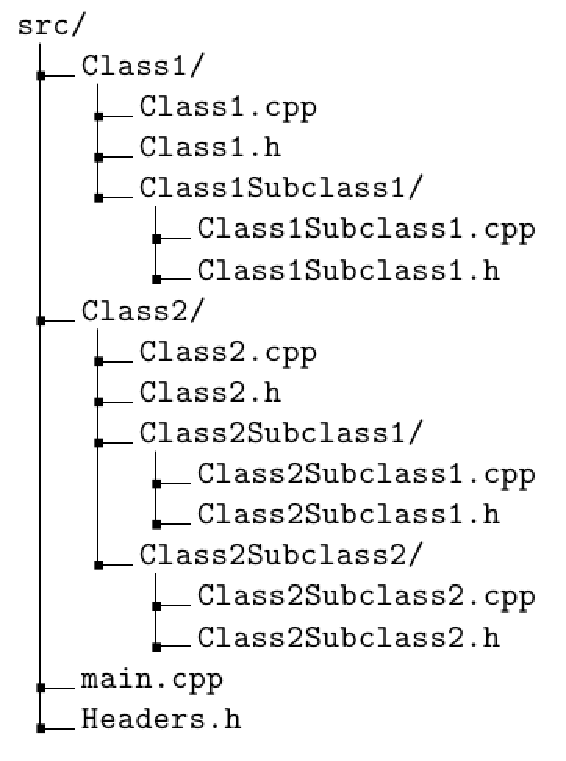
\includegraphics[scale=0.6]{../Graphics/SRCfolderStruct.pdf} 
 \end{center}
 \caption{An illustration of a standard way to organize source code. The file endings represent C++ code.}
\end{figure}


\subsection{Consistent Code Styles}

KEEP TO ONE STANDARD!

\subsection{Version Control}

USE E.G. GIT!
\chapter{Quantum Monte-Carlo}
\label{ch:QMC}

Quantum Monte-Carlo (QMC) is a method for solving Schrödinger's equation using statistical \textit{Markov Chain} (random walk) simulations. The statistical nature of Quantum Mechanics makes Monte-Carlo methods the perfect tool not only for accurately estimating observables, but also for extracting interesting quantities such as densities, i.e.~probability distributions. 

There are multiple strategies which can be used in order to deduce the virtual\footnote{As will be shown, the time parameter in QMC does not correspond to physical time, but rather an imaginary axis at a fixed point in time. Whether nature operates on a complex time plane or not is not testable in a laboratory, and the origin of the probabilistic nature of Quantum Mechanics will thus remain a philosophical problem.} dynamics of QMC, some of which are more mathematically complex than others. In this chapter the focus will be on modelling the Schrödinger equation as a diffusion problem in complex (Wick rotated) time. Other more condensed mathematical approaches does not need the Schrödinger equation at all, however, for the purpose of completeness, this approach will be mentioned only briefly in Section \ref{sec:ConnectAnisIs}.

In this chapter, \textit{Dirac Notation} will be used. See Appendix \ref{app:Dirac} for an introduction. The equations will be in atomic units, i.e. $\hbar = m_e = e = 4\pi\epsilon_0 = 1$, where $m_e$ and $\epsilon_0$ are the electron mass and the vacuum permittivity respectively.

\section{Modelling Diffusion}

Like any phenomena involving a probability distribution, Quantum Mechanics can be modelled by a diffusion process. In Quantum Mechanics, the distribution is given by $|\Ph|^2$, the wave function squared. The diffusing elements of interest are the particles in the system at hand. 

The basic idea is to introduce an ensemble of \textit{random walkers}, in which each walker is represented by a position in space at a given time. Once the walkers reach equilibrium, averaging values over the paths of the ensemble will yield average values corresponding to the probability distribution governing the movement of individual walkers. In other words: Counting every walker's contribution within a small volume $\mathrm{d}\mathbf{r}$ will correspond to $|\Ph|^2\mathrm{d}\mathbf{r}$ in the limit of infinite walkers.

Such random movement of walkers are referred to as a \textit{Brownian motion}, named after the British botanist R. Brown, originating from his experiments on plant pollen dispersed in water. Markov chains are a subtype of Brownian motion, where a walkers next move is independent of previous moves. This is the stochastic process in which QMC is described.

The purpose of this section is to motivate the use of diffusion theory in Quantum Mechanics, and to derive the sampling rules needed in order to model Quantum Mechanical distributions by diffusion of random walkers correctly. 

\subsection{Stating the Schrödinger Equation as a Diffusion Problem}
\label{sec:statingDiff}

Consider the time-dependent Schrödinger equation for an arbitrary wave function $\Ph$ using an arbitrary energy shift $E'$

\begin{equation}
 -\frac{\partial \Ph}{i\partial t} = (\OP{H} - E')\Ph.
\end{equation}

Given that the Hamiltonian is time-independent, the formal solution is found by separation of variables in $\Ph$ \cite{griffiths}

\begin{align}
 \OP{H}\Phn &= E\Phn, \label{eq:schrodTimeIndie}\\
 \Ph &= \exp\left(-i(\OP{H} - E')(t-t_0)\right)\Phn. \label{eq:schrodGeneralSolution}
\end{align}

From Eq.~(\ref{eq:schrodGeneralSolution}) it is apparent that the time evolution operator is on the form

\begin{equation}
 \OP{U}(t, t_0) = \exp\left(-i(\OP{H} - E')(t-t_0)\right). \label{eq:TimeEvolOp}
\end{equation}


The time-independent equation is solved for the ground state energy through methods such as \textit{Full Configuration Interaction} \cite{Shavitt} or similar methods based on diagonalizing the Hamiltonian. The time-dependent equation is used by methods such as \textit{Time-Dependent Multi-Configuration Hartree-Fock} \cite{Sigve} in order to obtain the time-development of quantum states. However, neither of the equations originate from, or resemble, diffusion equations. 

The original Schrödinger equation, however, does resemble a diffusion equation in complex time\footnote{The physical time diffusion equation evolves the squared wave function, and can be deduced from the quantum continuity equation combined with Fick's laws of diffusion \cite{QMCDIFF}.}. It can not be treated as a true diffusion equation, since the time evolved quantity, the wave function, is not a probability distribution unless it is squared. However, the equation involves a time derivative and a Laplacian, strongly indicating some sort of connection to a diffusion process.

Substituting complex time with a parameter $\tau$ and choosing the energy shift $E'$ equal to the true ground state energy of $\OP{H}$, $E_0$, the time evolution operator in Eq.~(\ref{eq:TimeEvolOp}) becomes the \textit{projection operation} $\OP{P}(\tau)$, whose choice of name will soon be apparent. In other words:

\begin{align}
t &\to it \equiv \tau,\notag\\
\OP{U}(t, 0) &\to \exp\left(-(\OP{H} - E_0)\tau\right) \equiv \OP{P}(\tau).\notag
\end{align}

Consider an arbitrary wave function $\PT$. Applying the new operator yields a new wave function $\Ptau$ in the following manner

\begin{align}
 \Ptau &= \bra{\mathbf{r}}\OP{P}(\tau)\ket{\Psi_T} \label{eq:projOPonTrial}\\
       &= \bra{\mathbf{r}}\exp\left(-(\OP{H} - E_0)\tau\right)\ket{\Psi_T}. \notag
\end{align}

Expanding the arbitrary state in the eigenfunction of $\OP{H}$, $\ket{\Psi_i}$, yields

\begin{align}
 \Ptau &= \sum_iC_i\bra{r}\exp\left(-(\OP{H} - E_0)\tau\right)\ket{\Psi_i}\notag \\
       &= \sum_iC_i\Psi_i(\mathbf{r})\exp\left(-(E_i - E_0)\tau\right) \notag \\
       &= C_0\Psi_0(x) + \sum_{i=1}^{\infty} C_i\Psi_k(x)e^{-\delta E_i\tau}, \label{eq:schrodGeneralSolution2}
\end{align}

where $C_i = \braket{\Psi_i}{\Psi_T}$ and $\delta E_i = E_i - E_0 \ge 0$. In the limit where $\tau$ goes to infinity, the ground state is the sole survivor of the expression, hence the name projection operator. In other words:

\begin{align}
 \lim_{\tau\to\infty}\Ptau &=  \lim_{\tau\to\infty}\bra{\mathbf{r}}\OP{P}(\tau)\ket{\Psi_T}\notag \\
                           &= C_0\Psi_0(x). \label{eq:ExactProjection}
\end{align}

The projection operator transforms an arbitrary wave function $\PT$, from here on referred to as the \textit{trial wave function}, into the true ground state, given that the overlap $C_0$ is non-zero.

In order to model the projection with Markov chains, the process needs to be split into subprocesses which in turn can be described as transitions in the Markov chain. Introducing a time-step $\delta\tau$, the projection operator can be rewritten as

\begin{equation}
 \OP{P}(\tau) = \prod_{k=1}^n \exp\left(-(\OP{H} - E_0)\delta\tau\right),
\end{equation}

where $n = \tau/\delta\tau$. An important property to notice is that

\begin{equation}
 \OP{P}(\tau + \delta\tau) = \exp\left(-(\OP{H} - E_0)\delta\tau\right)\OP{P}(\tau).
\end{equation}

Using this relation in combination with Eq.~(\ref{eq:projOPonTrial}), the effect of the projection operator during a single time-step is revealed:

\begin{align}
 \Phi(\mathbf{r}, \tau + \delta\tau) &= \bra{\mathbf{r}}\OP{P}(\tau + \delta\tau)\ket{\Psi_T} \notag \\
    &= \bra{\mathbf{r}} \exp\left(-(\OP{H} - E_0)\delta\tau\right)\OP{P}(\tau)\ket{\Psi_T} \notag \\
    &=  \bra{\mathbf{r}} \exp\left(-(\OP{H} - E_0)\delta\tau\right)\ket{\Phi(\tau)} \notag \\
    &= \int_{\mathbf{r}'}\bra{\mathbf{r}}\exp\left(-(\OP{H} - E_0)\delta\tau\right)\ket{\mathbf{r}'}\braket{\mathbf{r}'}{\Phi(\tau)}\mathrm{d}\mbf{r}' \notag \\
    &= \int_{\mathbf{r}'}\bra{\mathbf{r}}\exp\left(-(\OP{H} - E_0)\delta\tau\right)\ket{\mathbf{r}'}\Phi(\mbf{r}', \tau)\mathrm{d}\mbf{r}',
\end{align}

where a complete set of position states were introduced.

For practical purposes, $E_0$ needs to be substituted with an approximation $E_T$ to the ground state energy, commonly referred to as the \textit{trial energy}, in order to avoid self consistency. From Eq.~(\ref{eq:schrodGeneralSolution2}) it is apparent that the projection will still converge as long as $E_T < E_1$, that is, the trial energy is less than that of the first excitation. The resulting expression reads:

\begin{align}
 \Phi(\mathbf{r}, \tau + \delta\tau) &= \int_{\mathbf{r}'}\bra{\mathbf{r}}\exp\left(-(\OP{H} - E_T)\delta\tau\right)\ket{\mathbf{r}'}\Phi(\mbf{r}', \tau)\mathrm{d}\mbf{r}' \\
  &\equiv \int_{\mathbf{r}'}G(\mbf{r}, \mbf{r'}; \delta\tau)\Phi(\mbf{r}', \tau)\mathrm{d}\mbf{r}'.  \label{eq:QMC_GF_EQ}
\end{align}

The equations above are well suited for Markov Chain models, as an ensemble of walkers can be iterated by transitioning between configurations $\ket{\mbf{r}}$ and $\ket{\mbf{r}'}$ with probabilities given by the \textit{Green's function}, $G(\mbf{r}, \mbf{r'}; \delta\tau).$

The effect of the Green's function from Eq.~(\ref{eq:QMC_GF_EQ}) on individual walkers is not trivial. In order to relate the Green's function to well-known processes, the exponential is split into two parts, one containing only the kinetic energy operator $\OP{T} = -\frac{1}{2}\nabla^2$, and the second containing the potential energy operator $\OP{V}$ and the energy shift. This is known as the \textit{short time approximation}\cite{abInitioMC}

\begin{align}
  G(\mbf{r}, \mbf{r'}; \delta\tau) &= \bra{\mathbf{r}}\exp\left(-(\OP{H} - E_T)\delta\tau\right)\ket{\mathbf{r}'} \label{eq:firstTrialEnergyIntro} \\
  &= \bra{\mathbf{r}}e^{-\OP{T}\delta\tau}e^{-(\OP{V} - E_T)\delta\tau}\ket{\mathbf{r}'} + \frac{1}{2}[\OP{V}, \OP{T}]\delta\tau^2 + \mathcal{O}(\delta\tau^3).  \label{eq:shortTimeApprox}
\end{align}

The first exponential describes a transition of walkers governed by the Laplacian, which is a diffusion process. The second exponential is linear in position space and is thus a weighing function responsible for distributing the correct weights to the corresponding walkers. In other words:

\begin{eqnarray}
 G_\mathrm{Diff} &=& e^{\frac{1}{2}\nabla^2\delta\tau},\label{eq:GDiff} \\
 G_\mathrm{B} &=& e^{-(\OP{V} - E_T)\delta\tau} \label{eq:GB},
\end{eqnarray}

where $B$ denotes \textit{branching}. The reasons for this name together with the complete process of modelling weights by branching will be covered in detail in Section \ref{sec:branching}.

The flow of QMC is then to use these Green's functions to propagate the ensemble of walkers into the next time-step. The final distribution of walkers will correspond to that of the direct solution of the Schrödinger equation, given that the time-step is sufficiently small, and the number of cycles $n$ are sufficiently large. These constraints will be covered in more detail later. 

Incorporating only the effect of Eq.~(\ref{eq:GDiff}) results in a method called \textit{Variational Monte-Carlo} (VMC). Including the branching term as well results in \textit{Diffusion Monte-Carlo} (DMC). These methods will be discussed in Sections \ref{sec:VMC} and \ref{sec:DMC} respectively. In either of these methods, diffusion is a key process.

\section{Solving the Diffusion Problem}
\label{sec:solvingDiff}

The diffusion problem introduced in the previous section uses a symmetric kinetic energy operator implying an \textit{isotropic diffusion}, however, a more efficient kinetic energy operator can be introduced without violating the original equations, resulting in an \textit{anisotropic diffusion} governed by the \textit{Fokker-Planck equation}. These models will be the topic of this section. 

For details regarding the transition from isotropic to anisotropic diffusion, see Section \ref{sec:ConnectAnisIs}.

\subsection{Isotropic Diffusion}

Isotropic diffusion is a process in which diffusing particles sees all directions as an equally probable path. Eq.~(\ref{Eq:diffusionSimple}) is an example of this. The isotropic diffusion equation is  

\begin{equation}
 \label{Eq:diffusionSimple}
 \frac{\partial P(\mbf{r}, t)}{\partial t} = D\nabla^2 P(\mbf{r}, t) .
\end{equation}

This is the simplest form of a diffusion equation, that is, the case with a linear \textit{diffusion constant}, $D$, and no drift terms. 

From Eq.~(\ref{eq:GDiff}) it is clear that the value of the diffusion constant is $D=\frac{1}{2}$, originating from the term scaling the Laplacian in the Schrödinger Equation. An important point is that closed form expressions for the Green's function exists. This closed form expression in the isotropic case is a Gaussian distribution with variance $2D\delta t$ \cite{abInitioMC}

\cfbox{-6pt}{
\begin{equation}
\label{eq:GF_iso}
 G_{\mathrm{Diff}}^{\mathrm{ISO}}(i\,\rightarrow\,j) \propto e^{-|\mbf{r}_i-\mbf{r}_j|^2/4D\delta\tau} .
\end{equation}
}

These equations describe the diffusion process theoretically, however, in order to achieve specific sampling rules for the walkers, a connection between the time-dependence of the distribution and the time-dependence of an individual walker's components in configuration space is needed. This connection is given in terms of a stochastic differential equation called \textit{The Langevin Equation}.

\subsubsection{The Langevin Equation for isotropic diffusion}

The Langevin Equation is a stochastic differential equation used in physics to relate the time dependence of a distribution to the time-dependence of the degrees of freedom in a system. For isotropic diffusion, solving the Langevin equation using a Forward Euler approximation for the time derivative results in the following relation:

\begin{eqnarray}
\label{eq:langevinSolSimple}
 x_{i+1} = x_i + \xi, \qquad\qquad \mathrm{Var}(\xi) &=& 2D\delta t, \\
			     \langle\xi\rangle &=& x_i, \nonumber 
\end{eqnarray}

where $\xi$ is a normal distributed number whose variance matches that of the Green's function in Eq.~(\ref{eq:GF_iso}). This relation is in agreement with the isotropy of Eq.~(\ref{Eq:diffusionSimple}) in the sense that the displacement is symmetric around the current position.


\subsection{Anisotropic Diffusion and the Fokker-Planck equation}
\label{sec:anisFokker}

Anisotropic diffusion, in contrast to isotropic diffusion, does not see all directions as equally probable. An example of this is diffusion according to the \textit{Fokker-Planck Equation}, that is, diffusion with a drift term, $\mbf{F}(\mbf{r}, t)$, responsible for pushing the walkers in the direction of configurations with higher probabilities, and thus closer to an equilibrium state. The Fokker-Planck equation reads:

\begin{equation}
 \label{Eq:fokkerPlanck}
 \frac{\partial P(\mbf{r}, t)}{\partial t} = D\nabla\cdot\Big[\Big(\nabla - \mbf{F}(\mbf{r}, t)\Big) P(\mbf{r}, t)\Big] .
\end{equation}

As will be derived in detail in Section \ref{sec:ConnectAnisIs}, using the Fokker-Planck equation does not violate the original Schrödinger equation, but changes the representation of the ensemble of walkers to a mixed density. This means that QMC can be run with Fokker-Planck diffusion, leading to a more optimized way of sampling due to the drift term. 

As mentioned introductory, the goal of the Markov process is convergence to a stationary state. Using this criteria, the expression for the drift term can be found. A stationary state is obtained when the left hand side of Eq.~(\ref{Eq:fokkerPlanck}) is zero. This yields:

\begin{equation*}
 \nabla^2 P(\mbf{r}, t) = P(\mbf{r}, t)\nabla\cdot\mbf{ F}(\mbf{ r}, t) + \mbf{ F}(\mbf{ r}, t) \cdot \nabla P(\mbf{ r}, t).
\end{equation*}

In order to get cancellation in the remaining terms, the Laplacian term on the right-hand side must cancel out the terms on the left. This implies that the drift term needs to be on the form $\mbf{F}(\mbf{ r}, t) = g(\mbf{ r}, t)\nabla P(\mbf{ r}, t)$. Inserting this yields

\begin{equation*}
  \nabla^2 P(\mbf{ r}, t) = P(\mbf{ r}, t)\frac{\partial g(\mbf{ r}, t)}{\partial P(\mbf{ r}, t)}\Big|\nabla P(\mbf{ r}, t)\Big|^2
  + P(\mbf{ r}, t)g(\mbf{ r}, t)\nabla^2 P(\mbf{ r}, t) + g(\mbf{ r}, t) \Big|\nabla P(\mbf{ r}, t)\Big|^2.
\end{equation*}

The factors in front of the Laplacian suggests using $g(\mbf{ r}, t) = 1/P(\mbf{ r}, t)$. A quick check reveals that this also cancels the gradient terms. The resulting expression for the drift term becomes

\cfbox{3mm -5pt}{
\begin{eqnarray}
 \mbf{ F}(\mbf{ r}, t) &=& \frac{1}{P(\mbf{ r}, t)}\nabla P(\mbf{ r}, t) \nonumber \\
                   &=& \frac{2}{|\psi(\mbf{ r}, t)|}\nabla |\psi(\mbf{ r}, t)|. \\
                   \nonumber
\end{eqnarray}
}


In QMC, the drift term is commonly referred to as the \textit{quantum force}. This is due to the fact that it is responsible for pushing the walkers into regions of higher probabilities, analogous to a force in Newtonian mechanics.

Another strength of the Fokker-Planck equation is that even though the equation itself is more complicated, its Green's function still has a closed form solution. This means that it can be evaluated efficiently. If this was not the case, the practical value would be reduced dramatically. The reason for this will become clear in Section \ref{sec:MetroMain}. The closed form solution reads \cite{abInitioMC}

\cfbox{5mm-7pt}{
\begin{equation}
\label{eq:GF_FP}
 G_\mathrm{Diff}^\mathrm{FP}(i\,\rightarrow j) \propto e^{-(x_i-x_j - D\delta\tau F(x_i))^2/4D\delta\tau}.
\end{equation}
}

As expected, the Green's function is no longer symmetric.

\subsubsection{The Langevin Equation for the Fokker-Planck equation}

The Langevin equation in the case of a Fokker-Planck Equation has the following form

\begin{equation}
 \frac{\partial x_i}{\partial t} = D F(\mbf{r})_i + \eta,
\end{equation}

where $\eta$ is a so-called \textit{noise term} from stochastic processes. Solving this equation using the same method as for the isotropic case yields the following sampling rules

\begin{equation}
 \label{eq:langevinSolFP}
 x_{i+1} = x_i + \xi + DF(\mbf{r})_i\delta t,
\end{equation}

where $\xi$ is the same as for the isotropic case. Observe that when the drift term goes to zero, the Fokker-Planck - and isotropic solutions are equal, just as required. For more details regarding the Fokker-Planck Equation and Langevin equations, see Refs. \cite{Gardiner:2004bk, risken1989fpe, langevin}.


\subsection{Connecting Anisotropic - and Isotropic Diffusion Models}
\label{sec:ConnectAnisIs}

To this point, it might seem far-fetched that switching the diffusion model to a Fokker-Planck diffusion does not violate the original equation, i.e. the complex time Schrödinger equation (the projection operator). Introducing the distribution function $f(\mbf{r}, t) = \Phi(\mbf{r}, t)\Psi_T(\mbf{r})$, restating the imaginary time Schrödinger equation in terms of $f(\mbf{r}, t)$ yields

\begin{eqnarray}
-\frac{\partial}{\partial t}f(\mbf{r}, t)\,\, = \,\,\Psi_T(\mbf{r})\Big[-\frac{\partial}{\partial t}\Phi(\mbf{r}, t)\Big] &=& \Psi_T(\mbf{r})\left(\OP{H} - E_T\right)\Phi(\mbf{r}, t) \nonumber\\
         &=& \Psi_T(\mbf{r})\left(\OP{H} - E_T\right)\Psi_T(\mbf{r})^{-1}f(\mbf{r}, t) \label{eq:impSamplRaw}\\
         &=& -\frac{1}{2}\Psi_T(\mbf{r})\nabla^2 \left(\Psi_T(\mbf{r})^{-1}f(\mbf{r}, t)\right) + \OP{V}f(\mbf{r}, t) - E_Tf(\mbf{r},t).\nonumber
\end{eqnarray}

Expanding the Laplacian term further reveals

\begin{eqnarray}
K(\mbf{r}, t) &\equiv& -\frac{1}{2}\Psi_T(\mbf{r})\nabla^2 \left(\Psi_T(\mbf{r})^{-1}f(\mbf{r}, t)\right) \nonumber\\
 &=& -\frac{1}{2}\Psi_T(\mbf{r})\nabla\cdot (\nabla\left[\Psi_T(\mbf{r})^{-1}f(\mbf{r}, t)\right]), \\
\nabla\left[\Psi_T(\mbf{r})^{-1}f(\mbf{r}, t)\right] &=& -\Psi_T(\mbf{r})^{-2}\nabla \Psi_T(\mbf{r}) f(\mbf{r}, t) + \Psi_T(\mbf{r})^{-1}\nabla f(\mbf{r}, t).
\end{eqnarray}

Combining these equations and applying the product rule numerous times yield

\begin{eqnarray*}
K(\mbf{r}, t) &=& -\frac{1}{2}\Psi_T(\mbf{r})\Big[\big(2\Psi_T(\mbf{r})^{-3}\left|\nabla\Psi_T(\mbf{r})\right|^2f(\mbf{r}, t) \\
        & & - \Psi_T(\mbf{r})^{-2}\nabla^2\Psi_T(\mbf{r})f(\mbf{r}, t) \\
        & & - \Psi_T(\mbf{r})^{-2}\nabla\Psi_T(\mbf{r})\cdot\nabla f(\mbf{r}, t)\big) \\
        & & + \Psi_T(\mbf{r})^{-1}\nabla^2 f(\mbf{r}, t) \\
        & & - \Psi_T(\mbf{r})^{-2}\nabla\Psi_T(\mbf{r})\cdot\nabla f(\mbf{r}, t)\Big] \\
        &=& - \left|\Psi_T(\mbf{r})^{-1}\nabla\Psi_T(\mbf{r})\right|^2f(\mbf{r}, t) \\
        & & + \frac{1}{2}\Psi_T(\mbf{r})^{-1}\nabla^2\Psi_T(\mbf{r})f(\mbf{r}, t) \\
        & & + \Psi_T(\mbf{r})^{-1}\nabla\Psi_T(\mbf{r})\cdot\nabla f(\mbf{r}, t) \\
        & & - \frac{1}{2}\nabla^2 f(\mbf{r}, t). \\
\end{eqnarray*}

Introducing the following identity helps clean up the messy calculations:

\begin{eqnarray*}
%  \nabla\cdot\left(\Psi_T(\mbf{r})^{-1}\nabla\Psi_T(\mbf{r})\right) &=& -\Psi_T(\mbf{r})^{-2}\left|\nabla\Psi_T(\mbf{r})\right|^2 + \Psi_T(\mbf{r})^{-1}\nabla^2\Psi_T(\mbf{r}) \\
 -\left|\Psi_T(\mbf{r})^{-1}\nabla\Psi_T(\mbf{r})\right|^2 &=& \nabla\cdot\left(\Psi_T(\mbf{r})^{-1}\nabla\Psi_T(\mbf{r})\right) - \Psi_T(\mbf{r})^{-1}\nabla^2\Psi_T(\mbf{r}),
\end{eqnarray*}

which inserted into the expression for $K(\mbf{r}, t)$ reveals

\begin{eqnarray*}
K(\mbf{r}, t) &=&  \nabla\cdot\left(\Psi_T(\mbf{r})^{-1}\nabla\Psi_T(\mbf{r})\right)f(\mbf{r}, t) \\
        & & + \left(\frac{1}{2} - 1\right)\Psi_T(\mbf{r})^{-1}\nabla^2\Psi_T(\mbf{r})f(\mbf{r}, t) \\
        & & + \Psi_T(\mbf{r})^{-1}\nabla\Psi_T(\mbf{r})\cdot\nabla f(\mbf{r}, t) \\
        & & - \frac{1}{2}\nabla^2 f(\mbf{r}, t). \\
\end{eqnarray*}

Inserting the expression for the quantum force $\mbf{F}(\mbf{r}) = 2\Psi_T(\mbf{r})^{-1}\nabla\Psi_T(\mbf{r})$ and the local kinetic energy $K_L(\mbf{r}) = -\frac{1}{2}\Psi_T(\mbf{r})^{-1}\nabla^2\Psi_T(\mbf{r})$ simplifies the expression dramatically

\begin{eqnarray*}
 K(\mbf{r}, t) &=& - \frac{1}{2}\nabla^2 f(\mbf{r}, t) + \frac{1}{2}\underbrace{\left[\mbf{F}(\mbf{r})\cdot \nabla f(\mbf{r}, t) + f(\mbf{r}, t)\nabla\cdot \mbf{F}(\mbf{r})\right]}_{\nabla\cdot\left[\mbf{F} f(\mbf{r}, t)\right]} + K_L(\mbf{r})f(\mbf{r}, t)\\
         &=& \frac{1}{2}\nabla\cdot \left[\left(\nabla - \mbf{F}(\mbf{r})\right)f(\mbf{r}, t)\right] + K_L(\mbf{r})f(\mbf{r}, t).
\end{eqnarray*}

Inserting everything back into Eq.~(\ref{eq:impSamplRaw}) yields

\begin{eqnarray}
 -\frac{\partial}{\partial t}f(\mbf{r}, t) &=& -\frac{1}{2}\nabla\cdot \left[\left(\nabla - \mbf{F}(\mbf{r})\right)f(\mbf{r}, t)\right] + K_L(\mbf{r})f(\mbf{r}, t) + \OP{V}f(\mbf{r}, t) - E_Tf(\mbf{r},t) \nonumber\\
  \frac{\partial}{\partial t}f(\mbf{r}, t)  &=& \frac{1}{2}\nabla\cdot \left[\left(\nabla - \mbf{F}(\mbf{r})\right)f(\mbf{r}, t)\right] - \left(E_L(\mbf{r}) - E_T\right)f(\mbf{r}, t), 
\end{eqnarray}

which is the Fokker-Planck diffusion equation from Eq.~(\ref{Eq:fokkerPlanck}) with a constant shift representing the branching Green's function in the case Fokker-Planck diffusion.

Just as in traditional importance sampled Monte-Carlo integrals, optimized sampling is obtained in QMC by switching distributions into one which exploits known information about the problem at hand. In the case of standard Monte-Carlo integration, the sampling distribution is substituted with one which are similar to the original integrand, resulting in a smoother sampled function, where as in QMC, a distribution is constructed with the sole purpose of imitating the exact ground state in order to suggest moves more efficiently. It is therefore reasonable to call the use of Fokker-Planck diffusion \textit{importance sampled} QMC.

The energy estimated using the new distribution $f(\mbf{r}, t)$ will still equal the exact energy in the limit of convergence. This is demonstrated in the following equations:

\begin{align*}
 E_\mathrm{QMC} &= \frac{1}{N}\int f(\mbf{r}, \tau) \frac{1}{\Psi_T(\mbf{r})} \OP{H} \Psi_T(\mbf{r}) \mathrm{d}\mbf{r} \\
                &= \frac{1}{N}\int \Phi(\mbf{r}, \tau) \OP{H} \Psi_T(\mbf{r}) \mathrm{d}\mbf{r} \\
                &= \frac{1}{N}\bra{\Phi(\tau)}\OP{H}\ket{\Psi_T}, \\
\end{align*}
where 
\begin{align*}
               N&= \int f(\mbf{r}, \tau) \mathrm{d}\mbf{r} \\
                &= \int \Phi(\mbf{r}, \tau)\Psi_T(\mbf{r})\mathrm{d}\mbf{r} \\
                &= \braket{\Phi(\tau)}{\Psi_T},\\
 \end{align*}
which results in the following expression for the energy:
\begin{align*}               
 E_\mathrm{QMC} &= \frac{\bra{\Phi(\tau)}\OP{H}\ket{\Psi_T}}{\braket{\Phi(\tau)}{\Psi_T}}.\\
\end{align*}

Assuming that the walkers have converged to the exact ground state, i.e.~$\ket{\Phi(\tau)}=\ket{\Phi_0}$, letting the Hamiltonian work to the left yields

\begin{align*}
 E_\mathrm{QMC} &= E_0\frac{\braket{\Phi_0}{\Psi_T}}{\braket{\Phi_0}{\Psi_T}} \\
                &= E_0.
\end{align*}

Estimating the energy in QMC will be discussed in detail in Sections \ref{sec:calcExpVals} and \ref{sec:DMC}. 

\section{Diffusive Equilibrium Constraints}

Upon convergence of a Markov process, the ensemble of walkers will on average span the system's most likely state. This is exactly the behavior of a system of diffusing particles described by statistical mechanics: It will \textit{thermalize}, that is, reach equilibrium. 

Once thermalization is reached, expectation values may be sampled. However, simply spawning a Markov process and waiting for thermalization is an inefficient and unpractical scenario. This may take forever, or it may not; either way it is not optimal. Introducing rules of acceptance and rejection on top of the suggested transitions given by the Langevin equation in Eq.~(\ref{eq:langevinSolSimple} or Eq.~(\ref{eq:langevinSolFP}) will result in an optimized sampling. Special care must be taken not to violate necessary properties of the Markov process. If any of the conditions discussed in this section break, there is no guarantee that the system will thermalize properly.

\subsection{Detailed Balance} 

For Markov processes, detailed balance is achieved by demanding a \textit{reversible} Markov process. This boils down to a statistical requirement stating that 

\begin{equation}
 \label{eq:DetailedBalance}
 P_iW(i\,\rightarrow\,j) = P_jW(j\,\rightarrow\,i),
\end{equation}

where $P_i$ is the probability density in configuration $i$, and $W(i\,\rightarrow\,j)$ is the transition probability between states $i$ and $j$. 

\subsection{Ergodicity}

Another requirement is that the sampling must be \textit{ergodic} \cite{robertcasella}, that is, the random walkers need to be able to reach any configuration in the space spanned by the distribution function. It is tempting to define a brute force acceptance rule where only steps resulting in a higher overall probability is accepted, however, this limits the path of the walker, and will thus break the requirement of ergodicity.

\section{The Metropolis Algorithm}
\label{sec:MetroMain}

The Metropolis Algorithm is a simple set of acceptance/rejection rules used in order to make the thermalization more efficient. For a given probability distribution function $P$, the Metropolis algorithm will force sampled points to follow this distribution. 

Starting from the criteria of detailed balance given in Eq.~(\ref{eq:DetailedBalance}, and further introducing a model for the transition probability $W(i\,\rightarrow\,j)$ as consisting of two parts: The probability of selecting configuration $j$ given configuration $i$, $g(i\,\rightarrow\,j)$, times a probability of accepting the selected move, $A(i\,\rightarrow\,j)$, yields

\begin{eqnarray}
 \label{eq:metro1}
 P_iW(i\,\rightarrow\,j) &=& P_jW(j\,\rightarrow\,i), \nonumber \\
 P_ig(i\,\rightarrow\,j)A(i\,\rightarrow\,j) &=& P_jg(j\,\rightarrow\,i)A(j\,\rightarrow\,i).
\end{eqnarray}

Inserting the probability distribution as the wave function squared and the selection probability as the Green's function, the expression becomes

\begin{eqnarray}
  \label{eq:metro2}
  |\psi_i|^2G(i\,\rightarrow\,j)A(i\,\rightarrow\,j) &=& |\psi_j|^2G(j\,\rightarrow\,i)A(j\,\rightarrow\,i), \nonumber \\
  \frac{A(j\,\rightarrow\,i)}{A(i\,\rightarrow\,j)} &=& \frac{G(i\,\rightarrow j)}{G(j\,\rightarrow i)}\frac{|\psi_i|^2}{|\psi_j|^2} \equiv R_G(j\,\rightarrow\,i)R_\psi(j\,\rightarrow\,i)^2,
\end{eqnarray}

where the defined ratios correspond to the Green's function - and wave function ratio respectively. 

Assume now that configuration $i$ has a higher overall probability than configuration $j$. The essence of the Metropolis algorithm is that the step is automatically accepted, that is, $A(i\,\rightarrow\,j) = 1$. In other words, a more efficient thermalization is obtained by accepting all these moves. What saves Metropolis from breaking the criteria of ergodicity, is the fact that suggested moves to lower probability states are not automatically rejected. This is demonstrated by solving Eq.~(\ref{eq:metro2}) for the case where $A(i\,\rightarrow\,j) = 1$, that is, the case where $P_i < P_j$. This yields

\begin{equation*}
 A(j\,\rightarrow\,i) = R_G(j\,\rightarrow\,i)R_\psi(j\,\rightarrow\,i)^2.
\end{equation*}


Combining both scenarios into one expression yield the following acceptance/rejection rules:

\cfbox{10mm - 14pt}{
\begin{equation}
\label{eq:MetroGeneralGreen}
 A(i\,\rightarrow\,j) = \left\{\begin{array}{ccc}
R_G(i\,\rightarrow\,j)R_\psi(i\,\rightarrow\,j)^2 & & R_G(i\,\rightarrow\,j)R_\psi(i\,\rightarrow\,j)^2 < 1\\
1  & & \mathrm{else}  \end{array}\right. .
\end{equation}
}

This equation can be simplified to

\begin{equation}
  A(i\,\rightarrow\,j) = \min\{R_G(i\,\rightarrow\,j)R_\psi(i\,\rightarrow\,j)^2, \,1\}.
\end{equation}


In the isotropic diffusion case, the Green's function ratio cancels due to symmetry, i.e.~$R_G(i\,\rightarrow\,j) = 1$, resulting in the standard Metropolis algorithm:

\begin{equation}
\label{eq:Metropolis_standard}
 A(i\,\rightarrow\,j) = \min\{R_\psi(i\,\rightarrow\,j)^2, \,1\}.
\end{equation}

On the other hand, for Fokker-Planck diffusion, there will be no cancellation of the Green's functions. Inserting Eq.~(\ref{eq:GF_FP}) into Eq.~(\ref{eq:MetroGeneralGreen}) results in the \textit{Metropolis Hastings algorithm} \cite{robertcasella}. The ratio of the Green's functions can be evaluated efficiently by simply subtracting the exponents of the exponentials. This is best demonstrated by calculating the logarithm

\begin{eqnarray}
 \log{R_G^\mathrm{FP}(i\,\rightarrow\,j)} &=& \log \left(G_\mathrm{Diff}^\mathrm{FP}(j\,\rightarrow i)/G_\mathrm{Diff}^\mathrm{FP}(i\,\rightarrow j)\right) \nonumber \\
                                    &=& \frac{1}{2}\big(F(x_j) + F(x_i)\big)\big(\frac{1}{2}D\delta t(F(x_j) - F(x_i)) + x_i - x_i\big), \\
                                    \nonumber\\
 A(i\,\rightarrow\,j) &=& \min\{\exp \left(\log R_G^\mathrm{FP}(i\,\rightarrow\,j)\right)R_\psi(i\,\rightarrow\,j)^2, \,1\}. \label{eq:MetropolisHastings}
\end{eqnarray}

Derived from detailed balance, the Metroplis Algorithm is an essential part of any Markov Chain Monte-Carlo algorithm. Besides QMC, methods for solving problems such as the \textit{Ising Model} greatly benefit from these rules \cite{morten}.

In practice, without the Metropolis sampling, the ensemble of walkers will not span that of the trial wave function. This is due to the fact that the time-step used in the simulations is finite, and the trial positions of the walkers are random. A chart flow describing the implementation of the Metropolis algorithm and the diffusion process is given in Figure \ref{fig:diffFlowChart}.

\begin{figure}
 \begin{center}
  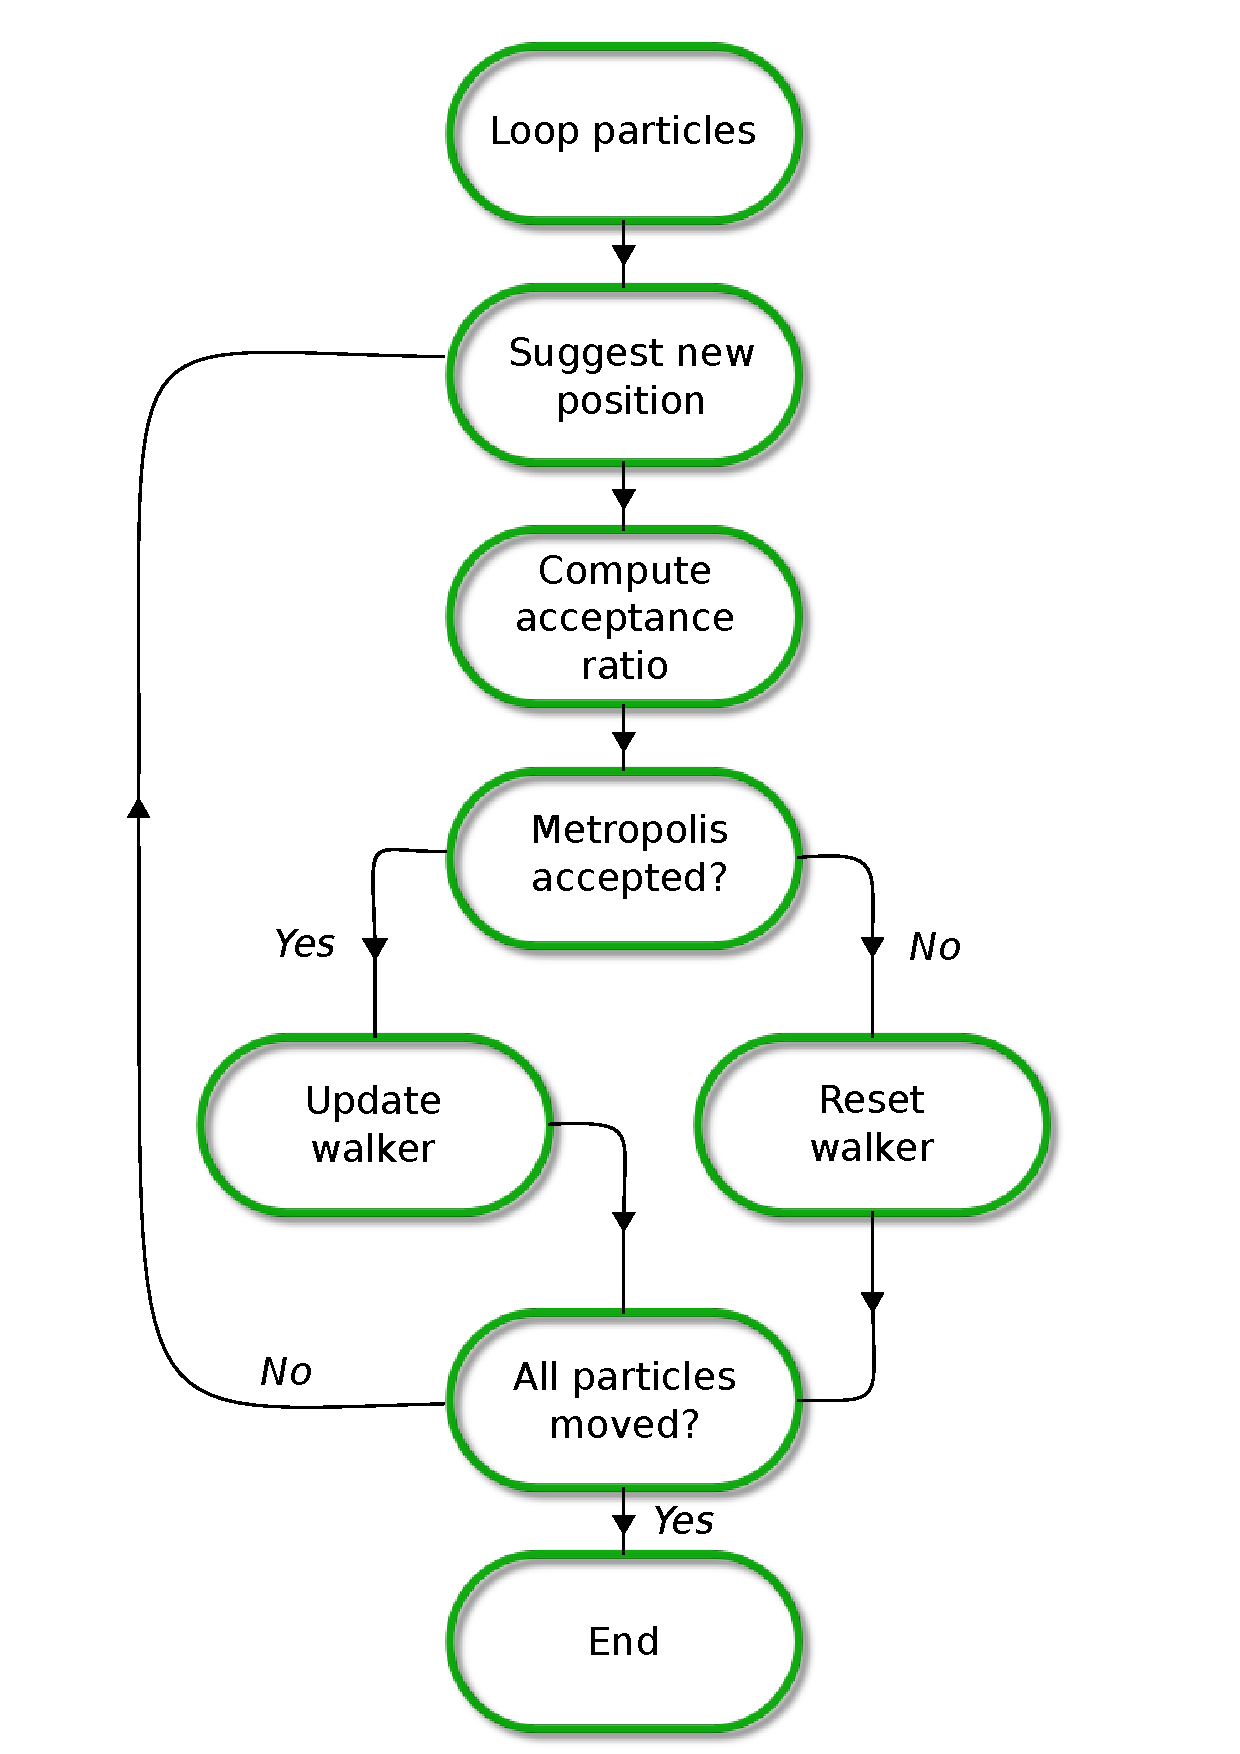
\includegraphics[scale=0.65]{../Graphics/DiffusionUML.pdf}
  \caption{Flow chart describing the process of iterating a walker through a single time-step, that is, simulation the application of the Green's function from Eq.~(\ref{eq:GDiff}) using the Metropolis algorithm. New positions are suggested according to the chosen diffusion model.}
  \label{fig:diffFlowChart}
 \end{center}
\end{figure}
\clearpage




\section{The Process of Branching}
\label{sec:branching}

In the previous section it became clear that the Metropolis test will guide the walkers to span a distribution representing the trial wave function. This implies that without further action, no changes to the distribution can be made, and the point of modelling the projection operator from Eq.~(\ref{eq:projOPonTrial}) is rendered useless. The important fact to include is that the branching Green's function from Eq.~(\ref{eq:branchFP}) and Eq.~(\ref{eq:branchISO}) distribute weights to the walkers, effectively altering the spanned distribution. 

The process of branching in QMC is simulated by the creation and destruction of walkers with probability equal to that of the branching Green's function \cite{abInitioMC}. The explicit shapes in case of isotropic - (ISO) and anisotropic diffusion (FP) are

\begin{eqnarray}
 G_B^\mathrm{ISO}(i\,\rightarrow j) &=& e^{-\left(\frac{1}{2}\left[V(x_i) + V(x_j)\right] - E_T\right)\delta\tau}\label{eq:branchISO}, \\
 G_B^\mathrm{FP}(i\,\rightarrow j) &=& e^{-\left(\frac{1}{2}\left[E_L(x_i) + E_L(x_j)\right] - E_T\right)\delta\tau}, \label{eq:branchFP}
\end{eqnarray}

where $E_L(x_i)$ is the energy evaluated in configuration $x_i$ (see Section \ref{sec:calcExpVals} for details). The three different scenarios which arise is

\begin{itemize}
 \item $G_B = 1$ : No branching.
 \item $G_B = 0$ : The current walker is to be removed from the current ensemble.
 \item $G_B > 1$ : On average $G_B - 1$ replicas of the current walker are made.
\end{itemize}

Defining the following quantity allows for an efficient simulation of this behavior

\cfbox{1.1cm-10pt}{
\begin{equation}
 \overline{G}_B = \mathrm{floor}\left(G_B + a\right),\label{eq:gbMean}
\end{equation}
}


where $a$ is a uniformly distributed number on $[0,1)$. The probability that $\overline{G}_B = G_B + 1$ is then equal to $G_B - \mathrm{floor}(G_B)$. As an example, assume $G_B = 3.3$. The value of $\overline{G}_B$ is then either three or four, depending on whether $a < 0.7$ or not. The probability that $a<0.7$ is obviously $70\%$, implying that there is a $30\%$ chance that $\overline{G}_B$ is equal to four, and $70\%$ chance that is is equal to three. 

There are some programming challenges due to the fact that the number of walkers is not conserved, such as cleaning up inactive walkers and stabilizing the population across different computational nodes. For details regarding this, see the code documentation at Ref. \cite{libBorealisCode}. Isotropic diffusion is in practice never used with branching due to the singularities in the Coulomb interaction (see Eq.~(\ref{eq:branchISO})). This singularity may cause large fluctuations in the walker population, which is far from an optimal behavior.

The process of branching is demonstrated in Figure \ref{fig:branching}.

\begin{figure}
 \begin{center}
  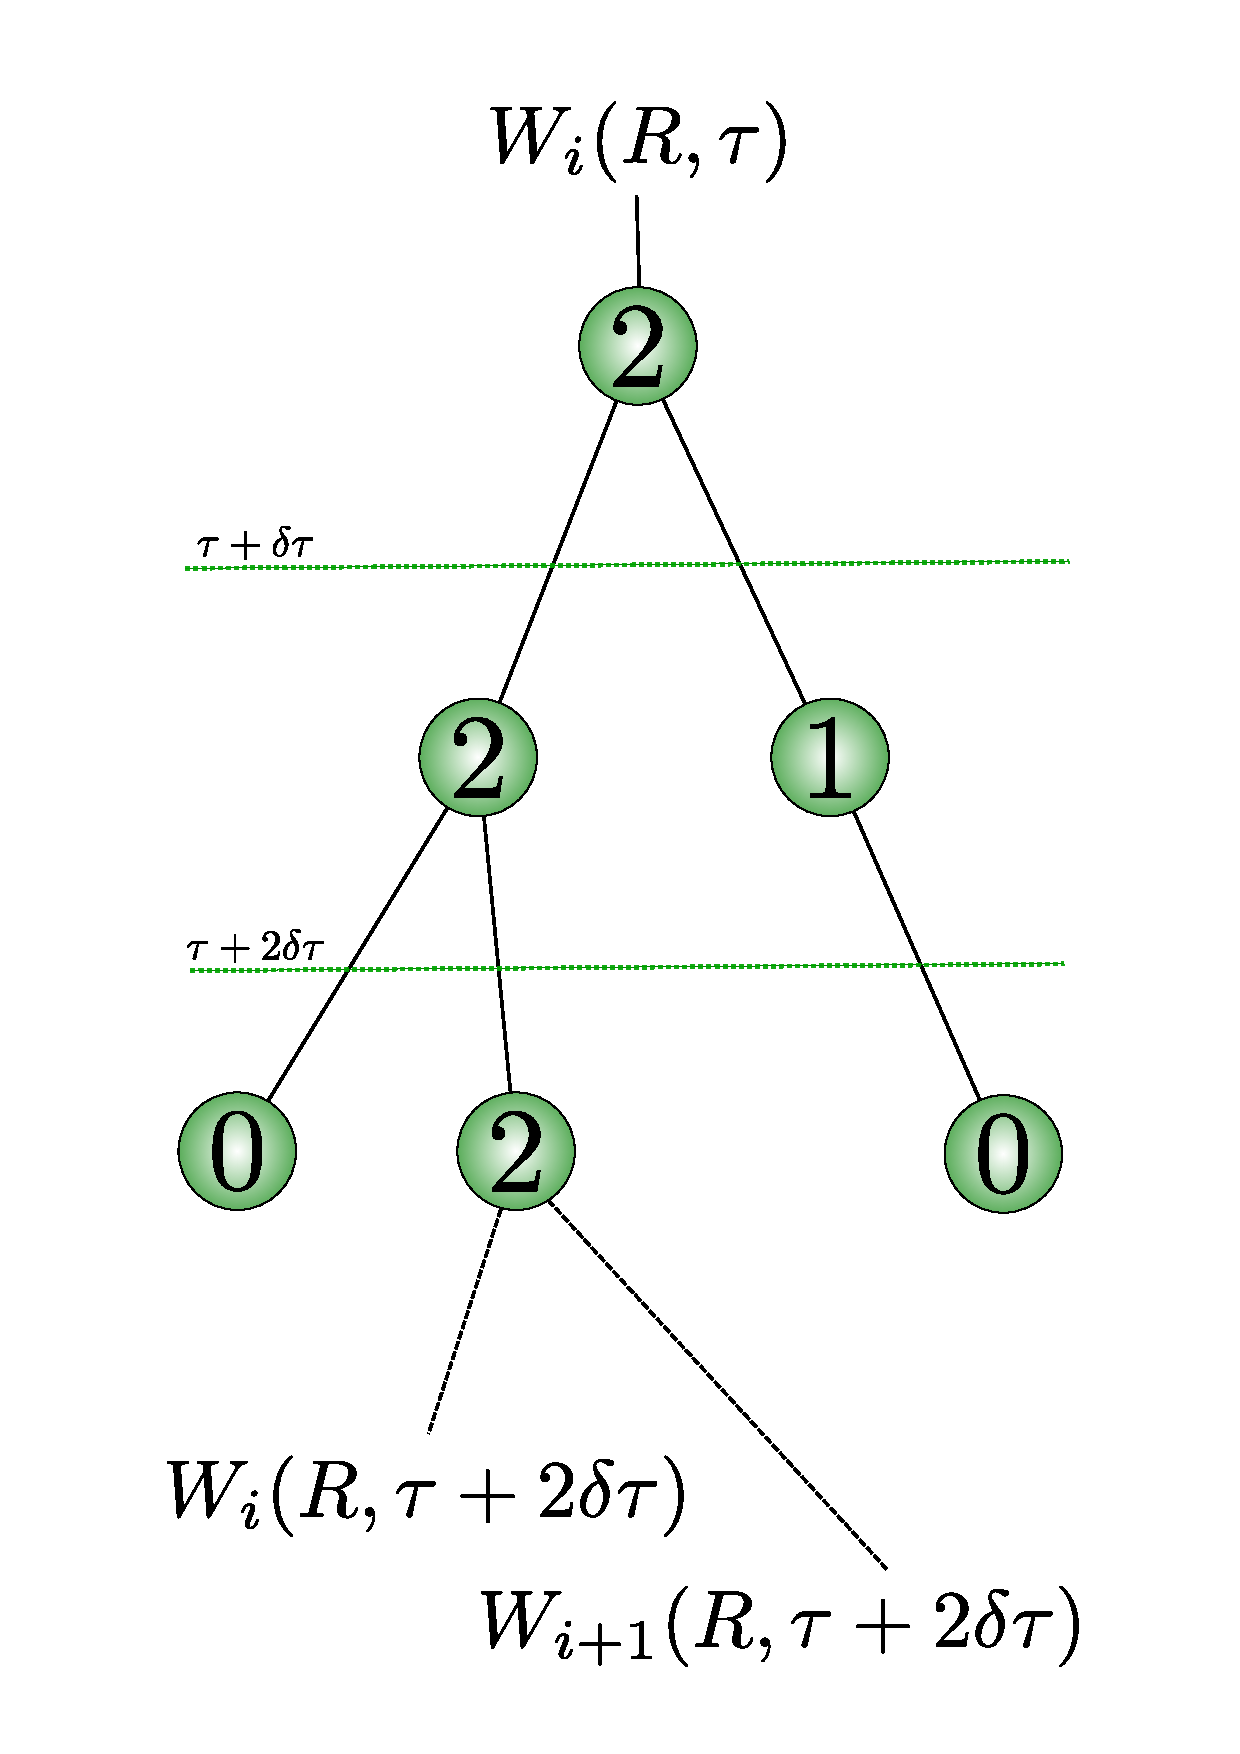
\includegraphics[scale=0.5]{../Graphics/branching.pdf}
  \caption{The process of branching illustrated. The initial walker $W_i(R, \tau)$ is branched according to the rules of Section \ref{sec:branching}. The numerical value inside the nodes represents the value of $\overline{G}_B$ from Eq.~(\ref{eq:gbMean}). Each horizontal dashed line represent a diffusion step, i.e.~a transition in time. Two lines exiting the same node represent identical walkers. After moving through the diffusion process, no two walkers should ever be equal, given that not all of the steps was rejected by the Metropolis test.}
  \label{fig:branching}
 \end{center}
\end{figure}
\clearpage

\section{The Trial Wave Function}
\label{sec:trialWF}

The initial condition of the QMC calculations, that is, the trial wave function $\PT$, can in principle be chosen to be any normalizable wave function whose overlap with the exact ground state wave function, $\Psi_0(\mathbf{r})$, is non-zero. 

If the overlap is zero, that is, if $C_0=0$ in Eq.~(\ref{eq:ExactProjection}), the formalism breaks down, and no final state of convergence can be reached. On the other hand, the opposite scenario implies the opposite behavior; the closer $C_0$ is to unity, the more rapidly the exact ground state, $\Psi_0(\mathbf{r})$, will become the dominant contribution to the distribution. 

In other words, the trial wave function should be chosen in such a way that the overlap is optimized, i.e.~close to unity. Since the exact ground state is unknown, this overlap has to be optimized based on educated guesses and by forcing known properties of the exact ground state into the approximation. This will be the focus in this section.  

Before getting into specifics, a few notes on many-body theory is needed. From this point on, all particles are assumed to be identical. For more information regarding Quantum Mechanical concepts and many-body theory, see for example Refs. \cite{griffiths, Sakurai:94, Shavitt}. 

\subsection{Many-body Wave Functions}
\label{sec:manyBodyWFs}

Many-body theory arise from the existence of \textit{many-body interactions}, which in this thesis will be truncated at the level of the Coulomb interaction, that is, the two-body interaction. Nature operates using  $N$-body interactions, however, it is overall safe to assume that the contributions beyond Coulomb decrease as the order of the interactions increase. If only one-body interactions were present, as is the case for non-interacting particles, the full system would decouple into $N$ single particle systems, rendering many-body theory redundant.

Finding the ground state is, not surprisingly, equivalent to solving the time-independent Schrödinger Equation from Eq.~(\ref{eq:schrodTimeIndie}) for the lowest energy eigenvalue, that is

\begin{equation}
 \OP{H}\Psi_0(\mathbf{r}) = E_0\Psi_0(\mathbf{r}),
 \end{equation}
 
where $\mathbf{r} \equiv \{\mathbf{r}_1, \mathbf{r}_2, ..., \mathbf{r}_N\}$ represents the position of every particle. Exact solutions to realistic many-body systems rarely exist, however, like in Section \ref{sec:statingDiff}, expanding the solution in a known basis $\Phi_k(\mathbf{r})$ is always legal, which reduces the problem into that of a \textit{coefficient hunt} 

\begin{equation}
\label{eq:manyBodyExp}
 \Psi_0(\mathbf{r}) = \sum_{k=0}^\infty C_k'\Phi_k(\mathbf{r}),
\end{equation}

where the primed coefficients should not to be confused with the previous coefficients expanding an arbitrary state in the $\Psi_i(\mathbf{r})$ basis (see Eq.~(\ref{eq:schrodGeneralSolution2})). Different many-body methods give rise to different ways of estimating these coefficients, however, certain concepts are necessarily common, for instance truncating the basis at some level, $K$:

\begin{equation}
 \Psi_0(\mathbf{r}) = \sum_{k=0}^K \tilde{C}_k'\Phi_k(\mathbf{r}), \label{eq:manybodyWFexp}
\end{equation}

where $ \tilde{C}_k' \ne  C_k'$ unless $K$ tends to infinity, however, it is overall safe to assume that the value of the coefficients decrease as $k$ increase. 

The many-body basis elements $\Phi_k(\mathbf{r})$ are constructed using $N$ elements from a basis of single particle wave functions, or \textit{orbitals} for short, where $N$ denotes the total number of particles in the system. In other words, these orbitals, labeled $\phi_n(\mathbf{r}_i)$, combined in different ways give rise to the different many-body wave functions making up the total wave function. The process of calculating basis elements often boils down to an exercise in combinatorics involving combinations of orbitals.

To bring some clarity to the relation between the different wave functions, consider the following example: Imagine electrons surrounding a nucleus, i.e~an atom. A single electron occupying a state with quantum number $n$ at a position $\mathbf{r}_i$ is then described by the orbital $\phi_n(\mathbf{r}_i)$. Each unique\footnote{Two wave functions are considered equal if they differ by nothing but a phase factor.} configuration of electrons (in terms of $n$) will give rise to one unique $\Phi_k(\mathbf{r})$. In other words, the complete basis of $\Phi_k(\mathbf{r})$ is described by the collection of all possible excited states and the ground state. $\Phi_0(\mathbf{r})$ is the ground state of the atom, $\Phi_1(\mathbf{r})$ has one electron exited to a higher shell, $\Phi_2(x)$ has another, and so on. See Figure \ref{fig:AtomicOrbitals} for a demonstration of this. The ordering of the terms in Eq.~(\ref{eq:manybodyWFexp}) are thus chosen to represent higher and higher excitations, i.e. the states has higher and higher energy eigenvalues.

\begin{figure}
 \begin{center}
  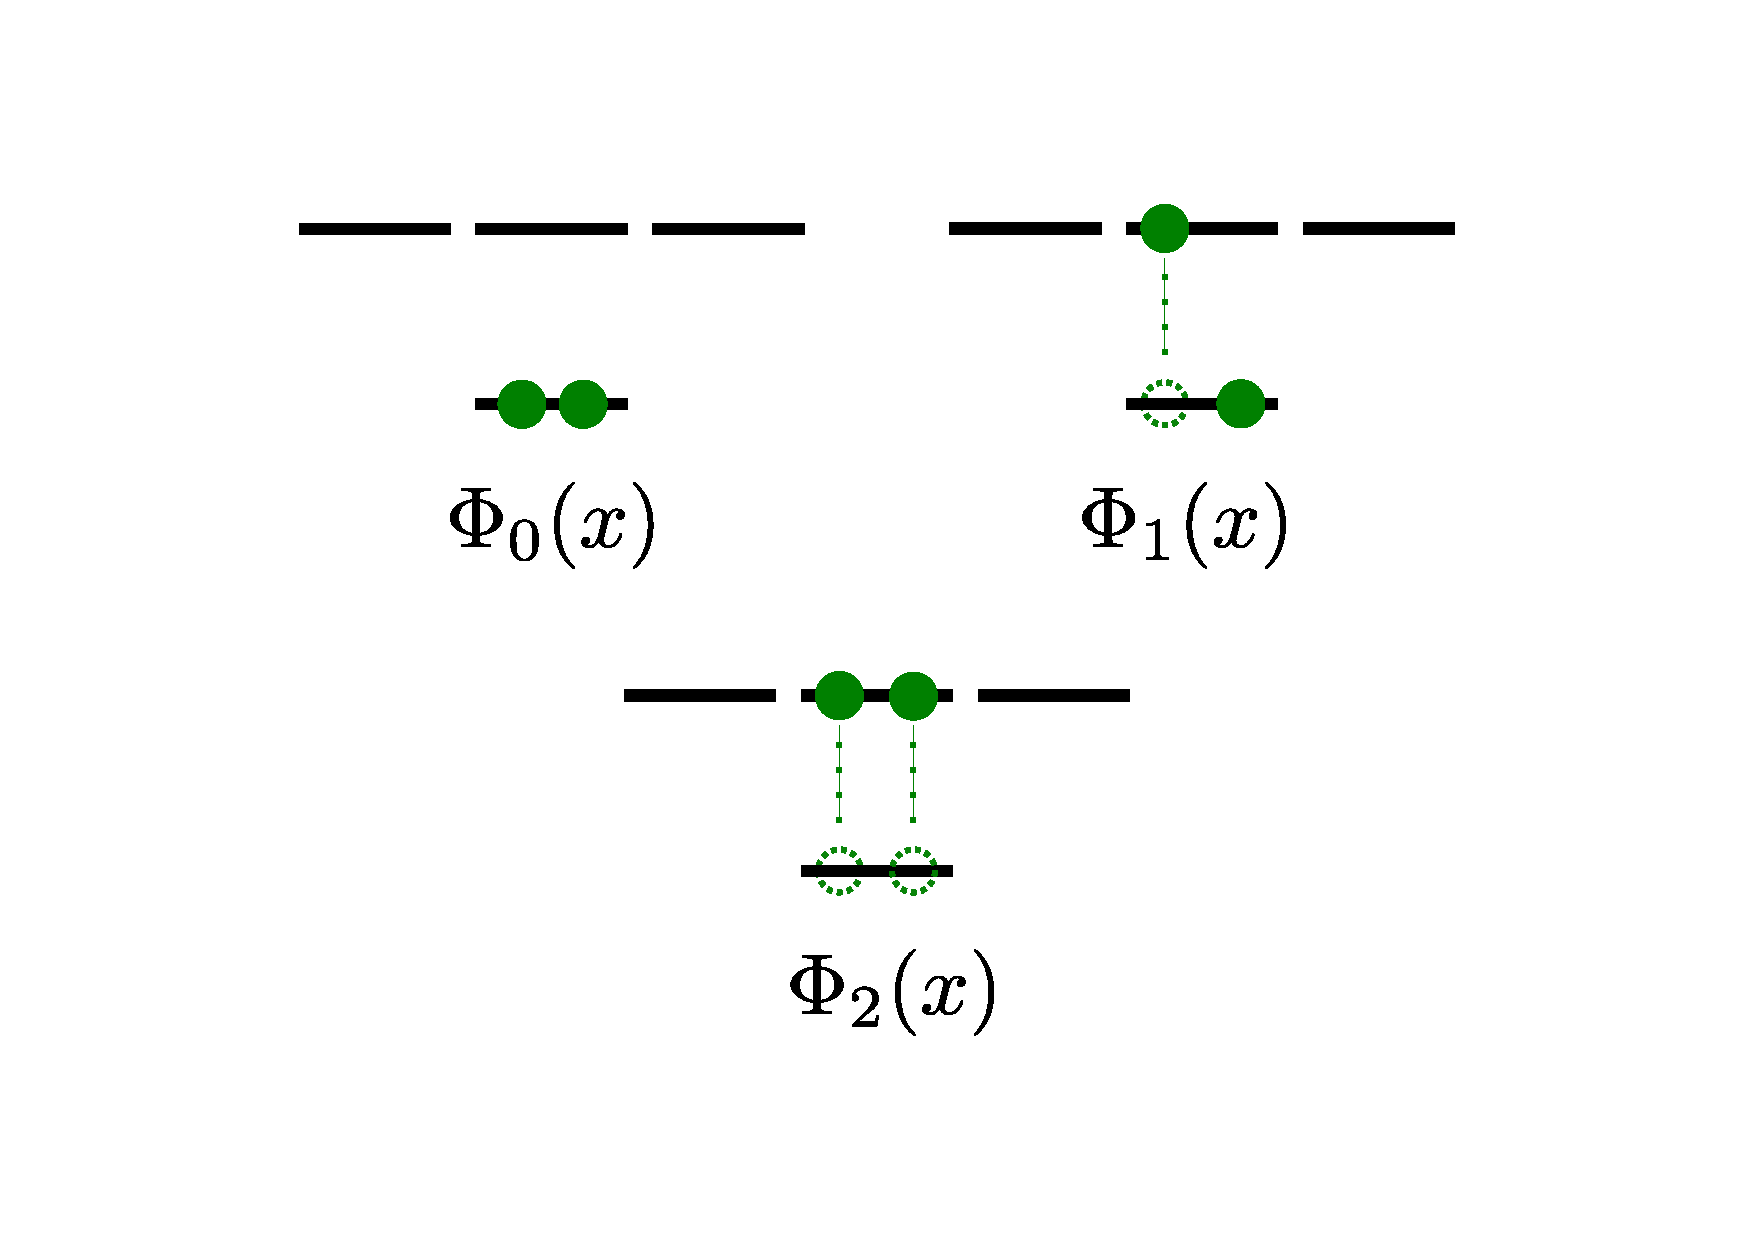
\includegraphics[scale=0.5]{../Graphics/shellStructure.pdf}
  \caption{Three different electron configurations in an shell structure making up three different $\Phi_k(\mathbf{r})$, i.e. constituents of the many-body basis described in Eq.~(\ref{eq:manybodyWFexp}). An electron (solid dot) is represented by e.g. the orbital $\phi_{1s}(\mathbf{r}_1)$.}
  \label{fig:AtomicOrbitals}
 \end{center}
\end{figure}

To summarize, constructing an approximation to an unknown many-body ground state wave function involves three steps:

\begin{center}
\begin{tabular}{l|l}
 \textbf{Step one}   &  Choose a basis of orbitals $\phi_n(\mathbf{r}_i)$, e.g. hydrogen states. \\
 \textbf{Step two}   &  Construct $\Phi_k(\mathbf{r})$ from $N\times$ $\phi_n(\mathbf{r}_i)$.   \\
 \textbf{Step three} &  Construct $\Psi_0(\mathbf{r})$ from $K\times$ $\phi_k(\mathbf{r})$.     \\
\end{tabular}
\end{center}

The last step is well described by Eq.~(\ref{eq:manybodyWFexp}), but is seldom necessary to perform explicitly; expressions involving the approximated ground state wave function is given in terms of the constituent $\Phi_k(\mathbf{r})$ elements and their coefficients.

\subsubsection{Step one in detail}

The Hamiltonian of an $N$-particle system is 

\begin{equation}
 \OP{H} = \OP{H}_0 + \OP{H}_\mathrm{I},
\end{equation}

where $\OP{H}_0$ and $\OP{H}_\mathrm{I}$ are respectively the one-body - and the many-body Hamiltonian. As mentioned in the introduction, the many-body interactions are truncated at the level of the two-body Coulomb interaction. The one-body term consist of the external potential $\OP{u}_\mathrm{ext}(\mathbf{r}_i)$ and the kinetic term $\OP{t}(\mathbf{r}_i)$ for all particles. In order words, the two Hamiltonians are written

\begin{eqnarray}
 \OP{H}_0 &=& \sum_{i=1}^N \OP{h}_0(\mathbf{r}_i) \\
          &=& \sum_{i=1}^N \OP{t}(\mathbf{r}_i) + \OP{u}_\mathrm{ext}(\mathbf{r}_i), \nonumber
  \end{eqnarray}
  and
\begin{eqnarray}
 \OP{H}_\mathrm{I} &\simeq& \sum_{i<j=1}^N \OP{v}(r_{ij}) \\
          &=& \sum_{i<j=1}^N \frac{1}{r_{ij}},  \nonumber
\end{eqnarray}

where $r_{ij} = |\mathbf{r}_i - \mathbf{r}_j|$ is the distance between two particles.

In order to optimize the overlap $C_0$ with the exact wave function, the single particle orbitals are commonly chosen to be the eigenfunctions of the non-interacting single particle Hamiltonian, that is

\begin{equation}
\label{eq:orbitalEigenEq}
 \OP{h}_0(\mathbf{r}_i)\phi_n(\mathbf{r}_i) = \epsilon_n\phi_n(\mathbf{r}_i).
\end{equation}

If no such choice can be made, choosing, free-particle solutions, Laguerre polynomials, or similar, is the general strategy. However, for these bases, the expansion truncation $K$ from Eq.~(\ref{eq:manybodyWFexp}) needs to be higher in order to achieve a satisfying overlap.  


\subsubsection{Step two in detail}

In the case of \textit{fermions}, that is, half-integer spin particles like electrons, protons, etc., $\Phi_k(\mathbf{r})$ is an anti-symmetric function\footnote{Interchanging two particles in an anti-symmetric wave function will reproduce the state changing only the sign.} on the form of a determinant: The so-called \textit{Slater determinant}. The shape of the determinant is given in Eq.~(\ref{eq:SlaterDeterminantExplicit}). The anti-symmetry is a direct consequence of the \textit{Pauli Exclusion Principle}: At any given time, two fermions cannot occupy the same state. 

Bosons, on the other hand, have symmetric wave functions, which in many ways are easier to deal with because of the lack of an exclusion principle. The bosonic many-body wave function is given in Eq.~(\ref{eq:BosonicWFExplicit}). In order to keep the terminology less abstract and confusing, the focus will be on systems of fermions from here on.

\cfbox{1.2cm-6pt}{
\begin{eqnarray}
\label{eq:SlaterDeterminantExplicit}
\Phi_0^\mathrm{AS}(\mbf{r}_1, \mbf{r}_2, ..., \mbf{r}_N) &\propto& \sum_\mathrm{P} (-)^\mathrm{P} \OP{P}\phi_1(\mbf{r}_1)\phi_2(\mbf{r}_2)\,...\,\phi_N(\mbf{r}_N) \nonumber\\
\nonumber\\
&=&\left| \begin{array}{cccc}
\phi_1(\mbf{r}_1) & \phi_2(\mbf{r}_1)& \cdots & \phi_N(\mbf{r}_1) \\
\phi_1(\mbf{r}_2) & \phi_2(\mbf{r}_2)& \cdots & \phi_N(\mbf{r}_2) \\
\vdots & \vdots& \ddots & \vdots \\
\phi_1(\mbf{r}_N) & \phi_2(\mbf{r}_N)& \cdots & \phi_N(\mbf{r}_N) \\
 \end{array} \right|, \\
\nonumber\\
\nonumber\\
 \label{eq:BosonicWFExplicit}
 \Phi_0^\mathrm{S}(\mbf{r}_1, \mbf{r}_2, ..., \mbf{r}_N) &\propto& \sum_\mathrm{P} \OP{P}\phi_1(\mbf{r}_1)\phi_2(\mbf{r}_2)\,...\,\phi_N(\mbf{r}_N).
\end{eqnarray}
}

The permutation operator $\OP{P}$ is simply a way of writing \textit{in any combination of particles and states}, hence the combinatoric exercise mentioned previously. Any combination of $N$ orbital elements $\phi_n(\mbf{r}_i)$ can be used to produce different $\Phi_k(\mathbf{r})$. For illustrative purposes, and for the purpose of this thesis in general where a single determinant ansatz is used, only the ground state has been presented.  

\subsubsection{Dealing with correlations}

The contributions to the ground state on the right-hand side in Eq.~(\ref{eq:manyBodyExp}) for $k>0$ are referred to as \textit{correlation} terms. Given that the single particle wave functions are chosen by Eq.~(\ref{eq:orbitalEigenEq}), the existence of the correlation terms, i.e.~$C_k' \ne 0$ for $k>0$, follows as a direct consequence of the electron-electron interaction, hence the name.

As an example, imagine performing an energy calculation with two particles being infinitely close; the Coulomb singularity will cause the energy to blow up. However, if the calculations are performed using the exact wave function, the diverging terms will cancel out; the energy eigenvalue is independent of the position of the state. 

In other words, a necessary property of the exact wave function is that the singularities in the many-body interactions are canceled. The basic idea is thus to make sure the trial wave function also has this property. By doing so, it is brought closer to the exact wave function.

These criteria are called \textit{cusp conditions} \cite{morten}, and serve as powerful guides when it comes to selecting an optimal trial wave function. 


\subsection{Choosing the Trial Wave Function}
\label{sec:ChoiceTrialWF}

To recap, choosing the trial wave function boils down to optimizing the overlap $C_0 = \braket{\Psi_0}{\Psi_T}$ using a priori knowledge about the system at hand. As discussed previously, the optimal choice of single particle basis is the eigenfunctions of the non-interacting case (given that they exist). Starting from Eq.~(\ref{eq:manybodyWFexp}), from here on referred to as the \textit{spatial wave function}, the first step is to make sure the cusp conditions are obeyed.

Introducing the correlation functions $f(r_{ij})$, where $r_{ij}$ is the relative distance between particle $i$ and $j$, the general ansatz for the trial wave function becomes

\begin{equation}
\label{eq:firstAnzatsTWF}
 \Psi_T(\mbf{r}_1, ..., \mbf{r}_N) = \Big[\sum_{k=0}^K C_k\Phi_k(\mbf{r}_1, ..., \mbf{r}_N)\Big]\prod_{i<j}^Nf(r_{ij}).
\end{equation}

The idea is now to choose $f(r_{ij})$ in such a way that the cusp conditions are obeyed. This should, in light of previous discussions, reduce the amount of terms needed in the spatial wave function to obtain a satisfying overlap.

\subsubsection{Explicit shapes}

Several models for the correlation function exist, however, some are less practical than others. An example given in ref. \cite{abInitioMC} demonstrates this nicely: Hylleraas presented the following correlation function 

\begin{equation}
 f(r_{ij})_\mathrm{Hylleraas} = e^{-\frac{1}{2} (r_i + r_j)}\sum_k d_k(r_{ij})^{a_k} (r_i + r_j)^{b_k}(r_i - r_j)^{e_k},
\end{equation}

where all $k$-subscripted parameters are free. Calculating the helium ground state energy using this correlation function with nine terms yields a four decimal precision. Eight digit precision is achieved by including 1078 terms. For the purpose of QMC, including such vast amounts of parameters is out of the question. The strength of QMC is that very good results can be obtained using a very simple ansatz to the wave function. 

A commonly used correlation function in studies involving few variational parameters is the \textit{Padé Jastrow} function

\begin{eqnarray*}
 \prod_{i<j}^Nf(r_{ij}) &=& \exp(U), \\
         U &=&  \sum_{i<j}^N\left(\frac{\sum_k a_kr_{ij}^k}{1 + \sum_k \beta_kr_{ij}^k}\right) + \sum_i^N\left(\frac{\sum_k a'_kr_i^k}{1 + \sum_k \alpha_kr_i^k}\right).
\end{eqnarray*}

For systems where the correlations are relatively well behaved, it is custom to drop the second sum all together, and keep only the $k=1$ term from the first. The resulting function reads

\begin{equation}
 \label{eq:jastrow}
 f(r_{ij}; \beta) = \exp\left(\frac{a_{ij} r_{ij}}{1 + \beta r_{ij}}\right),
\end{equation}

where $\beta$ is a variational parameter, and $a_{k=1} \equiv a_{ij}$ is a constant depending on the relative spin-orientation of particles $i$ and $j$ tuned in such a way that the cusp conditions are obeyed. For three dimensions, $a_{ij} = 1/4$ or $a_{ij} = 1/2$ depending on whether or not the spins of $i$ and $j$ are parallell or anti parallell respectively\cite{abInitioMC}. For two dimensions, the values are $a_{ij}=1/3$ (parallell) or $a_{ij}=1$ (anti-parallel)\cite{larseivind}. This is the correlation function used for all systems in this thesis.

Shifting the focus back to the spatial wave function, in the case of a fermionic system, the evaluation of an $N\times N$ Slater determinant severely limits the efficiency of many-particle simulations. However, assuming the Hamiltonian to be spin-independent, the eigenstates for different spin eigenvalues will be identical. This fact results in the spatial wave function being split in two: One part for each spin eigenvalue. A detailed derivation of this is given in the appendix of Ref. \cite{QMCPHD2008}. The resulting wave function thus becomes

\begin{equation}
 \Psi_T(\mathbf{r}; \beta) = \Big[\sum_{k=0}^K C_k'\tilde\Phi_k(\mbf{r}_1, ..., \mbf{r}_{\frac{N}{2}})\tilde\Phi_k(\mbf{r}_{\frac{N}{2}-1}, ..., \mbf{r}_{N})\Big]\prod_{i<j}^Nf(r_{ij}; \beta). \label{eq:splitSlater}
\end{equation}

Due to the identical nature of the particles, they may be arbitrarily ordered. For simplicity, the first half represents spin up, and the second half spin down. The spin up determinant will from here on be labeled $|\mathbf{S}^\uparrow|$, and the spin down one $|\mathbf{S}^\downarrow|$, where the $\mathbf{S}$ matrix will be referred to as the \textit{Slater matrix}. Stitching everything together, the explicit shape of the trial wave function becomes

\cfbox{1.5cm-8pt}{
\begin{equation}
\label{eq:MultiDeterminantTWF}
 \Psi_T(\mbf{r}_1, ..., \mbf{r}_N; \beta) = \sum_{k=0}^K C_k' |\mathbf{S}^\uparrow|_k|\mathbf{S}^\downarrow|_k\prod_{i<j}^Nf(r_{ij}; \beta).
\end{equation}
}

This shape is referred to as a \textit{multi-determinant} trial wave function unless $K=1$, in which it will be referred to as a \textit{single-determinant} trial wave function.

\subsubsection{Limitations}

Depending on the complexity of the system at hand, more complicated trial wave functions might be needed to obtain reasonable convergence. However, it is important to distinguish between simply integrating a trial wave function, and performing the full diffusion calculation. As a reminder: Simple integration will not be able to alter the distribution; what you have is what you get. Solving the diffusion problem, on the other hand, will alter the distribution from that of the trial wave function ($\tau = 0$) into a distribution closer to the exact wave function by Eq.~(\ref{eq:schrodGeneralSolution2}). 

Because of this fact, limitations due to the trial wave function in full\footnote{``Full'' in the sense that all Green's functions are applied. As will be revealed later, VMC corresponds to a standard importance sampled Monte-Carlo integration by omitting the branching process.} QMC is far less than what is the case of standard Monte-Carlo integration. A more complex trial wave function might convergence faster, but at the expense of being more CPU-intensive. This implies that CPU-time per walker can be traded for convergence time. For systems of many particles, the CPU-time per walker needs to be as low as possible in order to get the computation done in a reasonable amount of time. In other words, the choice of trial wave function needs to be done in light of the system at hand, and the specific aim of the computation. 

On the other hand, when the number of particles in the system increase, it is safe to assume that the quality of the trial wave function will decrease. This is demonstrated in Ref. \cite{UmrigarMolecules}, where calculations for $\mathrm{F}_2$ (18 particles) need an increase in the number of determinants to achieve a result with the same precision as calculations for $\mathrm{O}_2$ (16 particles).  

\subsubsection{Single-determinant trial wave functions}

In the case of well-behaving systems, a single determinant with a simple Jastrow factor serves as a reasonable trial wave function. This simplicity opens up the possibility of simulating large systems efficiently.  More details regarding this will be given in Section \ref{sec:optSingleSlater}. 

In order to further optimize the overlap with the exact wave function, a second variational parameter $\alpha$ is introduced in the spatial wave function

\cfbox{8mm}{
\begin{equation}
\label{eq:singleDeterminantTWF}
 \Psi_T(\mbf{r}_1, ..., \mbf{r}_N; \alpha, \beta) = D^\uparrow(\alpha)D^\downarrow(\alpha)\prod_{i<j}^Nf(r_{ij}; \beta).
\end{equation}
}

Determining the optimal values of the variational parameters will be the topic of the next section. If the introduction of the variational parameter was redundant, optimizations would simply yield $\alpha=1$. 


\subsection{Selecting Optimal Variational Parameters}
\label{sec:selectingOptVarPar}

All practical ways of determining the optimal values of the variational parameters originate from the same powerful principle: \textit{The Variational Principle}. The easiest way of demonstrating the principle is to evaluate the expectation value of the energy, using an approach similar to what used in Eq.~(\ref{eq:schrodGeneralSolution2}). Consider the following relations

\begin{eqnarray*}
 E_k &=& \bra{\Psi_k}\OP{H}\ket{\Psi_k},  \\
 E   &=& \bra{\Psi_T(\alpha, \beta)}\OP{H}\ket{\Psi_T(\alpha, \beta)}\\
     &=& \sum_{kl} C_k^\ast C_l \underbrace{\bra{\Psi_k}\OP{H}\ket{\Psi_l}}_{E_k\delta_{kl}} \\
     &=& \sum_k |C_k|^2E_k.
\end{eqnarray*}

Just as with the projection operator, introducing $E_k = E_0 + \delta E_k$ where $\delta E_k \ge 0$ will simplify the arguments

\begin{eqnarray*}
 E   &=& \sum_k |C_k^2| (E_0 + \delta E_k) \\
     &=& E_0 \underbrace{\sum_k |C_k^2|}_{1} + \underbrace{\sum_k |C_k|^2\delta E_k}_{\ge 0} \\
     &\ge& E_0.
\end{eqnarray*}

The conclusion is remarkable: No matter which trial wave function is used, the resulting energy will always be greater or equal to the exact ground state energy. This implies that the problem of choosing variational parameters comes down to a minimization problem in the parameters space

\begin{equation}
\label{eq:varMin}
\frac{\partial \langle E\rangle}{\partial \alpha_i} = \frac{\partial}{\partial \alpha_i}\bra{\Psi_T(\alpha_i)}\OP{H}\ket{\Psi_T(\alpha_i)} = 0
\end{equation}

In order to work with Eq.~(\ref{eq:varMin}) in practice, it needs to be rewritten in terms of known values. Since the wave function depends on the variational parameter, the normalization factor needs to be included in the expression of the expectation value. Applying the product rule numerous times yields

\newcommand{\Norm}{\braket{\Psi_T(\alpha_i)}{\Psi_T(\alpha_i)}}

\begin{eqnarray*}
 \frac{\partial \langle E\rangle}{\partial \alpha_i}  &=& \frac{\partial}{\partial \alpha_i} \frac{\bra{\Psi_T(\alpha_i)}\OP{H}\ket{\Psi_T(\alpha_i)}}{\Norm} \\
 &=& \frac{\left(\bra{\Psi_T(\alpha_i)}\frac{\partial}{\partial \alpha_i}\OP{H}\ket{\Psi_T(\alpha_i)} + \bra{\Psi_T(\alpha_i)}\OP{H}\frac{\partial}{\partial \alpha_i}\ket{\Psi_T(\alpha_i)}\right)}{\Norm^2}\Norm \\
 &-& \bra{\Psi_T(\alpha_i)}\OP{H}\ket{\Psi_T(\alpha_i)}\frac{\left(\bra{\Psi_T(\alpha_i)}\frac{\partial}{\partial \alpha_i}\right)\ket{\Psi_T(\alpha_i)} + \bra{\Psi_T(\alpha_i)}\left(\frac{\partial}{\partial \alpha_i}\ket{\Psi_T(\alpha_i)}\right)}{\Norm^2}.\\
\end{eqnarray*}

The Hamiltonian does not depend on the variational parameters, hence both terms in the first expansion is equal. Cleaning up the expression yields

\cfbox{2cm-10pt}{
\begin{eqnarray}
 \frac{\partial \langle E\rangle}{\partial \alpha_i} &=& 2\left(\frac{\bra{\Psi_T(\alpha_i)}\OP{H}\frac{\partial}{\partial \alpha_i}\ket{\Psi_T(\alpha_i)}}{\Norm} - \langle E \rangle\frac{\bra{\Psi_T(\alpha_i)}\frac{\partial}{\partial \alpha_i}\ket{\Psi_T(\alpha_i)}}{\Norm} \right) \nonumber \\
  &=& 2\left(\left< E \frac{\partial \Psi_T}{\partial \alpha_i} \right> -\left< E\right>\left<\frac{\partial \Psi_T}{\partial \alpha_i} \right> \right). \label{eq:varParGrad} \\
  \nonumber
\end{eqnarray}
}

In the case of $\Psi_T(\mathbf{r}; \alpha_i)$ being represented by a Slater determinant, the relationship between the variational derivative of the determinant and the variational derivative of the single particle orbitals $\phi_n(\mathbf{r}_i; \alpha_i)$ is

\cfbox{2cm-5pt}{
\begin{equation}
 \frac{\partial \Psi_T(\mathbf{r}; \alpha_i)}{\partial \alpha_i} = \sum_{p=1}^N\sum_{q=0}^{N/2} \phi_q(\mathbf{r}_p; \alpha_i) \left[\frac{\partial \phi_q(\mathbf{r}_p; \alpha_i)}{\partial \alpha_i}\right]\mathbf{S}^{-1}_{qp},
\end{equation}
}

where $\mathbf{S}^{-1}_{qi}$ is the inverse of the Slater matrix, which will be discussed in more detail in Section \ref{sec:optSlaterRat}. 

Using these expressions for the \textit{variational energy gradient}, the derivatives can be calculated exactly the same way the energy. The gradient can then be used to move in the direction of the variational minimum in Eq.~(\ref{eq:varMin}). 

This strategy gives rise to numerous ways of finding the optimal parameters, such as using the well known Newton's method, conjugate gradient methods \cite{golub1996matrix}, steepest descent (similar to Newton's method), and many more. 
The method implemented for this thesis is called \textit{Adaptive Stochastic Gradient Descent}, and is an efficient iterative algorithm for seeking the variational minimum. The gradient descent methods will be covered in Section \ref{sec:GradientDescent}.

\subsection{Calculating Expectation Values}
\label{sec:calcExpVals}

The expectation value of an operator $\OP{O}$ is obtained by sampling \textit{local} values, $O_L(x)$

\begin{eqnarray}
 \bra{\Psi_T}\OP{O}\ket{\Psi_T} &=& \int \Psi_T(x)^\ast \OP{O} \Psi_T(x)\mathrm{d}x \nonumber\\
                                &=& \int |\Psi_T|^2\left(\frac{1}{\Psi_T(x)}\OP{O}\Psi_T(x)\right)\mathrm{d}x \nonumber\\
                                &=& \int |\Psi_T|^2 O_L(x)\mathrm{d}x. \\
                         O_L(x) &=& \frac{1}{\Psi_T(x)}\OP{O}\Psi_T(x).           
\end{eqnarray}

Discretizing the integral yields 

\begin{equation}
 \bra{\Psi_T}\OP{O}\ket{\Psi_T} \equiv \Exp{O} \simeq \frac{1}{n}\sum_{i=1}^n O_L(x_i) \equiv \overline{O},
\end{equation}

where $x_i$ is a random variable taken from distribution of the trial wave function. The \textit{ensemble average},  $\Exp{O}$ will, given ergodicity, equal the estimated average $\overline{O}$ in the limit $n\rightarrow\infty$, that is

\begin{equation}
 \label{eq:MeanVStrueExp}
 \Exp{O} = \lim_{n\to\infty} \overline{O} = \lim_{n\to\infty}\frac{1}{n}\sum_{i=1}^n O_L(x_i).
\end{equation}


In the case of the energy estimation, this implies that once the walkers reach equilibrium, local values can be sampled based on their configurations $\mathbf{r}_i$ (remember that Metropolis ensures that the walkers follow $|\PT|^2$). In the case of energies, the explicit expression becomes

\begin{equation}
 \langle E \rangle \simeq \frac{1}{n}\sum_{i=1}^n \left(\frac{1}{\Psi_T(\mathbf{r}_i)}\left(-\frac{1}{2}\nabla^2\right)\Psi_T(\mathbf{r}_i) + V(\mathbf{r}_i)\right).
\end{equation}

Incorporating the branching Green's function $G_B$ into the above equation is covered in the DMC section.

\subsection{Normalization}

Every explicit calculation using the trial wave function in QMC involves taking ratios. Calculating ratios implies a cancellation in the normalization factors. Eq.~(\ref{eq:MetroGeneralGreen}) from the Metropolis section, the quantum force in the Fokker-Planck equation, and the sampling of local values described in the previous section demonstrate exactly this; everything involves ratios.

Not having to normalize the wave functions does not only save a lot of CPU-time, but it also removes the need of including the normalization factors of the single particle wave functions; any constants multiplying $\phi_n(x_i)$ in Eq.~(\ref{eq:SlaterDeterminantExplicit}) and Eq.~(\ref{eq:BosonicWFExplicit}) can be taken outside the sum over permutations, and will thus cancel when the ratio between two wave functions constituting of the same single particle orbitals are computed. 

Note, however, that this argument is valid for single determinant wave functions only. 

\section{Gradient Descent Methods}
\label{sec:GradientDescent}

The direction of a gradient serves as a guide to extremal values. Gradient descent, also called steepest descent\footnote{In literature, steepest - and gradient descent are sometimes referred to as being different. However, for simplicity, these will not be differentiated.}, is a family of minimization methods using this property of gradients in order to backtrace a local minimum in the vicinity of an initial guess. 

\subsection{General Gradient Descent}

Seeking maxima or minima is simply a question of whether the positive or the negative direction of the gradient is followed.
Imagine a function $f(x)$, with a minimum residing at $x=x_m$. The information at hand is then

\begin{eqnarray}
 \nabla f(x_m) &=& 0 \\
 \nabla f(x_m - \mathrm{d}x) &<& 0 \\
  \nabla f(x_m + \mathrm{d}x) &>& 0
\end{eqnarray}

where $\mathrm{d}x$ is a infinite decimal displacement. 

\begin{figure}
 \begin{center}
  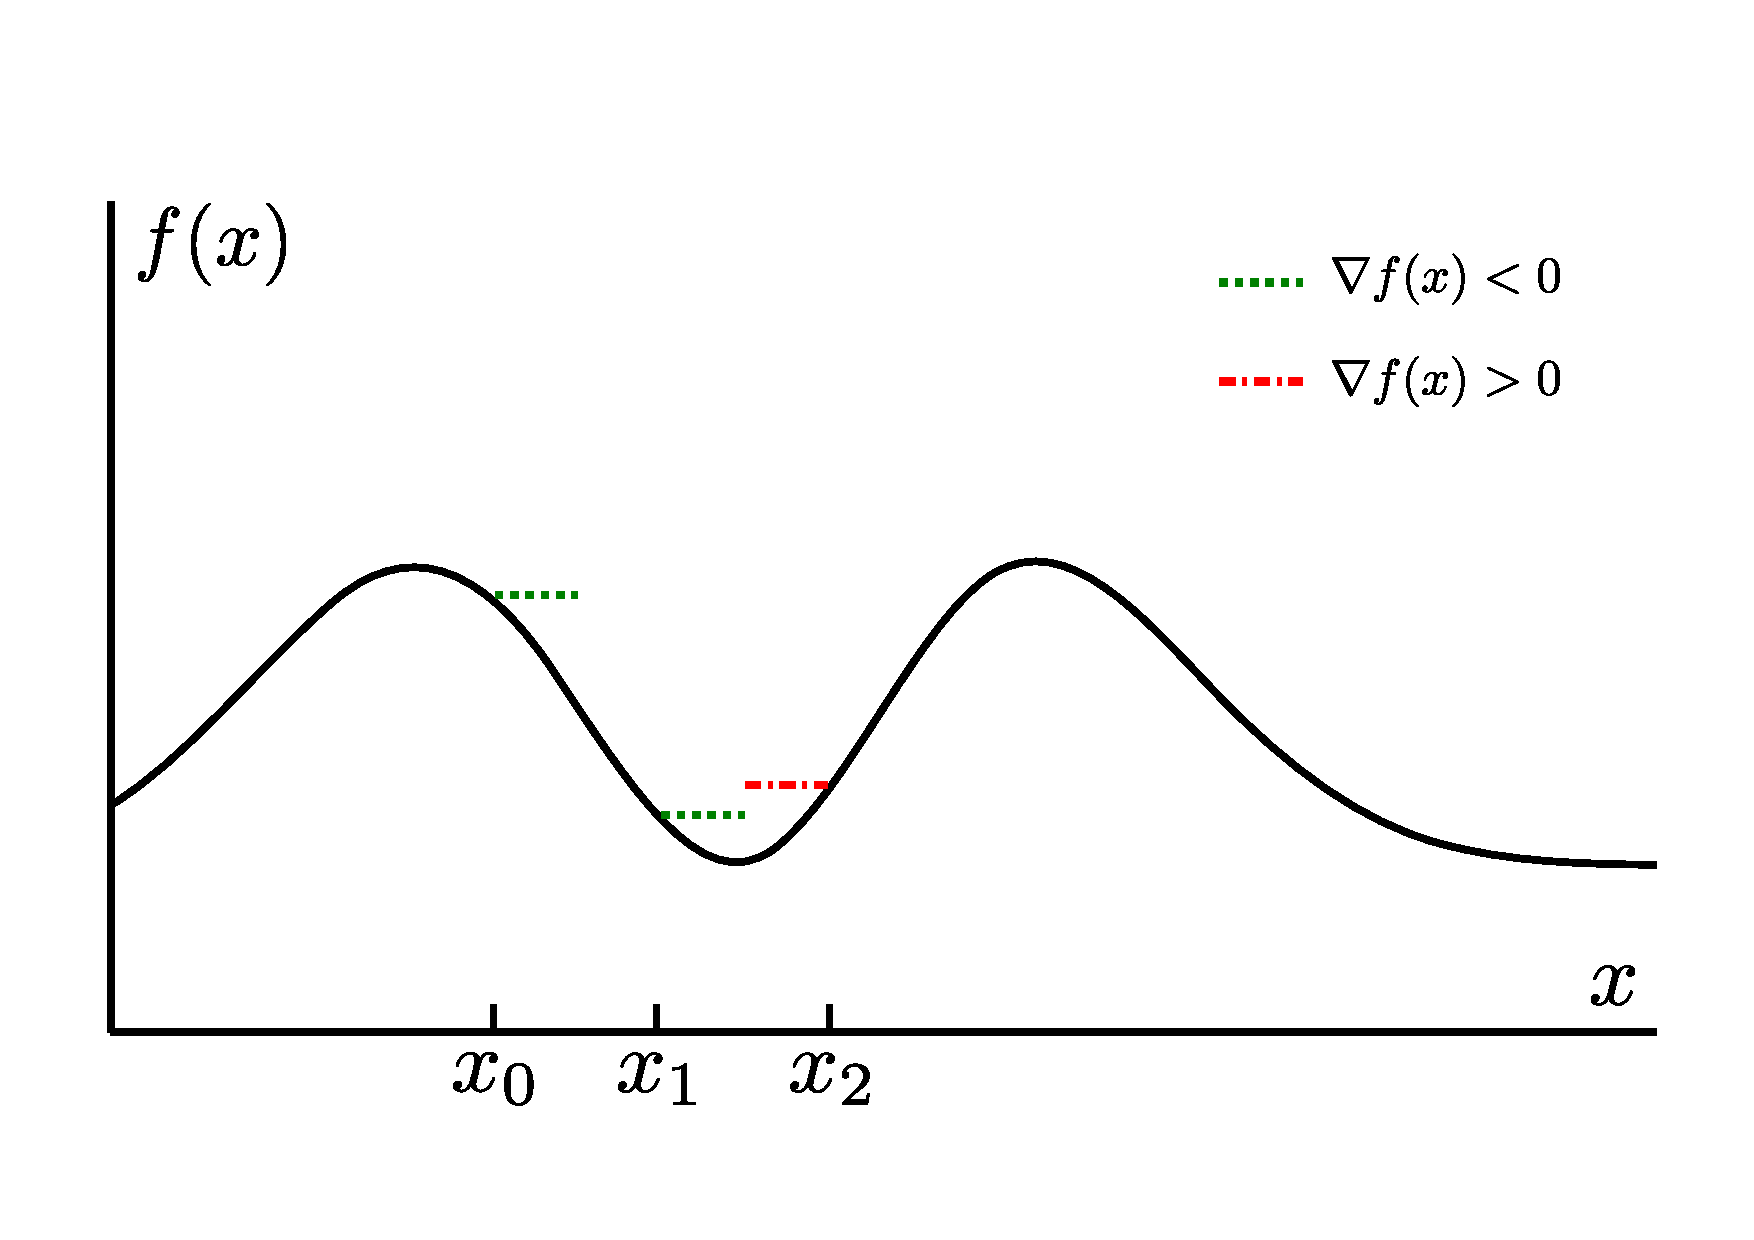
\includegraphics[scale=0.3]{../Graphics/SGD.pdf}
  \caption{Two steps of a one dimensional Gradient Descent process. Steps are taken in the direction of the negative gradient (indicated by dotted lines).}
  \label{fig:SGD}
 \end{center}
\end{figure}

As an example, imagine starting from an initial guess $x_0$. The direction of the gradient is then calculated and followed a number of steps. From Figure \ref{fig:SGD} and the previous equations, it is clear that crossing the true minimum induces a sign change in the gradient. The brute force way of minimizing is to simply end the calculation at this point, however, this would require an extreme amount of very small steps in order to achieve good precision. 

The difference equation describing the steps from the previous paragraph is

\begin{equation}
 x_{i+1} = x_i - \delta\frac{\nabla f(x_i)}{|\nabla f(x_i)|}.
\end{equation}


An improved algorithm would be to continue iterating even though the minimum is crossed, however, this would cause the constant step-length algorithms to oscillate between two points, e.g. $x_1$ and $x_2$ in Figure \ref{fig:SGD}. To counter this, a changing step-length $\delta_i$ is introduced

\cfbox{2.2cm-8pt}{
\begin{equation}
\label{eq:SGD}
  x_{i+1} = x_i - \delta_i\nabla f(x_i).
\end{equation}
}


All gradient/steepest descent methods are in principle described by Eq.~(\ref{eq:SGD})\footnote{This fact sets the perfect scene for an object oriented implementation of gradient descent methods.}. Some examples are

\begin{listliketab}
\storestyleof{itemize}
 \begin{tabular}{l l}
  \textbullet  \,Brute Force I   &  $\delta_i = \delta \frac{1}{|\nabla f(x_i)|}$ \\
  \textbullet  \,Brute Force II  &  $\delta_i = \delta $ \\
  \textbullet  \,Monotone Decreasing &  $\delta_i = \delta / i^{N}$ \\
  \textbullet  \,Newton's Method &  $\delta_i = \frac{1}{\nabla^2 f(x_i)}$\\
 \end{tabular}
\end{listliketab}

Iterative gradient methods will only reveal one local extrema, depending on the choice of $x_0$ and $\delta$. In order to find several extrema, multiple unique processes can be run sequentially or in parallel with different initial guesses.

\subsection{Stochastic Gradient Descent}

Minimizing stochastic quantities such as the variance and expectation values adds another layer of complications on top of the methods introduced in the previous section. Assuming a closed form expression for the stochastic quantity is unobtainable, the gradient needs to be calculated by using e.g.~Monte-Carlo sampling. Eq.~(\ref{eq:varParGrad}) is an example of such a process.

A precise sampling of the stochastic quantities is expensive and unpractical. Stochastic gradient methods use different techniques in order to make the sampling more effective, such as multiple walkers, thermalization, and more. 

Using a finite difference scheme with stochastic quantities is dangerous, as uncertainties in the values will cause the gradient to become unstable when the variations are low close to the minimum. This is illustrated in Figure \ref{fig:sSGD}.

\begin{figure}
 \begin{center}
  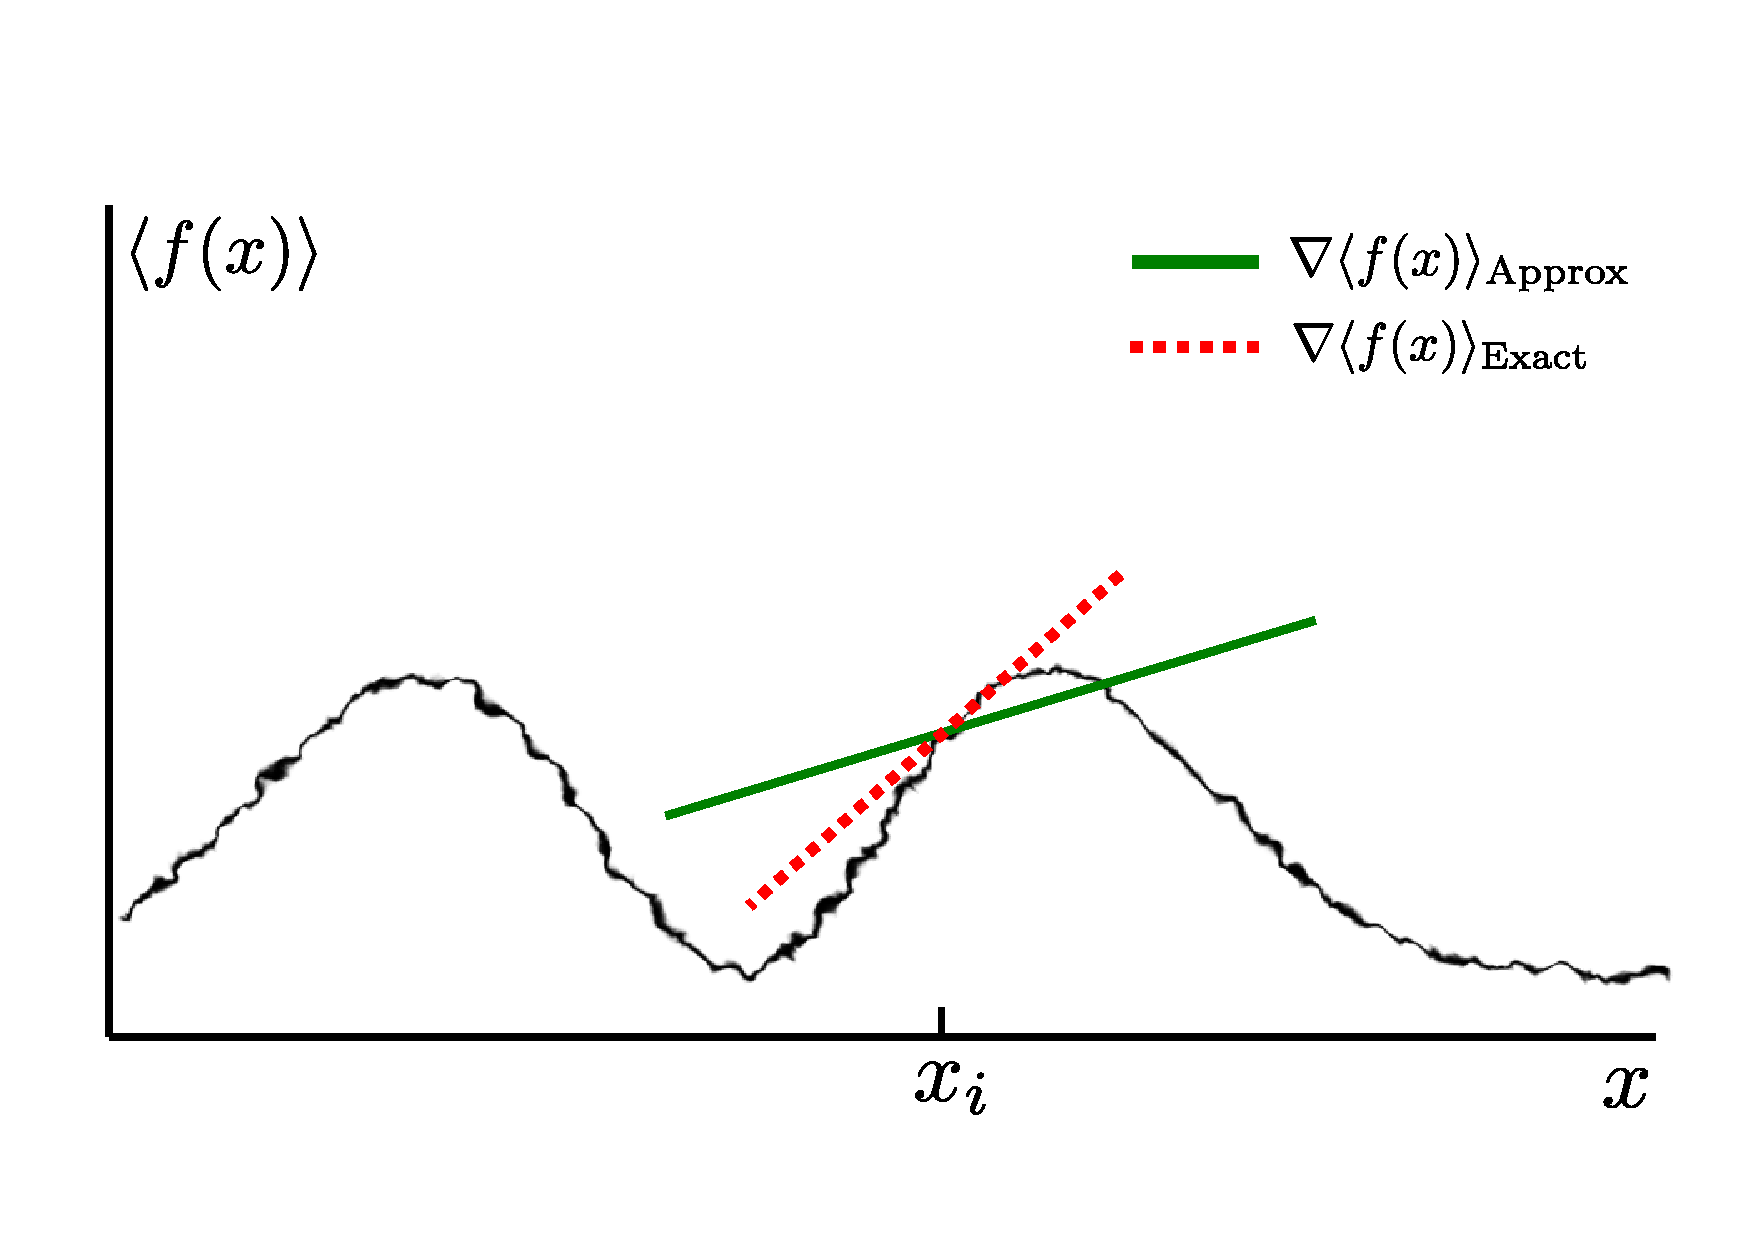
\includegraphics[scale=0.3]{../Graphics/SSGD.pdf}
  \caption{A one dimensional plot of an expectation value function. Smeared lines are representing uncertainties due to rough sampling. The direction of the local gradient (solid green line) at a point $x_i$ is not necessarily a good estimate of the actual analytic gradient (dashed red line).}
  \label{fig:sSGD}
 \end{center}
\end{figure}


\subsection{Adaptive Stochastic Gradient Descent}

Adaptive Stochastic Gradient Descent (ASGD) has its roots in the mathematics of automated control theory \cite{ASGD_MB}. The automated process is that of choosing an optimal step-length $\delta_i$ for the current transition $x_{i}\to x_{i+1}$. This process is based on the inner product of the old and the new gradient though a variable $X_i$

\begin{equation}
\label{eq:ASGD_X_i}
 X_i \equiv -\nabla_i\cdot \nabla_{i-1}.
\end{equation}

The step-length from Eq.~(\ref{eq:SGD}) is modelled in the following manner in ASGD:

\begin{eqnarray}
 \delta_i   &=& \gamma(t_i) \\
 \gamma(t)  &=& a/(t + A) \label{eq:ASGD_delta_i}\\
 t_{i+1}    &=& \max(t_i + f(X_i), 0) \label{eq:ASGD_t_i}\\
 f(x)       &=& f_\mathrm{min} + \frac{f_\mathrm{max} - f_\mathrm{min}}{1 - (f_\mathrm{max}/f_\mathrm{min})e^{-x/\omega}}\label{eq:ASGD_f_i}
\end{eqnarray}

with $f_\mathrm{max} > 0$, $f_\mathrm{min} < 0$, and $\omega > 0$. The free parameters are $a$, $A$ and $t_0$, however, Ref. \cite{ASGD} suggests $A=20$ and $t_0=t_1=A$ for universal usage.

Notice that the step-length increase if $t_i$ decrease and vice-versa. A smaller step-length is sought for regions close to the minimum. The function $f(x)$ is responsible of altering the step-length by changing the trend of $t$. Close to the minimum, a smaller step-length is sought, and hence $t$ must increase. Being close to the minimum implies that the gradient changes sign frequently. Crossing the minimum with ASGD has the following consequence

\begin{itemize}
 \item Eq.~(\ref{eq:ASGD_X_i}): The value of $X_i$ will be positive.
 \item Eq.~(\ref{eq:ASGD_f_i}): $f(X_i)$ will return a value in $[0, f_\mathrm{max}]$ depending on the magnitude of $X_i$.
 \item Eq.~(\ref{eq:ASGD_t_i}): The value of $t$ will increase, i.e. $t_{i+1} > t_i$.
 \item Eq.~(\ref{eq:ASGD_delta_i}): The step-length will decrease.
\end{itemize}

The second step regarding $f(X_i)$ can be visualized in Figure \ref{fig:f_ASGD}.

\begin{figure}
 \begin{center}
  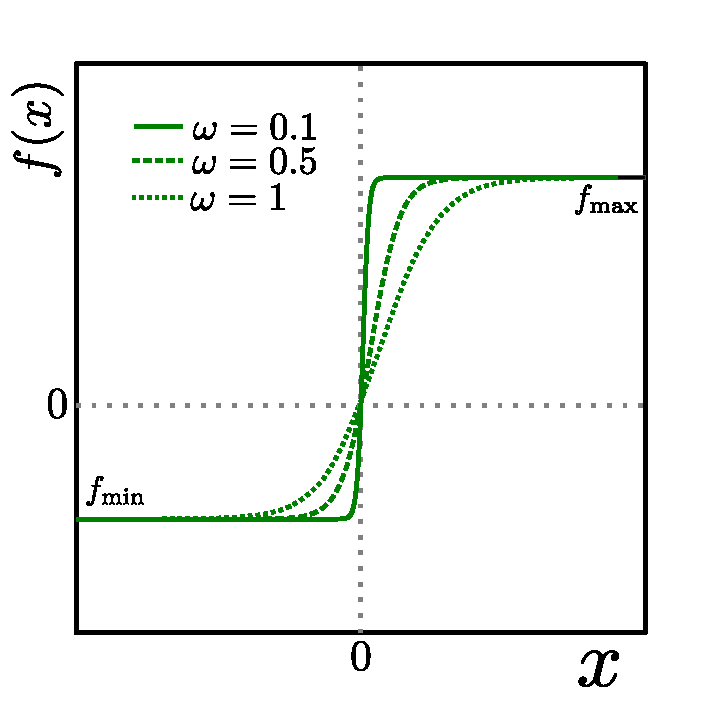
\includegraphics[scale=0.75]{../Graphics/ASGD_f.pdf}
  \caption{Examples of $f(X_i)$ as published in Ref. \cite{ASGD}. As $\omega\to0$, $f(x)$ approaches a step function.}
  \label{fig:f_ASGD}
 \end{center}
\end{figure}

\subsubsection{Assumptions}

These assumptions are selected direct citations from Ref. \cite{ASGD}. They are listed in order to give an impression that the shapes of the functions used in ASGD are not selected at random, but carefully chosen to work optimally in a stochastic space with averages estimated using very few samples.

\begin{itemize}
 \item The statistical error in the sampled gradients are distributed with zero mean.
\end{itemize}

This is shown in Ref. \cite{ASGD}; they are normally distributed. The implication is that upon combining gradient estimates for $N$ different processes, the accumulative error will tend to zero quickly.

\begin{itemize}
 \item The step-length $\gamma(t)$ is a positive monotone decreasing function defined on $[0,\infty)$ with maximum at $t=0$.
\end{itemize}

With $\gamma(t)$ being as in Eq~(\ref{eq:ASGD_delta_i}), this is easily shown.

\begin{itemize}
 \item The function $f(x)$ is continuous and monotone increasing with $f_\mathrm{min} = \displaystyle\lim_{x\to\infty} f(x)$ and $f_\mathrm{max} =  \displaystyle\lim_{x\to-\infty} f(x)$.
\end{itemize}

This is exactly the behavior displayed in Figure \ref{fig:f_ASGD}.

\subsubsection{Implementation}

A flow chart of the implementation is given in Figure \ref{fig:ASGD_flow}. For specific details regarding the implementation, see the documentation of the code in Ref. \cite{libBorealisCode}. An example of minimization using ASGD is given in Figure \ref{fig:ASGD_Ex}. 

\begin{figure}[h]
 \begin{center}
  \subfigure{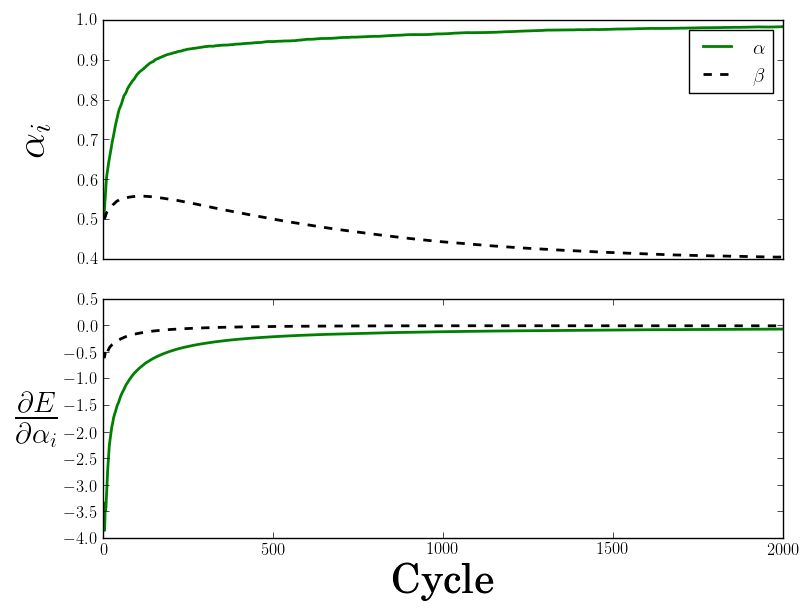
\includegraphics[scale=0.37]{../Graphics/ASGD_min_paramGrad_ex.png}}
  \subfigure{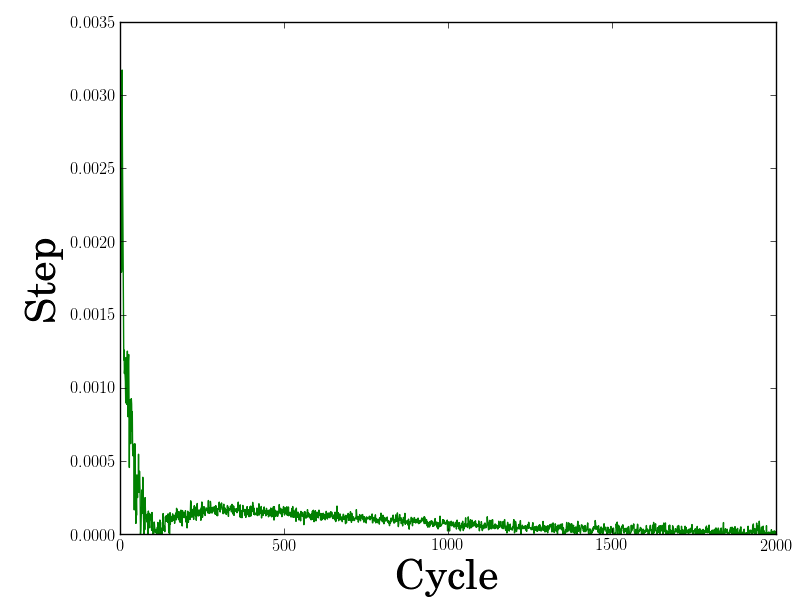
\includegraphics[scale=0.37]{../Graphics/ASGD_min_step_ex.png}} 
  \caption{Results of Adaptive Stochastic Gradient Descent used on a two-particle quantum dot with unit oscillator frequency using $400$ cycles pr. gradient sampling and $40$ independent walkers. The right figure shows the evolution of the time-step. The left figure shows the evolution of the variational parameters $\alpha$ and $\beta$ introduced in Section \ref{sec:trialWF} on top, and the evolution of the gradients on the bottom. The gradients are averaged to reveal the pattern underlying the noise. Dispite this averaging, it is apparent that they tend to zero, $\beta$ somewhat before $\alpha$. The step rushes to zero with a small rebound as it attempts to cross to negative values.}
  \label{fig:ASGD_Ex}
 \end{center}
\end{figure}


\begin{figure}
 \begin{center}
  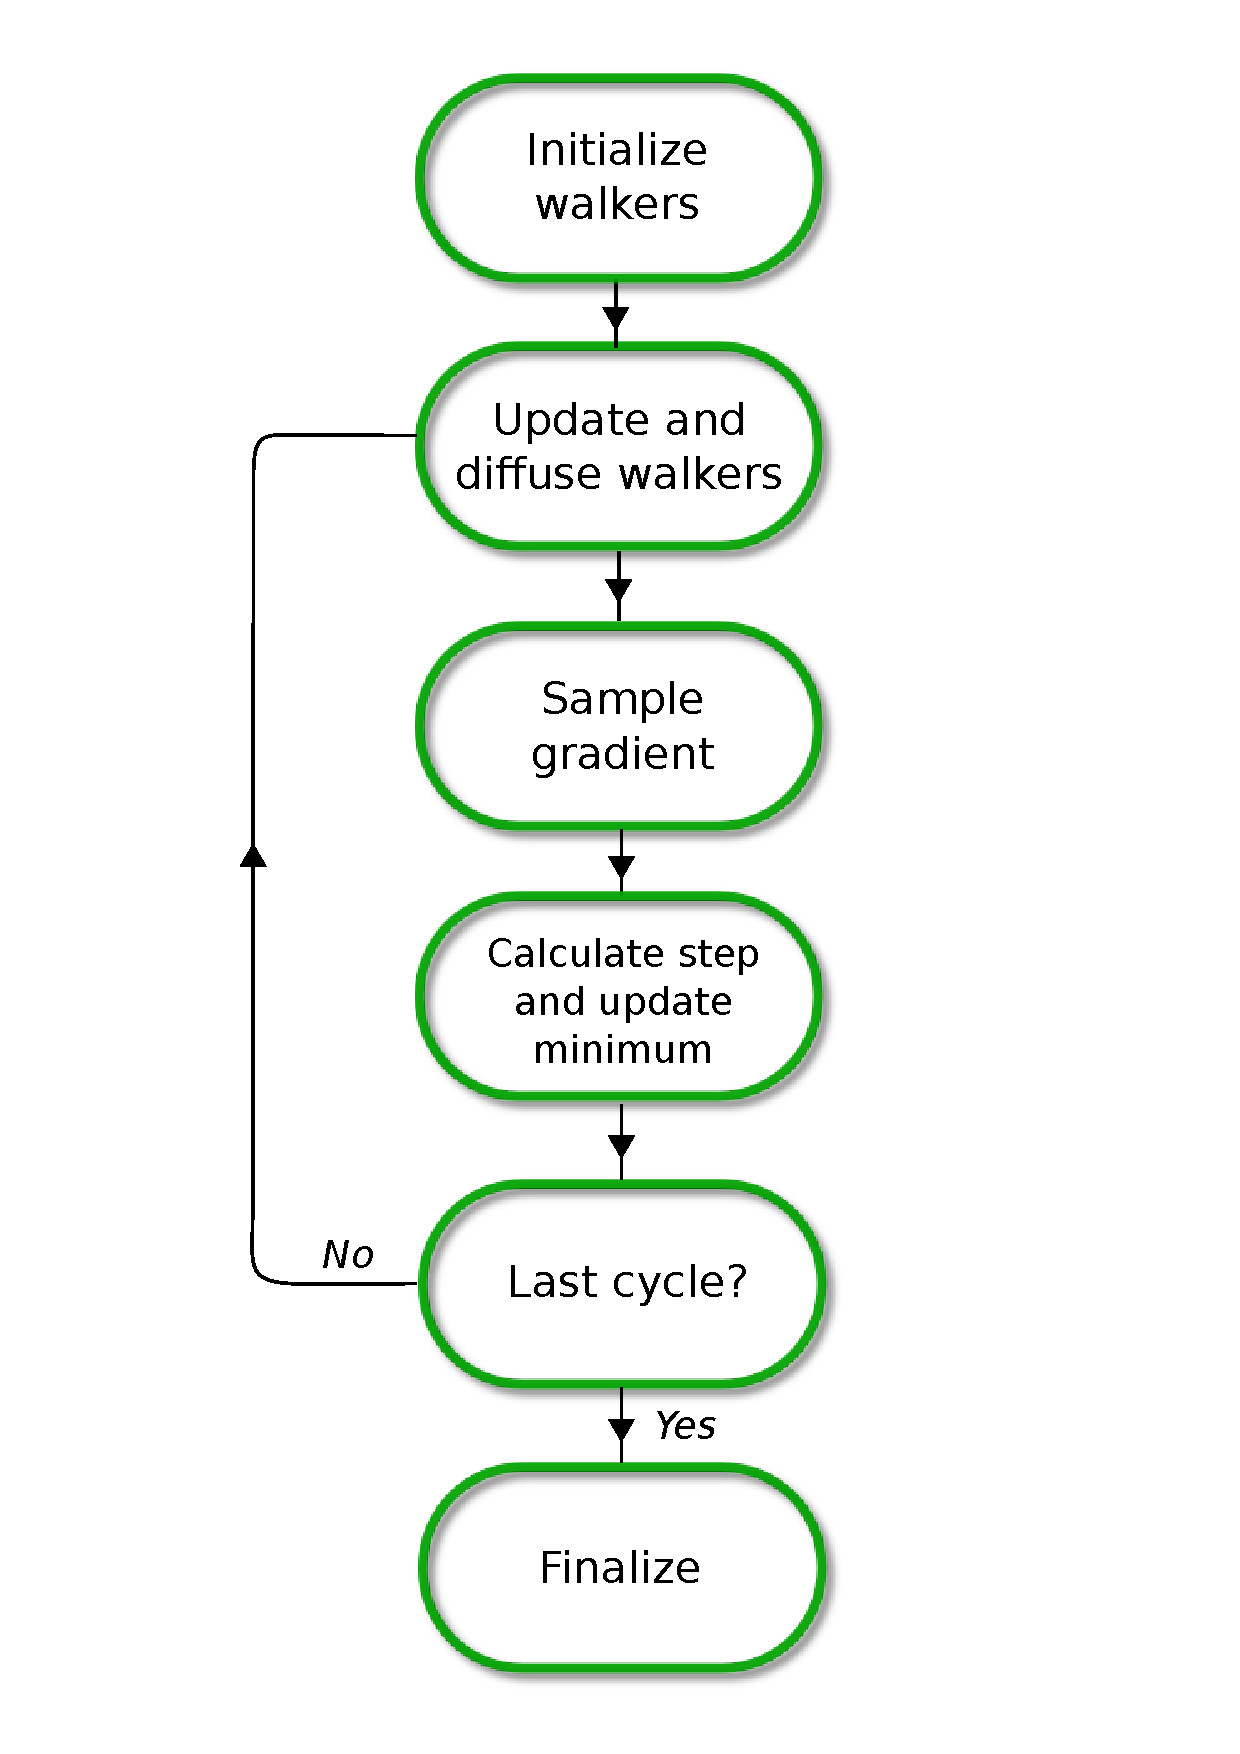
\includegraphics[scale=0.65]{../Graphics/ASGD_UML.pdf}
  \caption{Chart flow of ASGD algorithm. Diffusing a walker is done as described in Figure \ref{fig:diffFlowChart}. Updating the walkers involves recalculating any values affected by updating the minimum. The step is calculated by Eq.~(\ref{eq:ASGD_delta_i}). In the case of QMC, the gradient is sampled by Eq.~(\ref{eq:varParGrad}).}
  \label{fig:ASGD_flow}
 \end{center}
\end{figure}
\clearpage


\section{Variational Monte-Carlo}
\label{sec:VMC}

As briefly mentioned in the Section \ref{sec:statingDiff}, neglecting the branching term, i.e.~setting $G_\mathrm{B}=1$, corresponds to a method called Variational Monte-Carlo (VMC). The name comes from the fact that the method is is variational, that is, it supplies an upper bound to the exact ground state energy. The better the trial wave function is, the closer the VMC energy is to the exact ground state energy.

The converged state of the Markov chain in VMC is controlled by the Metropolis test, and will thus equal the trial wave function squared. From the flow chart of the VMC algorithm in Figure \ref{fig:VMCchart}, it is clear that VMC corresponds to a standard Monte-Carlo integration of the local energy sampled using a distribution equal to the trial wave function squared.

\subsection{Motivating the use of Diffusion Theory}

An important question to answer is why e.g.~the Langevin equation is so important if the result is simply an expectation value. Statistics states that \textit{any} distribution may be used when calculating an expectation value. Why bother with a trial wave function, thermalization, and so on? 

The reason is simple, yet not obvious. The quantity of interest, the local energy, \textit{depends on the trial wave function}. This is demonstrated in the following expression:

\begin{eqnarray}
 E_\mathrm{VMC} &=& \int P(\mathbf{r}) \frac{1}{\PT}\OP{H}\PT\mathrm{d}\mathbf{r} \nonumber\\
                   &\simeq& \frac{1}{n}\sum_{i=1}^n \frac{1}{\Psi_T(\mbf{r}_i)}\OP{H}\Psi_T(\mbf{r}_i), \label{eq:VMCrandomDistE}
\end{eqnarray}

where the points $\mbf{r}_i$ are drawn from the distribution $P(\mathbf{r})$.

Equation (\ref{eq:VMCrandomDistE}) implies that the evaluation of the local energy in an arbitrary distribution $P(\mathbf{r})$ is \textit{undefined} at the zeros of $\PT$. In other words, it is not guaranteed that $P(\mathbf{r})$ does not generate a point $\mathbf{r}_m$ in such a way that $\Psi_T(\mbf{r}_m) = 0$. 

However, if the distribution is chosen as $P(\mathbf{r})=|\PT|^2$, the probability of sampling a point where the local energy is undefined equals zero. This comes as a consequence of the following relation

\begin{equation}
 \Psi_T(\mathbf{r}_m) = 0 \quad\Longrightarrow\quad P(\mathbf{r}_m) = 0
\end{equation}

In other words, the more undefined the energy is at a point, the less probable the point is. This hidden detail is what Quantum Monte-Carlo safely takes care of that standard Monte-Carlo does not. 

\begin{figure}
 \begin{center}
  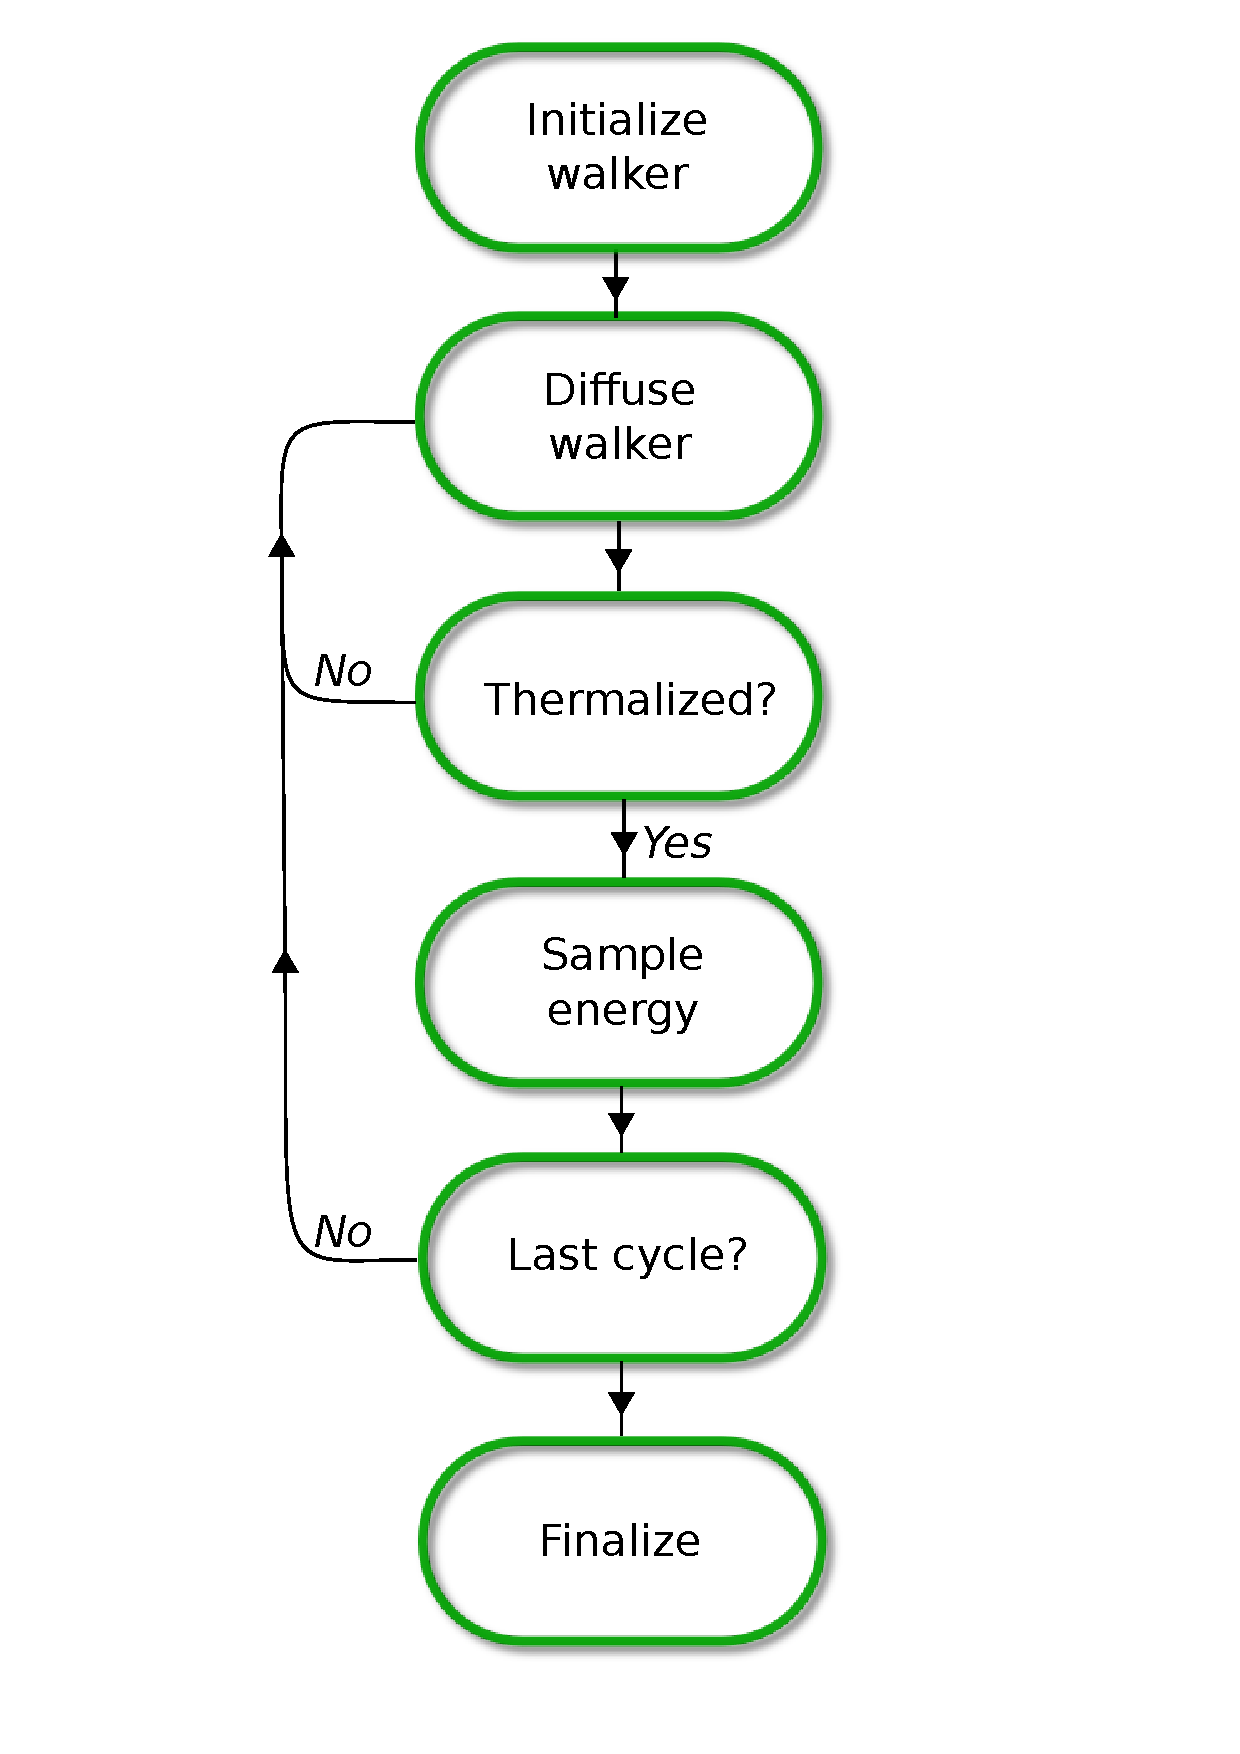
\includegraphics[scale=0.65]{../Graphics/VMCUML.pdf}
  \caption{Chart flow of the Variational Monte-Carlo algorithm. The second step, \textit{Diffuse Walker}, is the process described in Figure \ref{fig:diffFlowChart}. Energies are sampled as described in Section \ref{sec:calcExpVals}. The thermalization is set to a fixed number of cycles. }
  \label{fig:VMCchart}
 \end{center}
\end{figure}
\clearpage

\subsection{Implementation}

Beyond a given point, VMC does not benefit much from an increase of samples. It is much more important that the system is properly thermalized, than using several walkers or many cycles. It is therefore sufficient to use a single walker per VMC simulation.

The single walker is initialized in a normal distributed manner, and released to diffuse according to the process in Figure \ref{fig:diffFlowChart}. After accumulating energies, the final energy is calculated as the mean of these. The process is described in Figure \ref{fig:VMCchart}.

For more details regarding the specific implementation, see the code in Ref. \cite{libBorealisCode}.

\subsection{Limitations}

The only limitation in VMC is the choice of the trial wave function. This makes VMC extremely robust; it will \textit{always} produce a result. As the overlap $C_0$ from Eq.~(\ref{eq:schrodGeneralSolution2}) approach unity, the VMC energy approaches the exact ground state energy as a monotone decreasing function. Figure \ref{fig:VMC_wfcomp} demonstrates this effect. As more optimizations are added to the trial wave function, the lower the VMC energy gets.

\begin{figure}
 \begin{center}
  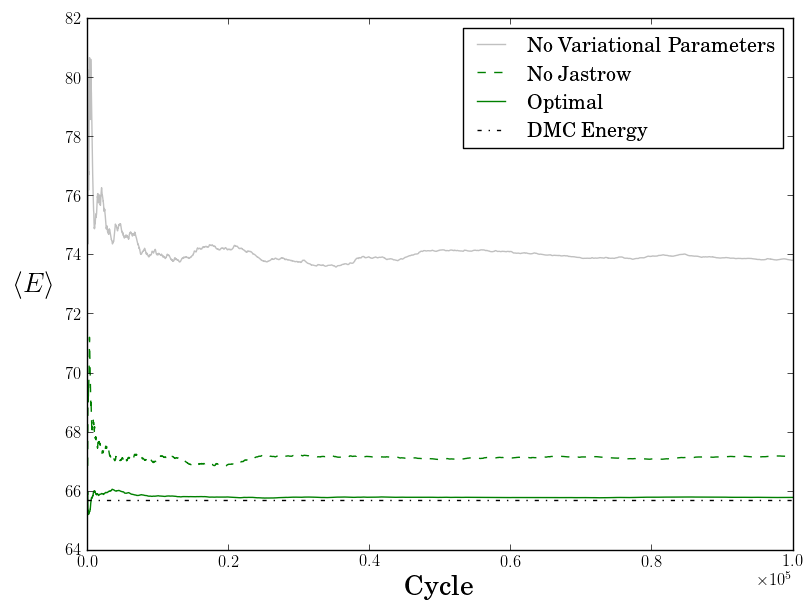
\includegraphics[scale=0.65]{../Graphics/WFComp.png}
  \caption{Comparison of the VMC energy using different trial wave functions. The DMC energy is believed to be very close to the exact ground state. It is apparent that adding a variational parameter to the trial wave function lowers the energy substantially, however, when adding the Jastrow factor (denoted \textit{Optimal}), described in Section \ref{sec:ChoiceTrialWF}, the VMC energy gets very close to the ``exact'' answer. A lower energy means a better energy when dealing with variational methods. In this example, a 12-particle quantum dot with unit frequency is used.}
  \label{fig:VMC_wfcomp}
 \end{center}
\end{figure}

\section{Diffusion Monte-Carlo}
\label{sec:DMC}

Applying the full diffusion framework introduced in Sections \ref{sec:statingDiff} and \ref{sec:solvingDiff} results in a method known as Diffusion Monte-Carlo (DMC)\footnote{In literature, DMC is also known as \textit{Projection Monte-Carlo}, for reasons described in Section \ref{sec:statingDiff}.}. Diffusion Monte-Carlo results are often referred to as \textit{exact}, in the sense that DMC is overall one of the most precise many-body methods available. However, just as any many-body method, DMC also has its limitations. These will be discussed in Section \ref{sec:DMClimitations}.

Where other many-body methods run into the \textit{curse of dimensionality}, that is, the CPU-time scales very bad with increasing number of particles, DMC with its position basis Quantum Monte-Carlo formalism does not. With DMC, it is simply a matter of evaluating a more complicated trial wave function, or simulating for a longer period of cycles, in order to reach convergence to the believed ``exact'' ground state in a satisfactory way.

\subsection{Implementation}

Branching is a major part of the DMC algorithm. Diffusion Monte-Carlo uses a large ensemble of walkers to generate enormous amounts of statistics. These walkers are initialized using a VMC calculation, i.e. the walkers are initially distributed according to the trial wave function squared. 

There are three layers of loops in the DMC method implemented in this thesis, two of which are obvious: The time-step - and walker loops. However, introducing a third \textit{block loop} within the walker loop boosts the convergence dramatically. For each walker, this loop continues until the walker is either dead ($G_B = 0$), or has diffused $n_b$ times. Using this method, ``good'' walkers will have multiple offspring pr cycle, while ``bad'' walkers will rarely survive the block loop. Perfect walkers will supply a ton of statistics as they surf through all the loops without branching ($G_B \sim 1$).

A flow chart of the DMC algorithm is given in Figure \ref{fig:DMCchart}. Comparing it the the corresponding figure for VMC, it is apparent that DMC is by far more complicated. 

\subsection{Sampling the Energy}

As mentioned in Section \ref{sec:statingDiff}, the role of the branching Green's function is to distribute the correct weights to each walker. Each walker's contribution to the cumulative energy sampling should thus be weighed according to the value of the branching Green's function. Let $E_k$ denote the cumulative energy for time-step $\tau = k\delta\tau$, $n_w$ be the number of walkers in the system at time-step $k$, $\tilde n_{b,i}$ be the number of blocks walker $i$ survives, and let $W_i(\mbf{r}, \tau)$ represent walker $i$. The relation is then

\begin{equation}
 E_k = \frac{1}{n_w}\sum_{i=1}^{n_w} \frac{1}{\tilde n_{b,i}}\sum_{l=1}^{\tilde n_{b,i}} G_\mathrm{B}\Big(W_i(\mbf{r}, \tau_k + l\delta\tau)\Big)E_L\Big(W_i(\mbf{r}, \tau_k + l\delta\tau)\Big). \label{eq:DMC_Ek}
\end{equation}

As required, setting $G_B = n_w = n_b = 1$ reproduces the VMC expression. 

The new trial energy from Eq.~(\ref{eq:firstTrialEnergyIntro}) is set equal to the previous cycle's average energy, that is  

\begin{equation}
 E_T = E_k.
\end{equation}

The DMC energy is updated each cycle to be the trailing average of the trial energies:

\cfbox{2.5cm-10pt}{
\begin{equation}
 E_\mathrm{DMC} = \overline{E_T} = \frac{1}{n}\sum_{k=1}^n E_k.
\end{equation}
}


\subsection{Limitations}
\label{sec:DMClimitations}

By introducing the branching term, DMC is a far less robust method compared to VMC. Action must be taken in order to stabilize the iterations through tuning of parameters such as population size, time-step, block size, etc. This is the disadvantage of DMC compared to other many-body methods such as Coupled Cluster \cite{Hirth}, which is far more automatic.

\subsubsection{Time-step errors}

The error introduced by the short time approximation in Eq.~(\ref{eq:shortTimeApprox}) goes as $\mathcal{O}(\delta\tau^2)$. In addition, there is a second error related to the time-step, arising from the fact that not all steps are accepted by the Metropolis algorithm. This introduces a effective reduction in the time-step, and is countered by scaling the time-step with the acceptance ratio upon calculating $G_B$ \cite{abInitioMC}. However, DMC is rarely used without importance sampling, which, due to the quantum force, has an acceptance ratio very close to one. It is therefore common to ignore this problem, as its effect on the final result is minimal.

\subsubsection{Selecting the time-step}

Studying the branching Green's function in equation \ref{eq:branchFP} in more detail reveals that it's magnitude increases exponentially with the spread of the energies $\Delta E$, that is

\begin{equation}
G_B \propto \exp{\left(\Delta E\delta\tau\right)}. 
\end{equation}

As will be shown in Section \ref{sec:varAndSTD}, the spread in energy samples are higher the worse of an approximation to the ground state the trial wave function is. In addition, the magnitude of the spread scales with the magnitude of the energy. 

Setting an upper bound to the branching function might seem like a good idea, however, each time a walker is denied its replicas, an uncontrollable error is introduced in the distribution.

The solution is to balance out the increase in $\Delta E$ by lowering the time-step accordingly. That is

\begin{equation}
 \delta\tau \propto \frac{1}{\Delta E}.
\end{equation}

However, having too low a time-step will hinder DMC from evolving walkers efficiently, especially if the positional span of the distribution is large. In other words, a balance must be found. An indication of whether the time-step was chosen too low or not is obtained by looking at the resulting DMC density. If the density is spiky and disorganized, the time-step was too low. 

Another source of error is due to the \textit{fixed node approximation}. This approximation will be covered in the next section.

\begin{figure}[ht]
 \begin{center}
  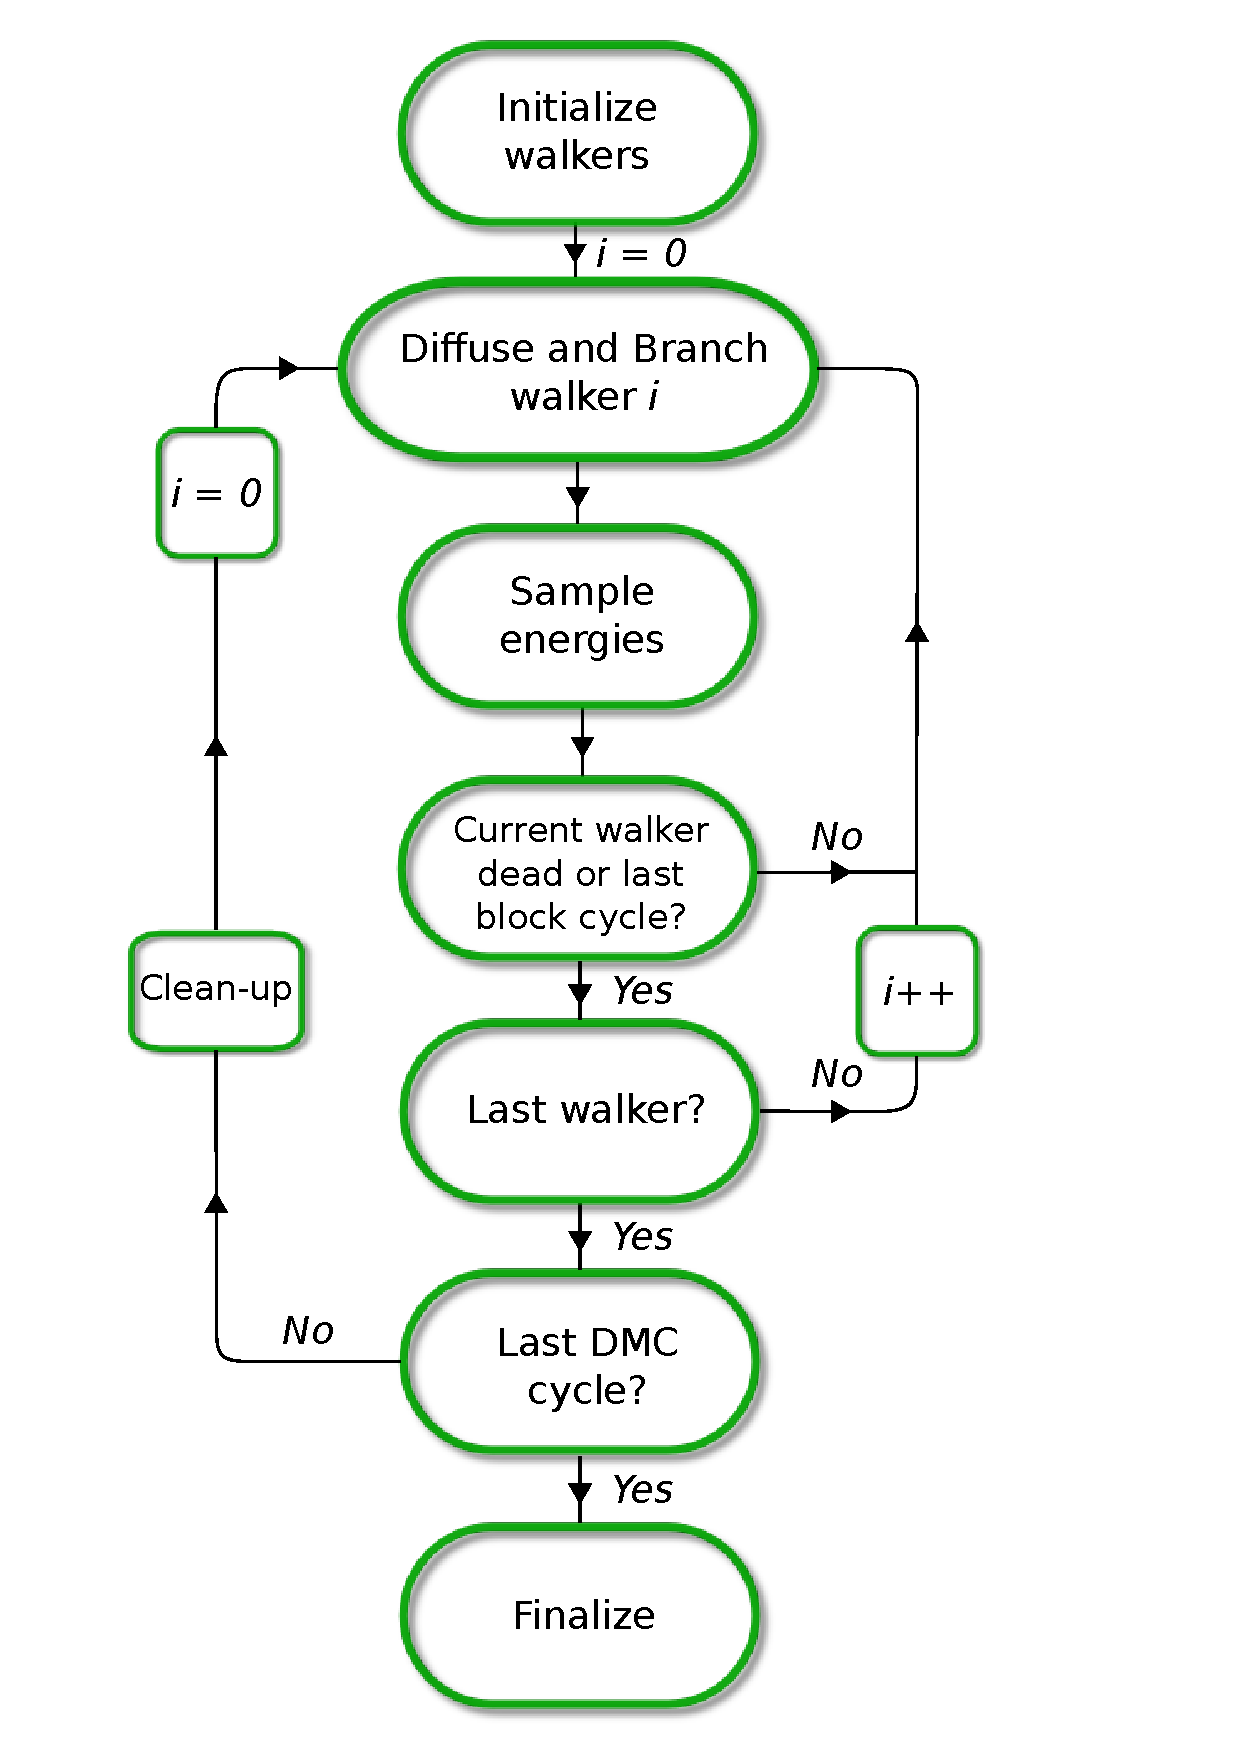
\includegraphics[scale=0.65]{../Graphics/DMCUML.pdf}
  \caption{Chart flow of the Diffusion Monte-Carlo algorithm. The variable \textit{i} represents the currently moved walker. The second step, \textit{Diffuse and Branch Walker}, is the process described in Figure \ref{fig:diffFlowChart} in combination with the branching from Figure \ref{fig:branching}. Energies are sampled as in Eq.~(\ref{eq:DMC_Ek}). Thermalization is set to a fixed number of cycles.}
  \label{fig:DMCchart}
 \end{center}
\end{figure}
\clearpage

\subsection{Fixed node approximation}

Looking at Eq.~(\ref{eq:BosonicWFExplicit}), it is apparent that by choosing positive phases for the single particle wave functions, the bosonic many-body wave function is exclusively positive. For fermions however, the sign change upon interchanging two particles introduces the possibility that the wave function will have both negative and positive regions, independent of the choice of phases in the single particle wave functions.

As DMC iterates, the density of walkers at a given time, $P(\mathbf{r}, \tau)$, represents the projected wave function from Eq.~(\ref{eq:schrodGeneralSolution2}) multiplied by the trial wave function. 

\begin{equation}
 P(\mathbf{r}, \tau) = \Ptau\PT.
\end{equation}

This relationship is described in high detail in Section \ref{sec:anisFokker}.

Applying the projector operator to the distribution yields

\begin{equation}
  \lim_{\tau\to\infty} P(\mathbf{r}, \tau) = \braket{\Phi_0}{\Phi_T}\Phi_0(\mathbf{r})\Psi_T(\mathbf{r}),
\end{equation}

which, if interpreted as a density, should always be greater than zero. In the case of fermions, this is not guaranteed, as
the node structure of the exact ground state and the trial wave function will generally be different.  

To avoid this anomaly in the density, $\Ptau$ and $\PT$ have to change sign simultaneously\footnote{It should be mentioned that more sophisticated methods exist for dealing with the sign problem, some of which splits the distribution of walkers into a negative and a positive regions, however, due to the position space being infinite, this requires an enormous amount of walkers to succeed.}. The brute force way of solving this problem is to \textit{fix} the nodes by rejecting a walker's step if the trial wave function changes sign:

\begin{equation}
\frac{\Psi_T(\mathbf{r}_i)}{\Psi_T(\mathbf{r}_j)} < 0 \quad\Longrightarrow\quad A(i\,\rightarrow\,j) = 0,
\end{equation}

where $A(i\,\rightarrow\,j)$ is the probability of accepting the move, as described in Section \ref{sec:MetroMain}. An illustrative example is given in Figure \ref{fig:fixxednode}.

\begin{figure}
 \begin{center}
  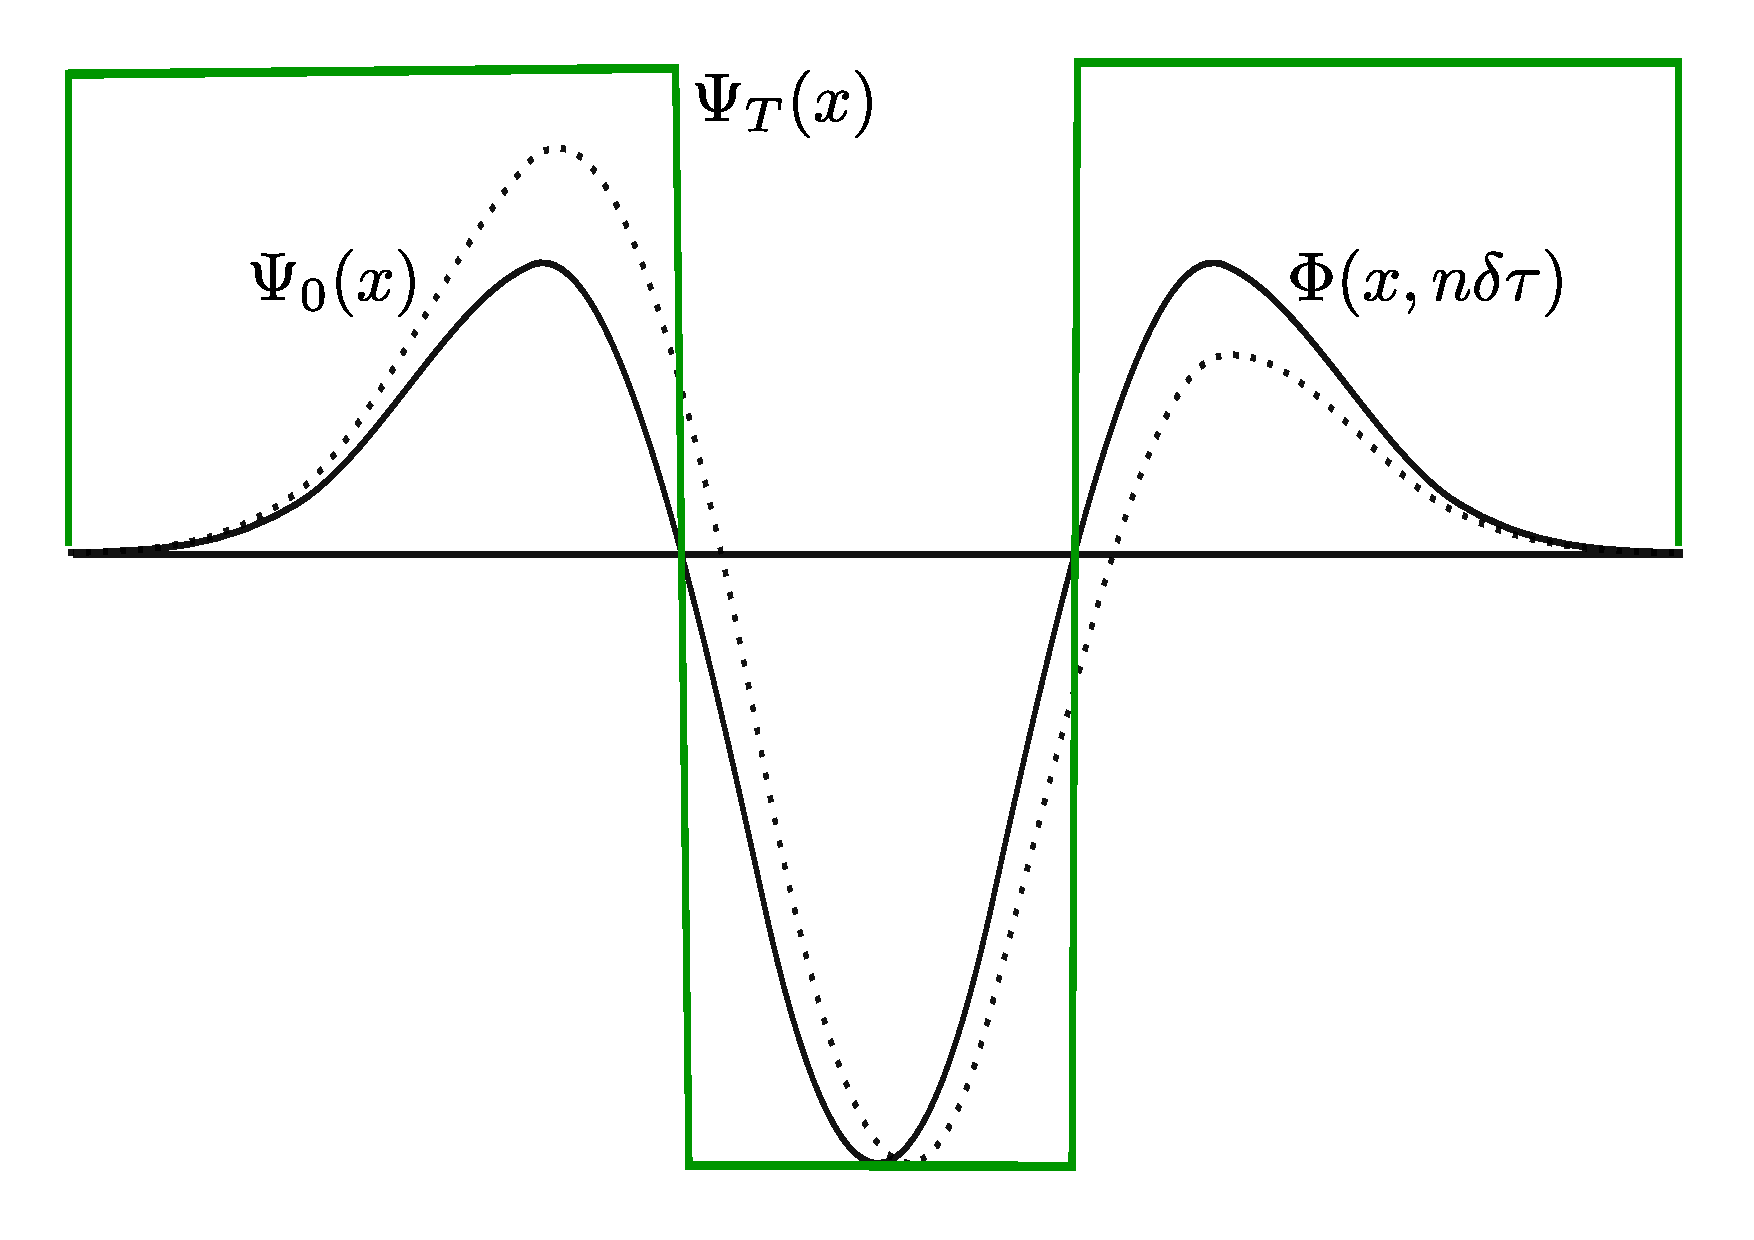
\includegraphics[scale=0.3]{../Graphics/fixxednode.pdf}
  \caption{A one-dimensional illustration of the fixed node approximation. The dotted line represents the exact ground state $\Psi_0(x)$. The distribution of walkers after $n$ Monte-Carlo cycles is represented by $\Phi(x, n\delta\tau)$. The trial wave function $\Psi_T(x)$ shares nodes with $\Phi(x, n\delta\tau)$, making it impossible for $\Phi(x, n\delta\tau)$ to match $\Psi_0(x)$.}
  \label{fig:fixxednode}
 \end{center}
\end{figure}


\section{Estimating One-body Densities}
\label{sec:OBD}

The one-body density is defined as

\begin{equation}
 \rho(  \mathbf{r}_1) = \iint\limits_{  \mathbf{r}_2   \mathbf{r}_3}...\int\limits_{  \mathbf{r}_N} \left|\Phi(  \mathbf{r}_1   \mathbf{r}_2 ...   \mathbf{r}_N)\right|^2\mathrm{d}  \mathbf{r}_2...\mathrm{d}  \mathbf{r}_N.
\end{equation}

Unlike the distribution $|\Phi(\mathbf{r})|^2$, which describes the distribution of any of the particles in the system, the one-body density $\rho(\mathbf{r}_1)$ describes the simultaneous distribution of every particle in the system, that is, $\rho(\mathbf{r}_1)\mathrm{d}\mathbf{r}_1$ represents the probability of finding \textit{any} of the system's $N$ particles within the volume element $\mathrm{d}\mathbf{r}_1$. Due to the indistinguishable nature of the particles, the fact that the first coordinate is chosen is purely conventional; any of the $N$ coordinates contain information about all the particles. For the same reason, the one-body density should be normalized to the number of particles, and not to unity.   

In a Monte-Carlo simulation, estimating the one-body density is done by collecting snapshots of the walkers' positions. These snapshots serve as samples to a histogram where each set of Cartesian coordinates give rise to one histogram-count.

\subsection{Estimating the Exact Ground State Density}

It was mentioned in the section on VMC that the final state of convergence was to have to walkers span the trial wave function. This implies that the one-body density of the trial wave function, called the \textit{variational density}, can be calculated using positional data generated from VMC.

The challenge lies in estimating the one-body density of the exact wave function given a set of DMC data. As described in Section \ref{sec:anisFokker}, the distribution of walkers span the \textit{mixed density} $f(\mathbf{r}, \tau) = \Ptau\PT$, which does not correspond to the ground state distribution unless the trial wave function is indeed the exact ground state. Hence a histogram of the DMC data does not suffice when it comes to presenting the exact wave function.

This implies the need of a method for transforming the one-body density of $f(\mathbf{r}, \tau)$ into the \textit{pure density} $|\Ptau|^2$. To achieve this, the following relation is needed \cite{abInitioMC}

\begin{align}
 \langle A \rangle_0 = \frac{\bra{\Phi_0}\OP{A}\ket{\Phi_0}}{\braket{\Phi_0}{\Phi_0}} &\simeq  2\frac{\bra{\Phi_0}\OP{A}\ket{\Psi_T}}{\braket{\Phi_0}{\Psi_T}} -  \frac{\bra{\Psi_T}\OP{A}\ket{\Psi_T}}{\braket{\Psi_T}{\Psi_T}} + \mathcal{O}(\Delta^2)\notag\\
  &= 2\langle A \rangle_\mathrm{DMC} - \langle A \rangle_\mathrm{VMC}  + \mathcal{O}(\Delta^2), \label{eq:PureEstimRelat}
\end{align}

where $\Delta \equiv \PT - \Ptau$. 

Expressed in terms of \textit{density operators}, the expectation values for the different methods are \cite{leinaas}

\newcommand{\tr}{\mathrm{tr}}

\begin{align*}
 \langle A \rangle_0 &= \tr(\OP{\rho}_0\OP{A}) \\
 \langle A \rangle_\mathrm{VMC} &= \tr(\OP{\rho}_\mathrm{VMC}\OP{A}) \\
 \langle A \rangle_\mathrm{DMC} &= \tr(\OP{\rho}_\mathrm{DMC}\OP{A}) 
 \end{align*}

where $\tr$ denotes the \textit{trace}, i.e. the sum of all eigenvalues. Inserting these equations into Eq.~(\ref{eq:PureEstimRelat}) yield

\begin{align}
 \tr(\OP{\rho}_0\OP{A}) &\simeq 2\tr(\OP{\rho}_\mathrm{DMC}\OP{A}) -  \tr(\OP{\rho}_\mathrm{VMC}\OP{A}) + \mathcal{O}(\Delta^2) \notag\\
  &\simeq \tr\left(\left(2\OP{\rho}_\mathrm{DMC} - \OP{\rho}_\mathrm{VMC}\right)\OP{A}\right) + \mathcal{O}(\Delta^2),
\end{align}

which leads to the conclusion that the mixed density can be transformed in the following manner:

\begin{equation}
 \OP{\rho}_0 \simeq 2\OP{\rho}_\mathrm{DMC} - \OP{\rho}_\mathrm{VMC} .\label{eq:densityTransform}
\end{equation}

It is clear that if this relation holds for regular densities, it will hold for one-body densities as well. In other words, the resulting densities from DMC can be combined with the corresponding one from VMC to produce the pure density.

\subsection{Radial Densities}

Integrating out every degree of freedom except one radial coordinate from the density results in the radial one-body density times the radius (squared for three dimensions). In other words

\begin{align}
 I_\mathrm{3D} &= \iint \rho (\mathbf{r}_1, \theta_1, \phi_1)r_1^2\sin\theta_1\mathrm{d}\theta_1\mathrm{d}\phi_1 \notag\\
   &\propto r_1^2\rho(\mathbf{r}_1), \label{eq:averagedRadialOBD_3D} \\
 I_\mathrm{2D} &= \int \rho (\mathbf{r}_1, \phi_1)r_1\mathrm{d}\phi_1 \notag\\
   &\propto r_1\rho(\mathbf{r}_1). \label{eq:averagedRadialOBD_2D}
\end{align}

In practice, these integrals are calculated by creating histograms $H(r)$ of all sampled radii. Transforming the histograms into radial one-body densities $\rho(r_1)$ are according to Eq.~(\ref{eq:averagedRadialOBD_3D}) and Eq.~(\ref{eq:averagedRadialOBD_2D}) done in the following manner

\begin{equation}
 \rho(\mathbf{r}_1) = \frac{H(\mathbf{r}_1)}{r_1^{(d-1)}},\label{eq:radial_OBD}
\end{equation}

where $d$ denotes the number of dimensions. An example presenting two radial one-body densities is given in Figure \ref{fig:OBD_ex}. Notice, however, that the radial density for certain systems such as atoms needs to be scaled with $r$ or $r^2$ in order to reveal the interesting shapes. 

\begin{figure}
 \begin{center}
  \subfigure{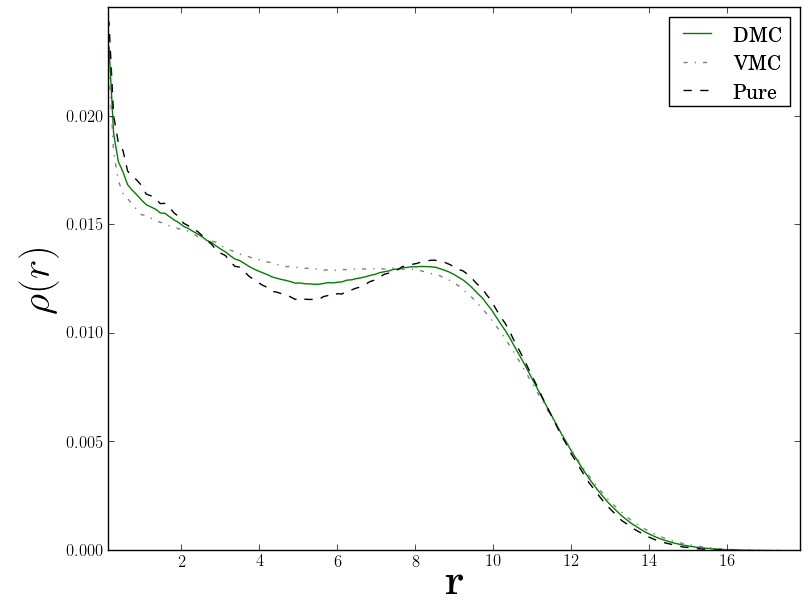
\includegraphics[scale=0.35]{../Graphics/OBD_rad_ex_12pw01.png}}
  \subfigure{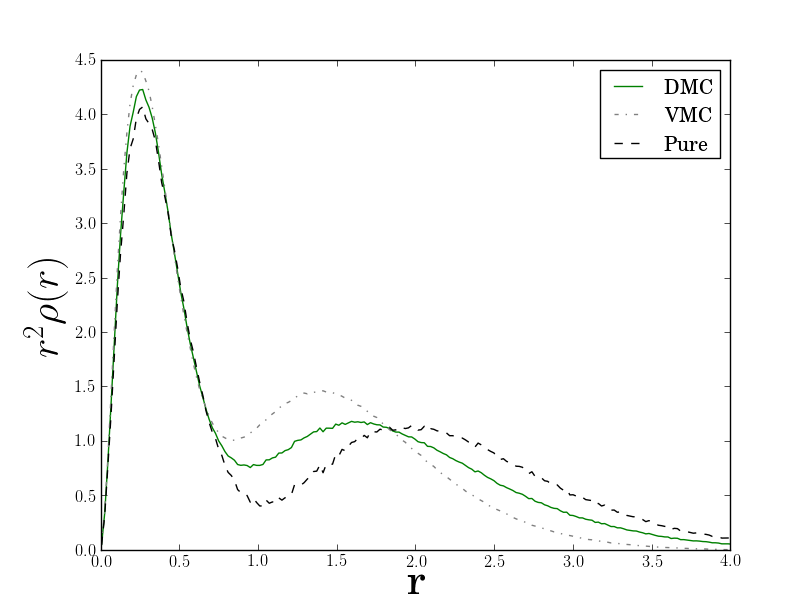
\includegraphics[scale=0.3816]{../Graphics/OBD/OBD_Atoms/2D/Beryllium.png}}
  \caption{Two examples of radial one-body densities for VMC, DMC, and the pure density from Eq.~(\ref{eq:densityTransform}). On the left: A 12-particle two-dimensional quantum dot with frequency $\omega=0.1$. The density diverges close to zero due to a ``$\frac{0}{0}$'' expression (see Eq.~(\ref{eq:radial_OBD})). On the right: Unscaled radial density for the beryllium atom, i.e.~$r_1^2\rho(\mathbf{r}_1)$. The densities will be discussed in the result section.}
  \label{fig:OBD_ex}
 \end{center}
\end{figure}



\section{Estimating the Statistical Error}

As with any statistical result, the statistical errors needs to be supplied in order for it to be taken seriously. Systematic errors, that is, errors introduced due to limitations in the model, is discussed in each method's respective section, and will not be related to the statistical error. 

Statistical errors, that is, the  deviation from the true ensemble average due to the fact that the equality in Eq.~(\ref{eq:MeanVStrueExp}) can never be fulfilled, can be estimated using several methods, some of which are \textit{naive} in the sense that they assume the dataset to be completely \textit{uncorrelated}, i.e. the samples are independent of each other.

\subsection{The Variance and Standard Deviates}
\label{sec:varAndSTD}

Given a set of samplings, e.g. local energies, the variance is a measure of their spread from the true mean value

\begin{eqnarray}
\label{eq:variance}
\Var(E) &=& \Exp{(E-\Exp{E})^2} \nonumber\\
        &=& \Exp{E^2} - 2\underbrace{\Exp{E\Exp{E}}}_{\Exp{E}\Exp{E}} + \Exp{E}^2 \nonumber\\
        &=& \Exp{E^2} - \Exp{E}^2 \\
        &\simeq& \overline{E^2} - \overline{E}^2
\end{eqnarray}

In the case of having the exact wave function, i.e $\ket{\Psi_T} = \ket{\Psi_0}$, the variance becomes zero:

\begin{eqnarray*}
\label{eq:varianceZeroExact}
\Var(E)_\mathrm{Exact} &=& \bra{\Psi_0}\OP{H}^2\ket{\Psi_0} -  \bra{\Psi_0}\OP{H}\ket{\Psi_0}^2 \\
		        &=& E_0^2 - (E_0)^2 \\
		        &=& 0
\end{eqnarray*}

The variance is in other words an excellent measure of how good of a fit different trial wave functions are to the system. A common misconception is that the numerical value of the variance can be used to compare properties of \textit{different} systems. For instance, if system $A$ has variance equal to half of system $B$'s, one could easily conclude that system $A$ has the best fitting trial wave function. However, this is not true. The variance has unit energy squared (in the case of local energies), and will thus scale with the magnitude of the energy. One can only safely use the variance as a direct measure locally in each specific system, e.g. Beryllium simulations.

Another misconception is that the variance is a direct numerical measure of the error. This can in no way be true given that the units mismatch. The \textit{standard deviation}, $\sigma$, is the square root of the variance,

\begin{equation}
\label{eq:stdNaive}
 \sigma^2(x) = \Var(x),
\end{equation}


and has hence a unit equal to that of the measured value. It is therefore related to the \textit{spread} in the sampled value; zero deviation implies perfect samples, while increasing deviation means increasing spread and statistical uncertainty. The standard deviation is in other words a useful quantity when it comes to calculating the error, i.e. the expected deviation from the exact mean $\Exp{E}$.

\subsection{The Covariance and correlated samples}

It was briefly mentioned in the introduction that certain error estimation techniques was too naive in case of correlated samples. Two samples, $x$, $y$, are said to be correlated if their \textit{covariance}, $\Cov(x, y)$, is non-zero

\begin{eqnarray}
\label{eq:covariance}
 \Cov(x, y) &\equiv& \Exp{(x - \Exp{x})(y - \Exp{y})} \nonumber\\
            &=& \Exp{xy - x\Exp{y} - \Exp{x}y + \Exp{x}\Exp{y}} \nonumber\\
            &=& \Exp{xy} - \Exp{x\Exp{y}} \underbrace{-\Exp{y\Exp{x}} + \Exp{\Exp{x}\Exp{y}}}_{0} \nonumber\\
            &=& \Exp{xy} - \Exp{x}\Exp{y}.
\end{eqnarray}

Notice that $\Cov(x,x) = \Var(x)$. Using this definition, whether or not the samples are correlated boils down to whether or not $\Exp{xy} = \Exp{x}\Exp{y}$. 

The consequence of ignoring the correlations is a resulting error estimate which is generally less than the true error; correlated samplings are more clustered, i.e. less spread, due to previous samplings' influence on the value of the current sample\footnote{Samples in QMC is obviously correlated due to the nature of the Langevin equation (difference equation).}. Denoting the true standard deviation as $\sigma_c$, the above discussion can be distilled to

\begin{equation}
 \label{eq:trueVsNaiveSTD}
 \sigma_c(x) \ge \sigma(x),
\end{equation}

where $\sigma(x)$ is the deviation from Eq.~(\ref{eq:stdNaive}). 


\subsection{The Deviate from the Exact Mean}

There is an important difference between the deviate from the exact mean, and the deviate of a single sample from its combined mean, in other words:

\begin{equation}
 \sigma(\overline{x}) \ne \sigma(x).
\end{equation}

Imagine doing a number of simulations, each resulting in a unique $\overline{x}$, the quantity of interest is not the deviation within a single simulation, but the deviation between the results of all the simulations.

\begin{eqnarray}
 m &\equiv& \overline{x} = \frac{1}{n}\sum_{i=1}^n x_i \label{eq:meanx}\\
 \sigma^2(m) &=& \Exp{m^2} - \Exp{m}^2 \label{eq:sigma_m}
\end{eqnarray}

Combining the above equations yields

\begin{eqnarray}
\label{eq:realErrorCovariance1}
  \sigma^2(m) &=& \Exp{\frac{1}{n^2}\left[\sum_{i=1}^nx_i\right]^2} - \Exp{\frac{1}{n}\sum_{i=1}^n x_i}^2 \nonumber\\
              &=& \frac{1}{n^2}\left( \Exp{\sum_{i=1}^n x_i\sum_{j=1}^n x_j} - \Exp{\sum_{i=1}^n x_i}\Exp{\sum_{j=1}^n x_j}  \right) \nonumber\\
              &=& \frac{1}{n^2}\sum_{i,j=1}^n \Exp{x_ix_j} - \Exp{x_i}\Exp{x_j} \nonumber\\
              &=& \frac{1}{n^2}\sum_{i,j=1}^n \Cov(x_i, x_j)
\end{eqnarray}

This result is important; the true error is given in terms of the covariance, and is, as discussed previously, only equal to the sample variance if the samples are uncorrelated. Going back to the definition of covariance in Eq.~(\ref{eq:covariance}), it is apparent that in order to calculate the covariance as in Eq.~(\ref{eq:realErrorCovariance1}), the true mean $\Exp{x_i}$ needs to be known. Using $m=\overline{x}$ as a necessary approximation to the true mean yields   

\begin{eqnarray}
 \Cov(x_i, x_j) &\equiv& \Exp{(x_i - \Exp{x_i})(x_j - \Exp{x_j})} \nonumber\\
                &\simeq& \Exp{(x_i - m)(x_j - m)} \nonumber\\
                &\simeq& \frac{1}{n^2}\sum_{k,l=1}^n (x_k-m)(x_l-m) \\
                &\equiv& \frac{1}{n}\Cov(x)
\end{eqnarray}

Inserting this relation into Eq.~(\ref{eq:realErrorCovariance1}) yields

\cfbox{2.7cm-8pt}{
\begin{eqnarray}
\label{eq:realErrorCovariance2}
   \sigma^2(m) &=& \frac{1}{n^2}\sum_{i,j=1}^n \Cov(x_i, x_j) \nonumber\\
               &\simeq& \frac{1}{n^2}\sum_{i,j=1}^n \frac{1}{n}\Cov(x) \nonumber\\
               &=& \frac{1}{n^3}\Cov(x)\underbrace{\sum_{i,j=1}^n}_{n^2}  \nonumber\\
               &=& \frac{1}{n} \Cov(x), \\
               \nonumber
\end{eqnarray}
}

which serves as an estimate of the full error including correlations. 

Explicitly computing the covariance is rarely done in Monte-Carlo simulations; if the sample size is large, it is extremely expensive. A variety of alternative methods to counter the correlations are available, the simplest of which is to define a \textit{correlation length}\footnote{In literature, this parameter is often referred to as the \textit{auto-correlation time}.}, $\tau$, which defines an interval at which points from the sampling sets are used for actual averaging. In other words, only the points $x_0, x_{\tau}, ..., x_{n\tau}$ are used in the calculation of $\overline{x}$

\begin{equation}
 \overline{x} = \frac{1}{n}\sum_{k=0}^n x_{k\cdot\tau}
\end{equation}

This implies that $n\tau$ samples are needed in order to get the same magnitude of samples to the average as in Eq.~(\ref{eq:meanx}); the \textit{effective sample size} becomes $n_\mathrm{eff} = n_\mathrm{tot}/\tau$. In the cases where $\tau = 1$, the sample set is uncorrelated. For details regarding the derivations of $\tau$ based on the covariance, see Refs. \cite{flyvbjerg:461} and \cite{morten}.

\subsection{Blocking}

Introducing correlation lengths in the system solver is not an efficient option. Neither is calculating the covariance of billions of data points. However, the error is not a value vital to the simulation process, i.e. there is no need to know the error at any stage during the sampling. This means that the error estimation can be done post process (given that the sample set is stored).

An efficient algorithm for calculating the error of correlated data is \textit{blocking}. This method is described in high detail in ref. \cite{flyvbjerg:461}, however, details aside, the idea itself is quite intuitive: Given a data set of $N$ samples from a single Monte-Carlo simulation, imagine dividing the dataset into \textit{blocks} of $n$ samples, that is, blocks of size  $n_b=N/n$. The error $\sigma_n$ in each block will naturally increase as $n$ decrease, (see Eq.~(\ref{eq:realErrorCovariance2}))

\begin{equation}
 \sigma_n \propto \frac{1}{\sqrt{n}}
\end{equation}


However, treating each block as an individual simulation, $n_b$ averages $m_n$ can be used to calculate the total error from Eq.~(\ref{eq:sigma_m}), that is, estimate the covariance

\begin{eqnarray}
  \overline{m_n^r} &\equiv& \frac{1}{n_b}\sum_{k=1}^{n_b} m_k^r \\
\nonumber\\
  \sigma^2(m) &=& \Exp{m^2} - \Exp{m}^2 \nonumber\\
              &\simeq& \overline{m_n^2} - (\overline{m_n})^2 \label{eq:blockingError}
\end{eqnarray}

The approximation should hold for a range of different block sizes, however, just as there is no a priori way of telling the correlation length, there is no a priori way of telling how many blocks is needed. However, what is known, is that if the system is correlated, there should be a range of different block sizes which fulfills Eq.~(\ref{eq:blockingError}) to reasonable precision. 

The result of a blocking analysis is therefore a series of ($n$, $\sigma(m)$) pairs which can be plotted. The plot should in light of previous arguments result in a increasing curve which stabilizes over a certain span of block sizes (where Eq.~(\ref{eq:blockingError}) is fulfilled). This plateau will then serve as a reasonable approximation to the covariance, that is, the true average. See Figure \ref{FIG:BlockingExamples} for a demonstration of resulting blocking plots.

\begin{figure}
 \begin{center}
  \subfigure{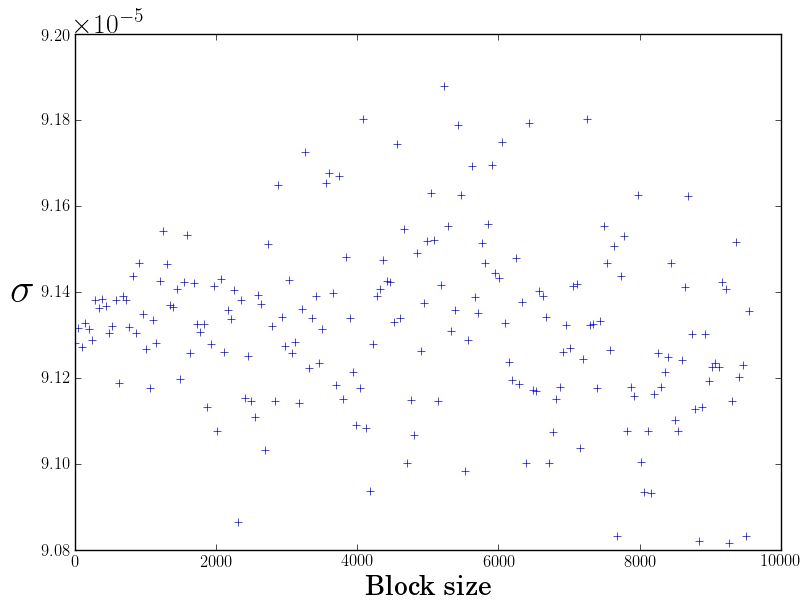
\includegraphics[scale=0.35]{../Graphics/BlockingExampleUncorr.png}}
  \subfigure{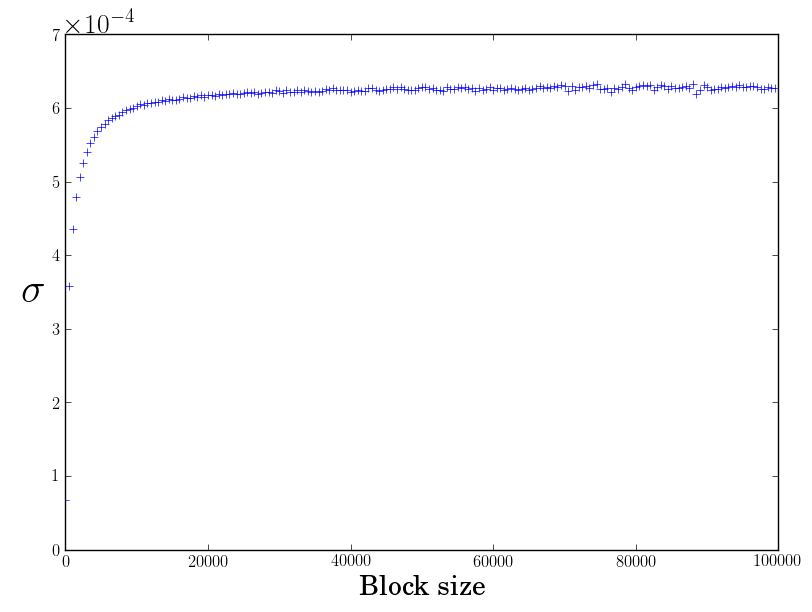
\includegraphics[scale=0.35]{../Graphics/BlockingExampleCorr.png}} 
  \caption{Left hand side: Blocking result of (approximately) uncorrelated data generated from a uniform Monte-Carlo integration of $\int _1^2 2x\mathrm{d}x$ resulting in $3.00003$ (exact is $3.0$). This is in excellent agreement with the magnitude of the error $\sim 9\cdot 10^{-5}$. There is no sign of a plateau, which implies fairly uncorrelated data (the span of the spread is small and apparently random). Right hand side: Blocking result of a DMC simulation of a 6-particle $\omega=0.1$ quantum dot. The plateau is strongly present, implying correlated data. The resulting total error is  $\sim 4.5\cdot 10^{-5}$.}
  \label{FIG:BlockingExamples}
 \end{center}
\end{figure}


\subsection{Variance Estimators}

The standard intuitive variance estimator

\begin{equation}
\label{eq:varBias}
 \sigma^2(x) \simeq \frac{1}{n}\sum_{i=1}^n (x_i - \overline{x})^2 = \left(\frac{1}{n}\sum_{i=1}^n x_i^2\right) - \overline{x}^2,
\end{equation}

is just an example of a variance estimator. A more precise estimator is 

\begin{equation}
\label{eq:varUnbias}
 \sigma^2(x) \simeq \frac{1}{n-1}\sum_{i=1}^n (x_i - \overline{x})^2 = \left(\frac{1}{n-1}\sum_{i=1}^n x_i^2\right) - \frac{n}{n-1}\overline{x}^2,
\end{equation}

which is only noticeably different from Eq.~(\ref{eq:varBias}) when the sample size gets small, as it does in blocking analysis. It is therefore standard to use Eq.~(\ref{eq:varUnbias}) for blocking errors.



\chapter{Generalization and Optimization}
\label{ch:optAndGen}

There is a big difference in strategy between writing code for a specific problem, and creating a general solver. A general Quantum Monte-Carlo (QMC) solver involves several layers of complexity, such as support for different potentials, single particle bases, sampling models, etc., which may easily lead to a combinatoric disaster if the planning is not done right. 

This chapter begins by introducing a list of underlying assumptions regarding the modelled systems. Whether or not a system can be solved is then a question of whether the listed assumptions are valid for the system or not. The next part will cover generalization, that is, the flexibility of the code and the strategies used to obtain this flexibility. The result of a generalized code is that different systems and algorithms can be implemented by making simple changes to the code. Finally, optimizations will be covered. Optimizations are crucial in order to maintain efficiency for a high number of particles. 

\section{Underlying Assumptions and Goals}
\label{sec:AssGoal}

In large computational projects it is custom to plan every single part of the program before the actual process of coding begins. Coding massive frameworks without planning almost exclusively result in unforeseen consequences, rendering the code difficult to expand, disorganized, and inefficient. The code used in this thesis has been completely restructured four times. This section will cover the assumptions regarding the modelled systems and the goals regarding generalization and optimization made in the planning stages preliminary to the coding process.

\subsection{Assumptions}
\label{sec:ass}

The code structure was designed based on the following assumptions

\cfbox{3cm-3pt}{
\begin{enumerate}[label=\textbf{(\roman{*})}, ref=(\roman{*}), align=left]
 \item The particles of the simulated systems are either all fermions or all bosons. \label{it::ass::pureFermBos}
 \item The Hamiltonian is spin - and time independent.\label{it::ass::2level}
 \item The trial wave function of a fermionic system is a single determinant. \label{it::ass::fermiSingleDet}
 \item A bosonic system is modelled by all particles being in the same assumed single particle ground state. \label{it::ass::bosCondensate}
 \vspace{0.3cm}
\end{enumerate}
}

As discussed in Section \ref{sec:trialWF}, the second assumption implies that the Slater determinant can be split into parts corresponding to different spin eigenvalues. The time-independence is a requirement on the QMC solver explained in Section \ref{sec:statingDiff}. The assumptions listed are considered true for any system which is implemented in the code, and will thus be applied in all of the following sections. 

\subsection{Generalization Goals}
\label{sec:genGoals}

The implementation should be general for:

\cfbox{3.17cm-1pt}{
\begin{enumerate}[label=\textbf{(\roman{*})}, ref=(\roman{*}), align=left]
 \item Fermions and Bosons. \label{it::gen::FermiAndBoson}
 \item Anisotropic- and isotropic diffusion, i.e.~Brute Force - or Importance sampling. \label{it::gen::BF_IS}
 \item Different gradient descent algorithms. 
 \item Any Jastrow factor.
 \item Any error estimation algorithm.
 \item Any single particle basis, including expanded single particle bases. \label{it::gen::SP_basis}
 \item Any combination of any potentials. \label{it::gen::pot}
 \vspace{0.2cm}
\end{enumerate}
}
 
In addition, the following constraint is set on solvers:

\cfbox{3.42cm-1pt}{
\begin{enumerate}[label=\textbf{(\roman{*})}, ref=(\roman{*}), align=left]
\setcounter{enumi}{7}
 \item Full numerical support for all values involving derivatives.\label{it::gen::numSupp}
 \vspace{0.2cm}
\end{enumerate}
}

The challenge is, despite the vast array of combinations, to preserve simplicity and structure as layers of complexity are added. Achieving generalization by the use of conditional if tests inside the solvers is considered inefficient, and should only be used if no other solution is apparent or exists.

\subsection{Optimization Goals}
\label{sec:optGoals}

Modern computers have a vast amount of physical memory available, which makes runtime optimizations favored over memory optimizations. The following list may appear short, but every step brings immense amounts of complexity to the implementation

\cfbox{3.6cm}{
\begin{enumerate}[label=\textbf{(\roman{*})}, ref=(\roman{*}), align=left]
 \item Identical values should never be re-calculated. \label{it::opt::reCalc}
 \item Generalization should not be achieved through conditional if tests in repeated function calls, but rather through polymorphism (see Section \ref{sec:typeCastPoly}). \label{it::opt::noIF}
 \item Linear scaling of runtime vs. the number of processors (CPUs) for large simulations. \label{it::opt::parScale}
 \vspace{0.2cm}
\end{enumerate}
}

Goal (\ref{it::opt::noIF}) has been the ground pillar of the code design. 

\clearpage
\section{Specifics Regarding Generalization}
\label{sec:specGen}

This section will introduce how object orientation is used to achieve the goals regarding generalization of the code. Several examples are discussed, however, for more details regarding the implementation of methods, see the code in Ref. \cite{libBorealisCode}.

\subsection{Generalization Goals \ref{it::gen::FermiAndBoson}-\ref{it::gen::pot}}

As discussed in Section \ref{sec:manyBodyWFs}, the mathematical difference between fermions and bosons (of importance to QMC) is how the many-body wave functions are constructed from the single-particle basis. In the case of fermions, the expression is given in terms of a Slater determinant which, due to the fact that the Hamiltonian is spin-independent, can be split into two parts corresponding to spin up and spin down. On the other hand, for bosons, it is simply the product of all states due to the fact that they are all assumed to occupy the same orbital. This is demonstrated in the following code example, where the wave functions of fermionic and bosonic systems are evaluated:

\vspace{0.2cm}
\begin{lstlisting}[caption=The implementation of the evaluation of fermionic and bosonic wave functions. Line 5: The fermion class accesses the walker's single particle state matrix and returns the determinant of the first half (spin up) times the determinant of the second half (spin down). Line 14-16: The boson class simply calculates the product of all the single particle states.]
double Fermions::get_spatial_wf(const Walker* walker) {
    using namespace arma;
    
    //Spin up times Spin down (determinants)
    return det(walker->phi(span(0, n2 - 1), span())) * det(walker->phi(span(n2, n_p - 1), span()));
}

double Bosons::get_spatial_wf(const Walker* walker) {
 
    double wf = 1;
 
    //Using the phi matrix as a vector in the case of bosons.
    //Assuming all particles to occupy the same single particle state (neglecting permutations).
    for (int i = 0; i < n_p; i++){
      wf *= walker->phi(i);
    }
    
    return wf;
}
\end{lstlisting}

Overloaded pure virtual methods for fermions and bosons exist for all of the methods which involves evaluating the many body wave function, for example the spatial ratio and the sum of Laplacians. When the \verb+QMC+ solver asks the \verb+System*+ object for a spatial ratio, depending on whether fermions or bosons are loaded run-time, the fermion or boson spatial ratio is evaluated. 

It is apparent that this way of implementing the system class takes care of optimization goal \ref{it::opt::noIF} in Section \ref{sec:optGoals} regarding no use of conditional if tests to determine the nature of the system. 

A similar polymorphic splitting is introduced in the following classes:

\begin{listliketab}
\storestyleof{itemize}
 \begin{tabular}{l l}
 \textbullet \,\verb+Orbitals+       & The hydrogen-like or the harmonic oscillator orbitals. \\
 \textbullet \,\verb+BasisFunctions+ & Stand-alone single particle wave functions initialized by \verb+Orbitals+. \\
 \textbullet \,\verb+Sampling+       & Brute force - or importance sampling. \\
 \textbullet \,\verb+Diffusion+      & Isotropic or Fokker-Planck diffusion. Automatically selected by \verb+Sampling+. \\
 \textbullet \,\verb+ErrorEstimator+ & Simple or Blocking. \\
 \textbullet \,\verb+Jastrow+        & Padé Jastrow - or no Jastrow factor. \\
 \textbullet \,\verb+QMC+            & Variational - (VMC) or diffusion Monte-Carlo (DMC). \\
 \textbullet \,\verb+Minimizer+      & Adaptive stochastic gradient descent (ASGD). \\
 \end{tabular}
\end{listliketab}

Implementing, for example, a new Jastrow Factor is done by simply creating a new subclass of \verb+Jastrow+. The QMC solver does not need to change to adapt to the new implementation. For more details, see Section \ref{sec:OO}. The splitting done in \verb+QMC+ is done to avoid rewriting a lot of general QMC code, such as diffusing walkers.

A detailed description of the generalization of potentials, i.e.~generalization goal \ref{it::gen::pot}, is given in Section \ref{sec:typeCastPoly}.

\subsection{Generalization Goal \ref{it::gen::SP_basis} and Expanded bases}

An expanded single particle basis is implemented as a subclass of the \verb+Orbitals+ superclass. It wraps around an \verb+Orbitals+ implementation, e.g.~the harmonic oscillator orbitals, containing basis elements $\phi_\alpha(\mathbf{r}_j)$. In addition to these elements, the expanded basis class has a set of expansion coefficients $\mathbf{C}_{\gamma\alpha}$ from which the new basis elements are constructed

\begin{equation}
\label{eq:ExpBasisSP}
 \psi_\gamma^\mathrm{Exp.}(r_j) = \sum_{\alpha=0}^{B - 1} \mathbf{C}_{\gamma\alpha}\phi_\alpha(r_j), 
\end{equation}

where $B$ is the size of the expanded basis. The following code snippet presents the vital members of the expanded basis class: 

\vspace{0.5cm}
\begin{lstlisting}[language=C++, caption={The declaration of the expanded basis class. The vital members are the size of the basis, the expansion coefficients and another basis in which the new are expanded. A method for calculating the coefficients is present, but the actual implementation has not been a focus of this thesis.}]
class ExpandedBasis : public Orbitals {

...

protected:

    int basis_size;
    arma::mat coeffs;
    Orbitals* basis;
    
    void calculate_coefficients();

};

\end{lstlisting}


The implementation of Eq.~(\ref{eq:ExpBasisSP}) into the expanded basis class is achieved by overloading the original \verb+Orbitals::phi+ virtual member function as shown in the following example

\vspace{0.5cm}
\begin{lstlisting}[caption=The explicit implementation of the expanded basis single particle wave function. The wave function is evaluated by expanding a given basis in a set of expansion coefficients (see the previous code example).]
double ExpandedBasis::phi(const Walker* walker, int particle, int q_num) {

    double value = 0;
    
    //Dividing basis_size by half assuming a two-level system.
    for (int m = 0; m < basis_size/2; m++) {
        value += coeffs(q_num, m) * basis->phi(walker, particle, m);
    }

    return value;

}
\end{lstlisting}

Expanded bases has not been a focus for the thesis, thus explicit algorithms for calculating the coefficients will not be covered. The reason the implementation has been presented, is to lay the foundation in case future Master students are to expand upon the code.

\subsection{Generalization Goal \ref{it::gen::numSupp}}

Support for evaluating derivatives numerically is important for two reasons; the first being debugging, the second being the cases where no closed-form expressions for the derivatives can be obtained or become too expensive to evaluate.

As an example, the orbital class implementation responsible for the gradient of the single particle states, \verb+Orbitals::del_phi+, is virtual. This implies that it can be overloaded to call the numerical derivative implementation \verb+Orbitals::num_diff+. The same goes for the Laplacian, the Jastrow factor derivatives, and the variational derivatives in the minimizer. An alternative to numerically evaluating the derivatives of the single particle wave functions would be to perform the derivative on the full many-body wave function, however, this would not fit naturally into the code design.

The implemented numerical derivatives are finite difference schemes with an error proportional to the square of the chosen step length.

\section{Optimizations due to a Single two-level Determinant}
\label{sec:optSingleSlater}

Assuming the trial wave function to consist of a single term unlocks several optimizations involving the Slater-determinant. Similar optimizations for bosons are considered trivial in comparison and will not be covered in detail. See the code in \cite{libBorealisCode} for details regarding bosons.

Writing the Slater determinant as the determinant of the \textit{Slater matrix} $\mathbf{S}$, the expression for the trial wave function in Eq.~(\ref{eq:singleDeterminantTWF}) becomes

\newcommand{\PTd}{|\mathbf{S}^\uparrow||\mathbf{S}^\downarrow |J}
\newcommand{\Du}{|\mathbf{S}^\uparrow|}
\newcommand{\Dd}{|\mathbf{S}^\downarrow|}
\newcommand{\Da }{|\mathbf{S}^{\alpha}|}
\newcommand{\Daa}{|\mathbf{S}^{\overline{\alpha}}|}
\newcommand{\PTda}{\Da\Daa J}

\begin{equation}
 \Psi_T = \PTd, \label{eq:phiTrialOptGen}
\end{equation}

where the splitting of the Slater determinant described in parts corresponding to spin up and spin down has been applied (see Eq.~(\ref{eq:splitSlater})). The Jastrow-factor, $J$, is described in section \ref{sec:ChoiceTrialWF}. Function arguments are skipped to clean up the expression. 

Several quantities involves evaluating the trial wave function, one of which are the quantum force from section \ref{sec:anisFokker} responsible for pushing the walkers in the direction of higher probabilities. Written in terms of Eq.~(\ref{eq:phiTrialOptGen}), the expression for the quantum force of particle $i$ becomes 

\begin{eqnarray}
 \mathbf{F}_i &=& 2\frac{\nabla_i\left(\PTd\right)}{\PTd} \nonumber\\
     &=& 2\left(\frac{\nabla_i\Du}{\Du} + \frac{\nabla_i\Dd}{\Dd} + \frac{\nabla_i J}{J}\right). \nonumber \\
\end{eqnarray}

The important part to realize now, is that particle $i$ \textit{either} has spin up or spin down. This implies that one of the derivatives in the last expression is zero due to the fact that the spins are opposite. Denoting the spin of particle $i$ as $\alpha$ and the opposite spin as $\overline{\alpha}$, the expressions for the quantum force reads

\begin{align}
 \mathbf{F}_i &= 2\left(\frac{\nabla_i\Da}{\Da} + \frac{\nabla_i\Daa}{\Daa} + \frac{\nabla_i J}{J}\right), \\ \nonumber
\end{align}

where 

\begin{equation}
 \nabla_i\Daa = 0, \label{eq:differentSpinDie}
\end{equation}

due to the fact that there is no trace of particle $i$ in $\Daa$. The resulting expression involves evaluating the Slater matrix for a single spin configuration only

\begin{equation}
 \mathbf{F}_i = 2\left(\frac{\nabla_i\Da}{\Da} + \frac{\nabla_i J}{J}\right). \nonumber
\end{equation}

The expression for the local energy from Section \ref{sec:calcExpVals} can be simplified in a similar manner. Starting from the original expression

\begin{equation}
 E_L = -\frac{1}{2}\sum_i \frac{1}{\Psi_T}\nabla^2_i \Psi_T + \sum_iV_i, \label{eq:localEsum}
\end{equation}

the Laplacian can be expanded in the same way as was done for the quantum force

 \begin{eqnarray}
  \frac{1}{\Psi_T}\nabla^2_i\Psi_T &=&  \frac{1}{\PTda}\nabla^2_i \PTda \nonumber\\
  &=& \frac{\nabla^2_i \Da}{\Da} + \frac{\nabla^2_i \Daa}{\Daa} + \frac{\nabla^2_i J}{J} \nonumber\\
  && +\,\, 2\frac{\left(\nabla_i\Da\right)\left(\nabla_i\Daa\right)}{\Da\Daa} + 2 \frac{\left(\nabla_i\Da\right)\left(\nabla_i J\right)}{\Da J} + 2 \frac{\left(\nabla_i\Daa\right)\left(\nabla_i J\right)}{\Daa J} \nonumber\\
  &=& \frac{\nabla^2_i \Da}{\Da} + \frac{\nabla^2_i J}{J} + 2\frac{\nabla_i\Da}{\Da} \frac{\nabla_i J}{J},
\end{eqnarray}

where half of the terms vanish due to Eq.~(\ref{eq:differentSpinDie}).

The last expression involving the Slater matrix (which can be simplified) is the spatial ratio, $R_\psi$, used in the Metropolis algorithm (see Section \ref{sec:MetroMain}). The expression reads

\begin{eqnarray}
 R_\psi &=& \frac{\Psi_T^\mathrm{new}}{\Psi_T^\mathrm{old}} \nonumber\\
 &=& \frac{\Du^\mathrm{new} \Dd^\mathrm{new} J^\mathrm{new}}{\Du^\mathrm{old} \Dd^\mathrm{old} J^\mathrm{old}}, \label{eq:R_psi_allspins}\\
\end{eqnarray}

where the old and new superscript denotes the wave function prior to and after moving one particle respectively. Let again $i$ be the currently moved particle with spin $\alpha$. As discussed previously, the part of the trial wave function representing the opposite spin of $\alpha$, $\Daa$, is independent of particle $i$. This implies that moving particle $i$ does not change the value of $\Daa$, that is

\begin{equation}
 \Daa^\mathrm{new} = \Daa^\mathrm{old}.
\end{equation}

Inserting this into Eq.~(\ref{eq:R_psi_allspins}) in addition to the spin parameters $\alpha$ and $\overline{\alpha}$ gives

\begin{equation}
 R_\psi = \frac{\Daa^\mathrm{new}}{\Daa^\mathrm{old}} = \underbrace{\frac{\Daa^\mathrm{new}}{\Daa^\mathrm{old}}}_{1}\frac{\Da^\mathrm{new}}{\Da^\mathrm{old}}\frac{J^\mathrm{new}}{J^\mathrm{old}} = \frac{\Da^\mathrm{new}}{\Da^\mathrm{old}}\frac{J^\mathrm{new}}{J^\mathrm{old}}. \label{eq:RpsiOpt}
\end{equation}

From the expressions deduced in this section it is clear that the dimensionality of the calculations is halved by splitting the Slater determinant into two parts. Calculating the determinant of a $N\times N$ matrix is $\mathcal{O}(N^2)$ floating point operations (flops), which implies a speedup of four in estimating the determinants alone. 

\section{Optimizations due to Single-particle Moves}

Moving a single particle at the time implies that only a single row in the Slater-determinant from Eq.~(\ref{eq:SlaterDeterminantExplicit}) will be changed between the calculations. Changes to a single row implies that many \textit{co-factors} remain unchanged. Since all of the expressions deduced in the previous section contains ratios of the spatial wave functions, expressing these determinants in terms of their co-factors should reveal a cancellation of terms. 

Expressing the cancellation mathematically presents the possibility to optimize the calculations by implementing only the parts which does not cancel. 

In the previous section it became apparent that only the determinant whose spin level matches that of the moved particle needs to be calculated explicitly. In the following sections, the spin indication on the Slater matrix $\Da$ will be skipped in order to clean up the equations.

\subsection{Optimizing the Slater ratios}
\label{sec:optSlaterRat}

\newcommand{\Sinv}{\mathbf{S}^{-1}}

The inverse of the Slater-matrix introduced in the previous section, is given in terms of its \textit{adjugate} by the following relation \cite{linAlg}

\begin{equation*}
 \Sinv = \frac{1}{|\mathbf{S}|}\mathrm{adj} \mathbf{S}.
\end{equation*}

The adjugate of a matrix is the transpose of the cofactor matrix $\mathbf{C}$. The expression in terms of matrix element equations reads

\begin{eqnarray}
 \Sinv &=& \frac{\mathbf{C}^T}{|\mathbf{S}|}, \\
 \Sinv_{ij} &=& \frac{\mathbf{C}_{ji}}{|\mathbf{S}|}\label{eq:invExpCofac}, \\
 \mathbf{S}_{ji} &=& \phi_i(\mathbf{r}_j). \label{eq:slaterMatPhi}
\end{eqnarray}

Moreover, the determinant can be expressed as a \textit{cofactor expansion} around row $j$ (Kramer's rule) \cite{linAlg}

\begin{equation}
\label{eq:cofacExp}
 |\mathbf{S}| = \sum_i \mathbf{S}_{ji} \mathbf{C}_{ji}.
\end{equation}

The spatial part of the $R_\psi$ ratio is obtained by inserting Eq.~(\ref{eq:cofacExp}) into Eq.~(\ref{eq:RpsiOpt})

\begin{equation}
\label{eq:RpsiCofac}
 R_S = \frac{\sum_i \mathbf{S}_{ji}^\mathrm{new}\mathbf{C}_{ji}^\mathrm{new}}{\sum_i \mathbf{S}_{ji}^\mathrm{old}\mathbf{C}_{ji}^\mathrm{old}}.
\end{equation}

Let $j$ represent the moved particle. The $j$'th column of the cofactor matrix is unchanged when the particle moves (column $j$ depends on every column but its own). In other words

\begin{equation}
 \mathbf{C}_{ji}^\mathrm{new} = \mathbf{C}_{ji}^\mathrm{old} = (\mathbf{S}^\mathrm{old}_{ij})^{-1}|\mathbf{S}^\mathrm{old}|,
\end{equation}

where the inverse relation of Eq.~(\ref{eq:invExpCofac}) has been used. Inserting this into Eq.~(\ref{eq:RpsiCofac}) yields

\begin{eqnarray}
  R_S &=& \frac{|\mathbf{S}^\mathrm{old}|}{|\mathbf{S}^\mathrm{old}|}\frac{\sum_i \mathbf{S}_{ji}^\mathrm{new}(\mathbf{S}_{ij}^\mathrm{old})^{-1}}{\sum_i \mathbf{S}_{ji}^\mathrm{old}(\mathbf{S}_{ij}^\mathrm{old})^{-1}} \nonumber\\
         &=& \frac{\sum_i \mathbf{S}_{ji}^\mathrm{new}(\mathbf{S}_{ij}^\mathrm{old})^{-1}}{\mathbf{I}_{jj}}. \nonumber
\end{eqnarray}

The diagonal element of the identity matrix is by definition unity. Inserting this fact combined with the relation from Eq.~(\ref{eq:slaterMatPhi}), an optimized expression for the ratio is obtained:

\cfbox{4cm-4pt}{
\begin{equation}
\label{eq:spatialRatioDet}
 R_S = \sum_i \phi_i(\mathbf{r}_j^\mathrm{new})(\mathbf{S}_{ij}^\mathrm{old})^{-1},
\end{equation}
}

where $j$ is the currently moved particle. The sum over $i$ spans the Slater matrix whose spin value matches that of particle $j$, i.e either $\mathbf{S}^\alpha$ or $\mathbf{S}^{\overline{\alpha}}$ (see the previous section).

Similar reductions can be applied to all the Slater ratio expressions from the previous section \cite{abInitioMC, morten}:

\cfbox{4cm}{
\begin{eqnarray}
 \frac{\nabla_i|\mathbf{S}|}{|\mathbf{S}|} &=& \sum_{k} \nabla_i\phi_k(r_i^\mathrm{new})(\mathbf{S}_{ki}^\mathrm{new})^{-1}, \\
  \frac{\nabla_i^2|\mathbf{S}|}{|\mathbf{S}|} &=& \sum_{k} \nabla_i^2\phi_k(r_i^\mathrm{new})(\mathbf{S}_{ki}^\mathrm{new})^{-1},
\end{eqnarray}
}

where the sum $k$ spans the Slater matrix whose spin values match that of the moved particle.

Closed form expressions for the derivatives and Laplacians of the single particle wave functions can be implemented in order to avoid expensive numerical calculations. See Appendices \ref{appendix:SymPyHO}, \ref{appendix:SymPyHO3D} and \ref{appendix:SymPyHydro} for a tabulation of closed form expressions used in this Thesis. Appendix \ref{appendix:sympy} presents an efficient strategy for obtaining these expressions.

\subsection{Optimizing the Inverse}
\label{sec:optInv}

One might question the efficiency of calculating inverse matrices compared to brute force estimation of the determinants. The efficiency of the inverse becomes apparent, as with the ratio in Eq.~(\ref{eq:spatialRatioDet}), by co-factor expanding the expression; an updating algorithm which dramatically decreases the cost of calculating the inverse of the new Slater matrix can be implemented.

Let $i$ denote the currently moved particle. The new inverse is given in terms of the previous by the following expression \cite{abInitioMC, morten}

\cfbox{4.5cm-5pt}{
\begin{eqnarray}
 \mathbf{\tilde I}_{ij} &=& \sum_l \mathbf{S}_{il}^\mathrm{new}(\mathbf{S}_{lj}^\mathrm{old})^{-1}, \\
 \ \label{eq:Itilde}\
 (\mathbf{S}_{kj}^\mathrm{new})^{-1} &=& (\mathbf{S}_{kj}^\mathrm{old})^{-1} - \frac{1}{R_S}(\mathbf{S}_{ji}^\mathrm{old})^{-1}\tilde I_{ij} \qquad\qquad j \ne i,\\
 (\mathbf{S}_{ki}^\mathrm{new})^{-1} &=& \frac{1}{R_S}(\mathbf{S}_{ki}^\mathrm{old})^{-1} \qquad\qquad\qquad\qquad\qquad\,\, \mathrm{else}. \\
 \ \nonumber
\end{eqnarray}
}

This reduces the cost of calculating the inverse by an order of magnitude down to $\mathcal{O}(N^2)$.

Further optimization can be achieved by calculating the $\mathbf{\tilde I}$ vector for particle $i$ prior to performing the loop over $k$ and $j$. Again, this loop should only update the inverse Slater matrix whose spin value correspond to that of the moved particle.

\subsection{Optimizing the Padé Jastrow factor Ratio}
\label{sec:optPagejastRat}

Such as was done with the Green's function ratio in Eq.~(\ref{eq:MetropolisHastings}), the ratio between two Jastrow factors are best expressed in terms of the logarithm

\begin{eqnarray}
 \log \frac{J^\mathrm{new}}{J^\mathrm{old}} &=& \sum_{k<j = 1}^N \left[\frac{a_{kj}r^\mathrm{new}_{kj}}{1 + \beta r^\mathrm{new}_{kj}} - \frac{a_{kj}r^\mathrm{old}_{kj}}{1 + \beta r^\mathrm{old}_{kj}}\right] \\
                      &\equiv& \sum_{k<j = 1}^N \left[g^\mathrm{new}_{kj} - g^\mathrm{old}_{kj}\right]. \label{eq:jastrowRatSTD}
\end{eqnarray}

The relative distances $r_{kj}$ behave much like the cofactors in Section \ref{sec:optSlaterRat}: Changing $r_i$ changes only $r_{ij}$, that is

\begin{equation}
 r^\mathrm{new}_{kj} = r^\mathrm{old}_{kj} \qquad k \ne i, 
\end{equation}

which inserted into Eq.~(\ref{eq:jastrowRatSTD}) yields

\begin{eqnarray}
  \log\frac{J^\mathrm{new}}{J^\mathrm{old}} &=& \sum_{k<j \ne i}  \underbrace{\left[g^\mathrm{old}_{kj} - g^\mathrm{old}_{kj}\right]}_{0} + \sum_{j = 1}^N \left[ g^\mathrm{new}_{ij} - g^\mathrm{old}_{ij}\right] \nonumber\\
                                            &=& \sum_{j = 1}^N a_{ij}\left(\frac{r^\mathrm{new}_{ij}}{1 + \beta r^\mathrm{new}_{ij}} - \frac{r^\mathrm{old}_{ij}}{1 + \beta r^\mathrm{old}_{ij}}\right).
\end{eqnarray}

Exponentiating both sides reveals the final optimized ratio 

\cfbox{4.6cm-2pt}{
\begin{equation}
 \frac{J^\mathrm{new}}{J^\mathrm{old}} = \exp \left[\sum_{j = 1}^N a_{ij}\left(\frac{r^\mathrm{new}_{ij}}{1 + \beta r^\mathrm{new}_{ij}} - \frac{r^\mathrm{old}_{ij}}{1 + \beta r^\mathrm{old}_{ij}}\right)\right].
\end{equation}
}


\section{Optimizing the Padé Jastrow Derivative Ratios}


The shape of the Padé Jastrow factor is general in the sense that it is independent of the system at hand. Calculating closed form expressions for the derivatives is then a process which can be done once and for all. 

Closed form expressions are not only very efficient compared to a numerical evaluation, but also exact to machine precision. These facts renders closed form expressions of high interest to any Monte-Carlo implementation. 

\subsection{The Gradient}

Using the notation of Eq.~(\ref{eq:jastrowRatSTD}), the $x$-component of the Padé Jastrow gradient ratio for particle $i$ is

\begin{equation}
 \frac{1}{J}\frac{\partial J}{\partial x_i} = \frac{1}{\prod_{k < l}\exp g_{kl}}\frac{\partial }{\partial x_i}\prod_{k < l}\exp g_{kl}.
\end{equation}

Using the product rule, the above product will be transformed into a sum, where only the terms which has $k$ or $l$ equal to $i$ survive the differentiation. In addition, the terms independent of $i$ will cancel the corresponding terms in the denominator. Performing this calculation yields

\begin{eqnarray}
  \frac{1}{J}\frac{\partial J}{\partial x_i} &=& \sum_{k \ne i} \frac{1}{\exp g_{ik}}\frac{\partial}{\partial x_i} \exp g_{ik} \nonumber\\
  &=& \sum_{k \ne i} \frac{1}{\exp g_{ik}}\frac{\partial g_{ik}}{\partial x_i} \exp g_{ik}\nonumber \\
  &=& \sum_{k \ne i} \frac{\partial g_{ik}}{\partial x_i} \nonumber \\
  &=& \sum_{k \ne i} \frac{\partial g_{ik}}{\partial r_{ik}}\frac{\partial r_{ik}}{\partial x_i},
\end{eqnarray}

where

\begin{eqnarray}
 \frac{\partial g_{ik}}{\partial r_{ik}} &=& \frac{\partial }{\partial r_{ik}} \left(\frac{a_{ik}r_{ik}}{1 + \beta r_{ik}}\right) \nonumber\\
  &=& \frac{a_{ik}}{1 + \beta r_{ik}} - \frac{a_{ik}r_{ik}}{(1 + \beta r_{ik})^2}\beta \nonumber \\
  &=& \frac{a_{ik}(1 + \beta r_{ik}) - a_{ik}\beta r_{ik}}{(1 + \beta r_{ik})^2}  \nonumber \\
  &=& \frac{a_{ik}}{(1 + \beta r_{ik})^2}, \label{eq:jastrowDgikDrik}
\end{eqnarray}

and

\begin{eqnarray}
 \frac{\partial r_{ik}}{\partial x_i} &=& \frac{\partial }{\partial x_i} \sqrt{(x_i - x_k)^2 + (y_i - y_k)^2 + (z_i - z_k)^2} \nonumber \\
  &=& \frac{1}{2} 2(x_i - x_k) / \sqrt{(x_i - x_k)^2 + (y_i - y_k)^2 + (z_i - z_k)^2} \nonumber \\
  &=& \frac{x_i - x_k}{r_{ik}}.
\end{eqnarray}

Combining these expressions yields

\begin{equation}
\label{eq:jastrowDerivX}
 \frac{1}{J}\frac{\partial J}{\partial x_i} = \sum_{k \ne i} \frac{a_{ik}}{r_{ik}}\frac{x_i - x_k}{(1 + \beta r_{ik})^2}.
\end{equation}

Changing the Cartesian variable in the differentiation changes only the numerator of Eq.~(\ref{eq:jastrowDerivX}). In other words, generalizing to the full gradient is done by substituting the Cartesian difference with the position vector difference. The expression for the gradient becomes

\cfbox{4.8cm}{
\begin{equation}
\label{eq:jastrowGradFull}
 \frac{\nabla_i J}{J} = \sum_{k \ne i = 1}^N \frac{a_{ik}}{r_{ik}}\frac{\mathbf{r}_i - \mathbf{r}_k}{(1 + \beta r_{ik})^2}.
\end{equation}
}


\subsection{The Laplacian}

The same strategy used to obtain the closed form expression for the gradient in the previous section can be applied to the Laplacian. The full calculation is done in ref. \cite{morten}. The expression becomes

\begin{equation}
\label{eq:jastrowLaplRaw}
 \frac{\nabla^2_i J}{J} = \left| \frac{\nabla_i J}{J}\right|^2 + \sum_{k \ne i = 1}^N \left(\frac{d-1}{r_{ik}}\frac{\partial g_{ik}}{\partial r_{ik}} + \frac{\partial^2 g_{ik}}{\partial r_{ik}^2}\right) 
\end{equation}

where $d$ is the number of dimensions arising due to the fact that the Laplacian, unlike the gradient, is a summation of contributions from all dimensions. A simple differentiation of Eq.~(\ref{eq:jastrowDgikDrik}) with respect to $r_{ik}$ yields

\begin{equation}
\label{eq:jastrowD2gikDrik2}
 \frac{\partial^2 g_{ik}}{\partial r_{ik}^2} = -\frac{2a_{ik}\beta}{(1 + \beta r_{ik})^3}
\end{equation}

Inserting Eq.~(\ref{eq:jastrowDgikDrik}) and Eq.~(\ref{eq:jastrowD2gikDrik2}) into Eq.~(\ref{eq:jastrowLaplRaw}) further reveals

\begin{eqnarray}
 \frac{\nabla^2_i J}{J} &=& \left| \frac{\nabla_i J}{J}\right|^2 + \sum_{k \ne i = 1}^N \left(\frac{d-1}{r_{ik}}\frac{a_{ik}}{(1 + \beta r_{ik})^2} - \frac{2a_{ik}\beta}{(1 + \beta r_{ik})^3}\right) \nonumber\\
  &=& \left| \frac{\nabla_i J}{J}\right|^2 + \sum_{k \ne i = 1}^N a_{ik}\frac{(d-1)(1 + \beta r_{ik}) - 2\beta r_{ik}}{r_{ik}(1 + \beta r_{ik})^3}, \nonumber
\end{eqnarray}

which when cleaned up results in

\begin{equation}
 \frac{\nabla^2_i J}{J} = \left| \frac{\nabla_i J}{J}\right|^2 + \sum_{k \ne i} a_{ik}\frac{(d-3)(\beta r_{ik} + 1) + 2}{r_{ik}(1 + \beta r_{ik})^3}.
\end{equation}

The local energy calculation needs the sum of the Laplacians for all particles (see Eq.~(\ref{eq:localEsum})). In other words, the quantity of interest becomes

\begin{equation}
 \sum_i \frac{\nabla^2_i J}{J} = \sum_i \left[\left|\frac{\nabla_i J}{J}\right|^2 + \sum_{k \ne i}^N a_{ik}\frac{(d-3)(\beta r_{ik} + 1) + 2}{r_{ik}(1 + \beta r_{ik})^3}\right].
\end{equation}

Due to the symmetry of $r_{ik}$, the second term count equal values twice. Further optimization can thus be achieved by calculation only terms where $k>i$, and multiply the sum by two. Bringing it all together yields

\cfbox{5cm}{
\begin{equation}
\label{eq:jastrowLaplFin}
 \sum_i \frac{\nabla^2_i J}{J} = \sum_i \left|\frac{\nabla_i J}{J}\right|^2 + 2\sum_{k > i} a_{ik}\frac{(d-3)(\beta r_{ik} + 1) + 2}{r_{ik}(1 + \beta r_{ik})^3}
\end{equation}
}


\section{Tabulating Recalculated Data}

The expressions introduced so far in this chapter contain terms which are identical. Explicitly calculating these terms every time they are countered in the code would waste a lot of CPU time in contrast to the optimal scenario where they are calculated only once.

Tabulating data is crucial in order for the code to remain efficient for an increased number of particles. 

\subsection{The relative distance matrix}
\label{sec:relDist}

In the discussions regarding the optimization of the Jastrow ratio in section \ref{sec:optPagejastRat}, it became clear that moving one particle only changed $N$ of the relative distances. Tabulating these distances in a matrix $\mathbf{r}_\mathrm{rel}$, which then can be updated when a particle is moved, will ensure that the relative distances are calculated once and for all. The matrix is set up in the following manner

\begin{equation}
\mathbf{r}_\mathrm{rel} = \mathbf{r}_\mathrm{rel}^T = \left( \begin{array}{ccccc}
0 & r_{12} & r_{13} & \cdots & r_{1N} \\
r_{21} & 0 & r_{23} & \cdots & r_{2N}  \\
 &  & \ddots & \ddots & \vdots \\
 & \cdots &  & 0 & r_{(N-1)N} \\
 &  &  &  & 0\end{array} \right),
\end{equation}

where the first equality expresses that the matrix is symmetric, that is, equal to it's own transpose. The following code presents the updating of the matrix when a particle is moved

\vspace{0.25cm}
\begin{lstlisting}[caption={The code used to update the relative distance matrix of a walker when a particle is moved. Pay extra attention to line 8 where the symmetry of the matrix is exploited to further decrease the number of calls to the relative distance function in line 9.}]
void Sampling::update_pos(const Walker* walker_pre, Walker* walker_post, int particle) const {

    ...

    //Updating the part of the r_rel matrix which is changed by moving the [particle]
    for (int j = 0; j < n_p; j++) {
        if (j != particle) {
            walker_post->r_rel(particle, j) = walker_post->r_rel(j, particle)
                    = walker_post->calc_r_rel(particle, j);
        }
    }
    
    ...

}
\end{lstlisting}


Functions such as \verb+Coulomb::get_potential_energy+ and all of the Jastrow functions can then simply access these matrix elements without having to perform any explicit calculations.

A similar updating algorithm has been implemented for the squared distance vector and the absolute value of the distance vector. 

\subsection{The Slater related matrices}
\label{sec:storeSlater}

Apart from the inverse, whose optimization was covered in Section \ref{sec:optInv}, calculating the single particle wave functions and its gradients are the most expensive operations in the QMC algorithm.

Storing these function values in matrices representing the Slater matrices $\mathbf{S}^\uparrow$ and $\mathbf{S}^\downarrow$ introduced in Section \ref{sec:optSingleSlater}, ensures that these values never gets recalculated. The following expression describes how the Slater matrix is represented in the code 

\begin{equation}
\label{eq:slaterConcat}
 \mathbf{S}  \equiv \mathrm{join}\left(\mathbf{S}^\uparrow,\,\,\mathbf{S}^\downarrow\right) = \left[ \begin{array}{cccc}
\phi_1(\mbf{r}_0)     & \phi_1(\mbf{r}_1)     & \cdots & \phi_1(\mbf{r}_N)       \\
\phi_2(\mbf{r}_0)     & \phi_2(\mbf{r}_1)     & \cdots & \phi_2(\mbf{r}_N)       \\
\vdots          & \vdots          &        & \vdots            \\
\phi_{N/2}(\mbf{r}_0) & \phi_{N/2}(\mbf{r}_1) & \cdots & \phi_{N/2}(\mbf{r}_N)   \end{array} \right],
\end{equation}

where $\mathrm{join}(\mathbf{A}, \mathbf{B})$ denotes joining the columns of the matrices $A$ and $B$, i.e. \textit{concatenate} the matrices\cite{linAlg}. Similarly for the gradient terms, the following matrix is responsible for storing the gradient of all the elements in Eq.~(\ref{eq:slaterConcat})

\begin{equation}
\label{eq:slaterDellConcat}
 \mathbf{dS} \equiv \left[ \begin{array}{cccc}
\nabla \phi_1(\mbf{r}_0)     & \nabla \phi_1(\mbf{r}_1)     & \cdots & \nabla \phi_1(\mbf{r}_N)       \\
\nabla \phi_2(\mbf{r}_0)     & \nabla \phi_2(\mbf{r}_1)     & \cdots & \nabla \phi_2(\mbf{r}_N)       \\
\vdots                 & \vdots                 &        & \vdots                   \\
\nabla \phi_{N/2}(\mbf{r}_0) & \nabla \phi_{N/2}(\mbf{r}_1) & \cdots & \nabla \phi_{N/2}(\mbf{r}_N)   \end{array} \right].
\end{equation}

The inverse Slater matrices are implemented this way as well:

\begin{equation}
 \Sinv \equiv \mathrm{join}\left((\mathbf{S}^\uparrow)^{-1}\,\,,(\mathbf{S}^\downarrow)^{-1}\right).
\end{equation}

In the code, these matrices are stored as \verb+walker.phi+, \verb+walker.del_phi+ and \verb+walker.inv+. When one particle is moved, only a single row in the two first matrices needs to be recalculated, and only half of the concatenated inverse needs to be updated.

This concatenation of matrices ensures that no conditional tests are needed in order to access the correct matrix for a given particle. 

\subsection{The Padé Jastrow gradient}
\label{sec:optJastGrad}

Just as for the Jastrow Laplacian, there are symmetries in the expression for the gradient in Eq.~(\ref{eq:jastrowGradFull}), which implies an optimized way of calculating it. However, unlike the Laplacian, the gradient is split into components, which makes the exploitation of symmetries a little less straight-forward. 

Defining

\begin{equation}
 \mathrm{d}\mbf{J}_{ik}  \equiv \frac{a_{ik}}{r_{ik}}\frac{\mathbf{r}_i -  \mathbf{r}_k}{(1 + \beta r_{ik})^2},
\end{equation}

it is apparent that 

\begin{equation}
 \mathrm{d}\mbf{J}_{ik} = -\mathrm{d}\mbf{J}_{ki}.
\end{equation}

Since the gradient can be written in terms of this quantity, that is,

\begin{equation}
 \frac{\nabla_i J}{J} = \sum_{k \ne i = 1}^N \mathrm{d}\mbf{J}_{ik},
\end{equation}

the code can be optimized by exploiting this antisymmetry. Consider the following matrix

\begin{equation}
\label{eq:jastrowDJ}
 \mathbf{\mathrm{d}J}\equiv \left( \begin{array}{ccccc}
0 & \mathrm{d}\mbf{J}_{12} & \mathrm{d}\mbf{J}_{13} & \cdots & \mathrm{d}\mbf{J}_{1N} \\
 -\mathrm{d}\mbf{J}_{12} & 0 & \mathrm{d}\mbf{J}_{23} & \cdots & \mathrm{d}\mbf{J}_{2N}  \\
 &  & \ddots & \ddots & \vdots \\
 & (-) &  & 0 & \mathrm{d}\mbf{J}_{(N-1)N} \\
 &  &  &  & 0\end{array} \right).
\end{equation}

In the same way that the relative distance matrix was equal to its transpose, the matrix above is equal to the negative of its transpose. In other words:

\begin{equation}
 \mathrm{d}\mathbf{J} = -\mathrm{d}\mathbf{J}^T.
\end{equation}

Additionally, just as for the relative distances, moving a single particle only changes one row and one column in the matrix. This implies that a similar updating algorithm as the one discussed in section \ref{sec:relDist} can be implemented. This is demonstrated in the following code snippet

\vspace{0.25cm}
\begin{lstlisting}[caption={The updating algorithm for the three dimensional matrix used in the Padé Jastrow gradient. Pay close attention to line 11, where the symmetry property is exploited by setting the transposed term equal to the negative of an already calculated term.}]
void Pade_Jastrow::get_dJ_matrix(Walker* walker, int moved_particle) const {
    
    int i = moved_particle;
    for (int j = 0; j < n_p; j++) {
	if (j == i) continue;
	
        b_ij = 1.0 + beta * walker->r_rel(i, j);
        factor = a(i, j) / (walker->r_rel(i, j) * b_ij * b_ij);
        for (int k = 0; k < dim; k++) {
            walker->dJ(i, j, k) = (walker->r(i, k) - walker->r(j, k)) * factor;
            walker->dJ(j, i, k) = -walker->dJ(i, j, k);
        }
    }
}
\end{lstlisting}


Calculating the new gradient is now only a matter of summing the rows of the matrix in Eq.~(\ref{eq:jastrowDJ}):

\begin{equation}
\frac{\nabla_i J^\mathrm{old}}{J^\mathrm{old}} = \sum_{k \ne i = 1}^N \mathrm{d}\mbf{J}^\mathrm{old}_{ik}.\label{eq:jastrowGraDJold}
\end{equation}

Further optimization can be achieved by realizing that the function which calculates the new gradient also has access to the gradient of the previous iteration

\begin{equation}
 \frac{\nabla_i J^\mathrm{new}}{J^\mathrm{new}} = \sum_{k \ne i = 1}^N \mathrm{d}\mbf{J}^\mathrm{new}_{ik}. \label{eq:jastrowGradDJnew}
\end{equation}

As mentioned previously, moving a particle, $p$, only a single row and column in $\mathrm{d} J$. For all other particles $i\ne p$, only a single term from the new matrix is required to update the old gradient

\begin{equation}
 \frac{\nabla_{i\ne p} J^\mathrm{new}}{J^\mathrm{new}} = \sum_{k = 1}^N \mathrm{d}\mbf{J}^\mathrm{new}_{ik} = \left[\sum_{k \ne p} \mathrm{d}\mbf{J}^\mathrm{old}_{ik}\right] + \mathrm{d}\mbf{J}^\mathrm{new}_{ip}.
\end{equation}

Adding and subtracting the term missing from the sum to make it equal to the old gradient from Eq.~(\ref{eq:jastrowGraDJold}) gives

\begin{eqnarray}
 \frac{\nabla_{i\ne p} J^\mathrm{new}}{J^\mathrm{new}} &=& \left[\sum_{k \ne p} \mathrm{d}\mbf{J}^\mathrm{old}_{ik} + \mathrm{d}\mbf{J}^\mathrm{old}_{ip}\right] - \mathrm{d}\mbf{J}^\mathrm{old}_{ip} + \mathrm{d}\mbf{J}^\mathrm{new}_{ip} \\
 &=& \frac{\nabla_i J^\mathrm{old}}{J^\mathrm{old}} - \mathrm{d}\mbf{J}^\mathrm{old}_{ip} + \mathrm{d}\mbf{J}^\mathrm{new}_{ip}, \label{eq:jastrowGradOptDJ}
\end{eqnarray}

effectively reducing the calculation to three flops. For the case where $i=p$, the entire sum must be calculated as in Eq.~(\ref{eq:jastrowGradDJnew}). This process is demonstrated in the following code

\vspace{0.25cm}
\begin{lstlisting}[caption={The implementation of the Padé Jastrow gradient using the matrix from Eq.~(\ref{eq:jastrowDJ}). Lines 18-25 describe the case for gradients not equal to the moved particle, i.e. Eq.~(\ref{eq:jastrowGradOptDJ}). Lines 5-18 describe the case for the gradient of the moved particle, where the full sum is calculated as Eq.~(\ref{eq:jastrowGradDJnew}).}]
void Pade_Jastrow::get_grad(const Walker* walker_pre, Walker* walker_post, int p) const {
    double sum;

    for (int i = 0; i < n_p; i++) {
        if (i == p) {
       
            //for i == p the entire sum needs to be calculated
            for (int k = 0; k < dim; k++) {

                sum = 0;
                for (int j = 0; j < n_p; j++) {
                    sum += walker_post->dJ(p, j, k);
                }

                walker_post->jast_grad(p, k) = sum;
            }
        
        } else {
       
            //for i != p only one term differ from the old and the new matrix
            for (int k = 0; k < dim; k++) {
                walker_post->jast_grad(i, k) = walker_pre->jast_grad(i, k)
                        + walker_post->dJ(i, p, k) - walker_pre->dJ(i, p, k);
            }
        }
    }
}
\end{lstlisting}

The dimensions of $\mathrm{d}\mathbf{J}$ are $N\times N\times d$, where $N$ is the number of particles and $d$ is the dimension. This implies that the optimizations in the Jastrow gradient discussed in this section scales very well with $N$. See Section \ref{sec:optRes} for a demonstration of the speedup in a $N=30$, $d=2$ case. 


\subsection{The single-particle Wave Functions}
\label{sec:optSPWFqnumIndie}

For systems of many particles, the function call \verb+Orbitals::phi(walker, i, qnum)+ needs to figure out which expression is related to which quantum number. The brute force implementation is to simply perform an if test on the quantum number, and use this to return the corresponding expression. This is demonstrated in the following code

\clearpage
\vspace{0.25cm}
\begin{lstlisting}
double AlphaHarmonicOscillator::phi(const Walker* walker, int particle, int q_num) {
    
    //Ground state of the harmonic oscillator
    if (q_num == 0){
      return exp(-0.5*w*walker->get_r_i2(i));
    }
    
    ...
    
}
\end{lstlisting}

For a low number of particles this is quite efficient, however, this is not the case for a large number of particles. 

A more efficient implementation is to represent the single particle wave functions as \verb+BasisFunctions+ objects. These objects holds only one pure virtual member function \verb+BasisFunctions::eval()+ which takes on input the particle number $i$ and the walker and returns the evaluated single particle wave function. The object itself is defined by a quantum number $q$. 

The following is an example of a two dimensional harmonic oscillator single particle wave function for quantum number $q=1$ (see Appendix \ref{appendix:SymPyHO} for $\phi_1$)

\vspace{0.25cm}
%[caption={The implementation of a two dimensional harmonic oscillator single particle wave function representing quantum number 1.}]
\begin{lstlisting}
double HarmonicOscillator_1::eval(const Walker* walker, int i) {

    y = walker->r(i, 1);
    
    //y*exp(-k^2*r^2/2)
    
    H = y;
    return H*exp(-0.5*w*walker->get_r_i2(i));
    
}
\end{lstlisting}

These objects representing single particle wave functions can be loaded into an array in such a way that element $q$ corresponds to the \verb+BasisFunctions+ object representing this quantum number, e.g.~\\\verb+basis_functions[1] = new HarmonicOscillator_1()+. The new \verb+Orbitals::phi+ implementation then simply becomes a call to an array. This is demonstrated in the following code

\vspace{0.25cm}
\begin{lstlisting}[caption={The implementation of the single particle basis used in the code. It is simply a call to an array holding all the different single particle wave functions. The quantum number is used as an index, and the corresponding evaluation function is called with the supplied walker for the given particle.}]
double Orbitals::phi(const Walker* walker, int particle, int q_num) {
    return basis_functions[q_num]->eval(walker, particle);
}
\end{lstlisting}

All discussed optimizations thus so far are general in the sense that they are independent of the explicit shape of the single particle wave functions. There should, however, be room for optimizations in the basis functions themselves, as long as these are applied locally within each class where the explicit shape of the orbitals are absolute.

As discussed previously, only a single column in the Slater related matrices from Section \ref{sec:storeSlater} needs to be updated when a particle is moved. This implies that the terms which are independent of the quantum numbers can be calculated once for every particle instead of once for every quantum number. 

These terms often come in the shape of exponentials factors, which are conserved in derivatives, implying that these terms appear in both the gradients and the Laplacians as well as in the single particle wave functions themselves.

Looking at the harmonic oscillator - and the hydrogen-like wave functions listed in Appendix \ref{appendix:SymPyHO} - \ref{appendix:SymPyHydro}, the exponential factors are indeed independent of the quantum numbers in all of the terms. Referring to the quantum number independent terms as $\overline{Q}_i$, the expressions are 

\begin{eqnarray}
\overline{Q}_i^\mathrm{H.O.} &=& e^{-\frac{1}{2}\alpha\omega r_i^2} \\
 \overline{Q}_i^\mathrm{Hyd.} &=& e^{-\frac{1}{n}\alpha Z r_i}
\end{eqnarray}

The hydrogen eigenstates has a dependence on the principal quantum number $n$ in the exponential, nevertheless several expressions share this exponential factor. Calculating for example the $n=2$ exponentials beforehand saves $19$ exponential calls per particle every cycle, resulting in a dramatic speedup.

Implementing these quantum number independent factors are very simple; upon moving a particle, the virtual function \verb+Orbitals::set_qnum_indie_terms+ is called, which updates the value of the \verb+exp_factor+  pointer shared by all the loaded \verb+BasisFunctions+ objects and the \verb+Orbitals+ class. The following code snippet presents implementations of the function in case of the harmonic oscillator - and the hydrogen-like basis


\vspace{0.5cm}
\begin{lstlisting}[caption={Implementation of the function handling the calculation of the quantum number independent terms. Lines 1-5 describe the harmonic oscillator case, where the exponential factor $\exp(-\alpha\omega r_i^2)$ is the independent factor. Lines 7-21 describe the hydrogen-like case, where the calculated exponential factor $\exp(-\alpha Z |r_i|/n)$ has a dependence on the principal quantum number $n$. One factor is thus calculated per $n$, however, if no particles occupy states with a given $n$, the corresponding factor is not calculated (see lines 17-19). }]
void AlphaHarmonicOscillator::set_qnum_indie_terms(const Walker * walker, int i) {
   
   //k2 = alpha*omega 
   *exp_factor = exp(-0.5 * (*k2) * walker->get_r_i2(i));
}

void hydrogenicOrbitals::set_qnum_indie_terms(Walker* walker, int i) {

    //waler::calc_r_i() calculates |r_i| such that walker::get_r_i() can be used
    walker->calc_r_i(i);

    //k = alpha*Z 
    double kr = -(*k) * walker->get_r_i(i);
    
    //Calculates only the exponentials needed based on the number of particles
    *exp_factor_n1 = exp(kr);
    if (n_p > 2) *exp_factor_n2 = exp(kr / 2);
    if (n_p > 10) *exp_factor_n3 = exp(kr / 3);
    if (n_p > 28) *exp_factor_n4 = exp(kr / 4);

}
\end{lstlisting}

The \verb+BasisFunctions+ objects share the pointer to the correct exponential factor with the orbital class. These exponential factors can then simply be accessed instead of being recalculated numerous times. The following code demonstrates accessing the exponential factor calculated in the previous code example

\begin{lstlisting}[caption={The implementation of a single particle wave function. The pointer to the previously calculated exponential factor is simply accessed in line 8.}]
double HarmonicOscillator_1::eval(const Walker* walker, int i) {

    y = walker->r(i, 1);
    
    //y*exp(-k^2*r^2/2)
    
    H = y;
    return H*(*exp_factor);
    
}
\end{lstlisting}

For two dimensional quantum dots, $112$ \verb+BasisFunctions+ objects are needed for a $56$-particle simulation. Applying the currently discussed optimization reduces the number of exponential calls needed to calculate every wave function from $112$ to $1$, which for an average DMC calculation results in $~6\cdot 10^{11}$ saved exponential calls. Generally, the number of exponential calls are reduced by a factor $\frac{N}{2}(N + 1)$.


\section{CPU Cache Optimization}
\label{sec:CPUcache}

The \textit{CPU cache} is a limited amount of memory directly connected to the CPU, designed to reduce the average time to access memory. Simply speaking, standard memory is slower than the CPU cache, as bits have to travel through the motherboard before it can be fed to the CPU (a so called \textit{bus}). 

Which values are held in the CPU cache is controlled by the compiler, however, if programmed poorly, the compiler will not be able to handle the cache storage optimally. Optimization tools such as \verb+O3+ exist in order to work around this, however, keeping the cache in mind from the beginning of the coding process may result in a much faster code. In the case of the QMC code, the most optimal use of the cache would be to have all the active walkers in the cache at all times. 

The memory is sent to the cache as arrays, which means that storing walker data sequentially in memory is the way to go in order to make take full use of the processor cache. If objects are declared as pointers, which is the case for matrices of general sizes, the memory layout is uncontrollable. This fact renders a QMC solver for a general number of particles hard to optimize with respect to the cache.








\chapter{Modeled Systems}

The systems modeled in this thesis is exclusively systems which resemble an analytically solvable non-interacting case. As discussed in the Section \ref{sec:trialWF} of the QMC chapter, these closed form solutions are used to construct an optimal trial wave function, opening up the possibility of using a single determinant, which in turn opens up the possibility to run extremely optimized simulations for large number of particles (see the previous chapter). 

The systems modeled in this thesis are various kinds of \textit{quantum dots} and \textit{atomic systems} resembling the harmonic oscillator and the hydrogen atom respectively. These systems will be the topic of this chapter.

The content of this chapter has been taken from Ref. \cite{griffiths} if not otherwise stated.

\section{Atomic Systems}

Atomic systems are described by electrons surrounding opposite charged nuclei. As an approximation, the position of the nucleus is fixed, which due to the mass of core being several orders of magnitude larger than the mass of the electrons is a very good approximation. 

The single particle basis used to construct trial wave functions for atomic systems in this thesis comes from the closed form solutions for the hydrogen atom, i.e. one electron surrounding a single nucleus.

\subsection{The Single Particle Basis}

Given a nucleus with charge $Z$, the external potential between the electron and the core is

\begin{equation}
 \OP{v}_\mathrm{ext}(\mathbf{r}) = -\frac{Z}{r}  
\end{equation}

\begin{figure}
 \begin{center}
  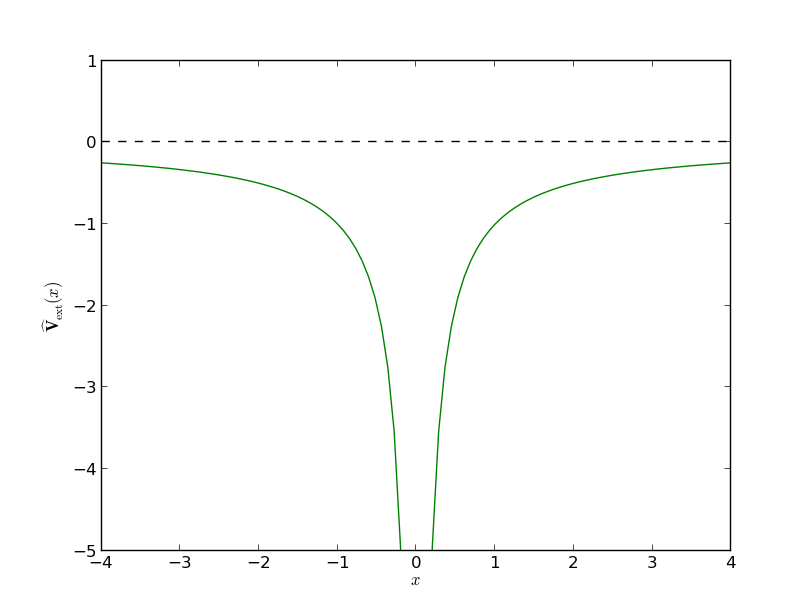
\includegraphics[scale=0.5]{../Graphics/Potentials/hydrogen.png}
  \caption{The single particle potential of hydrogen along the x-axis. The potential is spherically symmetric.}
  \label{fig:extPotHydrogen}
 \end{center}
\end{figure}

which results in the following single particle Hamiltonian

\begin{equation}
 \OP{h}_0(\mathbf{r}) = -\frac{1}{2}\nabla^2 - \frac{Z}{r}.
\end{equation}

The external potential is displayed in figure \ref{fig:extPotHydrogen}. The eigenfunctions of the Hamiltonian are

\begin{equation}
 \phi_{nlm}(r, \theta, \phi; Z) \propto r^l e^{-Zr/n}\left[L_{n-l-1}^{2l+1}\left(\frac{2r}{n}Z\right)\right] Y_l^m(\theta, \phi), \label{eq:hydrogenBasisComplex}
\end{equation}

where $L_{q-p}^p(x)$ is the \textit{associated Laguerre polynomial} and $Y_l^m(\theta, \phi)$ is called the \textit{spherical harmonics}, related to the \textit{associated Legendre functions} $P_l^m$ as following

\begin{equation}
 Y_l^m(\theta, \phi) \propto   P_l^m(\cos\theta)e^{im\phi}, \label{eq:spherHarm}
\end{equation}

In the current model, the principal quantum number $n$ together with $Z$ controls the energy level of the atom, 

\begin{equation}
 E(n; Z) = -\frac{Z^2}{2n^2}\label{eq:AtomNonIntEnergy}
\end{equation}

which implies that the energy levels are degenerate for all combinations of $l$ and $m$. For a given value of $n$, the allowed levels of the \textit{azimuthal} quantum number $l$ and the \textit{magnetic} quantum number $m$ is 

\begin{align*}
 n &= 1, 2, ... \\
 l &= 0, 1, ...\,, n-1 \\
 m &= -l, -l + 1, ...\,, l - 1, l
\end{align*}


A problem with the single particle basis of hydrogen is the complex terms in the spherical harmonics (see Eq.~(\ref{eq:spherHarm})). Complex bases will require the entire code to work in complex variables, which should be avoided if possible. For this reason, the spherical harmonics in Eq.~(\ref{eq:hydrogenBasisComplex}) are substituted with the real-valued \textit{solid harmonics} $S_l^m(r, \theta, \phi)$ \cite{SolidHarmonics}

\begin{align}
S_l^m(r, \theta, \phi) &= (-1)^m\frac{(1+m)!}{2}r^l\left[Y_l^m(\theta, \phi) + (-1)^m Y_l^{-m}(\theta, \phi)\right] \\
 &= (-1)^m r^{l} P_l^{|m|}(\cos\theta) \begin{cases} \cos m\phi & m \ge 0 \\ \sin|m|\phi &  m < 0, \end{cases}                                                                                                             
\end{align}

which yields the following real eigenfunctions

\begin{equation}
  \phi_{nlm}(r, \theta, \phi; k) \propto e^{-kr/n}\left[L_{n-l-1}^{2l+1}\left(\frac{2r}{n}k\right)\right] S_l^m(r, \theta, \phi) \equiv \phi_{nml}(\mathbf{r}), \label{eq:hydrogenBasisReal}
\end{equation}

where $k = \alpha Z$ is a scaled charge with $\alpha$ as a variational parameter chosen by methods described in Section \ref{sec:selectingOptVarPar}.

A set of quantum numbers $nlm$ is mapped to a single index $i$. A listing of all the single particle wave functions are given in Appendix \ref{appendix:SymPyHydro}.

\subsection{Atoms}

At atom is described as $N$ electrons surrounding a fixed nucleus of charge $Z=N$. The Hamiltonian consists of $N$ single particle Hamiltonians corresponding to the hydrogen case, in addition to the Coulomb interaction term

\begin{align}
 \OP{H}_{\mathrm{Atoms}} &= \sum_{i=1}^N \OP{h}_0(\mathbf{r}_i) + \sum_{i<j} \frac{1}{r_{ij}} \\
                         &= \sum_{i=1}^N \left[-\frac{1}{2}\nabla_i^2 - \frac{Z}{r_i}\right] + \sum_{i<j} \frac{1}{r_{ij}},
\end{align}

where $r_ij = |\mathbf{r}_i -\mathbf{r}_j|$. Excluding the Coulomb term, the Hamiltonian can be decoupled into single particle terms with energy

\begin{equation}
 E_0 = -\frac{Z^2}{2}\sum_{i=1}^N \frac{1}{n_i^2}.
\end{equation}

The Slater determinant is set up to fill the $N$ lowest lying states, that is, the $N$ states with lowest $n$\footnote{Keep in mind that only two particles can obtain the same state simultaneously.}, using the single particle orbitals from Eq.~(\ref{eq:hydrogenBasisReal}).

\subsection{Homonuclear Diatomic Molecules}

A homonuclear diatomic molecule consists of two atoms (diatomic molecule) of the same element (homonuclear) with charge $Z$, separated by a distance $R$. The origin is set between the atoms, which is then fixed at positions $\pm \mathbf{R}/2$. An electron at position $\mathbf{r}_i$ gets a contribution from both the cores as displayed in figure \ref{fig:dimolecules}. In addition, there is a repulsive Coulomb potential between the two cores equal to $Z^2/R$. The resulting Hamiltonian becomes

\begin{equation}
 \OP{H}_{\mathrm{Mol.}} = \sum_{i=1}^N \left[-\frac{1}{2}\nabla_i^2 + \frac{Z}{|\mathbf{r}_i + \mathbf{R}/2|} + \frac{Z}{|\mathbf{r}_i - \mathbf{R}/2|}\right] + \frac{Z^2}{R} + \sum_{i<j} \frac{1}{r_{ij}}
\end{equation}



\begin{figure}
 \begin{center}
  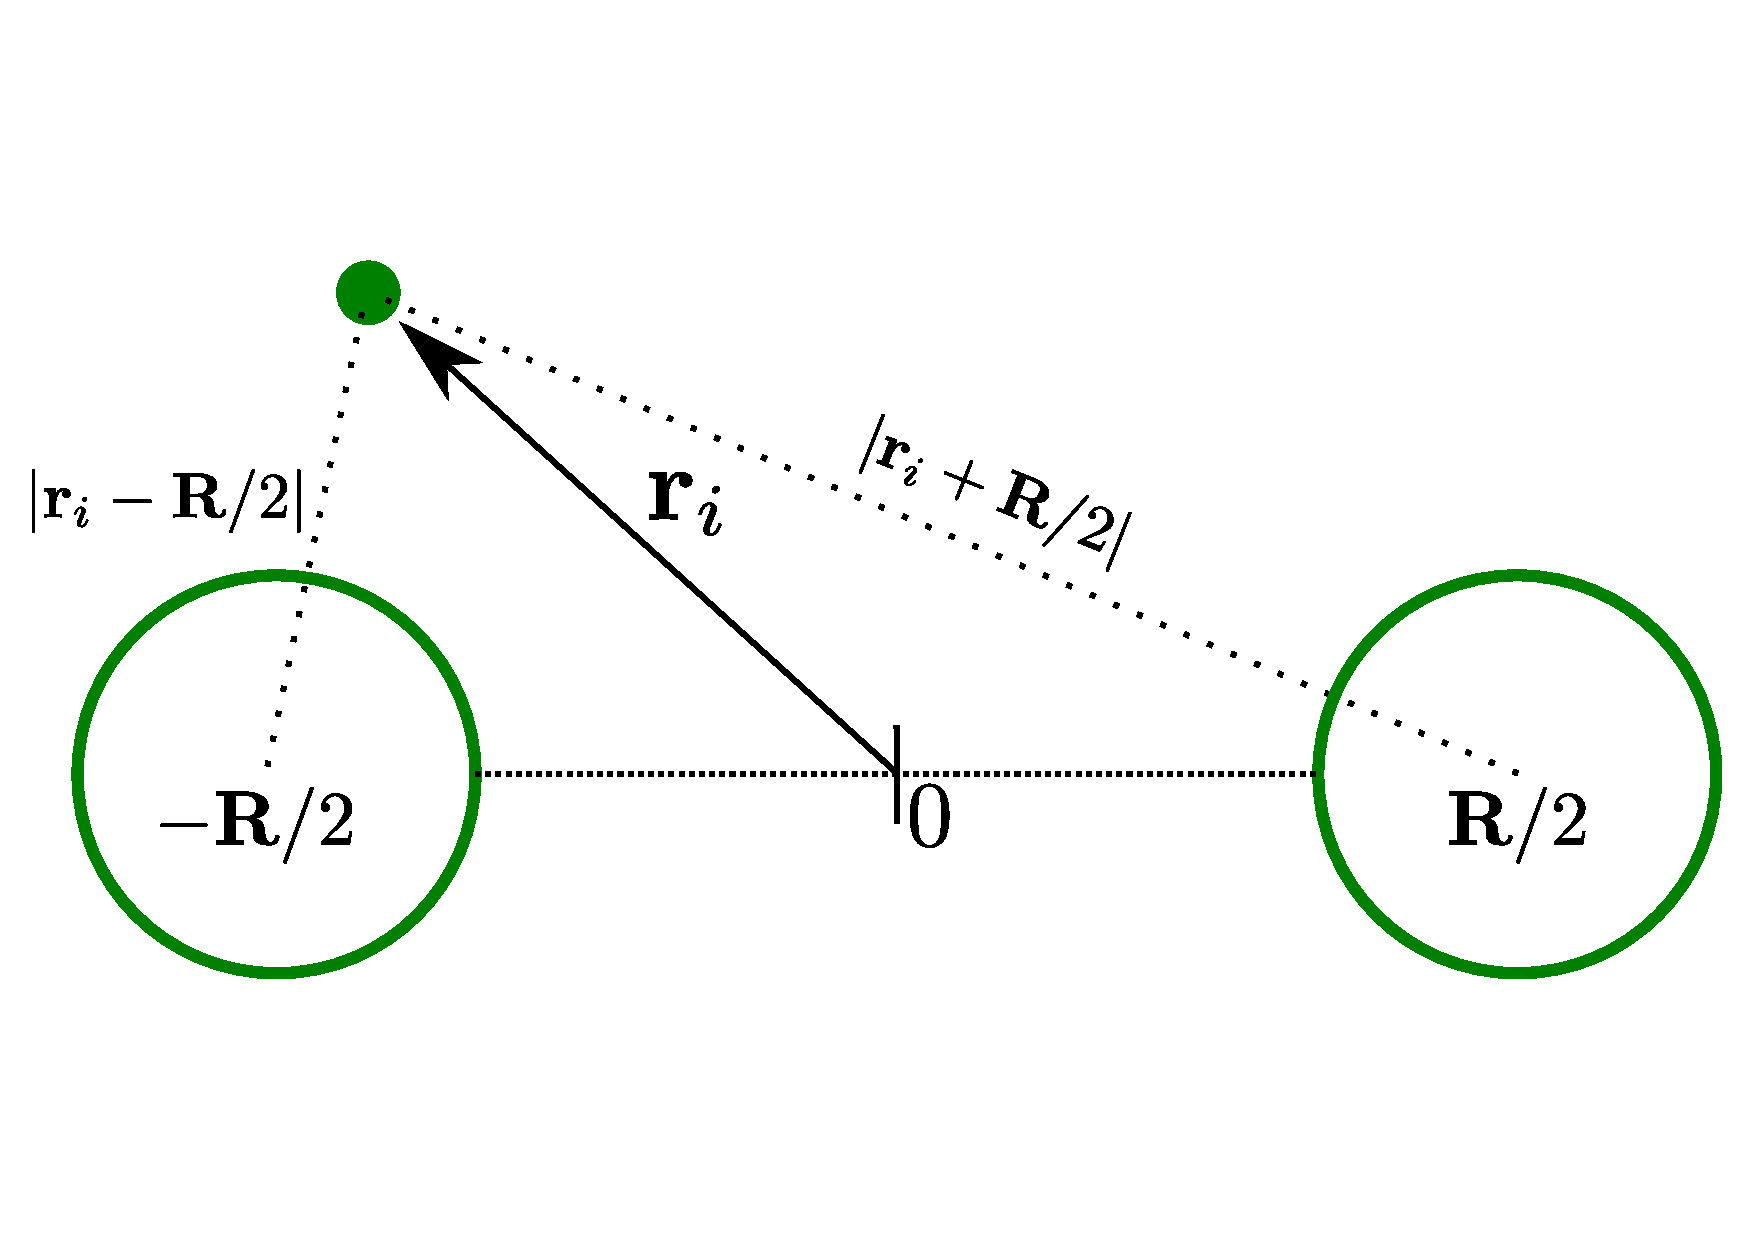
\includegraphics[scale=0.3]{../Graphics/Molecules.pdf}
  \caption{The model for the diatomic molecule used in this thesis. An electron at position $\mathbf{r}_i$ gets a potential energy contribution from both the cores equal to $Z/|\mathbf{r}_i + \mathbf{R}/2|$ and  $Z/|\mathbf{r}_i - \mathbf{R}/2|$, where Z is the charge of the nuclei (homonuclear).}
  \label{fig:dimolecules}
 \end{center}
\end{figure}


In order to transform the hydrogen eigenstates $\phi_{nml}^\mathrm{H}(\mathbf{r})$ (which is symmetric around a single nucleus) into molecular single particle states $\phi_{nml}^\pm (\mathbf{r}_i)$, a superposition of the two mono-nucleus wave functions are used

\begin{align}
 \phi_{nml}^+ (\mathbf{r}_i) &= \phi_{nml}^\mathrm{H}(\mathbf{r}_i + \mathbf{R}/2) + \phi_{nml}^\mathrm{H}(\mathbf{r}_i - \mathbf{R}/2) \\
 \phi_{nml}^- (\mathbf{r}_i) &= \phi_{nml}^\mathrm{H}(\mathbf{r}_i + \mathbf{R}/2) - \phi_{nml}^\mathrm{H}(\mathbf{r}_i - \mathbf{R}/2)
\end{align}

which reads ``electron surrounding first nucleus combined with electron surrounding second nucleus'' (recall that $\mathbf{r}_i \pm \mathbf{R}/2$ describes the vector from the nuclei to the electron). As seen from the equations above, there are necessarily two ways of doing this superposition: Adding and subtracting the states. It is easy to show that 

\begin{equation}
 \braket{\phi_{n'm'l'}^-}{\phi_{nml}^+} = 0
\end{equation}

which implies that these states form an expanded complete set of single particle states for the molecular system, resulting in a four-fold degeneracy in each set of quantum numbers $nml$. It is necessary to use both the positive and negative states in order to fit e.g. four electrons into $n=0$ for the case of lithium and beryllium. Using only positive or only negative states would result in a singular Slater determinant.

Using $\mathbf{R} = \left(R_x, R_y, R_z\right)$, $\mathbf{j} = (0, 1, 0)$, $\mathbf{r}_i = \left(x_i, y_i, z_i\right)$,  and the chain rule of derivation, the dell operator (in the $\mathbf{j}$-direction) becomes

\begin{align}
 \mathbf{j}\cdot \nabla_i \phi_{nml}^\pm (\mathbf{r}_i) &= \underbrace{\frac{\partial (y_i + R_y/2)}{\partial y_i}}_{1}\frac{\partial \phi_{nml}^\mathrm{H}(\mathbf{r}_i + \mathbf{R}/2)}{\partial (y_i + R_y/2)} \notag \\
  &\pm \underbrace{\frac{\partial (y_i - R_y/2)}{\partial y_i}}_{1}\frac{\partial \phi_{nml}^\mathrm{H}(\mathbf{r}_i - \mathbf{R}/2)}{\partial (y_i - R_y/2)} \notag\\
  &= \frac{\partial \phi_{nml}^\mathrm{H}(\mathbf{r}_i + \mathbf{R}/2)}{\partial (y_i + R_y/2)} \pm \frac{\partial \phi_{nml}^\mathrm{H}(\mathbf{r}_i - \mathbf{R}/2)}{\partial (y_i - R_y/2)} \notag\\
  &=  \frac{\partial \phi_{nml}^\mathrm{H}(\mathbf{\tilde R_i^+})}{\partial \tilde Y_i^+} \pm \frac{\partial \phi_{nml}^\mathrm{H}(\mathbf{\tilde R_i^-})}{\partial \tilde Y_i^-}, \label{eq:MoleculeWorksWithOldFunctions}
\end{align}

where $\mathbf{\tilde R_i^\pm} = \mathbf{r}_i \pm \mathbf{R}/2 = (\tilde X_i^\pm, \tilde Y_i^\pm, \tilde Z_i^\pm)$ represents the electron position in the two nuclei coordinate frames. Eq.~(\ref{eq:MoleculeWorksWithOldFunctions}) demonstrates that the closed form expressions from the atoms can be reused in the case of diatomic molecules; the functions in Appendix \ref{appendix:SymPyHydro} can simply be called  with $\mathbf{\tilde R_i^\pm}$ instead of $\mathbf{r}_i$ and then be either subtracted or added. This result holds for the Laplacian as well.

The non-interacting energy is equal to that of the regular atoms, however, now with a four-fold degeneracy and a charge equal to $N/2$.

\section{Quantum Dots}

\subsection{The Single Particle basis}

\subsection{2D and 3D Quantum Dots}

\subsection{Double-well Quantum Dots}








\part{Results}
%% \chapter{Implementation and Validation}

I will not discuss the specific implementations in this thesis. For a detailed description of specific functions etc., see the the actual code for comments. The concept of this chapter is to give insight about the ideas behind the implementation.  Long story short, alot of hard work has been put into deep object orientation (for details, see Section~\ref{sec:OO}) in order to combine the different building blocks of QMC-methods in a natural and coherent way. As with all big coding projects, a major part of development went into planning and structuring.

\section{Structure and Implementation}
\label{sec:StructureandImplementation}

In QMC, Quantum Mechanics, and even physics in general, there are natural ways of decoupling the code in order to create a bridge between physics and code. Gathering data into objects representing physical concept to which a reader can relate increases the overall readability of the code. It also dramatically decreases the time it takes to implement or debug new methods, since mathematical intuition can be used in order to trace certain behaviours back to the source \footnote{For instance, if something is wrong with the sampling rule, a random walker might behave weird. The natural starting point of debugging is then the object in which the sampling rules are set. In the case of this thesis, this is the Sampling class containing a Diffusion object.}. Another reason is to generalize the code for several different cases, without having to rewrite or mess up anything (see the PotionGame example in Section~\ref{sec:PotionGame}).

\subsection{Methods used for Increasing Readability and Overall Structure}


As an example, the contents of the \verb+Walker+ class in Table ~\ref{tab:walkerClassMembers}. The idea behind this structure is that whenever we need a new walker in e.g. DMC, all we need to do is to create a new instance of \verb+Walker+. Deleting a walker is just as clean. A function which requires access to several elements from Table~\ref{tab:walkerClassMembers} now only requires one argument, namely the walker of interest. Let us look at an example


\vspace{0.5 cm}
\begin{lstlisting}
DMC::DMC(...) {

    ...
 
    original_walkers = new Walker*[spesify a number of walkers];
    
    ...

}
\end{lstlisting}


\begin{lstlisting}
void DMC::initialize() {

    ...

    //Initializing active walkers
    for (int k = 0; k < n_w; k++){
        original_walkers[k] = new Walker(n_p, dim);
    }
    
    //Seting trial position of active walkers
    ...

    //Calculating and storing energies of active walkers
    for (int k = 0; k < n_w; k++) {
        calculate_energy_necessities(original_walkers[k]);
        original_walkers[k]->set_E(calculate_local_energy(original_walkers[k]));
    }

    ...

}
\end{lstlisting}

\begin{table}

 \begin{center}

 \begin{tabular}{|c l l|}
 \hline
 Type & Name & Description \\
 
 \hline
 \hline
 
 \verb+mat+         & \verb+r+             & The position.\\

 \hline
 \hline
 
 \verb+mat+         & \verb+r_rel+         & The relative positions.\\
 \verb+rowvec+      & \verb+ r2+           & The squared positions. \\
 \verb+mat+         & \verb+phi+           & The last evaluated single particle orbitals. \\
 \verb+field<mat>+  & \verb+dell_phi+      & The last evaluated gradients of the single particle orbitals. \\
 \verb+cube+        & \verb+dJ+            & The last evaluated terms of the jastrow factor derivatives. \\
 \verb+mat+         & \verb+spatial_grad+  & The gradient of the uncorrelated wave function.\\
 \verb+mat+         & \verb+jast_grad+     & The gradient of the Jastrow factor.\\
 \verb+mat+         & \verb+inv+           & The inverse of the slater matrix.\\
 \verb+mat+         & \verb+qforce+        & The quantum force.\\
 
 \hline 
 \hline
 
 \verb+double+      & \verb+spatial_ratio+ & The current ratio between this walker and another walker.\\
 \verb+double+      & \verb+value+         & The value of the wave function.\\
 \verb+double+      & \verb+lapl_sum+      & The full Laplacian of the wave function.\\
 \verb+double+      & \verb+E+             & The energy of the walker. \\
 \verb+bool+        & \verb+is_murdered+   & A flag for the DMC brancing algorithm. \\
 \hline 
 \end{tabular}
 
 \caption{Description of the members of the Walker class. All matrices holds information on all particles.
The second block corresponds to vectors kept in memory to avoid expensive recalulation. The third block corresponds to  scalar values calculated and kept in memory for later use or control.}
 \label{tab:walkerClassMembers}
 
 \end{center}
\end{table}

Initializing new walkers is, as seen above, unproblematic. Calculating values in the machinery now always involves a corresponding walker. For instance, when looping over walkers in DMC, the amount of juggling is reduced to nothing; all you need to do is to loop over a vector of walkers. This walker can then be sent to any function, resulting in code like e.g.

\vspace{0.5cm}
\begin{lstlisting}
double Coulomb::get_pot_E(const Walker* walker) const {
    
    double e_coulomb = 0;

    for (int i = 0; i < n_p - 1; i++) {
        for (int j = i + 1; j < n_p; j++) {
            e_coulomb += 1 / walker->r_rel(i, j);
        }
    }

    return e_coulomb;
}
\end{lstlisting}

The alternative to the code above is to juggle one relative position matrix per walker, ruining both the readability and the overall structure of the code. Another upside to this way of structuring, is that we can tie the source code and the method description closer together. Look at VMC as an example. VMC uses a walker and a trial walker. 

\vspace{0.5cm}
\begin{lstlisting}
void VMC::initialize() {
    
    ...

    sampling->set_trial_pos(original_walker);
    copy_walker(original_walker, trial_walker);
    
    ...
    
}

\end{lstlisting}

Another example where object orientation dramatically increases the readability of the code is the interplay between the Sampling- and Diffusion-class. From \textbf{REF TO THEORY} we know that if we use importance sampling, the diffusion follows the Fokker-Planck equation (Eq.~\textbf{CITE EQ FOKKERPLANCK}). The implementation is as follows:

\vspace{0.5cm}
\begin{lstlisting}
Importance::Importance(GeneralParams & gP)
: Sampling(gP.n_p, gP.dim) {

    diffusion = new Fokker_Planck(n_p, dim, gP.random_seed);

}
\end{lstlisting}


\subsection{Methods for Generalizing the Code}

The importance sampling constructor serves as a good example in this case as well. A \verb+Sampling+ object type might be an instance of \verb+Importance+ or \verb+Brute_Force+, however, we do not need to know this in order to abstractly describe how to diffuse a walker. We do not even need to know whether we are doing VMC or DMC. All we need to know is that the \verb+Diffusion+ object within the sampling holds the rules we need once the correct objects are in place. This is reflected in the following code:

\vspace{0.5cm}
\begin{lstlisting}
void Sampling::update_pos(const Walker* walker_pre, Walker* walker_post, int particle) const {

    for (int j = 0; j < dim; j++) {
        walker_post->r(particle, j) = walker_pre->r(particle, j)
                + diffusion->get_new_pos(walker_pre, particle, j);
    }

    //more updates through jastrow pointers etc.
    ...

}
\end{lstlisting}

\begin{lstlisting}
double Diffusion::get_new_pos(const Walker* walker, int i, int j) {
    return gaussian_deviate(&random_seed) * std;
}

double Simple::get_new_pos(const Walker* walker, int i, int j) {
    return Diffusion::get_new_pos(walker, i, j);
}

double Fokker_Planck::get_new_pos(const Walker* walker, int i, int j) {
    return D * timestep * walker->qforce(i, j) + Diffusion::get_new_pos(walker, i, j);
}
\end{lstlisting}

This use of polymorphism (as described in Section \ref{sec:typeCastPoly}) is widely used throughout the code to generalize it. As a goal, the idea was to produce a code with the following generalizations:

\begin{itemize}
 \item As many as possible functions should be written generally for DMC and VMC.
 \item Objects should not assume the type of any sub-classed object except its own, unless the type is directly implied (importance sampling implies Fokker-Planck diffusion), i.e., deep polymorphism.
\end{itemize}

This puts a series of constraints on the code; it should be general for (in any combination):

\begin{enumerate}[label=(\roman{*}), ref=(\roman{*})]
\item No trailing if-tests or flags handling switched cases. A single test in the main file decides everything once and for all. 
\item Importance- and Brute Force-sampling.
\item Numerical or closed form expressions for the kinetic energy and quantum force.
\item Fermions and Bosons.
\item Any choice of single particle basis, included expanded bases.
\item Functionality to add any combination of any potential.

\end{enumerate}


\subsubsection{Constraints (i) - (iv)}

As mentioned previously, \verb+QMC+ holds an object of type \verb+Sampling+, which contains all the general functions for diffusing particles and how to sample them. It also ensures that the walker holds the necessary data in order to continue the sampling, e.g. the Quantum Force if we do importance sampling. This is achieved by having a pure virtual function \verb+get_necessities+, which is overrided by the subclasses \verb+Importance+ and \verb+Brute_Force+. In other words: The class structure is set up in such a way that the distinct parts which needs to be general are separated. Polymorphism takes care of the distinction, hence no if-tests are required. Below follows a part of the code illustrating this; the code for copying walkers, calculating energy necessities etc. follows the same idea.

\vspace{0.5cm}
\begin{lstlisting}
void Sampling::update_pos(const Walker* walker_pre, Walker* walker_post, int particle) const {

    //Positions and orbitals are updated for the particle at hand
    ...

    //updates the inverse slater in case of a fermion system
    qmc->get_system_ptr()->calc_for_newpos(walker_pre, walker_post, particle);

    //pure virtual function. Function will update quantum force if importance sampling.
    update_necessities(walker_pre, walker_post, particle);

}
\end{lstlisting}

In the case of numerical energy calculations, the function which evaluates the gradients can be set to a general numerical function (assuming the standard single particle orbitals are implemented). If the closed form expressions are implemented, these can be accessed directly instead. Fermions and bosons have different implementations of e.g. the spatial ratio of a wavefunction.


\subsubsection{Constraint (v)}

A single particle orbital is nothing but a function of a walker's coordinates and variational parameters.  An if-test hierarchy on the Quantum Number is the simplest way to implement a single particle basis, however, they can all be avoided using polymorphism. The class \verb+BasisFunctions+ represents an abstract function, which can takes on input a walker and evaluates an arbitrary expression. A subclass will hold the specific implementation, e.g. the first excited level of a harmonic oscillator.

\vspace{0.5cm}
\begin{lstlisting}
class BasisFunctions {
public:
    BasisFunctions();
    
    virtual double eval(const Walker* walker, int i) = 0;
};

double alphaHO_3::eval(const Walker* walker, int i) {
    
    //4*k2*y2 - 2
    H = 4*(*k2)*walker->r(i, 1)*walker->r(i, 1) - 2;
    return H * (*exp_factor);
    
}
\end{lstlisting}

These functions are loaded into an array representing the single particle basis in the \verb+Orbitals+ class' constructor.

\vspace{0.5cm}
\begin{lstlisting}
AlphaHarmonicOscillator::AlphaHarmonicOscillator(GeneralParams & gP, VariationalParams & vP)
: Orbitals(gP.n_p, gP.dim) {

    //Creating pointers in order to link the Orbital and BasisFunction parameters.
    this->alpha = new double();
    this->k = new double();
    this->k2 = new double();
    this->exp_factor = new double();

    this->w = gP.systemConstant;
    set_parameter(vP.alpha, 0);
    get_qnums();

    basis_functions[0] = new alphaHO_0(k, k2, exp_factor);
    basis_functions[1] = new alphaHO_1(k, k2, exp_factor);
    basis_functions[2] = new alphaHO_2(k, k2, exp_factor);
    basis_functions[3] = new alphaHO_3(k, k2, exp_factor);
    ...
    
\end{lstlisting}

All orbital files are generated automatically by a Python-script. The reasoning behind the unset pointers are to create a link between the parameters in \verb+BasisFunctions+ and \verb+Orbitals+, such that we do not have to change the value in all of the basis function objects (60 for 30 particles), we simply have to change the value in the orbitals class and the rest will follow.

With this rigid setup, evaluating orbitals can now we done in the following manner (similar for the gradient and Laplace)

\vspace{0.5cm}
\begin{lstlisting}
virtual double phi(const Walker* walker, int particle, int q_num) {
    return basis_functions[q_num]->eval(walker, particle);
}
\end{lstlisting}

The reason why \verb+phi+ is a virtual function, is so that the \verb+ExpandedBasis+ class can override it. With this systematic setup of single particle orbitals, it is very simple and intuitive to implement the expanded basis functionality

\vspace{0.5cm}
\begin{lstlisting}[language=C++]
class ExpandedBasis : public Orbitals {

...

protected:

    int basis_size;
    arma::mat coeffs;
    Orbitals* basis;

};

ExpandedBasis::ExpandedBasis(GeneralParams & gp, Orbitals* basis, int basis_size, std::string coeffPath)
: Orbitals(gp.n_p, gp.dim) {

    this->basis = basis;
    this->basis_size = basis_size;
    coeffs = arma::zeros<arma::mat > (n2, basis_size);

    //read coefficients

}

\end{lstlisting}

The expanded basis class is implemented as a subclass to the original orbital class, however, it is designed to work along side it. Instead of a list of orbital basis functions, it holds a \verb+Orbital+ object, containing the basis in which we want to expand, alongside a matrix containing the coefficients of expansion. Implementing the new single particle functions is simply done by virtual function overriding as below: 

\vspace{0.5cm}
\begin{lstlisting}

double ExpandedBasis::phi(const Walker* walker, int particle, int q_num) {

    double value = 0;
    for (int m = 0; m < basis_size; m++) {
        value += coeffs(particle, m) * basis->phi(walker, particle, m);
    }

    return value;

}
\end{lstlisting}

And of course similarly for the gradient and Laplace. The expression is very close to the raw mathematical description of a basis expansion. 

\subsubsection{Constraint (vi)}

When we are loading a set of single particle states, we are loading those who best match the given Hamiltonian of our system. For quantum dots, we load harmonic oscillator states, for atoms we load hydrogen states and so on. By having great flexibility in both the Hamiltonian and the basis functions means the code is easily adaptable to other systems. The flexibility of the potential class is already discussed in Section \ref{sec:typeCastPoly}.

The complete list of classes working in the same way (iteration over loaded elements, no if-tests) is


\begin{listliketab}
\storestyleof{itemize}
 \begin{tabular}{l l}
  \textbullet \,\verb+Potential+         & See section \ref{sec:typeCastPoly} for detials. \\
  \textbullet \,\verb+ErrorEstimator+:   & Initialized to \verb+Blocking+ or \verb+SimpleVar+. Samples data.\\
  \textbullet \,\verb+OutputHandler+:    & Saves specified data to a specified file, e.g. \verb+stdoutDMC+.\\
 \end{tabular}
\end{listliketab}


Creating optimized and general code takes longer to develop, but pays off when it comes to later implementations of extensions to the library.

\subsection{Visualization}
DCVIZ?

\section{Performance Optimizations}

\subsection{RAM use}

the RAM use of VMC is close to nothing; we only have two walkers with each their set of matrices. However, DMC has the potential to use a lot of RAM, as thousands of walkers are allocated. The walkers account for close to all of the RAM used by the methods, as the rest of the framework consist only of a small amount of doubles (8 bytes) and integers (4 bytes). A short analysis of the RAM spent per \verb+Walker+ object yields

\begin{listliketab}
\storestyleof{itemize}
 \begin{tabular}{l l}
  \textbullet 1 boolean                                        & 1 byte                                \\
  \textbullet 3 integers                                       & 12 bytes                              \\
  \textbullet 3 doubles                                        & 24 bytes                              \\
  \textbullet 4 \verb+n_p+ $\times$ \verb+dim+ matrices        & 32 \verb+n_p+ $\cdot$ \verb+dim+ bytes\\
  \textbullet 1 \verb+n_p+ $\times$ \verb+n_p+ matrix        & 8 \verb+n_p+ $\cdot$ \verb+n_p+ bytes \\
  \textbullet 2 \verb+n_p+ $\times$ \verb+n_p/2+ matrices        & 4 \verb+n_p+ $\cdot$ \verb+n_p+ bytes \\
  \textbullet 1 array of length \verb+n_p+                     & 8 \verb+n_p+ bytes                    \\
  \textbullet 1 field of length \verb+n_p+                     & 8 \verb+n_p+ bytes                    \\
  \textbullet 1 \verb+n_p+ $\times$ \verb+n_p/2+ $\times$ \verb+dim+ field & 8 \verb+n_p+ bytes                    \\
  \textbullet 1 \verb+n_p+ $\times$ \verb+n_p+ $\times$ \verb+dim+ cube & 8 \verb+n_p+ bytes\\
  Total:                                                       & 37 + 32 \verb+n_p+ $\cdot$ \verb+dim+ + 12 \verb+n_p+ $\cdot$ \verb+n_p+ + 8 \verb+n_p+ bytes \\
 \end{tabular}
\end{listliketab}

For VMC with 30 particles and quantum dots in 2 dimensions this gives a walker RAM usage of 25 kB, which is practically nothing. For DMC however, we have e.g. 1000 active walkers and 4000 inactive. The inactive ones can be left uninitialized, saving the RAM of all matrix initializations (37 RAM per walker). 

In Figure~\ref{FIG:RAMusageDMC} we see how the RAM usage in a typical DMC calculation scales with the number of particles. For 30 particles, we have approximately 60 MB of RAM spent on walkers. This is still practically nothing compared to the available RAM on modern computers (minimum 2 GB).

\begin{figure}
\label{FIG:RAMusageDMC}
 \begin{center}
  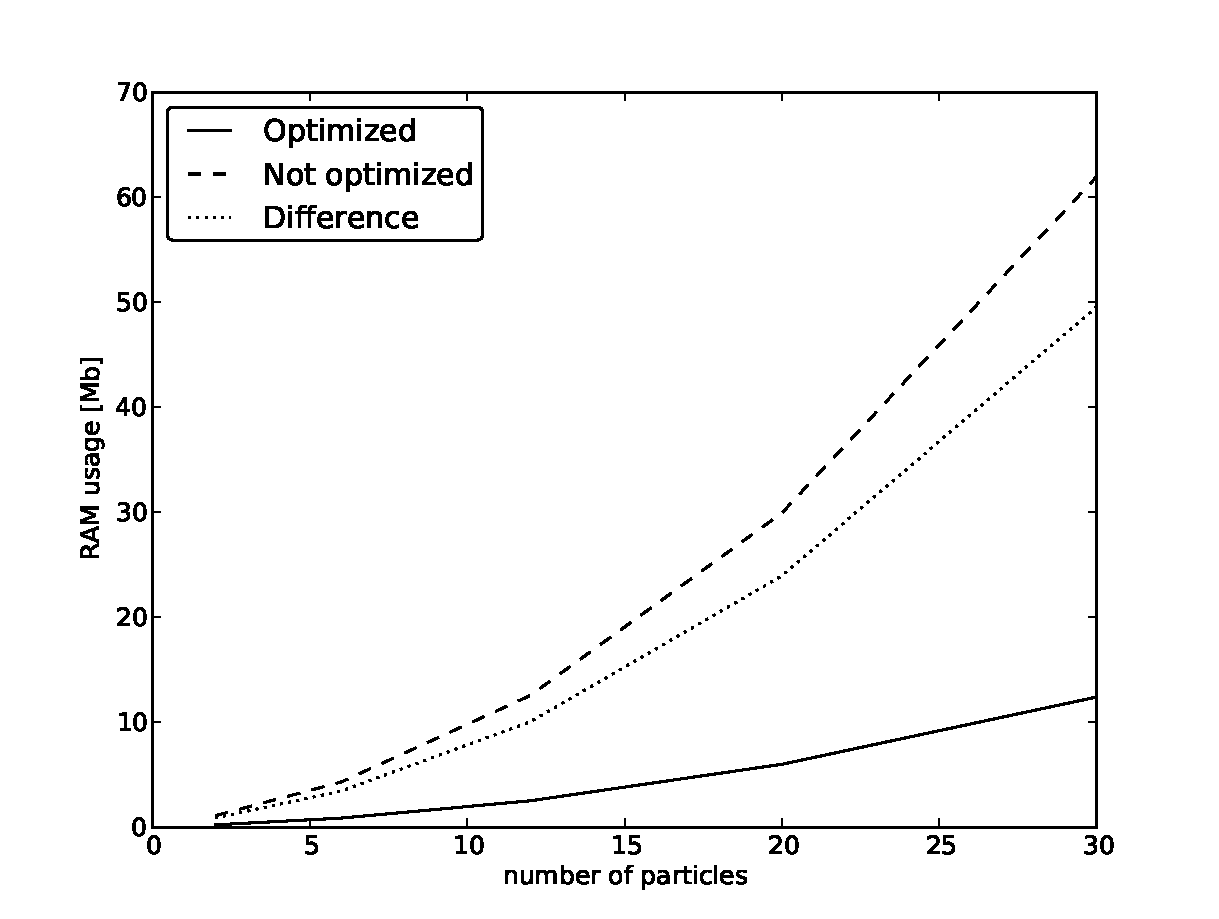
\includegraphics[scale=0.75]{../Graphics/RAMusagePrWalker.pdf}
  \caption{Number of particles vs. the theoretical RAM usage in a typical DMC run for the optimized and unoptimized case. Calculated for two dimensions, 1000 active walkers and 5000 inactive.}
 \end{center}
\end{figure}

The conclusion stands that as long as there are no memory leaks, time spent optimizing the memory use is time wasted. Memory optimizations might damage the readability, so the code was left more or less unoptimized in this part.

\subsection{CPU-time}
Looking at Table \ref{tab:walkerClassMembers}, the only thing we have to store in order for the machinery to work is the position matrix. Every other matrix is initialized to optimize CPU time.

During a Quantum Monte Carlo sampling process, certain values, such as the relative distances, are used to calculate quantities such as the energy. The most brute force way of handling situations like this is to calculate everything at the time it is needed. However, once a diffusion step is made,we use the same relative distances both in the Jastrow factor and its gradient. Calculating them twice is a waste of time. We can instead store them in a matrix, and access this matrix in both functions:

\[
r_{rel} = r_{rel}^T = \left( \begin{array}{ccccc}
0 & r_{12} & r_{13} & \cdots & r_{1N} \\
 & 0 & r_{23} & \cdots & r_{2N}  \\
 &  & \ddots & \ddots & \vdots \\
 & \cdots &  & 0 & r_{(N-1)N} \\
 &  &  &  & 0\end{array} \right).
\]

Another upside with this way of storing the relative distances, is that moving particle $i$ in our code, only changes the $i$'th row in the matrix, and therefore we need only to recalculate \textit{N} elements (\textit{N} being the number of particles in our system). For the same reason, storing the gradients, Laplacian sums and the squared radii is matrices also optimize the code. 

Having closed form expressions for the gradients and Laplacians for the different parts of the wave function is another source of dramatic speed-up. The local kinetic energy ($(E_k)_L$) and the Quantum Force ($\mathbf{F}_i$) can be expressed in terms of the separate parts of the wave function:

\begin{eqnarray}
(E_k)_L &=& -\frac{1}{2}\frac{1}{\psi_T}\nabla_i^2 \psi_T \\
&=& -\frac{1}{2}\frac{1}{|S|\psi_C}\nabla_i^2(|S|\psi_C) \nonumber\\
&=& -\frac{1}{2}\frac{1}{|S|\psi_C} \nabla_i \left(\psi_C\nabla_i |S| + |S|\nabla_i \psi_C\right)\nonumber  \\
&=& -\frac{1}{2}\Big[\frac{1}{\psi_C}\nabla_i^2 \psi_C + \frac{2}{|S|\psi_C}\nabla_i|S|\cdot\nabla_i\psi_C \nonumber\\
&& \qquad\qquad\qquad\,\,+\frac{1}{|S|}\nabla_i^2 |S|\Big].\nonumber 
\label{eq:kinetic_analytic}
\end{eqnarray}

\begin{eqnarray}
 \mathbf{F}_i &=& \frac{2}{|S|\psi_C}\nabla_i( |S|\psi_C) \\
&=& 2\left(\frac{1}{\psi_C}\nabla_i \psi_C + \frac{1}{|S|}\nabla_i |S|\right),\nonumber
\label{eq:QF}
\end{eqnarray}
where $i$ denotes particle number, and $|S|$ and $\psi_C$ are respectively the spatial wave function and the Jastrow factor.

For Fermions, it can be shown that we have the following relations for the Slater determinant\cite{larseivind}:

\begin{eqnarray}
 \frac{1}{|S|}\nabla_i |S| &=& \displaystyle\sum_{j=1}^n \nabla_i \phi_j(\vec r_i)S^{-1}_{ji} \\ 
\frac{1}{|S|}\nabla^2_i |S| &=& \displaystyle\sum_{j=1}^n \nabla^2_i \phi_j(\vec r_i)S^{-1}_{ji},\nonumber
\label{eq:grad_lapl_S}
\end{eqnarray}
where $S^{-1}$ is the inverse of the Slater matrix, and $n$ is the dimensionality of the Slater matrix, in our case $n=N/2$, where $N$ is the number of electrons. $\phi_j(\vec r_i)$ are the single-particle basis functions, where $j$ denotes the quantum numbers. For example $j=0$ is the ground state, $j=1$ first excited state and so on. 

These values of the gradient and Laplacian of the single-particle wave functions needs to be tabulated. Most of the single particle bases used are expressed using simple mathematics, such as Hermite polynomials for the case of harmonic oscillator, and the derivatives can therefore be calculated pretty easily. 

Calculating an inverse does not seem to optimize much. However, we can run an updating algorithm for the inverse, which ends up saving a lot of time. The ratio of the spatial determinants can also be expressed using this inverse\cite{larseivind}. This means that no explicit wave function calculation is needed (we can calculate the ratio between two Jastrow factors without problem). The expression for the ratio in terms of the inverse is
\begin{equation}
 R_S = \displaystyle\sum_{j=1}^n \phi_j({\vec r}_{i,\mathrm{new}})S^{-1}_{ji}(\vec r_\mathrm{old}),
\label{eq:Ratio}
\end{equation}
where $i$ is the particle being moved.

In the case of $s=\frac{1}{2}$-Fermions, the code holds two slater determinants (spin up and down); we need two inverse matrices. All if-tests on whether or not to access spin up or down is however avoided by merging the two inverse matrices into one augmented matrix

\[
 S^{-1} = \left[S^{-1}_\uparrow S^{-1}_\downarrow\right].
\]

\noindent
This way of storing the data completely removes the need of if-tests on spin.

Updating the inverse matrix can be done once we got the new position and the ratio

\begin{eqnarray}
 S^{-1}_{kj}(\vec r_\mathrm{new})  = \left\{ 
\begin{array}{l l}
  S^{-1}_{kj}(\vec r_\mathrm{old}) - \frac{1}{R_S}S^{-1}_{ki}(\vec r_\mathrm{old})\displaystyle\sum_{l=1}^{n} \phi_{l}(\vec r_{i,\,\mathrm{new}})  S^{-1}_{lj}(\vec r_\mathrm{old}) &\qquad \mbox{$j \neq i$} \\
 \frac{1}{R_S}S^{-1}_{ki}(\vec r_\mathrm{old})  &\qquad \mbox{$j=i$}
\end{array} \right.
\label{eq:Update_inv}
\end{eqnarray}


Equal expressions like the the ones listed in Eq.~(\ref{eq:grad_lapl_S}) can be found for the case of the Pade-Jastrow factor as well:

\begin{eqnarray}
 \frac{1}{\psi_C^{PJ}}\nabla_i \psi_C^{PJ} &=& \displaystyle\sum_{j\ne i} \frac{\vec r_{ij}}{r_{ij}}\frac{a_{ij}}{(1+\beta r_{ij})^2} \\
\label{eq:grad_jast}
 \frac{1}{\psi_C^{PJ}}\nabla_i^2 \psi_C^{PJ} &=& \left|\frac{1}{\psi_C^{PJ}}\nabla_i \psi_C^{PJ}\right|^2 + 2\displaystyle\sum_{i < j} \frac{a_{ij}(1 - \beta r_{ij})}{r_{ij}(1 + \beta r_{ij})^3}. \nonumber
\label{eq:lapl_jastrow}
\end{eqnarray}

Notice that $a_{ij}$ is written as a matrix element. If we were to calculate $a$ for every single run in the loop, the double if-tests would drain a lot of CPU time. Prior to the sampling, in the \verb+Jastrow::initialize+ function, the values of $a$ are generated once and for all and stored in a matrix. This matrix remains unchanged throughout the entire sampling, and no if-tests are necessary.

For the simplest case of single particle harmonic oscillator basis functions (Eq.~(\textbf{REF OSC BASIS}), the expressions for the derivatives of the wave function with respect to the variational parameters is
\begin{eqnarray}
\frac{1}{\psi_T}\frac{\partial\psi_T}{\partial\alpha} &=& -\frac{1}{2}\omega\displaystyle\sum_{i=1}^N r_i^2, \\
\frac{1}{\psi_T}\frac{\partial\psi_T}{\partial\beta} &=& -\displaystyle\sum_{i<j}\frac{a_{ij}r_{ij}^2}{(1+\beta r_{ij})^2}.
\label{eq:CGM_derivatives}
\end{eqnarray}

which can be used to speed up the process of minimizing.


Optimization (without approximations) is all about not calculating more than you have to. Calculating gradients is the part of the code which require the most CPU time. The most time consuming functions is the gradients. Looking at Eq.~(\ref{eq:grad_lapl_S}) this comes as no surprise; the single particle wave functions contain a call to the exponential function, which is terribly slow and needs to be deadly accurate. The time consumption in the Jastrow gradient arise from the fact that once a particle is moved, the entire gradient changes. 

\section{Validation}

things should not be wrong. It is bad.


test:
\newpage
\begin{table}
\begin{center}
\label{tab:DMCRes}
\begin{tabular}{cc|cccc}
    N     & $\omega$ & $\mathrm{E_{VMC}}$ & $\mathrm{E_{DMC}}$ & $\alpha$ & $\beta$  \\
\hline
    2     &   0.28   & 1.02197  &  1.0216  & 0.970202 & 0.254158 \\
          &   0.5    & 1.66023  & 1.65994  & 0.981901 & 0.312174 \\
          &   1.0    & 3.00054  & 3.00002  & 0.988761 & 0.398956 \\
    6     &   0.28   & 7.62259  & 7.59967  & 0.87322  & 0.322838 \\
          &   0.5    & 11.8092  & 11.7845  & 0.896501 & 0.411444 \\
          &   1.0    & 20.1896  & 20.1606  & 0.920368 & 0.55734  \\
    12    &   0.28   & 25.7088  & 25.63814 & 0.797355 & 0.365122 \\
          &   0.5    & 39.2395  & 39.15974 & 0.859145 & 0.481956 \\
          &   1.0    & 65.7958  & 65.70032 & 0.873605 & 0.656703 \\
\end{tabular}
\caption{J. Hogberget}
\end{center}
\end{table}

\begin{table}
\begin{center}
\label{tab:LohneRes}
\begin{tabular}{cc|cccc}
    N     & $\omega$ & $\mathrm{E_{DMC}}$  \\
\hline
    2     &   0.28   &  N/A     \\
          &   0.5    & 1.65975(2)  \\
          &   1.0    &  3.00000(3) \\
    6     &   0.28   &   7.6001(1) \\
          &   0.5    &  11.7888(2) \\
          &   1.0    &  20.1597(2) \\
    12    &   0.28   &  25.6356(1) \\
          &   0.5    &  39.159(1)  \\
          &   1.0    &  65.700(1)  \\
\end{tabular}
\caption{M. Pedersen Lohne et al.}
\end{center}
\end{table}

\begin{table}
\begin{center}
\label{tab:noColValid}
\begin{tabular}{cc|ccc}
    N     & $\omega$ & $\mathrm{E_{VMC}}$ & $\mathrm{E_{DMC}}$ & $\alpha$ \\
\hline
    2     &   0.5    &   1.0    &   1.0    &   1.0    \\
          &   1.0    &   2.0    &   2.0    &   1.0    \\
    6     &   0.5    &   5.0    &   5.0    &   1.0    \\
          &   1.0    &   10.0   &   10.0   &   1.0    \\
    12    &   0.5    &   14.0   &   14.0   &   1.0    \\
          &   1.0    &   28.0   &   28.0   &   1.0    \\
    20    &   0.5    &   30.0   &   30.0   &   1.0    \\
          &   1.0    &   60.0   &   60.0   &   1.0    \\
    30    &   0.5    &   55.0   &   55.0   &   1.0    \\
          &   1.0    &  110.0   &  110.0   &   1.0    \\
\end{tabular}
\caption{}
\end{center}
\end{table}



\chapter{Results}

\section{Optimization Results}
\label{sec:optRes}

The optimization results listed in this section are estimated using a 30-particle two-dimensional quantum dot as reference system.

Profiling the code revealed that $\sim99\%$ of the run time was spent diffusing the particles, that is, spent in the function \verb+QMC::diffuse_walker+. Variational Monte-Carlo (VMC), Diffusion Monte-Carlo (DMC), and Adaptive Stochastic Gradient Descent (ASGD) all rely heavily on the diffusion of particles, hence the parts of the code which do not involve diffusion walkers were neglected in the optimization process; it is a waste of time to optimize something which accounts for less than one percent of the run time.  

The profiling tool of choice was \textit{KCacheGrind}, which is available for free at the Ubuntu Software Center. KCacheGrind lists relative time spent in functions graphically in blocks whose sizes are proportional to the time spent inside the functions, much like standard hard drive listing software does with files and file sizes.

Optimizations discussed in Chapter \ref{ch:optAndGen} which are not mentioned in the following sections were considered standard implementations, and were thus implemented prior to the optimization process.

\subsubsection{Storing the Slater matrix}

This optimization is described in detail in Section \ref{sec:storeSlater}. In addition to storing the Slater matrix, the calculation of $\mathbf{\tilde I}$ from the inverse updating algorithm in Eq.~(\ref{eq:Itilde}) was taken outside of the main loops.

The percentages listed in the following table represent the ratio between the total time spent inside the given function and the total run time. 

\begin{tabular}{ll}
 \verb+Orbitals::phi+ & \\
 \hline\hline
 Relative run time used prior to optimization & 80.88\% \\
 Relative run time used after optimization    & 8.2\% \\
 \hline
 Relative function speedup                   & 9.86
\end{tabular}

The speedup comes not as a result of optimizations within the function itself, but rather as a result of far less calls to the function. If $\mathbf{\tilde I}$ was calculated outside of the main loops in the first place, the speedup would be far less significant. 


\subsubsection{Optimized Jastrow gradient}

The optimization described in this section is discussed in detail in Section \ref{sec:optJastGrad}.

The percentages listed in the following table represent the ratio between the total time spent inside the given functions and the total run time. 

\begin{tabular}{ll}
 \verb+Jastrow::get_grad+ \& \verb+Jastrow::calc_dJ+ & \\
 \hline\hline
 Relative run time used prior to optimization & 40\% \\
 Relative run time used after optimization    & 5.24\% \\
 \hline
 Relative function speedup                   & 7.63
\end{tabular}

Exploiting the symmetries of the Padé Jastrow gradient, in addition to calculating the new gradient based on the old, are in other words extremely efficient. Keep in mind that these results are for a high number of particles. For two particles, this optimization would not matter at all.

\subsubsection{Storing the orbital derivatives}

This optimization is covered in detail in Section \ref{sec:storeSlater}. Much like for the Slater matrix, the optimization in this case comes from the fact that the function itself is called fewer times, rather than being faster.

The percentages listed in the following table represent the ratio between the total time spent inside the given function and the total run time. 


\begin{tabular}{ll}
 \verb+Orbitals.dell_phi+ & \\
 \hline\hline
 Relative run time used prior to optimization & 56.27\% \\
 Relative run time used after optimization    & 7.31\% \\
 \hline
 Relative function speedup                   & 7.70
\end{tabular}


\subsubsection{Storing quantum number independent terms}

This optimization is covered in detail in Section \ref{sec:optSPWFqnumIndie}. The result of the optimization is a reduction in the number of exponential function calls, which means a more efficient calculation of single-paticle states, their gradients and Laplacians.

The percentages listed in the following table represent the ratio between the total time spent inside the given functions and the total run time. 

\begin{tabular}{ll}
 \verb+Orbitals::phi+ \& \verb+Orbitals::dell_phi+ & \\
 \hline\hline
 Relative run time used prior to optimization & 5.85\% \\
 Relative run time used after optimization    & 0.13\% \\
 \hline
 Relative function speedup                   & ~45
\end{tabular}

This result is not surprisingly equal to $15\cdot 3$, since a 30-particle quantum dot has $15$ unique quantum numbers. One set is used by the orbitals, and two by their gradients (the Laplacian is not a part of the diffusion). Prior to this optimization, $45$ exponential calls were needed to fill a row in the Slater matrix and the derivative matrix; this has been reduced to one.

\subsubsection{Overall optimization and final scaling}

Combining all the optimizations listed in this section, the final run time was reduced to $5\%$ of the original. The final scaling is presented in Figure \ref{fig:scaling}.

\begin{figure}[h]
 \begin{center}
  \subfigure{\includegraphics[scale=0.35]{../Graphics/scaling.png}}
  \subfigure{\includegraphics[scale=0.35]{../Graphics/scaling_loglog.png}} \\
  \caption{Scaling of the code with respect to the number of particles $N$ based on VMC calculations with $10^6$ cycles with $10^5$ thermalization steps run on eight processors. The figures are split into a low $N$ region and a high $N$ region. Only two-dimensional quantum dots and atoms are displayed in the high $N$ figure. The figures to the right contain the same data as the figures to the left, however, displayed using logarithmic axes. As expected, the two-dimensional quantum dots (denoted Qdots 2D) are lowest on run time and the homonuclear diatomic molecules are highest (denoted Molecules). The logarithmic figures clearly show a linear trend, implying a underlying power law.}
  \label{fig:scaling}
 \end{center}
\end{figure}

The following power laws are deduced based on linear regression of the above figures for $N > 2$

\begin{tabular}{l|c}
System & Scaling \\
\hline
Two dimensional quantum dots & $N^{2.1038}$ \\
Three dimensional quantum dots & $N^{2.1008}$ \\
Atoms & $N^{1.8119}$ \\
Homonuclear diatomic molecules & $N^{1.8437}$ \\ 
\end{tabular}


As the number of particles $N$ increases, the scaling with respect to the number of spatial dimensions $d$ becomes negligible compared to the scaling with $N$, rendering two-dimensional quantum dots and atoms similar in run time. This is expected since there are far more matrices in the code of dimensions $N\times N$ than $N \times d$. 

The Jastrow factor, inverse updating, etc., all involve the same computations for all systems, hence the reason why the atomic systems scale better than the quantum dots has to originate from the efficiency of the single-paticle wave functions. Consider for example the third single-paticle wave function for the hydrogen-like orbitals (omitting exponential factors):

\begin{equation}
 \phi_3 = x.
\end{equation}

The corresponding expression for a two-dimensional quantum dot is

\begin{equation}
  \phi_3 = 2k^2y^2 - 1.
\end{equation}

It is obvious that the orbital for quantum dots contains a higher computational cost for the processor than the one for atoms. Comparing the expressions listed for quantum dots in Appendix \ref{appendix:SymPyHO3D} and Appendix \ref{appendix:SymPyHO} with those for atoms in Appendix \ref{appendix:SymPyHydro}, it is apparent that this trend is consistent.

The fact that the difference in the cost of the single-paticle wave functions govern the scaling demonstrates the efficiency in the general framework. Moreover, having the molecular system scaling almost identically to the atomic one demonstrates the efficiency of the system's implementation. 

Both Variational Monte-Carlo and Adaptive Stochastic Gradient Descent scale linearly with the number of processors, due to the fact that the processes do not require any communication besides adding the final results. Diffusion Monte-Carlo, on the other hand, is parallelized by spreading the original walker population across multiple nodes. Depending on whether some nodes have more deaths or newborns than others, there is a high communication cost. What is seen in practice, however, is that as long as the average number of walkers per node does not go below $\sim250$, the scaling is approximately linear. 





\clearpage
\section{The Non-interacting Case}

In the case of non-interacting particles, that is, the case with no electron-electron interaction, the trial wave function represents the exact wave function both in the case of quantum dots and atoms. For molecules and the double-well quantum dot, the additional requirement that $R\to\infty$ should also be applied, where $R$ is the distance between the atoms in the case of molecules, and the distance between the well centers in the case of the quantum dot. All of the presented systems are covered in detail in Chapter \ref{ch:modelledSystems}.

Exact solutions serve as a powerful guide, since results can be benchmarked against these, that is, the code can be validated. In the non-interacting case, Adaptive Stochastic Gradient Descent (ASGD) should always provide a variational parameter equal to unity, i.e. $\alpha=1$. Variational Monte-Carlo (VMC) and Diffusion Monte-Carlo (DMC) should reproduce the exact solutions from Eq.~(\ref{eq:qdotsE0}) in the case of quantum dots and Eq.~(\ref{eq:atomsE0}) in the case of atomic systems to machine precision. 

In Table \ref{tab:res_valid_qdots}, validation runs for the three lowest lying closed-shell quantum dots are run for both two and three dimensions. Figure \ref{fig:ASGD_nonint} shows ASGD finding the exact minimum. Table \ref{tab:res_valid_atoms} shows similar results for atoms. As required, the closed form energies are reproduced to machine precision.

The double-well quantum dots results reproduce the non-interactive energies when the wells are placed far enough apart. This is demonstrated in Table \ref{tab:res_valid_qdots_doublewell}. A separation equal to $R = 20$ was sufficient. For molecules, on the other hand, the atomic nuclei interaction is very strong, implying the need of a greater separation of the atoms than what was needed for the wells. Table \ref{tab:res_valid_molecules} shows this effect; the convergence is nice for $\mathrm{H_2}$, however, for the heavier molecules, where the atomic nuclei interaction is higher, the convergence to the non-interacting limit is slower.

DMC should in the case of an exact wave function be perfectly stable. The trial energy should equal the ground state energy through all time steps and zero fluctuations in the number of walkers should occur. This trend is shown for the Neon atom in figure \ref{fig:DMC_neon_nonint}.

A final non-interacting case is run for DMC without the exact wave function. As discussed in Chapter \ref{ch:QMC}, DMC should result in a better estimate of the ground state energy than VMC in the case of a trial wave function which is different from the exact ground state. A test case is presented in figure \ref{fig:DMC_nonExactWF}.

\setlength{\tabcolsep}{0.3cm}
\begin{table}[h]
\begin{center}
\begin{tabular}{c|cccccc||cccccc}
 & & & 2D & & & & & & & 3D \\
\hline
  $\omega$   & N & $\mathrm{E_{VMC}}$ & $\mathrm{E_{DMC}}$ & $\alpha$ & $E_0$ & \qquad  & \qquad &  N   & $\mathrm{E_{VMC}}$ & $\mathrm{E_{DMC}}$ & $\alpha$ & $E_0$ \\
\hline
 0.5 &   2   &   1.0    &   1.0    &   1.0    & 1  & \qquad & \qquad & 2     &   3.0   &   3.0    &   1.0    & 3 \\
 1.0 &       &   2.0    &   2.0    &   1.0    & 2  & \qquad & \qquad &       &   1.5   &   1.5    &   1.0    & 1.5 \\
 0.5 &   6   &   5.0    &   5.0    &   1.0    & 5  & \qquad & \qquad &  8    &   18.0  &   18.0   &   1.0    & 18 \\
 1.0 &       &   10.0   &   10.0   &   1.0    & 10 & \qquad & \qquad &       &  9.0    &   9.0    &   1.0    & 9 \\
 0.5 &   12  &   14.0   &   14.0   &   1.0    & 14 & \qquad & \qquad & 20    &  60.0   &   60.0   &   1.0    & 60 \\
 1.0 &       &   28.0   &   28.0   &   1.0    & 28 & \qquad & \qquad &       &  30.0   &   30.0   &   1.0    & 30 \\
\end{tabular}
\caption{Validation results for $N$-particle quantum dots with no Coulomb interaction and frequency $\omega$. The left-hand side shows the results for two dimensions, while the results for three dimensions are listed on the right-hand side. The last column for each dimension lists the exact energies $E_0$ calculated from Eq.~(\ref{eq:qdotsE0}). The exact solution to $\alpha$ is unity. As required, all methods reproduce the exact results. The variance is zero to machine precision for all listed results.}
\label{tab:res_valid_qdots}
\end{center}
\end{table}
\setlength{\tabcolsep}{6pt}

\setlength{\tabcolsep}{0.8cm}
\begin{table}[h]
\begin{center}
\begin{tabular}{cc|cccc}
  $\omega$   & N & $\mathrm{E_{VMC}}$ & $\mathrm{E_{DMC}}$ & $\alpha$ & $E_0(R\to\infty)$ \\
\hline
  0.5  &       &   4.0   & 4.0   &   1.0    & 4   \\
  1    &   4   &   2.0   & 2.0   &   1.0    & 2   \\
  0.5  &       &   20.0  & 20.0  &   1.0    & 20  \\
  1    &   12  &   10.0  & 10.0  &   1.0    & 10  \\
  0.5  &       &   28.0  & 28.0  &   1.0    & 28   \\
  1    &   24  &   56.0  & 56.0  &   1.0    & 56   \\
\end{tabular}
\caption{Validation results for $N$-particle double-well quantum dots with no Coulomb interaction and frequency $\omega$. The exact energy $E_0$, calculated from  Eq.~(\ref{eq:qdotsE0}), is listed in the last column. The calculations are performed with the wells separated at a distance $R=20$ in the $x$-direction. The exact solution to $\alpha$ is unity. As for the single-well quantum dots in Table \ref{tab:res_valid_qdots}, all methods reproduce the exact solution. The variance is zero to machine precision for all listed results. }
\label{tab:res_valid_qdots_doublewell}
\end{center}
\end{table}
\setlength{\tabcolsep}{6pt}

\setlength{\tabcolsep}{0.8cm}
\begin{table}
\begin{center}
\begin{tabular}{cc|cccc}
 Atom &   N     & $\mathrm{E_{VMC}}$ & $\mathrm{E_{DMC}}$ & $\alpha$ & $E_0$\\
\hline
 $\mathrm{He}$ &   2     &   -4.0   &   -4.0   &   1.0  & -4  \\
 $\mathrm{Be}$ &   4     &  -20.0   &  -20.0   &   1.0  & -20 \\
 $\mathrm{Ne}$ &   10    &  -200.0  &  -200.0  &   1.0  & -200\\
\end{tabular}
\caption{Validation results for different atoms consisting of $N$ electrons with no electron-electron Coulomb interaction. The exact energies $E_0$ are calculated from Eq.~(\ref{eq:atomsE0}). The exact solution of the variational parameter $\alpha$ is unity. As required, all methods reproduce the exact solutions. The variance is zero to machine precision for all listed results.}
\label{tab:res_valid_atoms}
\end{center}
\end{table}
\setlength{\tabcolsep}{6pt}

\setlength{\tabcolsep}{0.6cm}
\begin{table}
\begin{center}
\begin{tabular}{cc|cccc}
 Molecule &   N     & $R$ & $\mathrm{E_{VMC}}$ & $\mathrm{E_{DMC}}$ & $E_0(R\to\infty)$\\
\hline
 $\mathrm{H}_2$  & 2     & 10  &   -0.847    &  -0.9968    & -1  \\
   &       & 100  &  -0.979    &  -0.995  &  \\
   &       & 325   &  -1.000    &  -1.000  &  \\
 $\mathrm{Be}_2$  & 8     & 10  &  -41.596     &  -41.608   & -40 \\
  &        & 100 &  -40.298     &  -40.231   &     \\
   &       & 325 &  -40.123     &  -40.112   &     \\
 $\mathrm{Ne}_2$ &  20    & 10  &  -409.999    &  -410.010  & -400\\
  &        & 100 &  -401.390    &  -401.049  &     \\
  &        & 325 &  -           &  -         &     \\
\end{tabular}
\caption{Validation results for homonuclear diatomic molecules separated at a distance $R$ with no electron-electron interaction. The last column lists the exact energies $E_0$ calculated from Eq.~(\ref{eq:atomsE0}) for $R\to\infty$. Choosing $R$ too high results in a singular Slater determinant due to finite machine precision. This happens already for $R=325$ in the case of  $\mathrm{Ne}_2$. It is apparent that increasing $R$ brings the solutions closer to the exact energy. The statistical error is skipped.}
\label{tab:res_valid_molecules}
\end{center}
\end{table}
\setlength{\tabcolsep}{6pt}


\begin{figure}[h]
 \begin{center}
  \subfigure{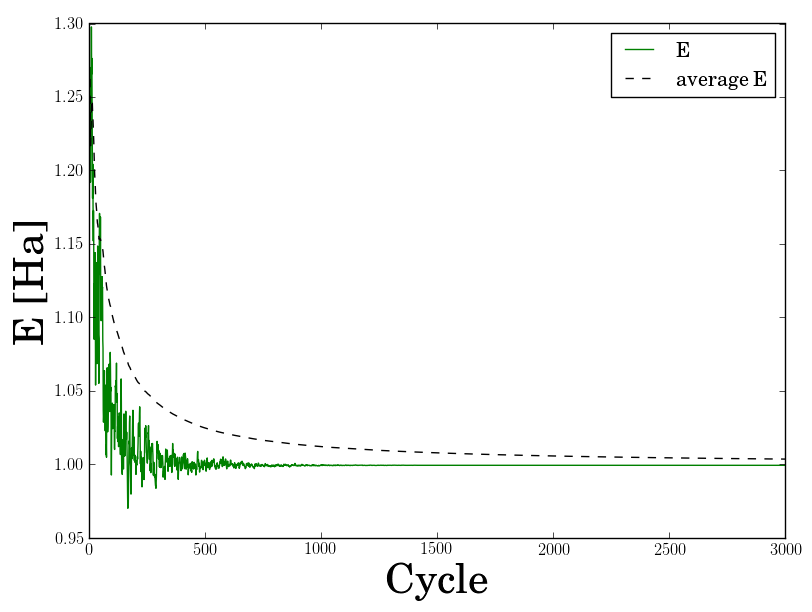
\includegraphics[scale=0.37]{../Graphics/ASGD_nonint_E.png}}
  \subfigure{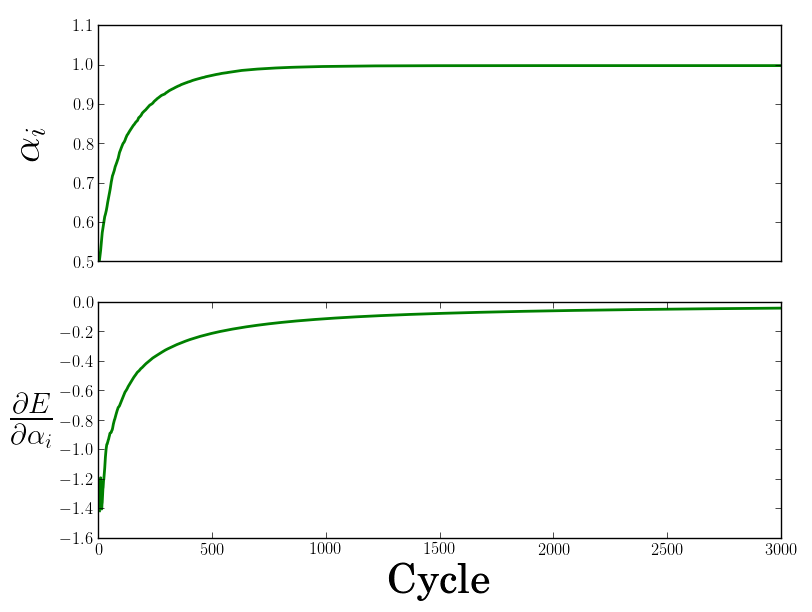
\includegraphics[scale=0.37]{../Graphics/ASGD_nonint.png}} 
  \caption{Adaptive Stochastic Gradient Descent (ASGD) results for a two-particle two-dimensional quantum dot with frequency $\omega=0.5$ and no electron-electron interaction. The exact energy $E_0=1$ is reached after approximately 1000 cycles, where the variational parameter $\alpha$ has converged close to unity. Due to enormous fluctuations the variational derivative is plotted as an accumulated average. The gradient is approximately zero after ~1000 cycles, in agreement with the behavior of the energy. The variational principle described in Section \ref{sec:selectingOptVarPar} is governing the trend of the energy convergence, however, a lot of statistical noise is present in the first 1000 cycles due to a high variance and a small number of samples.}
  \label{fig:ASGD_nonint}
 \end{center}
\end{figure}



\begin{figure}[h]
 \begin{center}
  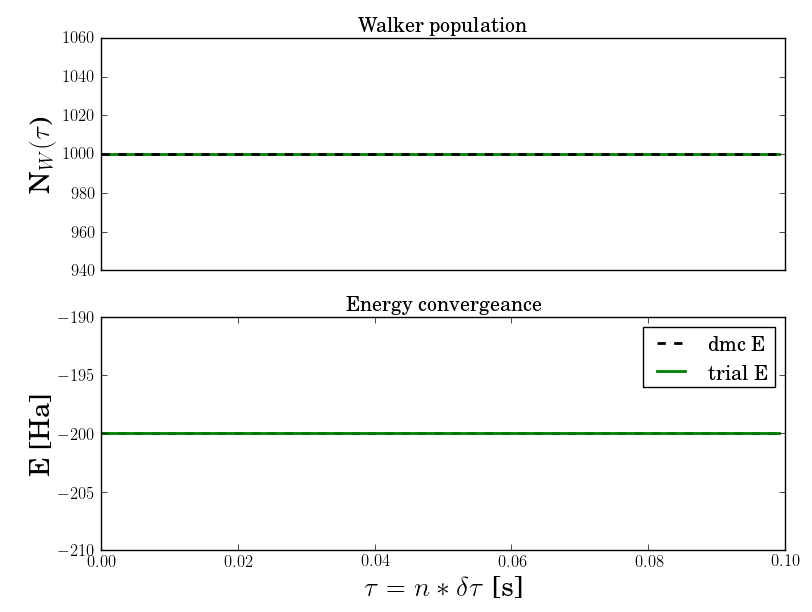
\includegraphics[scale=0.5]{../Graphics/DMC_neon_valid.png}
  \caption{Illustration of the Diffusion Monte-Carlo (DMC) energy convergence for the Neon atom listed in Table \ref{tab:res_valid_atoms}. The trial energy is fixed at the exact ground state energy as required. The number of walkers are constant, implying an approximately zero variance in the samples.}
  \label{fig:DMC_neon_nonint}
 \end{center}
\end{figure}

\begin{figure}[h]
 \begin{center}
  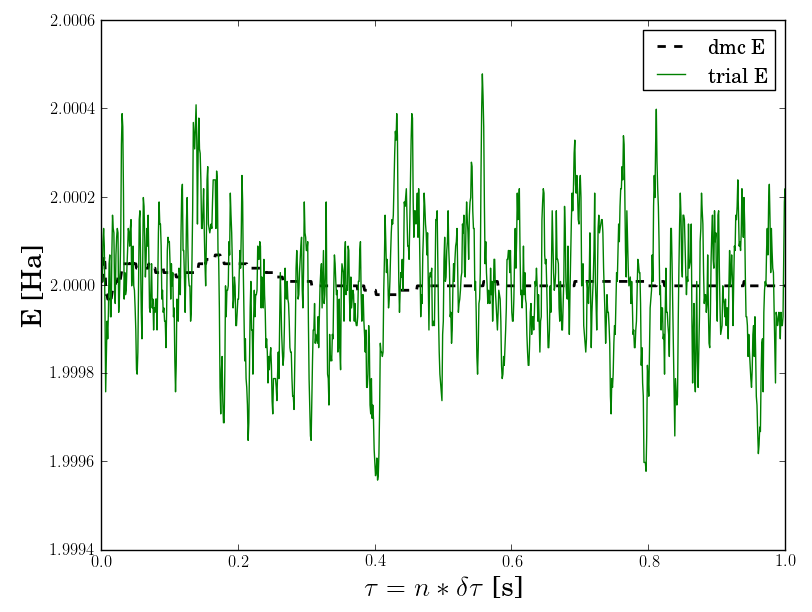
\includegraphics[scale=0.5]{../Graphics/DMC_notExactWF.png}
  \caption{Illustration of the Diffusion Monte-Carlo (DMC) energy convergence for a two-particle two-dimensional quantum dot with frequency $\omega=1$. The calculations are done with a variational parameter $\alpha=0.75$, where as the exact wave function is given for $\alpha=1$. Unlike the case with the exact wave function presented in figure \ref{fig:DMC_neon_nonint}, the trial energy oscillates around the exact value $E_0 = 2.0$. The final result reveals a DMC energy of $2.00000(2)$, where the original Variational Monte-Carlo (VMC) energy was $2.0042(3)$. This illustrates the power of DMC contra VMC in the interesting cases where the exact wave function is unknown. The calculation was done using $10000$ random walkers.}
  \label{fig:DMC_nonExactWF}
 \end{center}
\end{figure}
\clearpage
\section{Quantum Dots}

The focus regarding quantum dots has been on studying the distribution of electrons as a function of the level of confinement. In addition, ground state energies are provided and compared to other many-body methods to demonstrate the efficiency and precision of Variational Monte-Carlo (VMC) and Diffusion Monte-Carlo (DMC). In the case of two-dimensional quantum dots, there are multiple published results, however, for three dimensions this is not the case. An introduction to quantum dots is given in Section \ref{sec:modelQDots}. 

The double-well quantum dot has not been a focus in this thesis, however, some simple results are provided to demonstrate the flexibility of the code.

\subsection{Ground State Energies}

\subsubsection{Two-dimensional quantum dots}

Table \ref{tab:QDotsResultsAll} presents the calculated ground state energies for two-dimensional quantum dots in addition to corresponding results from methods such as Similarity Renormalization Group theory (SRG), Coupled Cluster Singles and Doubles (CCSD) and Full Configuration Interaction (FCI). In addition, some previously published DMC results are supplied. The references are listed in the table caption.

In light of the variational nature of DMC and VMC, the results show that DMC provides a more precise estimate for the ground state energy than VMC, both in terms of lower energies and lower errors. The exact energy in the case of two electrons with $\omega=1$ has been calculated in Ref. \cite{taut} and is $E_0 = 3$, which is in excellent agreement with the presented results.

The statistical errors in the DMC energies calculated in this thesis are lower than those provided in Ref. \cite{MagnusArticle}. This may only be due to the fact that the calculations in this thesis have been run on a super computer. Running smaller simulations on fewer processors result in larger errors. Both the implementations successfully agree with the FCI result for two particles, which strongly indicates that the disagreements in results are a result of systematic errors.    

In the case of two particles, DMC and FCI agree up to five decimals, which leads to the conclusion that DMC indeed is a very precise method. The SRG method is not variational in the sense that it can undershoot the exact energy. The DMC result should thus not be read as less precise in the cases where SRG provides a lower energy estimate. Diffusion Monte-Carlo and SRG are in excellent agreement for a large number of particles compared to FCI and CCSD, which drift away from the DMC results as their basis sizes shrink. 

For high frequencies, the VMC energy is higher than the CCSD energy. The fact that both the methods are variational implies that CCSD performs better than VMC in this frequency range. However, looking at the results the lower frequency range, it is clear that VMC performs better than CCSD. This is due to the fact that CCSD struggles with convergence as the correlations within the system increase, indicated by the decrease in number of shells used to perform the calculations.

The DMC energy is overall smaller than the CCSD energy, which, due to the variational nature of the methods, implies that DMC performs better than CCSD. Nevertheless, the results for $56$ particles are in excellent agreement. 

\setlength{\tabcolsep}{5pt}
\begin{table}
\begin{center}
\begin{tabular}{cc|rrrrrr}
    N     & $\omega$ & $\mathrm{E_{VMC}}$ & $\mathrm{E_{DMC}}$ & $E_\mathrm{ref}^{(a)}$& $E_\mathrm{ref}^{(b)}$ & $E_\mathrm{ref}^{(c)}$ & $E_\mathrm{ref}^{(d)}$\\
\hline\hline
\multicolumn{8}{c}{} \\
    2     &   0.01   & 0.07406(5)  & 0.073839(2)  & -		& -			& 0.0738 \{23\} & 0.07383505 \{19\}\\
          &   0.1    & 0.44130(5)  & 0.44079(1)   & - 		& - 			& 0.4408 \{23\} & 0.44079191 \{19\}\\
          &   0.28   & 1.02215(5)  & 1.02164(1)   & -		&0.99263 \{19\} 	& 1.0217 \{23\}  & 1.0216441 \{19\}\\
          &   0.5    & 1.66021(5)  & 1.65977(1)   & 1.65975(2)&1.643871 \{19\}	& 1.6599 \{23\}  & 1.6597723 \{19\}\\
          &   1.0    & 3.00030(5)  & 3.00000(1)   & 3.00000(3)&2.9902683 \{19\}	& 3.0002 \{23\}  & 3.0000001 \{19\}\\
\cline{2-8}
\multicolumn{8}{c}{} \\
    6     &   0.1    &  3.5690(3)  &  3.55385(5)  & -		&3.49991 \{18\} 	& 3.5805 \{22\}  & 3.551776 \{9\}\\
          &   0.28   &  7.6216(4)  &  7.60019(6)  & 7.6001(1) &7.56972 \{18\} 	& 7.6254 \{22\}  & 7.599579 \{6\}\\
          &   0.5    & 11.8103(4)  & 11.78484(6)  & 11.7888(2)&11.76228 \{18\}	& 11.8055 \{22\} & 11.785915 \{6\}\\
          &   1.0    & 20.1902(4)  & 20.15932(8)  & 20.1597(2)&20.14393 \{18\}	& 20.1734 \{22\} & 20.160472 \{8\}\\
\cline{2-8}
\multicolumn{8}{c}{} \\
    12    &   0.1    & 12.3162(5)  & 12.26984(8)  & - 		&12.2253 \{17\} 	& 12.3497 \{21\} & 12.850344 \{3\}\\
          &   0.28   & 25.7015(6)  & 25.63577(9)  & - 		&25.61084 \{17\} 	& 25.7095 \{21\} & 26.482570 \{2\}\\
          &   0.5    & 39.2343(6)  & 39.1596(1)   & 39.159(1) &39.13899 \{17\}	& 39.2194 \{21\} & 39.922693 \{2\}\\
          &   1.0    & 65.7905(7)  & 65.7001(1)   & 65.700(1) &65.68304 \{17\}	& 65.7399 \{21\} & 66.076116 \{3\}\\
\cline{2-8}
\multicolumn{8}{c}{} \\
    20    &   0.1    &  30.0729(8)  &  29.9779(1) & -		&29.95345 \{16\}	& 30.2700 \{8\} & 34.204867 \{1\}\\
          &   0.28   &  62.0543(8)  &  61.9268(1) & 61.922(2) &61.91368 \{16\}	& 62.0676 \{20\} & 67.767987 \{1\}\\
          &   0.5    &  94.0236(9)  &  93.8752(1) & 93.867(3) &93.86145 \{16\}	& 93.9889 \{20\} & 100.93607 \{1\}\\
          &   1.0    & 156.062(1)   & 155.8822(1) & 155.868(6)&155.8665 \{16\}	& 155.9569 \{20\}& 164.61280 \{1\}\\
\cline{2-8}
\multicolumn{8}{c}{} \\
    30    &   0.1    &  60.584(1)  &  60.4205(2)  & -		&60.43000 \{15\}	&  61.3827 \{9\}& -\\
          &   0.28   & 124.181(1)  & 123.9683(2)  & - 		&123.9733 \{15\}	& 124.2111 \{9\}& -\\
          &   0.5    & 187.294(1)  & 187.0426(2)  & - 		&187.0408 \{15\}	& 187.2231 \{19\}& -\\
          &   1.0    & 308.858(1)  & 308.5627(2)  & -	 	&308.5536 \{15\}	& 308.6810 \{19\}& -\\
\cline{2-8}
\multicolumn{8}{c}{} \\
    42    &   0.1    & 107.881(1)  & 107.6389(2)  & - 		&- 			& 111.7170 \{8\}& -\\
          &   0.28   & 220.161(1)  & 219.8426(2)  & - 		&219.8836 \{14\}	& 222.1401 \{8\}& -\\
          &   0.5    & 331.002(1)  & 330.6306(2)  & - 		&330.6485 \{14\}	& 331.8901 \{8\}& -\\
          &   1.0    & 544.2(8)    & 542.9428(8)  & - 		&542.9528 \{14\}	& 543.1155 \{18\}& -\\
\cline{2-8}
\multicolumn{8}{c}{} \\
    56    &   0.1    & 176.269(2) & 175.9553(7)   & -		& -		& 186.1034 \{9\} & -		\\
          &   0.28   & 358.594(2) & 358.145(2)    & -		& -		& 363.2048 \{9\} & -		\\
          &   0.5    & 538.5(6)   & 537.353(2)    & -		& -		& 540.3430 \{9\} & -		\\
          &   1      & 880.2(7)   & 879.3986(6)   & -		& -		& 879.6386 \{17\}& -		\\
\hline\hline


\end{tabular}
\caption{Ground state energy results for two-dimensional $N$-electron quantum dots with frequency $\omega$. Refs. $(a)$: F. Pederiva \cite{MagnusArticle} (DMC), $(b)$: S. Reimann \cite{Sarah} (Similarity Renormalization Group theory), $(c)$: C. Hirth \cite{Hirth} (Coupled Cluster Singles and Doubles), $(d)$: V. K. B. Olsen \cite{Olsen} (Full Configuration Interaction). The numbers inside curly brackets denote the number of shells used above the last filled shell, i.e.~above the so-called \textit{Fermi-level} \cite{Shavitt}, to construct the basis for the corresponding methods.}
\label{tab:QDotsResultsAll}
\end{center}
\end{table}
\setlength{\tabcolsep}{6pt}


\clearpage
\subsubsection{Three-dimensional quantum dots}

\setlength{\tabcolsep}{1.05cm}
\begin{table}
\begin{center}
\begin{tabular}{cc|rrr}
    N     & $\omega$ & $\mathrm{E_{VMC}}$ & $\mathrm{E_{DMC}}$ & $E_\mathrm{ref}$\\
\hline\hline
\multicolumn{5}{c}{} \\
    2     &   0.01   & 0.07939(3)  & 0.079206(3) & -		\\
          &   0.1    & 0.50024(8)  & 0.499997(3) & 0.5        \\
          &   0.28   & 1.20173(5)  & 1.201725(2) & -		\\
          &   0.5    & 2.00005(2)  & 2.000000(2) & 2.0 \\
          &   1.0    & 3.73032(8)  & 3.730123(3) & - \\
\cline{2-5}
\multicolumn{5}{c}{} \\
    8     &   0.1    & 5.7130(6)   & 5.7028(1)   & - 		\\
          &   0.28   & 12.2040(8)  & 12.1927(1)  & -		\\
          &   0.5    & 18.9750(7)  & 18.9611(1)  & -\\
          &   1.0    & 32.6842(8)  & 32.6680(1)  & -\\
\cline{2-5}
\multicolumn{5}{c}{} \\
    20    &   0.1    & 27.316(2)   & 27.2717(2)   & - 		\\
          &   0.28   & 56.440(2)   & 56.3868(2)   & -		\\
          &   0.5    & 85.714(2)   & 85.6555(2)   & - \\
          &   1.0    & 142.951(2)  & 142.8875(2)  & -\\
\cline{2-5}
\multicolumn{5}{c}{} \\
\hline\hline
\end{tabular}
\caption{Ground state energy results for three-dimensional $N$-electron quantum dots with frequency $\omega$. The values in the fifth column is exact calculations taken from Ref. \cite{taut}. The VMC result is as expected always higher than the corresponding DMC result.}
\label{tab:QDotsResults3D}
\end{center}
\end{table}
\setlength{\tabcolsep}{6pt}

The results for three-dimensional quantum dots are presented in Table \ref{tab:QDotsResults3D}. Three-dimensional quantum dots do not have the same foothold in literature as the two-dimensional ones, hence no results are listed except for some exact solutions taken from Ref. \cite{taut}. 

As expected, DMC reproduces the exact results for two particles. Compared to the exact results for two dimensions, which was reproduced with five digit precision, the exact results are reproduced with six decimal precision for three dimensions. This strongly indicates that for two electrons, DMC behaves better for three dimensions than for two. For higher number of particles, however, the errors are of the same order of magnitude as for two dimensions, leading to the conclusion that DMC performs equally good in either dimension for quantum dots. 

\subsection{One-body Densities}

The one-body densities are calculated using the methods described in Section \ref{sec:OBD}.

Figure \ref{fig:OBD_DMC_QDOTS_w1} presents the one-body densities for two-dimensional quantum dots. It is clear that the distributions are following a clear trend: The densities in the left column, that is, the densities for $N=2$, 12, and 30 particles, are all similar in shape. The shape for the $N=2$ case can be seen as the top of the $N=12$ density, which in turn can be seen as the top of the $N=30$ density. A physical explanation to this is that the shapes are conserved due to the fact that they represent energetically favorable configurations. 

The same trend is present for the distributions in the right column, that is, the densities for $N=6$, 20, and 42 particles. Viewing the distributions as a sequence of images, from the lowest number of particles to the highest, it is apparent that the shape propagates very much like water ripples. It is remarkable how the solutions to the most complex of equations can come in the form of simple patterns found all around nature.


\clearpage
\captionsetup[subfloat]{labelformat=empty}
\begin{figure}
 \begin{center}
  \subfigure[$N=2$]{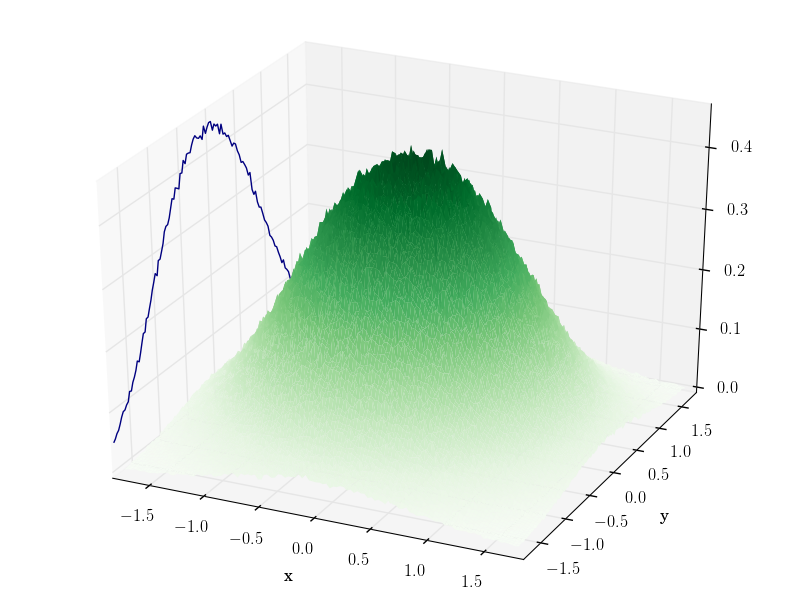
\includegraphics[scale=0.35]{../Graphics/OBD/OBD_DMC/dist_out_QDots2c1_3D.png}}
  \subfigure[$N=6$]{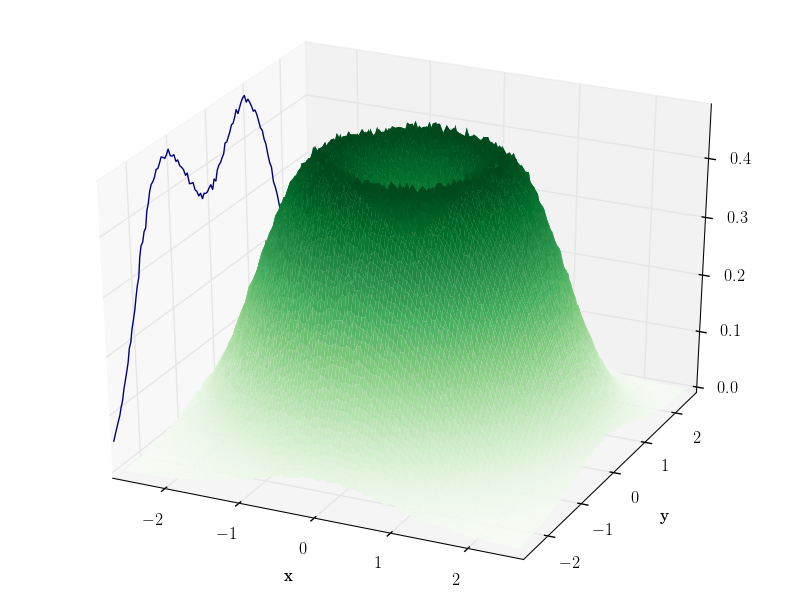
\includegraphics[scale=0.35]{../Graphics/OBD/OBD_DMC/dist_out_QDots6c1_3D.png}} \\
  \subfigure[$N=12$]{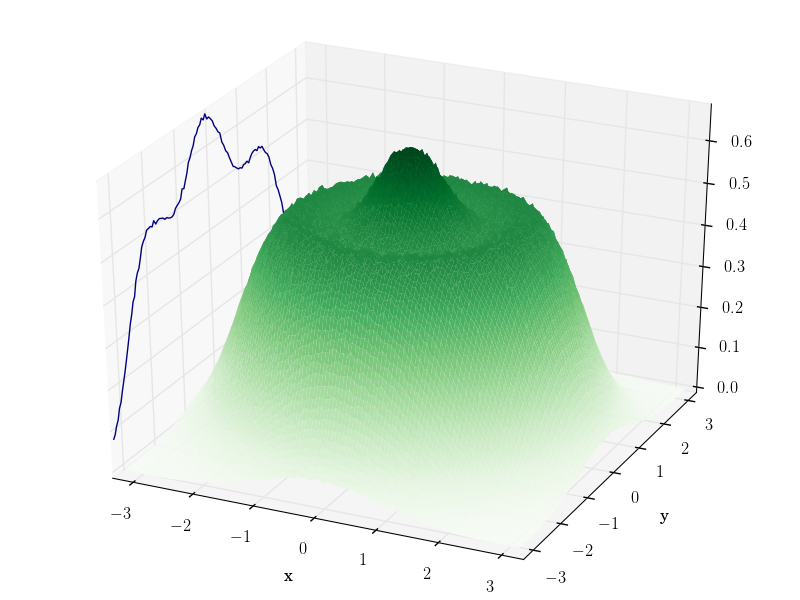
\includegraphics[scale=0.35]{../Graphics/OBD/OBD_DMC/dist_out_QDots12c1_3D.png}}
  \subfigure[$N=20$]{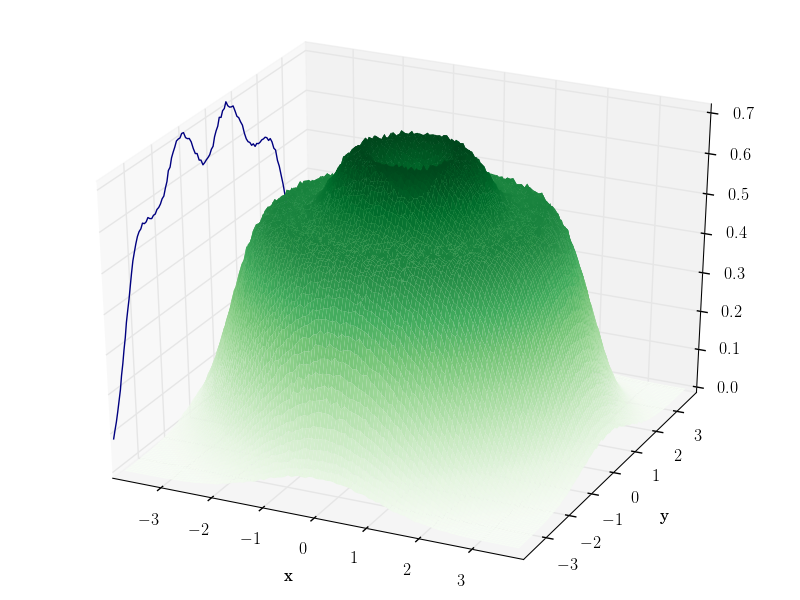
\includegraphics[scale=0.35]{../Graphics/OBD/OBD_DMC/dist_out_QDots20c1_3D.png}} \\
  \subfigure[$N=30$]{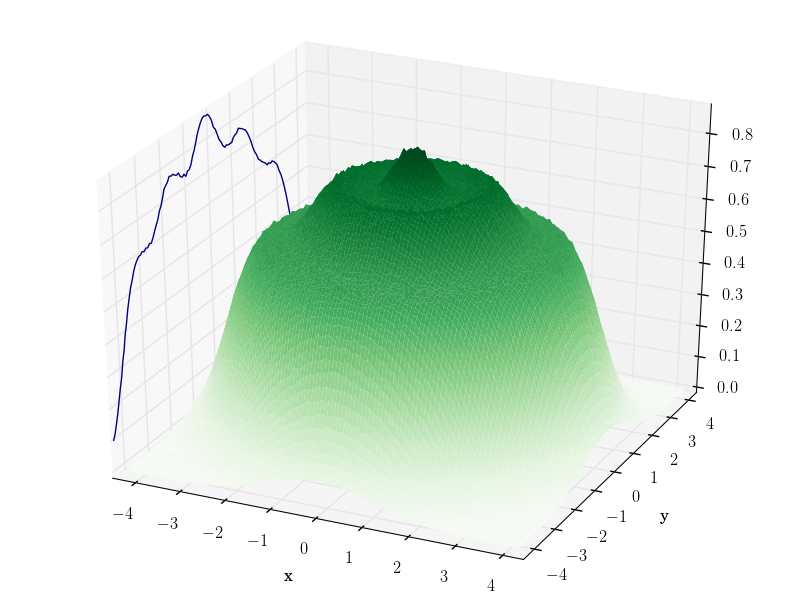
\includegraphics[scale=0.35]{../Graphics/OBD/OBD_DMC/dist_out_QDots30c1_3D.png}}
  \subfigure[$N=42$]{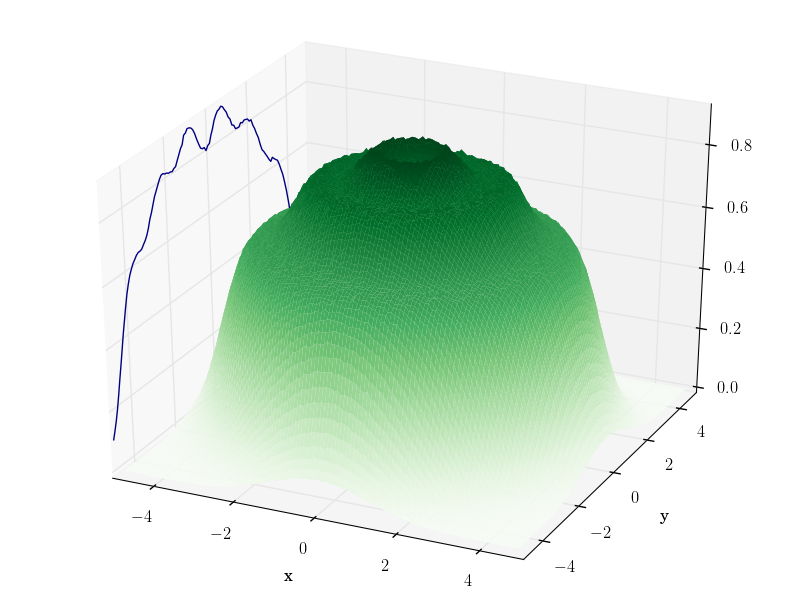
\includegraphics[scale=0.35]{../Graphics/OBD/OBD_DMC/dist_out_QDots42c1_3D.png}} \\
  \caption{Diffusion Monte-Carlo one-body densities for two-dimensional quantum dots with frequency $\omega=1$. The number of particles $N$ are listed below each density. It is apparent that the density behaves much like water ripples as the number of particles increase, conserving the shape in an oscillatory manner.}
  \label{fig:OBD_DMC_QDOTS_w1} 
 \end{center}
\end{figure}

\clearpage


Due to the electron-electron interaction, the Schrödinger equation is not separable in Cartesian coordinates. It is therefore not given that the insights from two dimensions can be transferred to the three-dimensional case. Nevertheless, by looking at the one-body densities for three dimensions in Figure \ref{fig:OBD_QDOTS3D_highfreq}, it is apparent that the general density profile is unchanged. The only thing separating two - and three-dimensional quantum dots is the number of electrons in the closed shells.

Note however, that this similarity only holds when the number of closed shells are equal. Comparing the two-dimensional density for $N=20$ electrons from Figure \ref{fig:OBD_DMC_QDOTS_w1} with the three-dimensional one for $N=20$ electrons given above, it is apparent that the shape of the densities are not conserved with respect to the number of particles $N$ alone.

% \setlength{\tabcolsep}{0.1pt}
\begin{figure}
 \begin{center}
 \begin{tabular}{cc|c}
   \subfigure{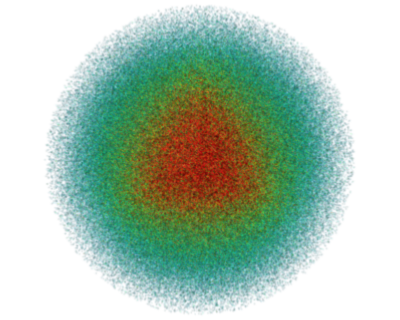
\includegraphics[scale=0.3]{../Graphics/OBD/OBD_Q3D/QD2w1_3D.png}} &
   \subfigure{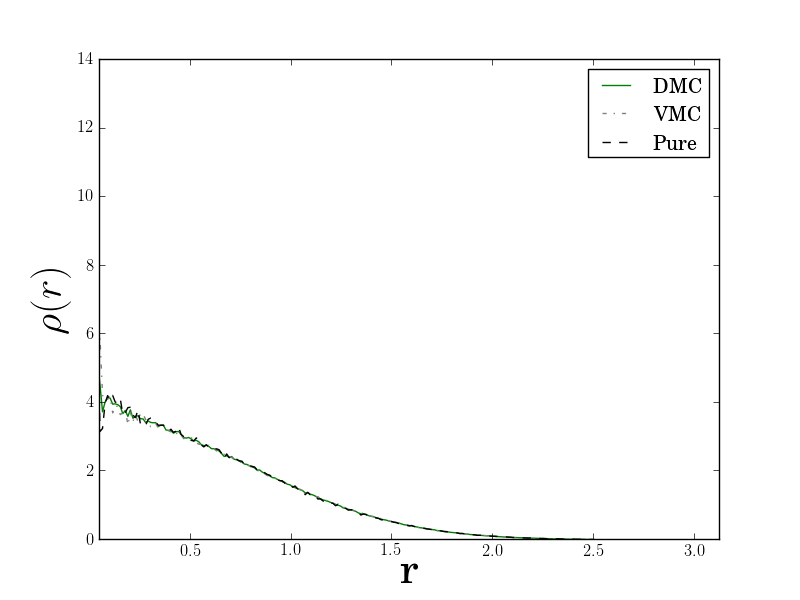
\includegraphics[scale=0.25]{../Graphics/OBD/OBD_Q3D/QD2w1_2D.png}} &
   \subfigure{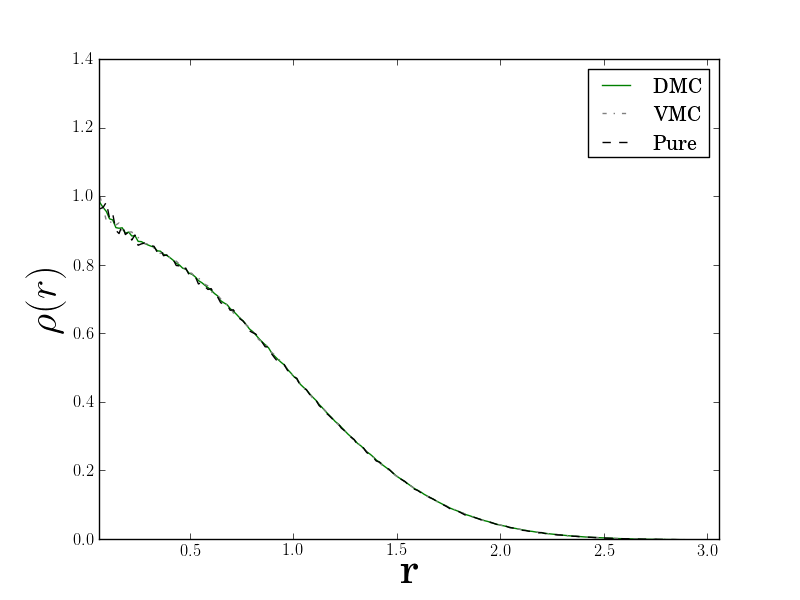
\includegraphics[scale=0.25]{../Graphics/OBD/OBD_Q3D/comp/Q2D_2.png}} \\
   \subfigure{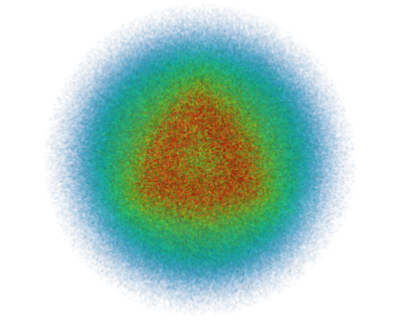
\includegraphics[scale=0.3]{../Graphics/OBD/OBD_Q3D/QD8w1_3D.png}} &
   \subfigure{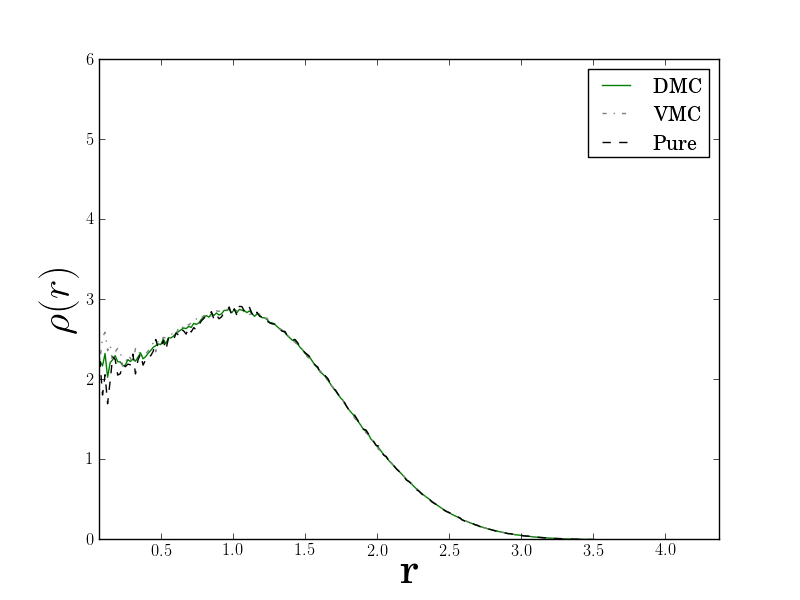
\includegraphics[scale=0.25]{../Graphics/OBD/OBD_Q3D/QD8w1_2D.png}} & 
   \subfigure{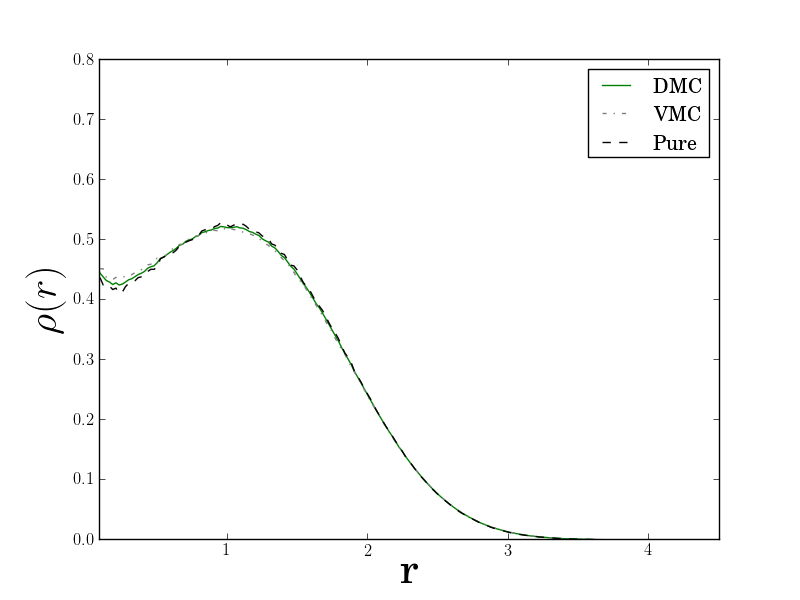
\includegraphics[scale=0.25]{../Graphics/OBD/OBD_Q3D/comp/Q2D_6.png}} \\
   \subfigure{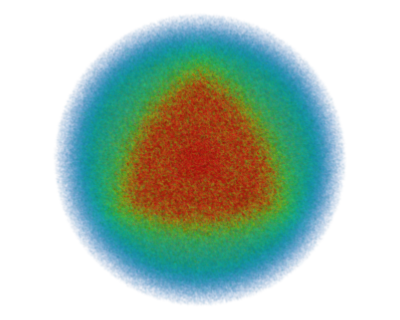
\includegraphics[scale=0.3]{../Graphics/OBD/OBD_Q3D/QD20w1_3D.png}} &
   \subfigure{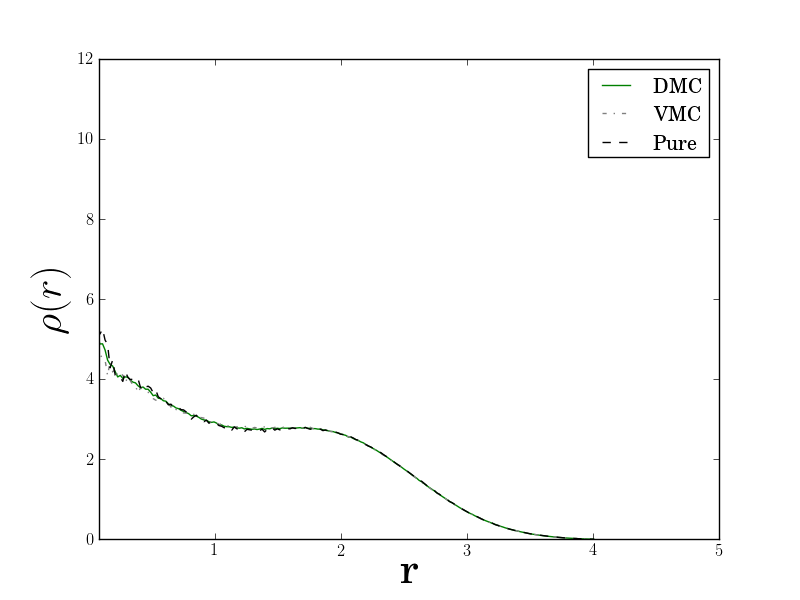
\includegraphics[scale=0.25]{../Graphics/OBD/OBD_Q3D/QD20w1_2D.png}} & 
   \subfigure{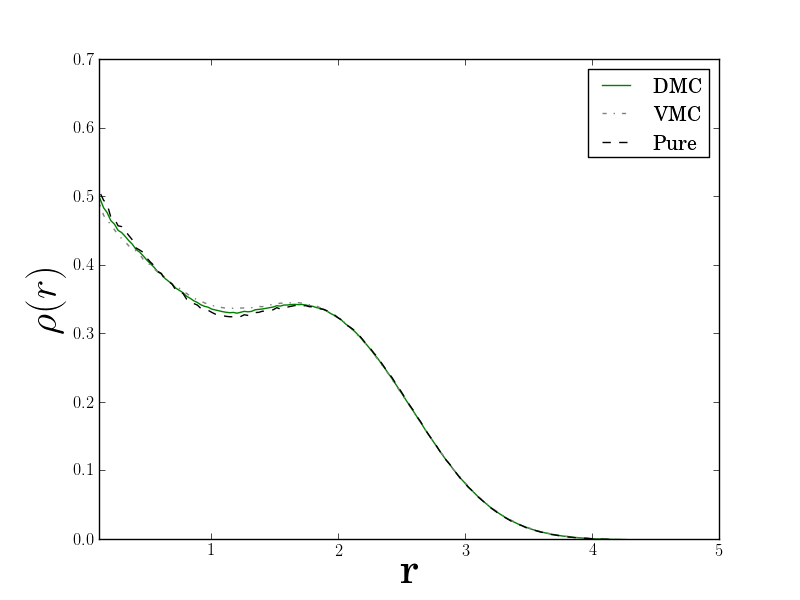
\includegraphics[scale=0.25]{../Graphics/OBD/OBD_Q3D/comp/Q2D_12.png}} \\
  \end{tabular}
  \caption{Left and middle column: One-body densities for quantum dots in three dimensions with frequency $\omega=1$. A quarter of the spherical density is removed to present a better view of the core.  Red and blue color indicate a low and high electron density, respectively. From top to bottom, the number of particles are $2$, $8$ and $20$. Right column: One-body densities for two-dimensional quantum dots for $N=2$, $6$ and $12$ electrons (from the top) with $\omega=1$. It is apparent that the  shape of the density is conserved as the third dimension is added. The radial densities are not normalized. Normalizing the densities would only change the vertical extent.}
  \label{fig:OBD_QDOTS3D_highfreq}
 \end{center}
\end{figure}
% \setlength{\tabcolsep}{pt}

\captionsetup[subfloat]{labelformat=parens}

\clearpage

\subsection{Lowering the frequency}

An interesting effect of lowering the frequency is that the two - and three-dimensional densities no longer match. For example, the radial density for the three-dimensional $N=8$ quantum dot from Figure \ref{fig:OBD_QDOTS3D_highfreq} was a near perfect match to the two-dimensional one for $N=6$ electrons, however, comparing the same densities for $\omega=0.01$ from Figures \ref{fig:OBD_QDOTS3D_lowfreq} and \ref{fig:OBD_DMC_QDOTS_lowering3D}, it is apparent that this is no longer the case; the two-dimensional density has a peak in the center region, whereas the three-dimensional density is zero in the center region.

From Figure \ref{fig:OBD_QDOTS3D_lowfreq} it is apparent that lowering the frequency increases the radial extent of the quantum dot, and thus lowers the electron density. Moreover, Figure \ref{fig:OBD_DMC_QDOTS_lowering3D} reveals that the electron density becomes similar in height and more localized across the quantum dot, which implies that the electrons on average are spread evenly in shell structures. The localization of the electrons is further verified in Figure \ref{fig:E_dist_qdots}, where is is clear that the expectation value of the total potential energy becomes larger than the corresponding kinetic energy.

In order words, an evenly spread and localized electron density gives rise to \textit{crystallization}\footnote{Unless at least one particle is frozen in the QMC simulations, the quantum dot densities should always be rotationally symmetric. Crystallization in a QMC perspective comes thus not in the form of actual ``crystals'', but rather as a rotated crystallized state.}. The idea of an electron crystal was originally proposed by Wigner \cite{WignerCrystalOrig}, hence the currently discussed phenomenon is referred to as a \textit{Wigner molecule} or a \textit{Wigner crystal}, which is expected for quantum dots in the limit of low electron densities where the total potential energy dominates over the kinetic energy \cite{WignerTransport, WignerPathTo, WignerSymmetryBreak, WignerFloating, Wigner2DQD}. These electronic crystals have been observed in experiments with for example liquid helium \cite{WignerExptHelium} and semiconductors \cite{WignerExptSemicond}.

\newcommand{\qqq}{\qquad\qquad\qquad}
\newcommand{\qq}{\qquad\qquad}
\newcommand{\rot}[1]{\begin{sideways}#1\end{sideways}}
\setlength{\tabcolsep}{0.1pt}
\begin{figure}
 \begin{center}
 \begin{tabular}{rl}
   \rot{$\qq\quad\omega=1$}&\subfigure{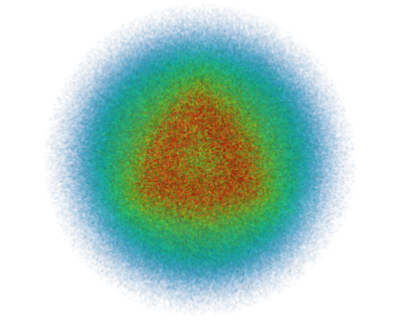
\includegraphics[scale=0.35]{../Graphics/OBD/OBD_Q3D/QD8w1_3D.png}}
   \subfigure{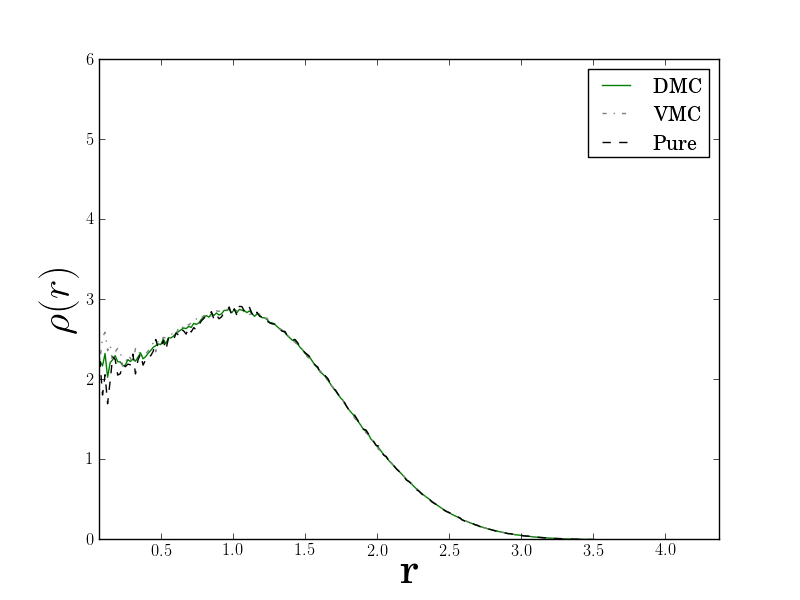
\includegraphics[scale=0.28]{../Graphics/OBD/OBD_Q3D/QD8w1_2D.png}} \\
   \rot{$\qq\omega=0.01$} &\subfigure{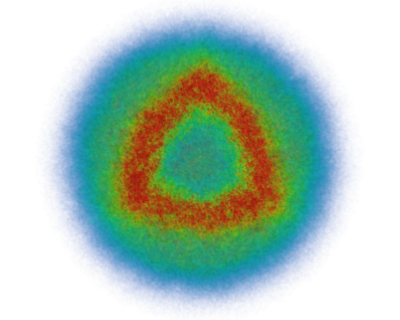
\includegraphics[scale=0.35]{../Graphics/OBD/OBD_Q3D/QD8w001_3D.png}} 
   \subfigure{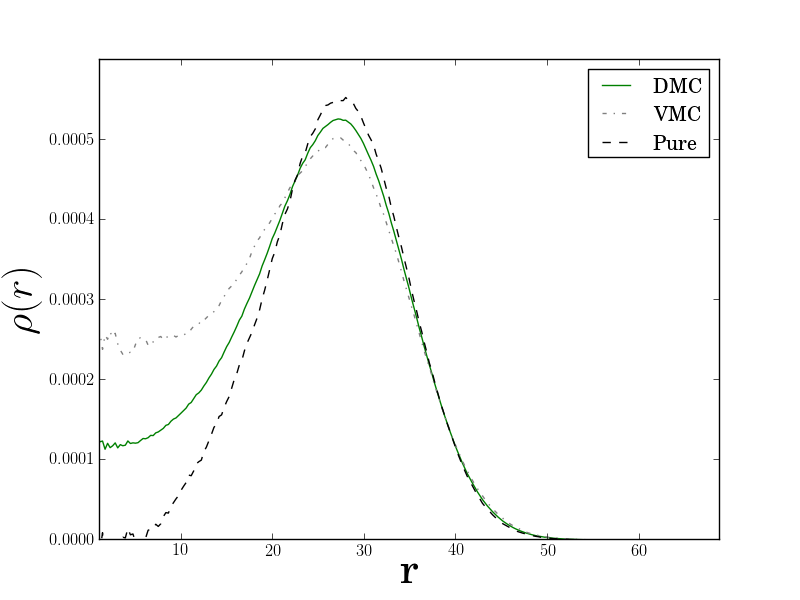
\includegraphics[scale=0.28]{../Graphics/OBD/OBD_Q3D/QD8w001_2D.png}}  \\
  \end{tabular}
  \caption{Comparison of the one-body densities for quantum dots in three dimensions for $N=8$ electrons for high and low frequency $\omega$. It is apparent that the distribution becomes more narrow as the frequency is reduced. Red and blue color indicate a low and high electron density, respectively. A quarter of the spherical density is removed to present a better view of the core. }
  \label{fig:OBD_QDOTS3D_lowfreq}
 \end{center}
\end{figure}

\captionsetup[subfloat]{labelformat=empty}
\newcommand{\OBDscale}{0.25}
\begin{landscape}
 \begin{figure}
 \begin{center}
 \begin{tabular}{rl}
  \rot{$\qquad\quad\omega=0.28$}&\subfigure{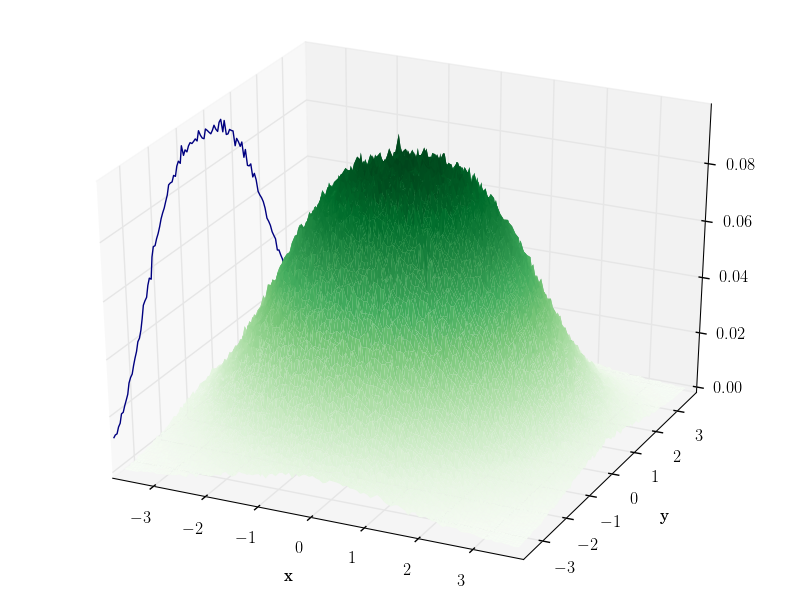
\includegraphics[scale=\OBDscale]{../Graphics/OBD/OBD_DMC/dist_out_QDots2c028_3D.png}}
  \subfigure{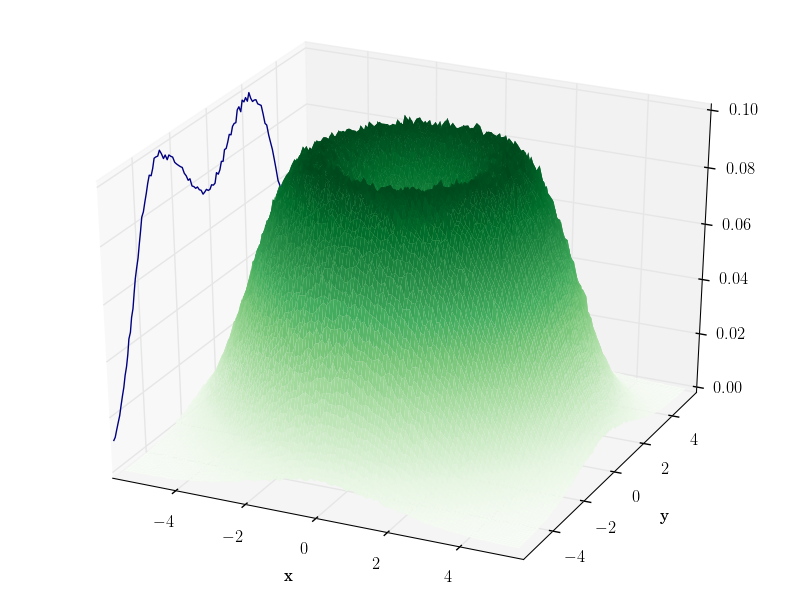
\includegraphics[scale=\OBDscale]{../Graphics/OBD/OBD_DMC/dist_out_QDots6c028_3D.png}} 
  \subfigure{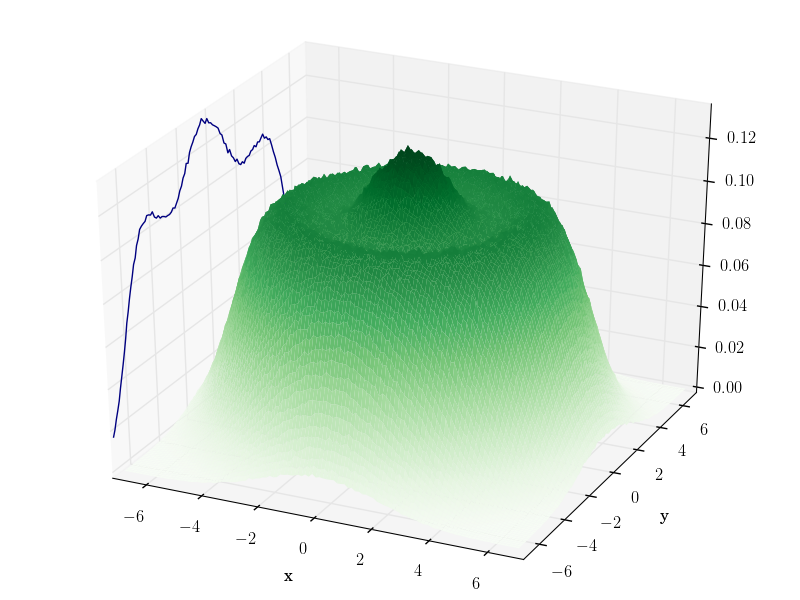
\includegraphics[scale=\OBDscale]{../Graphics/OBD/OBD_DMC/dist_out_QDots12c028_3D.png}}
  \subfigure{\includegraphics[scale=\OBDscale]{../Graphics/OBD/OBD_DMC/dist_out_QDots20c028_3D.png}} \\[-0pt]
  \rot{$\qquad\quad\omega=0.1$}&\subfigure{\includegraphics[scale=\OBDscale]{../Graphics/OBD/OBD_DMC/dist_out_QDots2c01_3D.png}}
  \subfigure{\includegraphics[scale=\OBDscale]{../Graphics/OBD/OBD_DMC/dist_out_QDots6c01_3D.png}} 
  \subfigure{\includegraphics[scale=\OBDscale]{../Graphics/OBD/OBD_DMC/dist_out_QDots12c01_3D.png}}
  \subfigure{\includegraphics[scale=\OBDscale]{../Graphics/OBD/OBD_DMC/dist_out_QDots20c01_3D.png}} \\[-0pt]
  \rot{$\qquad\quad\omega=0.01$}&\subfigure[$N=2$]{\includegraphics[scale=\OBDscale]{../Graphics/OBD/OBD_DMC/dist_out_QDots2c001_3D.png}}
  \subfigure[$N=6$]{\includegraphics[scale=\OBDscale]{../Graphics/OBD/OBD_DMC/dist_out_QDots6c001_3D.png}} 
  \subfigure[$N=12$]{\includegraphics[scale=\OBDscale]{../Graphics/OBD/OBD_DMC/dist_out_QDots12c001_3D.png}}
  \subfigure[$N=20$]{\includegraphics[scale=\OBDscale]{../Graphics/OBD/OBD_DMC/dist_out_QDots20c001_3D.png}} \\
 \end{tabular}
  \caption{\small{DMC One-body densities for Quantum Dots for decreasing oscillator frequencies $\omega$ and increasing number of particles $N$. Each row represents a given $\omega$, and each column represents a given $N$. Notice that the densities for $\omega=1$ (from Figure \ref{fig:OBD_DMC_QDOTS_w1}) are indistinguishable from those of $\omega=0.28$ except for their radial extent. This trend has been verified in the case of $N=30$, 42 and 56 electrons as well as for $\omega=0.5$, however, for the sake of transparency, these results are left out of the current figure.}}
  \label{fig:OBD_DMC_QDOTS_lowering3D}
 \end{center}
\end{figure}
\end{landscape}

\captionsetup[subfloat]{labelformat=parens}
\setlength{\tabcolsep}{6pt}


\captionsetup[subfloat]{labelformat=empty}
\begin{figure}[h]
 \begin{center}
  \subfigure[$N=6$]{\includegraphics[scale=0.35]{../Graphics/VirialPlots/E_vs_w_E6.png}}
  \subfigure[$N=42$]{\includegraphics[scale=0.35]{../Graphics/VirialPlots/E_vs_w_E42.png}} \\
  \caption{The relative magnitude of the expectation value of the different energy sources as a function of the frequency $\omega$ (left) together with the magnitude of the sources' energy contributions scaled with the oscillator frequency (right). The plots are supplied with legends to increase the readability. The different energy sources are the kinetic energy denoted \textit{Ekin}, the oscillator potential energy denonted \textit{Eosc}, and the electron-electron interaction energy denoted \textit{Ecol}. Note that all given energies are expectation values. The values are calculated using two-dimensional quantum dots. The number of electrons $N$ is displayed beneath each respective plot. It is apparent that the kinetic energy contribution is constant in both cases. Moreover, the oscillator potential contribution is more or less constant for the relative energies (left sub-figures). The figure clearly indicates that the potential energy contributions from the oscillator and the electron-electron interaction 
tends to dominate over the kinetic energy at lower frequencies.}
  \label{fig:E_dist_qdots}
 \end{center}
\end{figure}

It is expected that the QMC Wigner crystal corresponds to the electrons localizing around the equilibrium positions of the classical Wigner crystal\cite{WignerTransport}. Comparing the densities for two-dimensional quantum dots at $\omega=0.01$ for $N=6$, $12$, and $20$ electrons given in Figure \ref{fig:OBD_DMC_QDOTS_lowering3D} to similar classical calculations done in Ref. \cite{WignerClassic} for $N=6$, $10$, and $19$ electrons, respectively, it is apparent that the solutions match very well.  

It was mentioned previously that the Wigner crystallization of quantum dots came as a consequence of the average total potential energy being larger than the corresponding kinetic energy. This relationship between kinetic - and potential energy is closely related to the \textit{virial theorem} from classical mechanics. The quantum mechanical version of the virial theorem was proven by Fock in 1930 \cite{FockVirial} and reads

\begin{equation}
 V(\mathbf{r}) \propto r^\gamma \quad\longrightarrow\quad \langle \OP{T} \rangle = \frac{\gamma}{2} \langle \OP{V} \rangle, \label{eq:virial}
\end{equation}

where $\OP{T}$ and $\OP{V}$ denote the kinetic - and total potential energy operators, respectively. The important conclusion which can be drawn from this is that if two systems have an equal ratio of kinetic - to total potential energy, the systems behave identically in the sense that they follow the same effective potential, and thus have similar eigenstates. 

From Figure \ref{fig:V_dist_qdots} it is apparent that there is a remarkably constant slope for two different regions in the case of quantum dots, namely high - and low kinetic energy, which by looking at Figure \ref{fig:E_dist_qdots} corresponds to high - and low frequencies. In light of previous discussions, one may suggest that the change in the slopes
of Figure \ref{fig:V_dist_qdots} corresponds to the quantum dot system  making a transition into a Wigner crystallized state.



\newpage

\begin{figure}[h]
 \begin{center}
  \subfigure[$N=6$]{\includegraphics[scale=0.35]{../Graphics/VirialPlots/E_vs_w_V6.png}}
  \subfigure[$N=42$]{\includegraphics[scale=0.35]{../Graphics/VirialPlots/E_vs_w_V42.png}} \\
  \caption{The total kinetic energy vs. the total potential energy of two-dimensional quantum dots. The number of electrons $N$ are displayed beneath each respective plot. The axes are scaled with a power of $N$ to collapse the data to the same axis span. Once the kinetic energy drops below a certain energy dependent on the number of particles, the slope changes, which in light of the virial theorem from Eq.~(\ref{eq:virial}) indicates that the overall system changes properties. The data is fitted to linear lines with resulting slopes $a$ displayed in the legend. The parameter $r2$ indicates how well the data fits a linear line. An exact fit yields $r2 = 1$.}
  \label{fig:V_dist_qdots}
 \end{center}
\end{figure}
\captionsetup[subfloat]{labelformat=parens}

\subsection{Simulating a Double-well}

\begin{figure}[h]
 \begin{center}
 \includegraphics[scale=0.35]{../Graphics/DoubleWell.png}
  \caption{A countour plot of the trial wave function for a two-particle double-well quantum dot with the wells separated at a distance $R = 2$ in the $x$-direction using $m^\ast = \omega_0 = 1$. See Section \ref{sec:modelQDots} for an introduction to the double well potential. It is apparent that there is one electron located in each well, however, with a slight overlap in the middle region.}
  \label{fig:doubleWell}
 \end{center}
\end{figure}
\captionsetup[subfloat]{labelformat=parens}

Figure \ref{fig:doubleWell} shows the distribution for a two-particle simulation. It is apparent that despite the wells being separated, their local distributions overlap, indicating that the electrons can \textit{tunnel}, that is, they have a non-zero probability of appearing on the other side of the barrier. Comparing the distribution to the potential in Figure \ref{fig:extPotDoubleWell}, it is clear that they match very well.

The DMC result is $\mathrm{E_{DMC}} = 2.3496(1)$, whereas the non-interacting energy is $E_0 = 2$ and the single-well energy is $E_0=3.0$. It is expected that the energy lands in between these, as $R=0$ corresponds to the single well and $R\to\infty$ corresponds to the non-interacting case. 

\clearpage
\section{Atoms}
 
 The focus regarding atoms has been on simulating heavy atoms using a simple ansatz for the trial wave function, and thus test its limits. Due to the importance of atoms in nature, precise calculations which are believed to be very close to the exact result for the given Hamiltonian are done. These results will be featured as experimental results in the following discussions. For heavier atoms, relativistic effects become important due to the high energies of the valance electrons. Hence atoms heavier than krypton have not been studied. The specifics regarding the model used for atoms are given in Section \ref{sec:modelAtoms}.
 
\subsection{Ground State Energies}
 
 Table \ref{tab:AtomsRes} presents the ground state energy results for different atoms together with the experimental results. As expected, helium has the best match with the corresponding experimental result out of all the atoms. The relative precision of the heavier atoms are in the range $10^{-3}$ - $10^{-4}$, indicating that DMC performs equally well in all cases. However, the error in the calculations increases as the atoms become heavier. The calculations were done on a single node; running the calculations on several nodes with an increased number of walkers could reduce the errors somewhat. 
 
 In comparison to quantum dots, where the VMC and DMC results were relatively similar, it is evident that VMC performs rather poorly compared to DMC for atoms. Unlike quantum dots, the atomic systems allow for unbound states. This implies that the atomic systems in this thesis have an additional approximation in the trial wave function due to the fact that all the orbitals represent bound states. Nevertheless, this only further demonstrate the strengths of DMC to predict accurate results without much knowledge of the system at hand.
 
\begin{table}
\begin{center}
\begin{tabular}{lp{2cm}cclc}
Atom & & $E_\mathrm{VMC}$ & \qquad $E_\mathrm{DMC}$ & \qquad\,\, Expt. & \qquad $\epsilon_\mathrm{rel}$\\
\hline\hline
\ \\
He & \qquad & -2.8903(2) & \qquad -2.9036(2) & \qquad $-2.9037$ & \qquad $3.44\cdot 10^{-5}$\\
\ \\
Be & \qquad & -14.145(2) & \qquad -14.657(2)  & \qquad $-14.6674$ & \qquad $7.10\cdot 10^{-4}$ \\
\ \\
Ne & \qquad & -127.853(2) & \qquad -128.765(4) & \qquad $-128.9383$ & \qquad $1.34\cdot 10^{-3}$  \\
\ \\
Mg & \qquad & -197.269(3) & \qquad -199.904(8) & \qquad $-200.054$ & \qquad $7.50\cdot 10^{-4}$  \\
\ \\
Ar & \qquad & -524.16(7) & \qquad -527.30(4) & \qquad $-527.544$ & \qquad $4.63\cdot 10^{-4}$  \\
\ \\
Kr & \qquad & -2700(5) & \qquad -2749.9(2) & \qquad $-2752.054976$ & \qquad $7.83\cdot 10^{-4}$  \\
\ \\
\end{tabular}
\caption{Ground state energies for Atoms calculated using Variational - and Diffusion Monte-Carlo. Experimental energies are listed in the last column. As we see, DMC is rather close to the experimental energy. The relative error $\epsilon_\mathrm{rel} = |E_\mathrm{DMC} - \mathrm{Expt.}|/|\mathrm{Expt.}|$ is as expected lowest in the case of helium. The experimental energies, that is, the best possible results available, are taken from Ref. \cite{AtomsExact} for He through Ar, and \cite{KryptonExact} for Kr. }
\label{tab:AtomsRes}
\end{center}
\end{table}
 
 
 \subsection{One-body densities}
 
 The one-body densities for the \textit{noble gases}, that is, the closed shell atoms, are presented in Figure \ref{fig:OBD_noble_Atoms_2D_combo}. Comparing these to the one-body densities for the alkaline earth metals, i.e.~$\mathrm{Be}$, $\mathrm{Mg}$, etc., in Figure \ref{fig:OBD_alkaline_Atoms_2D_combo}, it is clear that the noble gases have a more confined electron distribution. This corresponds well to the fact that noble gases do not form compound materials, i.e.~molecules \cite{UniversityPhysics}. The alkaline earth metals, on the other hand, are found naturally as parts of compound materials. The one-body densities of the alkaline earth metals spreading out in space are thus in excellent agreement with what is expected.
 
It is apparent that the VMC distribution and the pure distribution differ more in the case of alkaline earth metals than for noble gases. This implies that the trial wave function is better in the case of noble gases. To explain this phenomenon, it is important to realize that for closed shell systems, which is the case of noble gases, the energy needed to excite an electron into the next $n$-shell is higher than the energy needed to excite an electron to the next $l$-level in an open shell system such as the alkaline earth metals. The result of this is that the contributions from the exited states to the total wave function in Eq.~(\ref{eq:MultiDeterminantTWF}) are higher for the alkaline earth metals than for the noble gases. This is exactly the same scenario as for high and low frequency quantum dots.

The approximation made in this thesis is that the trial wave function consists of a single determinant, thus neglecting the contribution from excited states. In light of the above discussion, this approximation is in other words better for noble gases than for the alkaline earth metals.
 
 
 
 \begin{figure}
 \begin{center}
   \subfigure{\includegraphics[scale=0.4]{../Graphics/OBD/OBD_Atoms/3D/Beryllium.png}} 
   \subfigure{\includegraphics[scale=0.3]{../Graphics/OBD/OBD_Atoms/2D/Beryllium.png}}  \\
   \subfigure{\includegraphics[scale=0.4]{../Graphics/OBD/OBD_Atoms/3D/Magnesium.png}} 
   \subfigure{\includegraphics[scale=0.3]{../Graphics/OBD/OBD_Atoms/2D/Magnesium.png}}  \\
  \caption{Three dimensional one-body densities (left column) and radial densities (right column) for alkaline earth metals; beryllium (top) and magnesium (bottom). A quarter of the spherical density is removed to present a better view of the core. Notice that the radial one-body densities in the right column are multiplied by the radius squared. This is done in order to reveal the characteristics behind a density which otherwise is a generic peak around the origin. Compared to the noble gases in Figure \ref{fig:OBD_noble_Atoms_2D_combo}, the alkaline earth metals have a surrounding dispersed probability cloud due to having easily excitable valence electrons. The element is thus more unstable and potent for chemical reactions and molecular formations through covalent - and ionic bonds \cite{UniversityPhysics}. Red and blue color indicate a low and high electron density, respectively.}
  \label{fig:OBD_alkaline_Atoms_2D_combo}
 \end{center}
\end{figure}
 
\begin{figure}
 \begin{center}
   \subfigure{\includegraphics[scale=0.4]{../Graphics/OBD/OBD_Atoms/3D/Helium.png}} 
   \subfigure{\includegraphics[scale=0.3]{../Graphics/OBD/OBD_Atoms/2D/Helium.png}}  \\
   \subfigure{\includegraphics[scale=0.4]{../Graphics/OBD/OBD_Atoms/3D/Neon.png}} 
   \subfigure{\includegraphics[scale=0.3]{../Graphics/OBD/OBD_Atoms/2D/Neon.png}}  \\
   \subfigure{\includegraphics[scale=0.4]{../Graphics/OBD/OBD_Atoms/3D/Argon.png}} 
   \subfigure{\includegraphics[scale=0.3]{../Graphics/OBD/OBD_Atoms/2D/Argon.png}}  \\
   \subfigure{\includegraphics[scale=0.4]{../Graphics/OBD/OBD_Atoms/3D/Krypton.png}} 
   \subfigure{\includegraphics[scale=0.3]{../Graphics/OBD/OBD_Atoms/2D/Krypton.png}}  \\
  \caption{One-body densities for noble gases. Counting top to bottom: Helium, neon, argon and krypton. A quarter of the spherical density is removed to present a better view of the core. Red and blue color indicate a low and high electron density, respectively. Notice that the radial one-body densities in the right column are multiplied by the radius squared. This is done in order to reveal the characteristics behind a density which otherwise is a generic peak around the origin.}
  \label{fig:OBD_noble_Atoms_2D_combo}
 \end{center}
\end{figure}
 
 

\clearpage
\section{Homonuclear Diatomic Molecules}

The focus regarding homonuclear diatomic molecules, from here on referred to as molecules, has been similar to the focus on atoms, with the exception of parameterizing atomic force fields which can be applied in molecular dynamics simulations. The implementation of molecular systems was achieved by adding $\sim 200$ lines of code. This fact by itself represents a successful result regarding the code structure. As for atoms, the optimal calculations are referred to as experimental results. Details regarding the transformation from atomic to molecular systems are given in Section \ref{sec:homoMolecules}.

\subsection{Ground State Energies}
 
\begin{table}
\begin{center}
\begin{tabular}{lrccrlrrc}
Molecule & $R$ & & \qquad & $E_\mathrm{VMC}$ & & \qquad $E_\mathrm{DMC}$ & \qquad\,\, Expt. & \qquad $\epsilon_\mathrm{rel}$\\
\hline\hline
\ \\
$\mathrm{H_2}$ & 1.4   & &\qquad & -1.1551(3)    & \qquad   & -1.1745(3)   & \qquad $-1.1746$      & \qquad $8.51\cdot 10^{-5}$ \\
\ \\
$\mathrm{Li_2}$& 5.051 & &\qquad & -14.743(3)    & \qquad   & -14.988(2)   & \qquad $-14.99544$    & \qquad $4.96\cdot 10^{-4}$ \\
\ \\
$\mathrm{Be_2}$& 4.63  & &\qquad & -28.666(5)    & \qquad   & -29.301(5)   & \qquad $-29.33854(5)$ & \qquad $1.28\cdot 10^{-3}$  \\
\ \\
$\mathrm{B_2}$ & 3.005 & &\qquad & -47.746(7)    & \qquad   & -49.155(5)   & \qquad $-49.4184$     & \qquad $5.33\cdot 10^{-3}$  \\
\ \\
$\mathrm{C_2}$ & 2.3481& &\qquad & -72.590(8)    & \qquad   & -74.95(1)    & \qquad $-75.923(5)$   & \qquad $1.28\cdot 10^{-2}$  \\
\ \\
$\mathrm{N_2}$ & 2.068 & &\qquad & -102.78(1)    & \qquad   & -106.05(2)   & \qquad $-109.5423$    & \qquad $3.19\cdot 10^{-2}$  \\
\ \\
$\mathrm{O_2}$ & 2.282 & &\qquad & -143.97(2)    & \qquad   & -148.53(2)   & \qquad $-150.3268$    & \qquad $1.2\cdot 10^{-2}$  \\
\ \\
\end{tabular}
\caption{Ground state energies for homonuclear diatomic molecules calculated using VMC and DMC. The distance between the atoms $R$ are taken from Ref. \cite{H_He_exact} for $\mathrm{H_2}$ and from Ref. \cite{UmrigarMolecules} for $\mathrm{Li_2}$ to $\mathrm{O_2}$. The experimental energies, that is, the best possible results available, are taken from Ref. \cite{H_He_exact} for $\mathrm{H_2}$ and from Ref. \cite{ExactMolecules} for $\mathrm{Li_2}$ to $\mathrm{O_2}$. As expected DMC is closer to the experimental energy than VMC. Moreover, the relative error $\epsilon_\mathrm{rel} = |E_\mathrm{DMC} - \mathrm{Expt.}|/|\mathrm{Expt.}|$ is as expected lowest in the case of $\mathrm{H_2}$, and increases with atomic number.}
\label{tab:MoleculesRes}
\end{center}
\end{table}

Table \ref{tab:MoleculesRes} lists the VMC and DMC results with the corresponding experimental energies for $\mathrm{H_2}$ through $\mathrm{O_2}$. As expected, the two-particle result is very close to the experimental value with the same precision as the result for the helium atom in Table \ref{tab:AtomsRes}. The relative error from the experimental energy increases with atomic number, and is far higher than the errors in the case of pure atoms. This comes as a result of the trial wave function being less optimal due to the fact that it does not account for the atomic nuclei interaction term in the molecular Hamiltonian. Nevertheless, taking the simple nature of the trial wave function into consideration, the calculated energies are satisfyingly close to the experimental ones. 

As with atoms, the energies were calculated on a single node, resulting in a rather big statistical error in DMC. Doing the calculations on a supercomputer with an increase in the number of walkers should decrease the errors.

\subsection{One-body densities}

Figure \ref{fig:OBD_Molecules} presents the one-body densities of $\mathrm{Li_2}$, $\mathrm{Be_2}$ and $\mathrm{O_2}$. The densities have strong peaks located at a distance equal to half of the listed core separation $R$, indicating that the atomic nuclei interaction still dominates the general shape of the distributions. Moreover, it is clear by looking at the figure that most of the electrons are on the side facing the opposite nucleus, leading to the conclusion that the molecules share a covalent bond \cite{UniversityPhysics}. This is especially clear in the case of the oxygen molecule, where there is a small formation of electrons on the inner side of the nuclei.

\vspace{2cm}
\renewcommand\floatpagefraction{.9}
\begin{figure}[h]
 \begin{center}
   \subfigure{\includegraphics[scale=0.4]{../Graphics/OBD/OBD_MOL/Li2_3D.png}} 
   \subfigure{\includegraphics[scale=0.3]{../Graphics/OBD/OBD_MOL/Li2_2D.png}}  \\
   \subfigure{\includegraphics[scale=0.4]{../Graphics/OBD/OBD_MOL/Be2_3D.png}} 
   \subfigure{\includegraphics[scale=0.3]{../Graphics/OBD/OBD_MOL/Be2_2D.png}}  \\
   \subfigure{\includegraphics[scale=0.4]{../Graphics/OBD/OBD_MOL/O2_3D.png}} 
   \subfigure{\includegraphics[scale=0.3]{../Graphics/OBD/OBD_MOL/O2_2D.png}}
  \caption{One-body densities of $\mathrm{Li_2}$ (top), $\mathrm{Be_2}$ (middle) and $\mathrm{O_2}$ (bottom). The figures to the left are spherical densities sliced through the middle to better reveal the core structure. The figures to the right are radial one-body densities projected on the nucleus-nucleus axis. Red and blue color indicate a high and low electron density, respectively. The right-hand figures are symmetric around the origin.}
  \label{fig:OBD_Molecules}
 \end{center}
\end{figure}
\renewcommand\floatpagefraction{.7}

\clearpage
\subsection{Parameterizing Force Fields}

\begin{figure}
 \begin{center}
  \subfigure[$\mathrm{H_2}$]{\includegraphics[scale=0.37]{../Graphics/R_VS_E/R_vs_E_hyd_pure.png}}
  \subfigure[$\mathrm{Li_2}$]{\includegraphics[scale=0.37]{../Graphics/R_VS_E/R_vs_E_lit_pure.png}} 
  \caption{Top figures: The distance between the atoms $R$ vs. the potential and total energy calculated using QMC. To the left: $\mathrm{H_2}$. To the right: $\mathrm{Li_2}$. It is evident that there exists a well-defined energy minimum in the case of hydrogen. For lithium this is not the case, which is expected since lithium does not appear naturally in a diatomic gas phase, but rather as an ionic compound in other molecules \cite{UniversityPhysics}. Bottom figure: The general shape of the Lennard-Jones potential commonly used in molecular dynamics simulations as an approximation to the potential between atoms. The top figures clearly resemble the Lennard-Jones 12-6 potential, leading to the conclusion that QMC calculations can be used to parameterize a more realistic potential.}
  \label{fig:molecules_R_vs_E}
  \setcounter{subfigure}{2}
  \subfigure[The Lennard-Jones 12-6 potential with $\sigma=\epsilon=1$.]{\includegraphics[scale=0.5]{../Graphics/R_VS_E/LD.png}}
  \label{fig:LennardJones}
 \end{center}
\end{figure}

In molecular dynamics, it is custom to use the \textit{Lennard Jones 12-6 potential} as an ansatz to the interaction between pairs of atoms \cite{MD1, MD2}

\begin{equation}
 V(R) = 4\epsilon \left(\left(\frac{\sigma}{R}\right)^{12} - \left(\frac{\sigma}{R}\right)^{6}\right),
\end{equation}

where $\epsilon$ and $\sigma$ are parameters which can be fit to a given system.

However, the force field can be parameterized in greater detail using QMC calculations, resulting in a more precise molecular dynamics simulation \cite{forcesQMC}. The quantity of interest is the \textit{force}, that is, the gradient of the potential. The classical potential in molecular dynamics does not correspond to the potential in the Schrödinger equation, due to the fact that the kinetic energy contribution from the electrons is not counted as part of the total kinetic energy in the molecular dynamics simulation. Hence it is the total energy of the Schrödinger equation which corresponds to the potential energy in molecular dynamics. In the case of diatomic molecules this means that 

\begin{equation}
 F_\mathrm{MD} = \frac{\mathrm{d}\langle E \rangle}{\mathrm{d}R}.
\end{equation}

Expressions for this derivative can be obtained in ab-initio methods by using the Hellmann-Feynman theorem \cite{forcesQMC}. However, the derivative can be approximated by the slope of the energy in Figure \ref{fig:molecules_R_vs_E}. The figure shows that there are clear similarities between the widely used Lennard-Jones 12-6 potential and the results of QMC calculations done in this thesis, leading to the conclusion that the current state of the code can in fact produce approximations to atomic force fields for use in molecular dynamics.

For more complicated molecules, modelling the force using a single parameter $R$ does not serve as a good approximation. However, the force can be found as a function of several angles, radii, etc., which in turn can be used to parameterize a more complicated molecular dynamics potential. An example of such a potential is the \textit{ReaxFF} potential for hydrocarbons \cite{ReaxFF}.






 
 

 
 
 





\clearpage
\appendix
%% \noappendixpagetoc
%% \noappendixheadtotoc
\appendixpage
\chapter{Dirac Notation}
\label{app:Dirac}

Calculations involving sums over inner products of orthogonal states are common in Quantum Mechanics. This due to the fact that eigenfunctions of Hermitian operators, which is the kind of operators which represent observables\cite{griffiths}, are necessarily orthogonal\cite{golub1996matrix}. These inner-products will in many cases result in either zero or one, i.e.~the \textit{Kronecker-delta} function $\delta_{ij}$; explicitly calculating the integrals is unnecessary. 

\textit{Dirac notation} is a notation in which quantum states are represented as abstract components of a \textit{Hilbert space}, i.e.~an inner product space. This implies that the inner-product between two states are represented by these states alone, without the integral over a specific basis, which makes derivations a lot cleaner and general in the sense that no specific basis is needed.

Extracting the abstract state from a wave function is done by realizing that the wave function can be written as the inner product between the position basis eigenstates $\ket{x}$ and the abstract quantum state $\ket{\psi}$ 

\begin{equation*}
 \psi(x) = \langle r, \psi \rangle \equiv \braket{x}{\psi} = \bra{x}\times\ket{\psi}. 
\end{equation*}


The notation is designed to be simple. The right hand side of the inner product is called a \textit{ket}, while the left hand side is called a \textit{bra}. Combining both of them leaves you with an inner product bracket, hence Dirac notation is commonly referred to as \textit{bra-ket} notation. 

To demonstrate the simplicity introduced with this notation, imagine a coupled two-level spin-$\frac{1}{2}$ system in the following state

\begin{eqnarray}
 \ket{\chi} &=& N\Big[\ket{\su\sd} -i\ket{\sd\su}\Big]\\
 \bra{\chi} &=& N\Big[\bra{\su\sd} +i\bra{\sd\su}\Big]
\end{eqnarray} 

Using the fact that both the $\ket{\chi}$ state and the two-level spin states should be orthonormal, the normalization factor can be calculated without explicitly setting up any integrals

\begin{eqnarray*}
 \braket{\chi}{\chi} &=& N^2\Big[\bra{\su\sd} +i\bra{\sd\su}\Big]\Big[\ket{\su\sd} -i\ket{\sd\su}\Big] \\
 &=& N^2\Big[\braket{\su\sd}{\su\sd} + i\braket{\sd\su}{\su\sd} - i\braket{\su\sd}{\sd\su} + \braket{\sd\su}{\sd\su}\Big] \\
 &=& N^2\Big[1 + 0 - 0 + 1\Big] \\
 &=& 2N^2\\
 &=& 1,
\end{eqnarray*}

This implies the trivial solution $N=1/\sqrt{2}$. With this powerful notation at hand, important properties such as the \textit{completeness relation} of a set of states can be shown. A standard strategy is to start by expanding one state $\ket{\phi}$ in a complete set of different states $\ket{\psi_i}$:

\begin{eqnarray*}
 \ket{\phi}            &=& \displaystyle\sum_i c_i\ket{\psi_i}\\
 \braket{\psi_k}{\phi} &=& \displaystyle\sum_i c_i\underbrace{\braket{\psi_k}{\psi_i}}_{\delta_{ik}}\\
                       &=& c_k\\
 \ket{\phi}            &=& \displaystyle\sum_i \braket{\psi_i}{\phi}\ket{\psi_i}\\
                       &=& \left[\displaystyle\sum_i \ket{\psi_i}\bra{\psi_i}\right]\ket{\phi} 
\end{eqnarray*}

which implies that

\begin{equation}
 \displaystyle\sum_i \ket{\psi_i}\bra{\psi_i} = \I
 \label{eq:Completeness}
\end{equation}

for any complete set of orthonormal states $\ket{\psi_i}$. Calculating the corresponding identity for a continuous basis like e.g.~the position basis yields

\begin{eqnarray}
 \int |\psi(x)|^2dx    &=& 1 \label{eq:posIdentityFirst} \\
 \int |\psi(x)|^2dx    &=& \int \psi^\ast(x)\psi(x)\mathrm{d}x \nonumber \\
                       &=& \int \braket{\psi}{x}\braket{x}{\psi}\mathrm{d}x \nonumber \\
                       &=& \bra{\psi}\Big[\int \ket{x}\bra{x}dx\Big]\ket{\psi} \label{eq:posIdentityLast}.
\end{eqnarray}

Combining eq.~\ref{eq:posIdentityFirst} and eq.~\ref{eq:posIdentityLast} with the fact that $\braket{\psi}{\psi} = 1$ yields the identity

\begin{equation}
 \int \ket{x}\bra{x}dx = \I.
 \label{eq:CompletenessCont}
\end{equation}

Looking back at the introductory example, this identity is exactly what is extracted when a wave function is described as an inner product instead of an explicit function.

\chapter{Visualization of Data}

With an increasingly massive code framework comes the increased need of data analysis tools. Data analysis usually involves visualization of the data; there is only so much information a single number can hold. To supplement the QMC code, a visualization tool has been developed, dramatically easing the implementation of additional visualization scripts.

\section{DCViz}

The tool DCViz (Dynamic Column data Visualizer) is a Python based visualization tool designed to plot data stored in columns. The plot library used is \textit{Matplotlib}. The data can be plotted dynamically at a specified interval, and is hence designed to run parallel to the main application, e.g. DMC. The convergence of the DMC method is much better represented by a trailing energy graph than simply a stream of numbers. The same goes for the minimization process.

\subsection{Implementing a Visualization Tool}

Just like for the \verb+orbitalsGenerator+ tool (see Appendix \ref{appendix:sympy}), specific implementations come in the shape of subclasses of the DCViz superclass. All the functionality regarding setting up figures, re-plotting dynamically, clearing figures to avoid random crashes if used repeatedly, etc. is inherited from the superclass. The necessary elements to implement is

\begin{small}
\begin{tabular}{lp{14cm}}
\verb+figMap+		& A dictionary representing the names and structure of the plotted figures. If e.g. two figures 				\verb+fig1+ and \verb+fig2+ are wanted, where \verb+fig1+ should contain three sub-figures 					\verb+subFig1+, \verb+subFig2+ and \verb+subFig3+, the figure map should be set up as \\					& \verb+figMap = {"fig1": ["subFig1", "subFig2", "subFig3"], "fig2": ["subFig4"]}+ \\
			& In class member functions, e.g. \verb+self.subFig1+ will be available as the figure representing the first sub-figure of the first figure. \\
			\ \\
\verb+nametag+		& A string representing the name of the output files associated with the given implementation 				(subclass). Full regular expressions support. E.g. \verb|nametag = "DMC_out_\d+\.dat"|. All files
			loaded which matches the name-tag will be automatically plotted by the corresponding subclass implementation. \\
			\ \\
\verb+plot(self, data)+& The loaded file will be loaded into a \verb+data+ object, which is an iterator where each elements
			represents a column in the data file. Designed such that expressions such as \verb+col1, col2 = data+ is possible (and fast). For the raw data loaded in a matrix, use \verb+data.data+ to directly access the loaded file.
			\ \\
			&In the plot function, the sub-figures introduced in \verb+figMap+ should be loaded with data through e.g. \verb+self.subFig1.plot(col1, col2)+. The superclass' main loop will take care of the rest.
\end{tabular}
\end{small}

An example implementation would be

\vspace{0.5cm}
\begin{lstlisting}[language=Python]
class myTestClass(DCVizPlotter):
    nametag =  'testcase\d\.dat' #filename with regex support
    
    #1 figure with 1 subfigure
    figMap = {'fig1': ['subfig1']}
    
    #skip first row.
    skipRows = 1    
    
    def plot(self, data):
        column1 = data[0]

        self.subfig1.set_title('I have $\LaTeX$ support!')
              
        self.subfig1.set_ylim([-1,1])
          
        self.subfig1.plot(column1)
\end{lstlisting}



\subsection{Additional Support}

Additional parameters can be overloaded for additional functionality

\begin{small}
\begin{tabular}{lp{14cm}}
\verb+nCols+ & The number of columns present in the file. Will be automatically detected unless the data is stored in binary format.\\
\verb+skipRows+ & The number of initial rows to skip. Will be automatically detected unless the data is stores as a single column.\\
\verb+skipCols+ & The number of initial columns to skip. Defaults to zero.\\
\verb+armaBin+ & Boolean flag. If set to true, the data is assumed to be stored in Armadillo's binary format (doubles). Number of columns and rows will be read from the file header.\\
\verb+fileBin+ & Boolean flag. If set to true, the data is assumed to be stores in binary format. The number of columns must be specified.
\end{tabular}
\end{small}

The \LaTeX support is enabled if the correct packages is installed.

\subsubsection{Families}

A specific implementation can be flagged to belong to a family by setting the class member variable \verb+isFamilyMember+ to true. If this flag is true, the folder where the originally data was loaded will be scanned for additional matches, all of which will be loaded into the \verb+data+ input to the plot function. In this case each element of the \verb+data+ list would be a column iterator as explained previously.

To keep track of which file a given data-set was loaded from, a list \verb+self.familyFileNames+ is created, where element $i$ is the filename corresponding to \verb+data[i]+.

A class member string \verb+familyName+ can be overridden to display a more general name in the auto-detection feedback. An example implementation using data file families would be
\vspace{0.5cm}
\begin{lstlisting}[language=Python]
class myTestClassFamily(DCVizPlotter):
    nametag =  'testcaseFamily\d\.dat' #filename with regex support
    
    #1 figure with 3 subfigures
    figMap = {'fig1': ['subfig1', 'subfig2', 'subfig3']}
    
    #skip first row of each data file.
    skipRows = 1    

    #Using this flag will read all the files matching the nametag
    #(in the same folder.) and make them aviable in the data arg    
    isFamilyMember = True
    familyName = "testcase"
    
    def plot(self, data):
        
        #figures[0] is 'fig1' figures. the 0'th element is the
        #self.fig1 itself. Subfigures are always index [1:]
        mainFig = self.figures[0][0]  
        mainFig.suptitle('I have $\LaTeX$ support!')        
        subfigs = self.figures[0][1:]
    
        #Notice we plot fileData.data (In order to get the numpy object) 
        #and not fileData alone, as fileData is a 'dataGenerator' instance 
        #used to speed up file reading. Alternatively, we could send data[:]
        for subfig, fileData in zip(subfigs, data):
            subfig.plot(fileData.data)
            subfig.set_ylim([-1,1])
\end{lstlisting}

loading e.g. \verb+testcaseFamily0.dat+ would automatically load \verb+testcaseFamily1.dat+ etc. as well.

\subsection{Usage: The API, Terminal Client and GUI}

All listed interfaces to the DCViz core has full warning support and reconfigurability. DCViz, like the QMC code in general, is designed to be used by other people than the Author.

\subsubsection{The Application Programming Interface (API)}
The DCViz library has been developed to interface nicely with any python script \footnote{DCViz can also be called through C++, however, no header has been implemented for this. Typically one would use the std::system or std::thread to start the script in the background.} Given a path to the data file, all that is needed in order to visualize it is


\begin{lstlisting}[language=Python]
import DCVizWrapper as viz
dynamicMode = False #or true

...
#Perform some calculations and store these in the file myDataFile (including path)

#DCVizWrapper.main() automatically detects the subclass implementation 
#matching the specified file. Thread safe and easily interruptable.
viz.main(path=myDataFile, dynamic=dynamicMode)
\end{lstlisting}

\subsubsection{Using the Terminal}

The \verb+DCVizWrapper.py+ script can also be called directly from a terminal using the path as first command line argument. If the option \verb+-d+ is supplied, dynamic mode is activated.

\subsubsection{The GUI}

The script \verb+DCVizGUI.py+ sets up a GUI for visualizing data using DCViz. The GUI is implemented using pyside (python wrapper for QT), and is designed to be simple. Data files are loaded from an open-file dialog, and will appear in a drop-down menu once loaded. The play button executes the main loop of the currently selected data file. Dynamic mode is selected though a check-box, and the refresh interval is set by a slider (from zero to ten seconds). Warnings can be disabled through the configuration file.

The GUI file can be called from another script (threaded) with main path as first commandline arg. 

Ha med screenshot av DCViz i action.






\chapter{Auto-generation with SymPy}
\label{appendix:sympy}

``\textit{SymPy is a Python library for symbolic mathematics. It aims to become a full-featured computer algebra system (CAS) while keeping the code as simple as possible in order to be comprehensible and easily extensible. SymPy is written entirely in Python and does not require any external libraries.}'' 

\hfill - The SymPy Home Page \cite{SymPy}

\vspace{0.5cm}
Thie aim of this appendix will be on using SymPy to calculate closed form expressions for single-particle wave functions needed to optimize the calculations of the Slater gradient and Laplacian. For systems of many particles, it is crucial to have these expressions in order for the code to remain efficient. 

Calculating these expressions by hand is a waste of time, given that the complexity of the expressions is proportional to the magnitude of the quantum number, which again scales with the number of particles, and little new insights are gained from doing the calculations. In the case of a $56$ particle Quantum Dot, the number of unique derivatives involved in the simulation is $112$. 

\section{Usage}

SymPy is, as described in the introductory quote, designed to be simple to use. This section will cover the basics needed to calculate gradients and Laplacians, auto-generating C++ - and Latex code.

\subsection{Symbolic Algebra}

In order for SymPy to recognize e.g.~\verb+x+ as a symbol, that is, a \textit{mathematical variable}, special action must be made. In contrast to programming variables, symbols are not initialized to a value. Initializing symbols can be done in several ways, the two most common are listed below

\vspace{0.25cm}
\begin{lstlisting}[language=Python]
In [1]: from sympy import Symbol, symbols

In [2]: x = Symbol('x')

In [3]: y, z = symbols('y z')

In [4]: x*x+y
Out[4]: 'x**2 + y'

\end{lstlisting}

The \verb+Symbol+ function handles single symbols, while \verb+symbols+ can initialize several symbols simultaneously. The string argument might seem redundant, however, this represents the \textit{label} displayed using print functions, which is neat to control. In addition, key word arguments can be sent to the symbol functions, flagging variables as e.g.~positive, real, etc.

\vspace{0.25cm}
\begin{lstlisting}[language=Python]
In [1]: from sympy import Symbol, symbols, im

In [2]: x2 = Symbol('x^2', real=True, positive=True) #Flagged as real. Note the label.

In [3]: y, z = symbols('y z') #Not flagged as real

In [4]: x2+y #x2 is printed more nicely given a describing label
Out[4]: 'x^2 + y'

In [5]: im(z) #Imaginary part cannot be assumed to be anything.
Out[5]: 'im(z)'

In [6]: im(x2) #Flagged as real, the imaginary part is zero.
Out[6]: 0

\end{lstlisting}

\subsection{Exporting C++ and Latex Code}

Exporting code is extremely simple: SymPy functions exist in the \verb+sympy.printing+ module, which simply takes a SymPy expression on input and returns the requested code-style equivalent. Consider the following example

\vspace{0.25cm}
\begin{lstlisting}[language=Python]
In [1]: from sympy import symbols, printing, exp

In [2]: x, x2 = symbols('x x^2')

In [3]: printing.ccode(x*x*x*x*exp(-x2*x))
Out[3]: 'pow(x, 4)*exp(-x*x^2)'

In [4]: printing.ccode(x*x*x*x)
Out[4]: 'pow(x, 4)'

In [5]: print printing.latex(x*x*x*x*exp(-x2))
\frac{x^{4}}{e^{x^{2}}}

\end{lstlisting}

The following expression is the direct output from line five compiled in Latex

\begin{equation*}
 \frac{x^{4}}{e^{x^{2}}}
\end{equation*}

\subsection{Calculating Derivatives}

The $2s$ orbital from hydrogen (not normalized) is chosen as an example for this section

\begin{align}
 \phi_{2s}(\vec r) &= (Zr - 2)e^{-\frac{1}{2}Zr} \\
 r^2 &= x^2 + y^2 + z^2
\end{align}

Calculating the gradients and Laplacian is very simply by using the \verb+sympy.diff+ function

\vspace{0.25cm}
\begin{lstlisting}[language=Python]
In [1]: from sympy import symbols, diff, exp, sqrt

In [2]: x, y, z, Z = symbols('x y z Z')

In [3]: r = sqrt(x*x + y*y + z*z)

In [4]: r
Out[4]: '(x**2 + y**2 + z**2)**(1/2)'

In [5]: phi = (Z*r - 2)*exp(-Z*r/2)

In [6]: phi
Out[6]: '(Z*(x**2 + y**2 + z**2)**(1/2) - 2)*exp(-Z*(x**2 + y**2 + z**2)**(1/2)/2)'

In [7]: diff(phi, x)
Out[7]: '-Z*x*(Z*(x**2 + y**2 + z**2)**(1/2) - 2)*exp(-Z*(x**2 + y**2 + z**2)**(1/2)/2)/(2*(x**2 + y**2 + z**2)**(1/2)) + Z*x*exp(-Z*(x**2 + y**2 + z**2)**(1/2)/2)/(x**2 + y**2 + z**2)**(1/2)'

\end{lstlisting}

Now, this looks like a nightmare. However, SymPy has great support for simplifying expressions through factorization, collecting, substituting etc. The following code demonstrated this quite nicely

\vspace{0.25cm}
\begin{lstlisting}[language=Python]
...

In [6]: phi
Out[6]: '(Z*(x**2 + y**2 + z**2)**(1/2) - 2)*exp(-Z*(x**2 + y**2 + z**2)**(1/2)/2)'

In [7]: from sympy import factor, Symbol, printing

In [8]: R = Symbol('r') #Creates a symbolic equivalent of the mathematical r

In [9]: diff(phi, x).factor() #Factors out common factors
Out[9]: '-Z*x*(Z*(x**2 + y**2 + z**2)**(1/2) - 4)*exp(-Z*(x**2 + y**2 + z**2)**(1/2)/2)/(2*(x**2 + y**2 + z**2)**(1/2))'

In [10]: diff(phi, x).factor().subs(r, R) #replaces (x^2 + y^2 + z^2)^(1/2) with r
Out[10]: '-Z*x*(Z*r - 4)*exp(-Z*r/2)/(2*r)'

In [11]: print printing.latex(diff(phi, x).factor().subs(r, R))
- \frac{Z x \left(Z r -4\right)}{2 r e^{\frac{1}{2} Z r}}

\end{lstlisting}

This version of the expression is much more satisfying to the eye. The output from line 11 compiled in Latex is

\begin{equation*}
 - \frac{Z x \left(Z r -4\right)}{2 r e^{\frac{1}{2} Z r}}
\end{equation*}

SymPy has a general method for simplifying expressions \verb+sympy.simplify+, however, this function is extremely slow and does not behave well on general expressions. SymPy is still young, so nothing can be expected to work perfectly. Moreover, in contrast to \textit{Wolfram Alpha} and \textit{Mathematica}, SymPy is open source, which means that much of the work, if not all of the work, is done by ordinary people on their spare time. The ill behaving simplify function is not really a great loss; full control for a Python programmer is never considered a bad thing, whether it is enforced or not.

\clearpage
Estimating the Laplacian is just a matter of summing double derivatives

\vspace{0.25cm}
\begin{lstlisting}[language=Python]
...

In [12]: (diff(diff(phi, x), x) + 
   ....:  diff(diff(phi, y), y) + 
   ....:  diff(diff(phi, z), z)).factor().subs(r, R)
Out[12]: 'Z*(Z**2*x**2 + Z**2*y**2 + Z**2*z**2 - 10*Z*r + 16)*exp(-Z*r/2)/(4*r)'

In [13]: (diff(diff(phi, x), x) + #Not quite satisfying.
   ....:  diff(diff(phi, y), y) + #Let's collect the 'Z' terms.
   ....:  diff(diff(phi, z), z)).factor().collect(Z).subs(r, R)
Out[13]: 'Z*(Z**2*(x**2 + y**2 + z**2) - 10*Z*r + 16)*exp(-Z*r/2)/(4*r)'

In [14]: (diff(diff(phi, x), x) + #Still not satisfying.
   ....:  diff(diff(phi, y), y) + #The r^2 terms needs to be substituted as well.
   ....:  diff(diff(phi, z), z)).factor().collect(Z).subs(r, R).subs(r**2, R**2)
Out[14]: 'Z*(Z**2*r**2 - 10*Z*r + 16)*exp(-Z*r/2)/(4*r)'

In [15]: (diff(diff(phi, x), x) + #Let's try to factorize once more.
   ....:  diff(diff(phi, y), y) + 
   ....:  diff(diff(phi, z), z)).factor().collect(Z).subs(r, R).subs(r**2, R**2).factor()
Out[15]: 'Z*(Z*r - 8)*(Z*r - 2)*exp(-Z*r/2)/(4*r)'

\end{lstlisting}

Getting the right factorization may come across as tricky, but with minimal training this poses no real problems.

\section{Using the auto-generation Script}

The superclass \verb+orbitalsGenerator+ aims to serve as an interface with the QMC C++ \verb+BasisFunctions+ class, automatically generating the C++ code containing all the implementations of the derivatives for the given single-particle states. The single-particle states are implemented in the generator by subclasses overloading system specific virtual functions which will be described in the following sections.

\subsection{Generating Latex code}

The following methods are user-implemented functions used to calculate the expressions which are in turn automagically converted to Latex code. Once they are implemented, the following code can be executed in order to create the latex output

\vspace{0.25cm}
\begin{lstlisting}[language=Python]
orbitalSet = HO_3D.HOOrbitals3D(N=40) #Creating a 3D harm. osc. object
orbitalSet.closedFormify() 
orbitalSet.TeXToFile(outPath)
\end{lstlisting}

\subsubsection{The constructor}

The superclass constructor takes on input the maximum number of particles for which expressions should be generated and the name of the orbital set, e.g.~\verb+hydrogenic+.
Calling a superclass constructor from a subclass constructor is done in the following way

\vspace{0.25cm}
\begin{lstlisting}[language=Python, otherkeywords={self}]
class hydrogenicOrbitals(orbitalGenerator):
 
    def __init__(self, N):
      
        super(hydrogenicOrbitals, self).__init__(N, "hydrogenic")
        #...
\end{lstlisting}


\subsubsection{makeStateMap}

This function takes care of the mapping of a set of quantum numbers, e.g.~$nlm$ to a specific index $i$. The Python dictionary \verb+self.stateMap+ must be filled with values for every unique set of quantum numbers (not counting spin) in order for the Latex and C++ files to be created successfully. For the three-dimensional harmonic oscillator wave functions, the state map looks like this

\begin{center}
\begin{tabular}{l|ccccccccccccccccccccccc}
$i$   &  0 & & 1 &  2 &  3 & & 4 &  5 &  6 &  7 &  8 &  9 & & 10 &  11 &  12 &  13 &  14 &  15 &  16 &  17 &  18 & 19 \\
\hline
$n_x$ &  0 & & 0 &  0 &  1 & & 0 &  0 &  0 &  1 &  1 &  2 & & 0 &  0 &  0 &  0 &  1 &  1 &  1 &  2 &  2 &  3 \\
$n_y$ &  0 & & 0 &  1 &  0 & & 0 &  1 &  2 &  0 &  1 &  0 & & 0 &  1 &  2 &  3 &  0 &  1 &  2 &  0 &  1 &  0 \\
$n_z$ &  0 & & 1 &  0 &  0 & & 2 &  1 &  0 &  1 &  0 &  0 & & 3 &  2 &  1 &  0 &  2 &  1 &  0 &  1 &  0 &  0 
\end{tabular}
\end{center}

\subsubsection{setUpOrbitals}

Within this function, the orbital elements corresponding to the quantum number mappings made in \verb+makeStateMap+ needs to be implemented in a matching order. The quantum numbers from \verb+self.stateMap+ are calculated prior to this function being called, and can thus be accessed in case they are needed, as is the case for the $n$-dependent exponential factor of the hydrogen-like orbitals.

The $i$'th orbital needs to be implemented in \verb+self.orbitals[i]+, using the \verb+x+, \verb+y+ and \verb+z+ variables defined in the superclass. For the three-dimensional harmonic oscillator, the function is simply

\vspace{0.25cm}
\begin{lstlisting}[language=Python, otherkeywords={self}]
def setupOrbitals(self):
      
    for i, stateMap in self.stateMap.items():
        nx, ny, nz = stateMap
        
        self.orbitals[i] = self.Hx[nx]*self.Hy[ny]*self.Hz[nz]*self.expFactor
  
\end{lstlisting}

where \verb+self.Hx+ and the exponential factor are implemented in the constructor. After the orbitals are created, the gradients and Laplacians cam be calculated by calling the \verb+closedFormify()+ function, however, unless the following member function is implemented, they are going to look messy.

\subsubsection{simplifyLocal}

As demonstrated in the previous example, SymPy expressions are messy when they are fresh out of the derivative functions. Since every system needs to be treated differently when it comes to cleaning up their expressions, this function is available. For hydrogen-like wave functions, the introductory example's strategy can be applied up to the level of neon. Going higher will require more advanced strategies for cleaning up the expressions.

The expression and the corresponding set of quantum numbers are given on input. In addition, there is an input argument \verb+subs+, which if set to false should make the function return the expression in terms of \verb+x+, \verb+y+ and \verb+z+ without substituting e.g.~$x^2 + y^2 = r^2$.

\subsubsection{genericFactor}

The method serves as convenient function for describing generic parts of the expressions, e.g.~the exponentials, which are often reused. A set of quantum numbers are supplied on input in case the generic expression depends on these. In addition, a flag \verb+basic+ is supplied on input, which if set to true should, as in the simplify function, return the generic factor in Cartesian coordinates. This generic factor can then easily be taken out of the Latex expressions and mentioned in the caption in order to clean up the expression tables.

\subsubsection{\_\_str\_\_}

This method is invoked by calling \verb+str(obj)+ on an arbitrary Python object \verb+obj+. In the case of the orbital generator class, this string will serve as an introductory text to the latex output.

\subsection{Generating C++ code}

A class \verb+CPPbasis+ is constructed to supplement the orbitals generator class. This objects holds the empty shells of the C++ constructors and implementations. After the functions described in this section are implemented, the following code can be executed to generate the C++ files

\vspace{0.25cm}
\begin{lstlisting}[language=Python]
orbitalSet = HO_3D.HOOrbitals3D(N=40) #Creating a 3D harm. osc. object
orbitalSet.closedFormify() 
orbitalSet.TeXToFile(outPath)
orbitalSet.CPPToFile(outPath)
\end{lstlisting}


\subsubsection{initCPPbasis}

Sets up the variables in the \verb+CPPbasis+ object needed in order to construct the C++ file, such as the dimension, the name, the constructor input variables and the C++ class members. The following function is the implementation for the two-dimensional harmonic oscillator

\vspace{0.25cm}
\begin{lstlisting}[language=Python, otherkeywords={self}]
def initCPPbasis(self):
    
    self.cppBasis.dim = 2
    
    self.cppBasis.setName(self.name)
    
    self.cppBasis.setConstVars('double* k',          #sqrt(k2)
                               'double* k2',         #scaled oscillator freq.
                               'double* exp_factor') #The exponential
                               
    self.cppBasis.setMembers('double* k', 
                             'double* k2',         
                             'double* exp_factor',  
                             'double H',             #The Hermite polynomial part
                             'double x',
                             'double y',
                             'double x2',            #Squared Cartesian coordinates
                             'double y2') 
\end{lstlisting}

\subsubsection{getCPre and getCreturn}

The empty shell of the \verb+BasisFunctions::eval+ functions in the \verb+CPPbasis+ class is implemented as below

\vspace{0.5cm}
\begin{lstlisting}[otherkeywords={self}]
self.evalShell = """
double __name__::eval(const Walker* walker, int i) {

__necessities__
    
    //__simpleExpr__
    
__preCalc__
    return __return__
    
}
"""
\end{lstlisting}

where \verb+__preCalc__+ is a generated C++ expression returned from \verb+getCpre()+, and \verb+__return__+ is the returned C++ expression from \verb+getCreturn()+. The commented \verb+__simpleExpr__+ will be replaced by the expression in nicely formatted SymPy output code. \verb+__necessities__+ is automatically detected by the script, and represents the Cartesian variable expressions needed by the expressions.

The functions take a SymPy generated expression on input, i.e.~an orbital, gradient or Laplacian, and the corresponding index of the expression $i$. The reason these functions are split into a precalculation and a return expression is purely cosmetic. Consider the following example output for the hydrogen-like wave functions:

\vspace{0.5cm}
\begin{lstlisting}
double dell_hydrogenic_9_y::eval(const Walker* walker, int i) {

    y = walker->r(i, 1);
    z = walker->r(i, 2);

    z2 = z*z;
    
    //-y*(k*(-r^2 + 3*z^2) + 6*r)*exp(-k*r/3)/(3*r)
    
    psi = -y*((*k)*(-walker->get_r_i2(i) + 3*z2) + 6*walker->get_r_i(i))/(3*walker->get_r_i(i));
    return psi*(*exp_factor);
    
}
\end{lstlisting}

The \verb+*exp_factor+ is the precalculated $n=3$ exponential which is then simply multiplied by the non-exponential terms before being returned. The commented line is a clean version of the full expression. The required Cartesian components are retrieved prior to the evaluation.

The full implementation of \verb+getCpre()+ and \verb+getCreturn()+ for the hydrogen-like wave functions are given below

\vspace{0.5cm}
\begin{lstlisting}[language=Python, otherkeywords={self}]
def getCReturn(self, expr, i):
     return "psi*(*exp_factor);" 
     
def getCPre(self, expr, i):
     qNums = self.stateMap[i]
     return "    psi = %s;" % printing.ccode(expr/self.genericFactor(qNums))
\end{lstlisting}



\subsubsection{makeOrbConstArg}

Loading the generated \verb+BasisFunctions+ objects into the \verb+Orbitals+ object in the QMC code is rather a dull job, and is not designed to be done manually. The function \verb+makeOrbConstArg+ is designed to automate this process. This is best demonstrated by an example: Consider the following constructor of the hydrogen-like wave function's orbital class

\vspace{0.5cm}
\begin{lstlisting}
basis_functions[0] = new hydrogenic_0(k, k2, exp_factor_n1);
basis_functions[1] = new hydrogenic_1(k, k2, exp_factor_n2);
//...
basis_functions[5] = new hydrogenic_5(k, k2, exp_factor_n3);
//..
basis_functions[14] = new hydrogenic_14(k, k2, exp_factor_n4);
//..
basis_functions[17] = new hydrogenic_17(k, k2, exp_factor_n4);
\end{lstlisting}

where \verb+exp_factor_nk+ represents $\exp(-Zr/k)$, which is saved as a pointer reference for reasons explained in Section \ref{sec:optSPWFqnumIndie}. The same procedure is applied to the gradients and the Laplacians as well, leaving a total of 90 sequential initializations. Everything needed in order to auto-generate the code is the following implementation

\vspace{0.5cm}
\begin{lstlisting}[language=Python, otherkeywords={self}]
def makeOrbConstArgs(self, args, i):
    n = self.stateMap[i][0]
    args = args.replace('exp_factor', 'exp_fa-ctor_n%d' % n)
    return args
\end{lstlisting}

which ensures that the input arguments to e.g.~element $1$ is \verb+(k, k2, exp_factor_n2)+, since the single-particle orbital \verb+self.phi[1]+ has a principle quantum number $n=2$. The input argument \verb+args+ is the default constructor arguments set up the the \verb+initCPPbasis+, and is in the case of hydrogen-like wave functions \verb+(k, k2, exp_factor)+.

The tables listed in Appendix \ref{appendix:SymPyHO}, \ref{appendix:SymPyHO3D} and \ref{appendix:SymPyHydro} are all generated within seconds using this framework. The generated C++ code for these span 8975 lines not counting blank ones.
\chapter{Harmonic Oscillator Orbitals}
\label{appendix:SymPyHO}

Orbitals are constructed in the following fashion:
\begin{equation*}
\phi(\vec r)_{n_x, n_y} = H_{n_x}(kx)H_{n_y}(ky)e^{-\frac{1}{2}k^2r^2}
\end{equation*}   

where $k = \sqrt(\omega\alpha)$, with $\omega$ being the oscillator frequency and $\alpha$ being the variational parameter.  



\begin{table}
\begin{center}
\begin{tabular}{c|l}
$H_{0}(kx)$ & $1$\\
$H_{1}(kx)$ & $2 k x$\\
$H_{2}(kx)$ & $4 k^{2} x^{2} -2$\\
$H_{3}(kx)$ & $8 k^{3} x^{3} - 12 k x$\\
$H_{4}(kx)$ & $16 k^{4} x^{4} - 48 k^{2} x^{2} + 12$\\
$H_{5}(kx)$ & $32 k^{5} x^{5} - 160 k^{3} x^{3} + 120 k x$\\
$H_{6}(kx)$ & $64 k^{6} x^{6} - 480 k^{4} x^{4} + 720 k^{2} x^{2} -120$\\
\hline
$H_{0}(ky)$ & $1$\\
$H_{1}(ky)$ & $2 k y$\\
$H_{2}(ky)$ & $4 k^{2} y^{2} -2$\\
$H_{3}(ky)$ & $8 k^{3} y^{3} - 12 k y$\\
$H_{4}(ky)$ & $16 k^{4} y^{4} - 48 k^{2} y^{2} + 12$\\
$H_{5}(ky)$ & $32 k^{5} y^{5} - 160 k^{3} y^{3} + 120 k y$\\
$H_{6}(ky)$ & $64 k^{6} y^{6} - 480 k^{4} y^{4} + 720 k^{2} y^{2} -120$\\
\end{tabular}
\caption{Hermite polynomials used to construct orbital functions}
\end{center}
\end{table}

\clearpage

\begin{table}
\begin{center}
\begin{tabular}{c|l}
$\phi_{0} \rightarrow \phi_{0, 0}$\\
\hline
$\phi(\vec r)$ & $1$\\
\hline
$\vec i\cdot \nabla \phi(\vec r)$ & $- k^{2} x$\\
$\vec j\cdot \nabla \phi(\vec r)$ & $- k^{2} y$\\
\hline
$\nabla^2 \phi(\vec r)$ & $k^{2} \left(k^{2} r^{2} -2\right)$\\
\end{tabular}
\caption{Orbital expressions HOOrbitals : 0, 0. Factor $e^{- \frac{1}{2} k^{2} r^{2}}$ is omitted.}
\end{center}
\end{table}


\begin{table}
\begin{center}
\begin{tabular}{c|l}
$\phi_{1} \rightarrow \phi_{0, 1}$\\
\hline
$\phi(\vec r)$ & $y$\\
\hline
$\vec i\cdot \nabla \phi(\vec r)$ & $- k^{2} x y$\\
$\vec j\cdot \nabla \phi(\vec r)$ & $- \left(k y -1\right) \left(k y + 1\right)$\\
\hline
$\nabla^2 \phi(\vec r)$ & $k^{2} y \left(k^{2} r^{2} -4\right)$\\
\end{tabular}
\caption{Orbital expressions HOOrbitals : 0, 1. Factor $e^{- \frac{1}{2} k^{2} r^{2}}$ is omitted.}
\end{center}
\end{table}


\begin{table}
\begin{center}
\begin{tabular}{c|l}
$\phi_{2} \rightarrow \phi_{1, 0}$\\
\hline
$\phi(\vec r)$ & $x$\\
\hline
$\vec i\cdot \nabla \phi(\vec r)$ & $- \left(k x -1\right) \left(k x + 1\right)$\\
$\vec j\cdot \nabla \phi(\vec r)$ & $- k^{2} x y$\\
\hline
$\nabla^2 \phi(\vec r)$ & $k^{2} x \left(k^{2} r^{2} -4\right)$\\
\end{tabular}
\caption{Orbital expressions HOOrbitals : 1, 0. Factor $e^{- \frac{1}{2} k^{2} r^{2}}$ is omitted.}
\end{center}
\end{table}


\begin{table}
\begin{center}
\begin{tabular}{c|l}
$\phi_{3} \rightarrow \phi_{0, 2}$\\
\hline
$\phi(\vec r)$ & $2 k^{2} y^{2} -1$\\
\hline
$\vec i\cdot \nabla \phi(\vec r)$ & $- k^{2} x \left(2 k^{2} y^{2} -1\right)$\\
$\vec j\cdot \nabla \phi(\vec r)$ & $- k^{2} y \left(2 k^{2} y^{2} -5\right)$\\
\hline
$\nabla^2 \phi(\vec r)$ & $k^{2} \left(k^{2} r^{2} -6\right) \left(2 k^{2} y^{2} -1\right)$\\
\end{tabular}
\caption{Orbital expressions HOOrbitals : 0, 2. Factor $e^{- \frac{1}{2} k^{2} r^{2}}$ is omitted.}
\end{center}
\end{table}


\begin{table}
\begin{center}
\begin{tabular}{c|l}
$\phi_{4} \rightarrow \phi_{1, 1}$\\
\hline
$\phi(\vec r)$ & $x y$\\
\hline
$\vec i\cdot \nabla \phi(\vec r)$ & $- y \left(k x -1\right) \left(k x + 1\right)$\\
$\vec j\cdot \nabla \phi(\vec r)$ & $- x \left(k y -1\right) \left(k y + 1\right)$\\
\hline
$\nabla^2 \phi(\vec r)$ & $k^{2} x y \left(k^{2} r^{2} -6\right)$\\
\end{tabular}
\caption{Orbital expressions HOOrbitals : 1, 1. Factor $e^{- \frac{1}{2} k^{2} r^{2}}$ is omitted.}
\end{center}
\end{table}

\clearpage

\begin{table}
\begin{center}
\begin{tabular}{c|l}
$\phi_{5} \rightarrow \phi_{2, 0}$\\
\hline
$\phi(\vec r)$ & $2 k^{2} x^{2} -1$\\
\hline
$\vec i\cdot \nabla \phi(\vec r)$ & $- k^{2} x \left(2 k^{2} x^{2} -5\right)$\\
$\vec j\cdot \nabla \phi(\vec r)$ & $- k^{2} y \left(2 k^{2} x^{2} -1\right)$\\
\hline
$\nabla^2 \phi(\vec r)$ & $k^{2} \left(k^{2} r^{2} -6\right) \left(2 k^{2} x^{2} -1\right)$\\
\end{tabular}
\caption{Orbital expressions HOOrbitals : 2, 0. Factor $e^{- \frac{1}{2} k^{2} r^{2}}$ is omitted.}
\end{center}
\end{table}


\begin{table}
\begin{center}
\begin{tabular}{c|l}
$\phi_{6} \rightarrow \phi_{0, 3}$\\
\hline
$\phi(\vec r)$ & $y \left(2 k^{2} y^{2} -3\right)$\\
\hline
$\vec i\cdot \nabla \phi(\vec r)$ & $- k^{2} x y \left(2 k^{2} y^{2} -3\right)$\\
$\vec j\cdot \nabla \phi(\vec r)$ & $- 2 k^{4} y^{4} + 9 k^{2} y^{2} -3$\\
\hline
$\nabla^2 \phi(\vec r)$ & $k^{2} y \left(k^{2} r^{2} -8\right) \left(2 k^{2} y^{2} -3\right)$\\
\end{tabular}
\caption{Orbital expressions HOOrbitals : 0, 3. Factor $e^{- \frac{1}{2} k^{2} r^{2}}$ is omitted.}
\end{center}
\end{table}


\begin{table}
\begin{center}
\begin{tabular}{c|l}
$\phi_{7} \rightarrow \phi_{1, 2}$\\
\hline
$\phi(\vec r)$ & $x \left(2 k^{2} y^{2} -1\right)$\\
\hline
$\vec i\cdot \nabla \phi(\vec r)$ & $- \left(k x -1\right) \left(k x + 1\right) \left(2 k^{2} y^{2} -1\right)$\\
$\vec j\cdot \nabla \phi(\vec r)$ & $- k^{2} x y \left(2 k^{2} y^{2} -5\right)$\\
\hline
$\nabla^2 \phi(\vec r)$ & $k^{2} x \left(k^{2} r^{2} -8\right) \left(2 k^{2} y^{2} -1\right)$\\
\end{tabular}
\caption{Orbital expressions HOOrbitals : 1, 2. Factor $e^{- \frac{1}{2} k^{2} r^{2}}$ is omitted.}
\end{center}
\end{table}


\begin{table}
\begin{center}
\begin{tabular}{c|l}
$\phi_{8} \rightarrow \phi_{2, 1}$\\
\hline
$\phi(\vec r)$ & $y \left(2 k^{2} x^{2} -1\right)$\\
\hline
$\vec i\cdot \nabla \phi(\vec r)$ & $- k^{2} x y \left(2 k^{2} x^{2} -5\right)$\\
$\vec j\cdot \nabla \phi(\vec r)$ & $- \left(k y -1\right) \left(k y + 1\right) \left(2 k^{2} x^{2} -1\right)$\\
\hline
$\nabla^2 \phi(\vec r)$ & $k^{2} y \left(k^{2} r^{2} -8\right) \left(2 k^{2} x^{2} -1\right)$\\
\end{tabular}
\caption{Orbital expressions HOOrbitals : 2, 1. Factor $e^{- \frac{1}{2} k^{2} r^{2}}$ is omitted.}
\end{center}
\end{table}


\begin{table}
\begin{center}
\begin{tabular}{c|l}
$\phi_{9} \rightarrow \phi_{3, 0}$\\
\hline
$\phi(\vec r)$ & $x \left(2 k^{2} x^{2} -3\right)$\\
\hline
$\vec i\cdot \nabla \phi(\vec r)$ & $- 2 k^{4} x^{4} + 9 k^{2} x^{2} -3$\\
$\vec j\cdot \nabla \phi(\vec r)$ & $- k^{2} x y \left(2 k^{2} x^{2} -3\right)$\\
\hline
$\nabla^2 \phi(\vec r)$ & $k^{2} x \left(k^{2} r^{2} -8\right) \left(2 k^{2} x^{2} -3\right)$\\
\end{tabular}
\caption{Orbital expressions HOOrbitals : 3, 0. Factor $e^{- \frac{1}{2} k^{2} r^{2}}$ is omitted.}
\end{center}
\end{table}

\clearpage

\begin{table}
\begin{center}
\begin{tabular}{c|l}
$\phi_{10} \rightarrow \phi_{0, 4}$\\
\hline
$\phi(\vec r)$ & $4 k^{4} y^{4} - 12 k^{2} y^{2} + 3$\\
\hline
$\vec i\cdot \nabla \phi(\vec r)$ & $- k^{2} x \left(4 k^{4} y^{4} - 12 k^{2} y^{2} + 3\right)$\\
$\vec j\cdot \nabla \phi(\vec r)$ & $- k^{2} y \left(4 k^{4} y^{4} - 28 k^{2} y^{2} + 27\right)$\\
\hline
$\nabla^2 \phi(\vec r)$ & $k^{2} \left(k^{2} r^{2} -10\right) \left(4 k^{4} y^{4} - 12 k^{2} y^{2} + 3\right)$\\
\end{tabular}
\caption{Orbital expressions HOOrbitals : 0, 4. Factor $e^{- \frac{1}{2} k^{2} r^{2}}$ is omitted.}
\end{center}
\end{table}


\begin{table}
\begin{center}
\begin{tabular}{c|l}
$\phi_{11} \rightarrow \phi_{1, 3}$\\
\hline
$\phi(\vec r)$ & $x y \left(2 k^{2} y^{2} -3\right)$\\
\hline
$\vec i\cdot \nabla \phi(\vec r)$ & $- y \left(k x -1\right) \left(k x + 1\right) \left(2 k^{2} y^{2} -3\right)$\\
$\vec j\cdot \nabla \phi(\vec r)$ & $- x \left(2 k^{4} y^{4} - 9 k^{2} y^{2} + 3\right)$\\
\hline
$\nabla^2 \phi(\vec r)$ & $k^{2} x y \left(k^{2} r^{2} -10\right) \left(2 k^{2} y^{2} -3\right)$\\
\end{tabular}
\caption{Orbital expressions HOOrbitals : 1, 3. Factor $e^{- \frac{1}{2} k^{2} r^{2}}$ is omitted.}
\end{center}
\end{table}


\begin{table}
\begin{center}
\begin{tabular}{c|l}
$\phi_{12} \rightarrow \phi_{2, 2}$\\
\hline
$\phi(\vec r)$ & $\left(2 k^{2} x^{2} -1\right) \left(2 k^{2} y^{2} -1\right)$\\
\hline
$\vec i\cdot \nabla \phi(\vec r)$ & $- k^{2} x \left(2 k^{2} x^{2} -5\right) \left(2 k^{2} y^{2} -1\right)$\\
$\vec j\cdot \nabla \phi(\vec r)$ & $- k^{2} y \left(2 k^{2} x^{2} -1\right) \left(2 k^{2} y^{2} -5\right)$\\
\hline
$\nabla^2 \phi(\vec r)$ & $k^{2} \left(k^{2} r^{2} -10\right) \left(2 k^{2} x^{2} -1\right) \left(2 k^{2} y^{2} -1\right)$\\
\end{tabular}
\caption{Orbital expressions HOOrbitals : 2, 2. Factor $e^{- \frac{1}{2} k^{2} r^{2}}$ is omitted.}
\end{center}
\end{table}


\begin{table}
\begin{center}
\begin{tabular}{c|l}
$\phi_{13} \rightarrow \phi_{3, 1}$\\
\hline
$\phi(\vec r)$ & $x y \left(2 k^{2} x^{2} -3\right)$\\
\hline
$\vec i\cdot \nabla \phi(\vec r)$ & $- y \left(2 k^{4} x^{4} - 9 k^{2} x^{2} + 3\right)$\\
$\vec j\cdot \nabla \phi(\vec r)$ & $- x \left(k y -1\right) \left(k y + 1\right) \left(2 k^{2} x^{2} -3\right)$\\
\hline
$\nabla^2 \phi(\vec r)$ & $k^{2} x y \left(k^{2} r^{2} -10\right) \left(2 k^{2} x^{2} -3\right)$\\
\end{tabular}
\caption{Orbital expressions HOOrbitals : 3, 1. Factor $e^{- \frac{1}{2} k^{2} r^{2}}$ is omitted.}
\end{center}
\end{table}


\begin{table}
\begin{center}
\begin{tabular}{c|l}
$\phi_{14} \rightarrow \phi_{4, 0}$\\
\hline
$\phi(\vec r)$ & $4 k^{4} x^{4} - 12 k^{2} x^{2} + 3$\\
\hline
$\vec i\cdot \nabla \phi(\vec r)$ & $- k^{2} x \left(4 k^{4} x^{4} - 28 k^{2} x^{2} + 27\right)$\\
$\vec j\cdot \nabla \phi(\vec r)$ & $- k^{2} y \left(4 k^{4} x^{4} - 12 k^{2} x^{2} + 3\right)$\\
\hline
$\nabla^2 \phi(\vec r)$ & $k^{2} \left(k^{2} r^{2} -10\right) \left(4 k^{4} x^{4} - 12 k^{2} x^{2} + 3\right)$\\
\end{tabular}
\caption{Orbital expressions HOOrbitals : 4, 0. Factor $e^{- \frac{1}{2} k^{2} r^{2}}$ is omitted.}
\end{center}
\end{table}

\clearpage

\begin{table}
\begin{center}
\begin{tabular}{c|l}
$\phi_{15} \rightarrow \phi_{0, 5}$\\
\hline
$\phi(\vec r)$ & $y \left(4 k^{4} y^{4} - 20 k^{2} y^{2} + 15\right)$\\
\hline
$\vec i\cdot \nabla \phi(\vec r)$ & $- k^{2} x y \left(4 k^{4} y^{4} - 20 k^{2} y^{2} + 15\right)$\\
$\vec j\cdot \nabla \phi(\vec r)$ & $- 4 k^{6} y^{6} + 40 k^{4} y^{4} - 75 k^{2} y^{2} + 15$\\
\hline
$\nabla^2 \phi(\vec r)$ & $k^{2} y \left(k^{2} r^{2} -12\right) \left(4 k^{4} y^{4} - 20 k^{2} y^{2} + 15\right)$\\
\end{tabular}
\caption{Orbital expressions HOOrbitals : 0, 5. Factor $e^{- \frac{1}{2} k^{2} r^{2}}$ is omitted.}
\end{center}
\end{table}


\begin{table}
\begin{center}
\begin{tabular}{c|l}
$\phi_{16} \rightarrow \phi_{1, 4}$\\
\hline
$\phi(\vec r)$ & $x \left(4 k^{4} y^{4} - 12 k^{2} y^{2} + 3\right)$\\
\hline
$\vec i\cdot \nabla \phi(\vec r)$ & $- \left(k x -1\right) \left(k x + 1\right) \left(4 k^{4} y^{4} - 12 k^{2} y^{2} + 3\right)$\\
$\vec j\cdot \nabla \phi(\vec r)$ & $- k^{2} x y \left(4 k^{4} y^{4} - 28 k^{2} y^{2} + 27\right)$\\
\hline
$\nabla^2 \phi(\vec r)$ & $k^{2} x \left(k^{2} r^{2} -12\right) \left(4 k^{4} y^{4} - 12 k^{2} y^{2} + 3\right)$\\
\end{tabular}
\caption{Orbital expressions HOOrbitals : 1, 4. Factor $e^{- \frac{1}{2} k^{2} r^{2}}$ is omitted.}
\end{center}
\end{table}


\begin{table}
\begin{center}
\begin{tabular}{c|l}
$\phi_{17} \rightarrow \phi_{2, 3}$\\
\hline
$\phi(\vec r)$ & $y \left(2 k^{2} x^{2} -1\right) \left(2 k^{2} y^{2} -3\right)$\\
\hline
$\vec i\cdot \nabla \phi(\vec r)$ & $- k^{2} x y \left(2 k^{2} x^{2} -5\right) \left(2 k^{2} y^{2} -3\right)$\\
$\vec j\cdot \nabla \phi(\vec r)$ & $- \left(2 k^{2} x^{2} -1\right) \left(2 k^{4} y^{4} - 9 k^{2} y^{2} + 3\right)$\\
\hline
$\nabla^2 \phi(\vec r)$ & $k^{2} y \left(k^{2} r^{2} -12\right) \left(2 k^{2} x^{2} -1\right) \left(2 k^{2} y^{2} -3\right)$\\
\end{tabular}
\caption{Orbital expressions HOOrbitals : 2, 3. Factor $e^{- \frac{1}{2} k^{2} r^{2}}$ is omitted.}
\end{center}
\end{table}


\begin{table}
\begin{center}
\begin{tabular}{c|l}
$\phi_{18} \rightarrow \phi_{3, 2}$\\
\hline
$\phi(\vec r)$ & $x \left(2 k^{2} x^{2} -3\right) \left(2 k^{2} y^{2} -1\right)$\\
\hline
$\vec i\cdot \nabla \phi(\vec r)$ & $- \left(2 k^{2} y^{2} -1\right) \left(2 k^{4} x^{4} - 9 k^{2} x^{2} + 3\right)$\\
$\vec j\cdot \nabla \phi(\vec r)$ & $- k^{2} x y \left(2 k^{2} x^{2} -3\right) \left(2 k^{2} y^{2} -5\right)$\\
\hline
$\nabla^2 \phi(\vec r)$ & $k^{2} x \left(k^{2} r^{2} -12\right) \left(2 k^{2} x^{2} -3\right) \left(2 k^{2} y^{2} -1\right)$\\
\end{tabular}
\caption{Orbital expressions HOOrbitals : 3, 2. Factor $e^{- \frac{1}{2} k^{2} r^{2}}$ is omitted.}
\end{center}
\end{table}


\begin{table}
\begin{center}
\begin{tabular}{c|l}
$\phi_{19} \rightarrow \phi_{4, 1}$\\
\hline
$\phi(\vec r)$ & $y \left(4 k^{4} x^{4} - 12 k^{2} x^{2} + 3\right)$\\
\hline
$\vec i\cdot \nabla \phi(\vec r)$ & $- k^{2} x y \left(4 k^{4} x^{4} - 28 k^{2} x^{2} + 27\right)$\\
$\vec j\cdot \nabla \phi(\vec r)$ & $- \left(k y -1\right) \left(k y + 1\right) \left(4 k^{4} x^{4} - 12 k^{2} x^{2} + 3\right)$\\
\hline
$\nabla^2 \phi(\vec r)$ & $k^{2} y \left(k^{2} r^{2} -12\right) \left(4 k^{4} x^{4} - 12 k^{2} x^{2} + 3\right)$\\
\end{tabular}
\caption{Orbital expressions HOOrbitals : 4, 1. Factor $e^{- \frac{1}{2} k^{2} r^{2}}$ is omitted.}
\end{center}
\end{table}

\clearpage

\begin{table}
\begin{center}
\begin{tabular}{c|l}
$\phi_{20} \rightarrow \phi_{5, 0}$\\
\hline
$\phi(\vec r)$ & $x \left(4 k^{4} x^{4} - 20 k^{2} x^{2} + 15\right)$\\
\hline
$\vec i\cdot \nabla \phi(\vec r)$ & $- 4 k^{6} x^{6} + 40 k^{4} x^{4} - 75 k^{2} x^{2} + 15$\\
$\vec j\cdot \nabla \phi(\vec r)$ & $- k^{2} x y \left(4 k^{4} x^{4} - 20 k^{2} x^{2} + 15\right)$\\
\hline
$\nabla^2 \phi(\vec r)$ & $k^{2} x \left(k^{2} r^{2} -12\right) \left(4 k^{4} x^{4} - 20 k^{2} x^{2} + 15\right)$\\
\end{tabular}
\caption{Orbital expressions HOOrbitals : 5, 0. Factor $e^{- \frac{1}{2} k^{2} r^{2}}$ is omitted.}
\end{center}
\end{table}


\begin{table}
\begin{center}
\begin{tabular}{c|l}
$\phi_{21} \rightarrow \phi_{0, 6}$\\
\hline
$\phi(\vec r)$ & $8 k^{6} y^{6} - 60 k^{4} y^{4} + 90 k^{2} y^{2} -15$\\
\hline
$\vec i\cdot \nabla \phi(\vec r)$ & $- k^{2} x \left(8 k^{6} y^{6} - 60 k^{4} y^{4} + 90 k^{2} y^{2} -15\right)$\\
$\vec j\cdot \nabla \phi(\vec r)$ & $- k^{2} y \left(8 k^{6} y^{6} - 108 k^{4} y^{4} + 330 k^{2} y^{2} -195\right)$\\
\hline
$\nabla^2 \phi(\vec r)$ & $k^{2} \left(k^{2} r^{2} -14\right) \left(8 k^{6} y^{6} - 60 k^{4} y^{4} + 90 k^{2} y^{2} -15\right)$\\
\end{tabular}
\caption{Orbital expressions HOOrbitals : 0, 6. Factor $e^{- \frac{1}{2} k^{2} r^{2}}$ is omitted.}
\end{center}
\end{table}


\begin{table}
\begin{center}
\begin{tabular}{c|l}
$\phi_{22} \rightarrow \phi_{1, 5}$\\
\hline
$\phi(\vec r)$ & $x y \left(4 k^{4} y^{4} - 20 k^{2} y^{2} + 15\right)$\\
\hline
$\vec i\cdot \nabla \phi(\vec r)$ & $- y \left(k x -1\right) \left(k x + 1\right) \left(4 k^{4} y^{4} - 20 k^{2} y^{2} + 15\right)$\\
$\vec j\cdot \nabla \phi(\vec r)$ & $- x \left(4 k^{6} y^{6} - 40 k^{4} y^{4} + 75 k^{2} y^{2} -15\right)$\\
\hline
$\nabla^2 \phi(\vec r)$ & $k^{2} x y \left(k^{2} r^{2} -14\right) \left(4 k^{4} y^{4} - 20 k^{2} y^{2} + 15\right)$\\
\end{tabular}
\caption{Orbital expressions HOOrbitals : 1, 5. Factor $e^{- \frac{1}{2} k^{2} r^{2}}$ is omitted.}
\end{center}
\end{table}


\begin{table}
\begin{center}
\begin{tabular}{c|l}
$\phi_{23} \rightarrow \phi_{2, 4}$\\
\hline
$\phi(\vec r)$ & $\left(2 k^{2} x^{2} -1\right) \left(4 k^{4} y^{4} - 12 k^{2} y^{2} + 3\right)$\\
\hline
$\vec i\cdot \nabla \phi(\vec r)$ & $- k^{2} x \left(2 k^{2} x^{2} -5\right) \left(4 k^{4} y^{4} - 12 k^{2} y^{2} + 3\right)$\\
$\vec j\cdot \nabla \phi(\vec r)$ & $- k^{2} y \left(2 k^{2} x^{2} -1\right) \left(4 k^{4} y^{4} - 28 k^{2} y^{2} + 27\right)$\\
\hline
$\nabla^2 \phi(\vec r)$ & $k^{2} \left(k^{2} r^{2} -14\right) \left(2 k^{2} x^{2} -1\right) \left(4 k^{4} y^{4} - 12 k^{2} y^{2} + 3\right)$\\
\end{tabular}
\caption{Orbital expressions HOOrbitals : 2, 4. Factor $e^{- \frac{1}{2} k^{2} r^{2}}$ is omitted.}
\end{center}
\end{table}


\begin{table}
\begin{center}
\begin{tabular}{c|l}
$\phi_{24} \rightarrow \phi_{3, 3}$\\
\hline
$\phi(\vec r)$ & $x y \left(2 k^{2} x^{2} -3\right) \left(2 k^{2} y^{2} -3\right)$\\
\hline
$\vec i\cdot \nabla \phi(\vec r)$ & $- y \left(2 k^{2} y^{2} -3\right) \left(2 k^{4} x^{4} - 9 k^{2} x^{2} + 3\right)$\\
$\vec j\cdot \nabla \phi(\vec r)$ & $- x \left(2 k^{2} x^{2} -3\right) \left(2 k^{4} y^{4} - 9 k^{2} y^{2} + 3\right)$\\
\hline
$\nabla^2 \phi(\vec r)$ & $k^{2} x y \left(k^{2} r^{2} -14\right) \left(2 k^{2} x^{2} -3\right) \left(2 k^{2} y^{2} -3\right)$\\
\end{tabular}
\caption{Orbital expressions HOOrbitals : 3, 3. Factor $e^{- \frac{1}{2} k^{2} r^{2}}$ is omitted.}
\end{center}
\end{table}

\clearpage

\begin{table}
\begin{center}
\begin{tabular}{c|l}
$\phi_{25} \rightarrow \phi_{4, 2}$\\
\hline
$\phi(\vec r)$ & $\left(2 k^{2} y^{2} -1\right) \left(4 k^{4} x^{4} - 12 k^{2} x^{2} + 3\right)$\\
\hline
$\vec i\cdot \nabla \phi(\vec r)$ & $- k^{2} x \left(2 k^{2} y^{2} -1\right) \left(4 k^{4} x^{4} - 28 k^{2} x^{2} + 27\right)$\\
$\vec j\cdot \nabla \phi(\vec r)$ & $- k^{2} y \left(2 k^{2} y^{2} -5\right) \left(4 k^{4} x^{4} - 12 k^{2} x^{2} + 3\right)$\\
\hline
$\nabla^2 \phi(\vec r)$ & $k^{2} \left(k^{2} r^{2} -14\right) \left(2 k^{2} y^{2} -1\right) \left(4 k^{4} x^{4} - 12 k^{2} x^{2} + 3\right)$\\
\end{tabular}
\caption{Orbital expressions HOOrbitals : 4, 2. Factor $e^{- \frac{1}{2} k^{2} r^{2}}$ is omitted.}
\end{center}
\end{table}


\begin{table}
\begin{center}
\begin{tabular}{c|l}
$\phi_{26} \rightarrow \phi_{5, 1}$\\
\hline
$\phi(\vec r)$ & $x y \left(4 k^{4} x^{4} - 20 k^{2} x^{2} + 15\right)$\\
\hline
$\vec i\cdot \nabla \phi(\vec r)$ & $- y \left(4 k^{6} x^{6} - 40 k^{4} x^{4} + 75 k^{2} x^{2} -15\right)$\\
$\vec j\cdot \nabla \phi(\vec r)$ & $- x \left(k y -1\right) \left(k y + 1\right) \left(4 k^{4} x^{4} - 20 k^{2} x^{2} + 15\right)$\\
\hline
$\nabla^2 \phi(\vec r)$ & $k^{2} x y \left(k^{2} r^{2} -14\right) \left(4 k^{4} x^{4} - 20 k^{2} x^{2} + 15\right)$\\
\end{tabular}
\caption{Orbital expressions HOOrbitals : 5, 1. Factor $e^{- \frac{1}{2} k^{2} r^{2}}$ is omitted.}
\end{center}
\end{table}


\begin{table}
\begin{center}
\begin{tabular}{c|l}
$\phi_{27} \rightarrow \phi_{6, 0}$\\
\hline
$\phi(\vec r)$ & $8 k^{6} x^{6} - 60 k^{4} x^{4} + 90 k^{2} x^{2} -15$\\
\hline
$\vec i\cdot \nabla \phi(\vec r)$ & $- k^{2} x \left(8 k^{6} x^{6} - 108 k^{4} x^{4} + 330 k^{2} x^{2} -195\right)$\\
$\vec j\cdot \nabla \phi(\vec r)$ & $- k^{2} y \left(8 k^{6} x^{6} - 60 k^{4} x^{4} + 90 k^{2} x^{2} -15\right)$\\
\hline
$\nabla^2 \phi(\vec r)$ & $k^{2} \left(k^{2} r^{2} -14\right) \left(8 k^{6} x^{6} - 60 k^{4} x^{4} + 90 k^{2} x^{2} -15\right)$\\
\end{tabular}
\caption{Orbital expressions HOOrbitals : 6, 0. Factor $e^{- \frac{1}{2} k^{2} r^{2}}$ is omitted.}
\end{center}
\end{table}

\chapter{Harmonic Oscillator Orbitals 3D}
\label{appendix:SymPyHO3D}

Orbitals are constructed in the following fashion:
\begin{equation*}
\phi(\vec r)_{n_x, n_y, n_z} = H_{n_x}(kx)H_{n_y}(ky)H_{n_z}(kz)e^{-\frac{1}{2}k^2r^2}
\end{equation*}   

where $k = \sqrt{\omega\alpha}$, with $\omega$ being the oscillator frequency and $\alpha$ being the variational parameter.  


\begin{table}
\begin{center}
\begin{tabular}{c|l}
$H_{0}(kx)$ & $1$\\
$H_{1}(kx)$ & $2 k x$\\
$H_{2}(kx)$ & $4 k^{2} x^{2} -2$\\
$H_{3}(kx)$ & $8 k^{3} x^{3} - 12 k x$\\
\hline
$H_{0}(ky)$ & $1$\\
$H_{1}(ky)$ & $2 k y$\\
$H_{2}(ky)$ & $4 k^{2} y^{2} -2$\\
$H_{3}(ky)$ & $8 k^{3} y^{3} - 12 k y$\\
\hline
$H_{0}(kz)$ & $1$\\
$H_{1}(kz)$ & $2 k z$\\
$H_{2}(kz)$ & $4 k^{2} z^{2} -2$\\
$H_{3}(kz)$ & $8 k^{3} z^{3} - 12 k z$\\
\end{tabular}
\caption{Hermite polynomials used to construct orbital functions}
\end{center}
\end{table}

\clearpage

\begin{table}
\begin{center}
\begin{tabular}{c|l}
$\phi_{0} \rightarrow \phi_{0, 0, 0}$\\
\hline
$\phi(\vec r)$ & $1$\\
\hline
$\vec i\cdot \nabla \phi(\vec r)$ & $- k^{2} x$\\
$\vec j\cdot \nabla \phi(\vec r)$ & $- k^{2} y$\\
$\vec k\cdot \nabla \phi(\vec r)$ & $- k^{2} z$\\
\hline
$\nabla^2 \phi(\vec r)$ & $k^{2} \left(k^{2} r^{2} -3\right)$\\
\end{tabular}
\caption{Orbital expressions HOOrbitals3D : 0, 0, 0. Factor $e^{- \frac{1}{2} k^{2} r^{2}}$ is omitted.}
\end{center}
\end{table}


\begin{table}
\begin{center}
\begin{tabular}{c|l}
$\phi_{1} \rightarrow \phi_{0, 0, 1}$\\
\hline
$\phi(\vec r)$ & $z$\\
\hline
$\vec i\cdot \nabla \phi(\vec r)$ & $- k^{2} x z$\\
$\vec j\cdot \nabla \phi(\vec r)$ & $- k^{2} y z$\\
$\vec k\cdot \nabla \phi(\vec r)$ & $- \left(k z -1\right) \left(k z + 1\right)$\\
\hline
$\nabla^2 \phi(\vec r)$ & $k^{2} z \left(k^{2} r^{2} -5\right)$\\
\end{tabular}
\caption{Orbital expressions HOOrbitals3D : 0, 0, 1. Factor $e^{- \frac{1}{2} k^{2} r^{2}}$ is omitted.}
\end{center}
\end{table}


\begin{table}
\begin{center}
\begin{tabular}{c|l}
$\phi_{2} \rightarrow \phi_{0, 1, 0}$\\
\hline
$\phi(\vec r)$ & $y$\\
\hline
$\vec i\cdot \nabla \phi(\vec r)$ & $- k^{2} x y$\\
$\vec j\cdot \nabla \phi(\vec r)$ & $- \left(k y -1\right) \left(k y + 1\right)$\\
$\vec k\cdot \nabla \phi(\vec r)$ & $- k^{2} y z$\\
\hline
$\nabla^2 \phi(\vec r)$ & $k^{2} y \left(k^{2} r^{2} -5\right)$\\
\end{tabular}
\caption{Orbital expressions HOOrbitals3D : 0, 1, 0. Factor $e^{- \frac{1}{2} k^{2} r^{2}}$ is omitted.}
\end{center}
\end{table}


\begin{table}
\begin{center}
\begin{tabular}{c|l}
$\phi_{3} \rightarrow \phi_{1, 0, 0}$\\
\hline
$\phi(\vec r)$ & $x$\\
\hline
$\vec i\cdot \nabla \phi(\vec r)$ & $- \left(k x -1\right) \left(k x + 1\right)$\\
$\vec j\cdot \nabla \phi(\vec r)$ & $- k^{2} x y$\\
$\vec k\cdot \nabla \phi(\vec r)$ & $- k^{2} x z$\\
\hline
$\nabla^2 \phi(\vec r)$ & $k^{2} x \left(k^{2} r^{2} -5\right)$\\
\end{tabular}
\caption{Orbital expressions HOOrbitals3D : 1, 0, 0. Factor $e^{- \frac{1}{2} k^{2} r^{2}}$ is omitted.}
\end{center}
\end{table}


\begin{table}
\begin{center}
\begin{tabular}{c|l}
$\phi_{4} \rightarrow \phi_{0, 0, 2}$\\
\hline
$\phi(\vec r)$ & $4 k^{2} z^{2} -2$\\
\hline
$\vec i\cdot \nabla \phi(\vec r)$ & $- 2 k^{2} x \left(2 k^{2} z^{2} -1\right)$\\
$\vec j\cdot \nabla \phi(\vec r)$ & $- 2 k^{2} y \left(2 k^{2} z^{2} -1\right)$\\
$\vec k\cdot \nabla \phi(\vec r)$ & $- 2 k^{2} z \left(2 k^{2} z^{2} -5\right)$\\
\hline
$\nabla^2 \phi(\vec r)$ & $2 k^{2} \left(k^{2} r^{2} -7\right) \left(2 k^{2} z^{2} -1\right)$\\
\end{tabular}
\caption{Orbital expressions HOOrbitals3D : 0, 0, 2. Factor $e^{- \frac{1}{2} k^{2} r^{2}}$ is omitted.}
\end{center}
\end{table}

\clearpage

\begin{table}
\begin{center}
\begin{tabular}{c|l}
$\phi_{5} \rightarrow \phi_{0, 1, 1}$\\
\hline
$\phi(\vec r)$ & $y z$\\
\hline
$\vec i\cdot \nabla \phi(\vec r)$ & $- k^{2} x y z$\\
$\vec j\cdot \nabla \phi(\vec r)$ & $- z \left(k y -1\right) \left(k y + 1\right)$\\
$\vec k\cdot \nabla \phi(\vec r)$ & $- y \left(k z -1\right) \left(k z + 1\right)$\\
\hline
$\nabla^2 \phi(\vec r)$ & $k^{2} y z \left(k^{2} r^{2} -7\right)$\\
\end{tabular}
\caption{Orbital expressions HOOrbitals3D : 0, 1, 1. Factor $e^{- \frac{1}{2} k^{2} r^{2}}$ is omitted.}
\end{center}
\end{table}


\begin{table}
\begin{center}
\begin{tabular}{c|l}
$\phi_{6} \rightarrow \phi_{0, 2, 0}$\\
\hline
$\phi(\vec r)$ & $4 k^{2} y^{2} -2$\\
\hline
$\vec i\cdot \nabla \phi(\vec r)$ & $- 2 k^{2} x \left(2 k^{2} y^{2} -1\right)$\\
$\vec j\cdot \nabla \phi(\vec r)$ & $- 2 k^{2} y \left(2 k^{2} y^{2} -5\right)$\\
$\vec k\cdot \nabla \phi(\vec r)$ & $- 2 k^{2} z \left(2 k^{2} y^{2} -1\right)$\\
\hline
$\nabla^2 \phi(\vec r)$ & $2 k^{2} \left(k^{2} r^{2} -7\right) \left(2 k^{2} y^{2} -1\right)$\\
\end{tabular}
\caption{Orbital expressions HOOrbitals3D : 0, 2, 0. Factor $e^{- \frac{1}{2} k^{2} r^{2}}$ is omitted.}
\end{center}
\end{table}


\begin{table}
\begin{center}
\begin{tabular}{c|l}
$\phi_{7} \rightarrow \phi_{1, 0, 1}$\\
\hline
$\phi(\vec r)$ & $x z$\\
\hline
$\vec i\cdot \nabla \phi(\vec r)$ & $- z \left(k x -1\right) \left(k x + 1\right)$\\
$\vec j\cdot \nabla \phi(\vec r)$ & $- k^{2} x y z$\\
$\vec k\cdot \nabla \phi(\vec r)$ & $- x \left(k z -1\right) \left(k z + 1\right)$\\
\hline
$\nabla^2 \phi(\vec r)$ & $k^{2} x z \left(k^{2} r^{2} -7\right)$\\
\end{tabular}
\caption{Orbital expressions HOOrbitals3D : 1, 0, 1. Factor $e^{- \frac{1}{2} k^{2} r^{2}}$ is omitted.}
\end{center}
\end{table}


\begin{table}
\begin{center}
\begin{tabular}{c|l}
$\phi_{8} \rightarrow \phi_{1, 1, 0}$\\
\hline
$\phi(\vec r)$ & $x y$\\
\hline
$\vec i\cdot \nabla \phi(\vec r)$ & $- y \left(k x -1\right) \left(k x + 1\right)$\\
$\vec j\cdot \nabla \phi(\vec r)$ & $- x \left(k y -1\right) \left(k y + 1\right)$\\
$\vec k\cdot \nabla \phi(\vec r)$ & $- k^{2} x y z$\\
\hline
$\nabla^2 \phi(\vec r)$ & $k^{2} x y \left(k^{2} r^{2} -7\right)$\\
\end{tabular}
\caption{Orbital expressions HOOrbitals3D : 1, 1, 0. Factor $e^{- \frac{1}{2} k^{2} r^{2}}$ is omitted.}
\end{center}
\end{table}


\begin{table}
\begin{center}
\begin{tabular}{c|l}
$\phi_{9} \rightarrow \phi_{2, 0, 0}$\\
\hline
$\phi(\vec r)$ & $4 k^{2} x^{2} -2$\\
\hline
$\vec i\cdot \nabla \phi(\vec r)$ & $- 2 k^{2} x \left(2 k^{2} x^{2} -5\right)$\\
$\vec j\cdot \nabla \phi(\vec r)$ & $- 2 k^{2} y \left(2 k^{2} x^{2} -1\right)$\\
$\vec k\cdot \nabla \phi(\vec r)$ & $- 2 k^{2} z \left(2 k^{2} x^{2} -1\right)$\\
\hline
$\nabla^2 \phi(\vec r)$ & $2 k^{2} \left(k^{2} r^{2} -7\right) \left(2 k^{2} x^{2} -1\right)$\\
\end{tabular}
\caption{Orbital expressions HOOrbitals3D : 2, 0, 0. Factor $e^{- \frac{1}{2} k^{2} r^{2}}$ is omitted.}
\end{center}
\end{table}

\clearpage

\begin{table}
\begin{center}
\begin{tabular}{c|l}
$\phi_{10} \rightarrow \phi_{0, 0, 3}$\\
\hline
$\phi(\vec r)$ & $z \left(2 k^{2} z^{2} -3\right)$\\
\hline
$\vec i\cdot \nabla \phi(\vec r)$ & $- k^{2} x z \left(2 k^{2} z^{2} -3\right)$\\
$\vec j\cdot \nabla \phi(\vec r)$ & $- k^{2} y z \left(2 k^{2} z^{2} -3\right)$\\
$\vec k\cdot \nabla \phi(\vec r)$ & $- 2 k^{4} z^{4} + 9 k^{2} z^{2} -3$\\
\hline
$\nabla^2 \phi(\vec r)$ & $k^{2} z \left(k^{2} r^{2} -9\right) \left(2 k^{2} z^{2} -3\right)$\\
\end{tabular}
\caption{Orbital expressions HOOrbitals3D : 0, 0, 3. Factor $e^{- \frac{1}{2} k^{2} r^{2}}$ is omitted.}
\end{center}
\end{table}


\begin{table}
\begin{center}
\begin{tabular}{c|l}
$\phi_{11} \rightarrow \phi_{0, 1, 2}$\\
\hline
$\phi(\vec r)$ & $y \left(2 k^{2} z^{2} -1\right)$\\
\hline
$\vec i\cdot \nabla \phi(\vec r)$ & $- k^{2} x y \left(2 k^{2} z^{2} -1\right)$\\
$\vec j\cdot \nabla \phi(\vec r)$ & $- \left(k y -1\right) \left(k y + 1\right) \left(2 k^{2} z^{2} -1\right)$\\
$\vec k\cdot \nabla \phi(\vec r)$ & $- k^{2} y z \left(2 k^{2} z^{2} -5\right)$\\
\hline
$\nabla^2 \phi(\vec r)$ & $k^{2} y \left(k^{2} r^{2} -9\right) \left(2 k^{2} z^{2} -1\right)$\\
\end{tabular}
\caption{Orbital expressions HOOrbitals3D : 0, 1, 2. Factor $e^{- \frac{1}{2} k^{2} r^{2}}$ is omitted.}
\end{center}
\end{table}


\begin{table}
\begin{center}
\begin{tabular}{c|l}
$\phi_{12} \rightarrow \phi_{0, 2, 1}$\\
\hline
$\phi(\vec r)$ & $z \left(2 k^{2} y^{2} -1\right)$\\
\hline
$\vec i\cdot \nabla \phi(\vec r)$ & $- k^{2} x z \left(2 k^{2} y^{2} -1\right)$\\
$\vec j\cdot \nabla \phi(\vec r)$ & $- k^{2} y z \left(2 k^{2} y^{2} -5\right)$\\
$\vec k\cdot \nabla \phi(\vec r)$ & $- \left(k z -1\right) \left(k z + 1\right) \left(2 k^{2} y^{2} -1\right)$\\
\hline
$\nabla^2 \phi(\vec r)$ & $k^{2} z \left(k^{2} r^{2} -9\right) \left(2 k^{2} y^{2} -1\right)$\\
\end{tabular}
\caption{Orbital expressions HOOrbitals3D : 0, 2, 1. Factor $e^{- \frac{1}{2} k^{2} r^{2}}$ is omitted.}
\end{center}
\end{table}


\begin{table}
\begin{center}
\begin{tabular}{c|l}
$\phi_{13} \rightarrow \phi_{0, 3, 0}$\\
\hline
$\phi(\vec r)$ & $y \left(2 k^{2} y^{2} -3\right)$\\
\hline
$\vec i\cdot \nabla \phi(\vec r)$ & $- k^{2} x y \left(2 k^{2} y^{2} -3\right)$\\
$\vec j\cdot \nabla \phi(\vec r)$ & $- 2 k^{4} y^{4} + 9 k^{2} y^{2} -3$\\
$\vec k\cdot \nabla \phi(\vec r)$ & $- k^{2} y z \left(2 k^{2} y^{2} -3\right)$\\
\hline
$\nabla^2 \phi(\vec r)$ & $k^{2} y \left(k^{2} r^{2} -9\right) \left(2 k^{2} y^{2} -3\right)$\\
\end{tabular}
\caption{Orbital expressions HOOrbitals3D : 0, 3, 0. Factor $e^{- \frac{1}{2} k^{2} r^{2}}$ is omitted.}
\end{center}
\end{table}


\begin{table}
\begin{center}
\begin{tabular}{c|l}
$\phi_{14} \rightarrow \phi_{1, 0, 2}$\\
\hline
$\phi(\vec r)$ & $x \left(2 k^{2} z^{2} -1\right)$\\
\hline
$\vec i\cdot \nabla \phi(\vec r)$ & $- \left(k x -1\right) \left(k x + 1\right) \left(2 k^{2} z^{2} -1\right)$\\
$\vec j\cdot \nabla \phi(\vec r)$ & $- k^{2} x y \left(2 k^{2} z^{2} -1\right)$\\
$\vec k\cdot \nabla \phi(\vec r)$ & $- k^{2} x z \left(2 k^{2} z^{2} -5\right)$\\
\hline
$\nabla^2 \phi(\vec r)$ & $k^{2} x \left(k^{2} r^{2} -9\right) \left(2 k^{2} z^{2} -1\right)$\\
\end{tabular}
\caption{Orbital expressions HOOrbitals3D : 1, 0, 2. Factor $e^{- \frac{1}{2} k^{2} r^{2}}$ is omitted.}
\end{center}
\end{table}

\clearpage

\begin{table}
\begin{center}
\begin{tabular}{c|l}
$\phi_{15} \rightarrow \phi_{1, 1, 1}$\\
\hline
$\phi(\vec r)$ & $x y z$\\
\hline
$\vec i\cdot \nabla \phi(\vec r)$ & $- y z \left(k x -1\right) \left(k x + 1\right)$\\
$\vec j\cdot \nabla \phi(\vec r)$ & $- x z \left(k y -1\right) \left(k y + 1\right)$\\
$\vec k\cdot \nabla \phi(\vec r)$ & $- x y \left(k z -1\right) \left(k z + 1\right)$\\
\hline
$\nabla^2 \phi(\vec r)$ & $k^{2} x y z \left(k^{2} r^{2} -9\right)$\\
\end{tabular}
\caption{Orbital expressions HOOrbitals3D : 1, 1, 1. Factor $e^{- \frac{1}{2} k^{2} r^{2}}$ is omitted.}
\end{center}
\end{table}


\begin{table}
\begin{center}
\begin{tabular}{c|l}
$\phi_{16} \rightarrow \phi_{1, 2, 0}$\\
\hline
$\phi(\vec r)$ & $x \left(2 k^{2} y^{2} -1\right)$\\
\hline
$\vec i\cdot \nabla \phi(\vec r)$ & $- \left(k x -1\right) \left(k x + 1\right) \left(2 k^{2} y^{2} -1\right)$\\
$\vec j\cdot \nabla \phi(\vec r)$ & $- k^{2} x y \left(2 k^{2} y^{2} -5\right)$\\
$\vec k\cdot \nabla \phi(\vec r)$ & $- k^{2} x z \left(2 k^{2} y^{2} -1\right)$\\
\hline
$\nabla^2 \phi(\vec r)$ & $k^{2} x \left(k^{2} r^{2} -9\right) \left(2 k^{2} y^{2} -1\right)$\\
\end{tabular}
\caption{Orbital expressions HOOrbitals3D : 1, 2, 0. Factor $e^{- \frac{1}{2} k^{2} r^{2}}$ is omitted.}
\end{center}
\end{table}


\begin{table}
\begin{center}
\begin{tabular}{c|l}
$\phi_{17} \rightarrow \phi_{2, 0, 1}$\\
\hline
$\phi(\vec r)$ & $z \left(2 k^{2} x^{2} -1\right)$\\
\hline
$\vec i\cdot \nabla \phi(\vec r)$ & $- k^{2} x z \left(2 k^{2} x^{2} -5\right)$\\
$\vec j\cdot \nabla \phi(\vec r)$ & $- k^{2} y z \left(2 k^{2} x^{2} -1\right)$\\
$\vec k\cdot \nabla \phi(\vec r)$ & $- \left(k z -1\right) \left(k z + 1\right) \left(2 k^{2} x^{2} -1\right)$\\
\hline
$\nabla^2 \phi(\vec r)$ & $k^{2} z \left(k^{2} r^{2} -9\right) \left(2 k^{2} x^{2} -1\right)$\\
\end{tabular}
\caption{Orbital expressions HOOrbitals3D : 2, 0, 1. Factor $e^{- \frac{1}{2} k^{2} r^{2}}$ is omitted.}
\end{center}
\end{table}


\begin{table}
\begin{center}
\begin{tabular}{c|l}
$\phi_{18} \rightarrow \phi_{2, 1, 0}$\\
\hline
$\phi(\vec r)$ & $y \left(2 k^{2} x^{2} -1\right)$\\
\hline
$\vec i\cdot \nabla \phi(\vec r)$ & $- k^{2} x y \left(2 k^{2} x^{2} -5\right)$\\
$\vec j\cdot \nabla \phi(\vec r)$ & $- \left(k y -1\right) \left(k y + 1\right) \left(2 k^{2} x^{2} -1\right)$\\
$\vec k\cdot \nabla \phi(\vec r)$ & $- k^{2} y z \left(2 k^{2} x^{2} -1\right)$\\
\hline
$\nabla^2 \phi(\vec r)$ & $k^{2} y \left(k^{2} r^{2} -9\right) \left(2 k^{2} x^{2} -1\right)$\\
\end{tabular}
\caption{Orbital expressions HOOrbitals3D : 2, 1, 0. Factor $e^{- \frac{1}{2} k^{2} r^{2}}$ is omitted.}
\end{center}
\end{table}


\begin{table}
\begin{center}
\begin{tabular}{c|l}
$\phi_{19} \rightarrow \phi_{3, 0, 0}$\\
\hline
$\phi(\vec r)$ & $x \left(2 k^{2} x^{2} -3\right)$\\
\hline
$\vec i\cdot \nabla \phi(\vec r)$ & $- 2 k^{4} x^{4} + 9 k^{2} x^{2} -3$\\
$\vec j\cdot \nabla \phi(\vec r)$ & $- k^{2} x y \left(2 k^{2} x^{2} -3\right)$\\
$\vec k\cdot \nabla \phi(\vec r)$ & $- k^{2} x z \left(2 k^{2} x^{2} -3\right)$\\
\hline
$\nabla^2 \phi(\vec r)$ & $k^{2} x \left(k^{2} r^{2} -9\right) \left(2 k^{2} x^{2} -3\right)$\\
\end{tabular}
\caption{Orbital expressions HOOrbitals3D : 3, 0, 0. Factor $e^{- \frac{1}{2} k^{2} r^{2}}$ is omitted.}
\end{center}
\end{table}

\clearpage



\chapter{Hydrogen Orbitals}
\label{appendix:SymPyHydro}

Orbitals are constructed in the following fashion:
\begin{equation*}
\phi(\vec r)_{n, l, m} = L_{n - l - 1}^{2l + 1}\Big(\frac{2r}{n}k\Big)S_{l}^{m}(\vec r)e^{-\frac{r}{n}k}
\end{equation*}   

where $n$ is the principal quantum number, $k = \alpha Z$ with $Z$ being the nucleus charge and 
$\alpha$ being the variational parameter.
$$l = 0,\, 1,\, ...,\, (n-1)$$ 
$$m = -l,\, (-l + 1),\, ...,\, (l-1),\, l$$
  
\newpage



\begin{table}
\begin{center}
\begin{tabular}{c|l}
$\phi_{0} \rightarrow \phi_{1, 0, 0}$\\
\hline
$\phi(\vec r)$ & $1$\\
\hline
$\vec i\cdot \nabla \phi(\vec r)$ & $- \frac{k x}{r}$\\
$\vec j\cdot \nabla \phi(\vec r)$ & $- \frac{k y}{r}$\\
$\vec k\cdot \nabla \phi(\vec r)$ & $- \frac{k z}{r}$\\
\hline
$\nabla^2 \phi(\vec r)$ & $\frac{k \left(k r -2\right)}{r}$\\
\end{tabular}
\caption{Orbital expressions hydrogenicOrbitals : 1, 0, 0. Factor $e^{- k r}$ is omitted.}
\end{center}
\end{table}


\begin{table}
\begin{center}
\begin{tabular}{c|l}
$\phi_{1} \rightarrow \phi_{2, 0, 0}$\\
\hline
$\phi(\vec r)$ & $k r -2$\\
\hline
$\vec i\cdot \nabla \phi(\vec r)$ & $- \frac{k x \left(k r -4\right)}{2 r}$\\
$\vec j\cdot \nabla \phi(\vec r)$ & $- \frac{k y \left(k r -4\right)}{2 r}$\\
$\vec k\cdot \nabla \phi(\vec r)$ & $- \frac{k z \left(k r -4\right)}{2 r}$\\
\hline
$\nabla^2 \phi(\vec r)$ & $\frac{k \left(k r -8\right) \left(k r -2\right)}{4 r}$\\
\end{tabular}
\caption{Orbital expressions hydrogenicOrbitals : 2, 0, 0. Factor $e^{- \frac{1}{2} k r}$ is omitted.}
\end{center}
\end{table}


\begin{table}
\begin{center}
\begin{tabular}{c|l}
$\phi_{2} \rightarrow \phi_{2, 1, 0}$\\
\hline
$\phi(\vec r)$ & $z$\\
\hline
$\vec i\cdot \nabla \phi(\vec r)$ & $- \frac{k x z}{2 r}$\\
$\vec j\cdot \nabla \phi(\vec r)$ & $- \frac{k y z}{2 r}$\\
$\vec k\cdot \nabla \phi(\vec r)$ & $\frac{- k z^{2} + 2 r}{2 r}$\\
\hline
$\nabla^2 \phi(\vec r)$ & $\frac{k z \left(k r -8\right)}{4 r}$\\
\end{tabular}
\caption{Orbital expressions hydrogenicOrbitals : 2, 1, 0. Factor $e^{- \frac{1}{2} k r}$ is omitted.}
\end{center}
\end{table}


\begin{table}
\begin{center}
\begin{tabular}{c|l}
$\phi_{3} \rightarrow \phi_{2, 1, 1}$\\
\hline
$\phi(\vec r)$ & $x$\\
\hline
$\vec i\cdot \nabla \phi(\vec r)$ & $\frac{- k x^{2} + 2 r}{2 r}$\\
$\vec j\cdot \nabla \phi(\vec r)$ & $- \frac{k x y}{2 r}$\\
$\vec k\cdot \nabla \phi(\vec r)$ & $- \frac{k x z}{2 r}$\\
\hline
$\nabla^2 \phi(\vec r)$ & $\frac{k x \left(k r -8\right)}{4 r}$\\
\end{tabular}
\caption{Orbital expressions hydrogenicOrbitals : 2, 1, 1. Factor $e^{- \frac{1}{2} k r}$ is omitted.}
\end{center}
\end{table}

\clearpage

\begin{table}
\begin{center}
\begin{tabular}{c|l}
$\phi_{4} \rightarrow \phi_{2, 1, -1}$\\
\hline
$\phi(\vec r)$ & $y$\\
\hline
$\vec i\cdot \nabla \phi(\vec r)$ & $- \frac{k x y}{2 r}$\\
$\vec j\cdot \nabla \phi(\vec r)$ & $\frac{- k y^{2} + 2 r}{2 r}$\\
$\vec k\cdot \nabla \phi(\vec r)$ & $- \frac{k y z}{2 r}$\\
\hline
$\nabla^2 \phi(\vec r)$ & $\frac{k y \left(k r -8\right)}{4 r}$\\
\end{tabular}
\caption{Orbital expressions hydrogenicOrbitals : 2, 1, -1. Factor $e^{- \frac{1}{2} k r}$ is omitted.}
\end{center}
\end{table}


\begin{table}
\begin{center}
\begin{tabular}{c|l}
$\phi_{5} \rightarrow \phi_{3, 0, 0}$\\
\hline
$\phi(\vec r)$ & $2 k^{2} r^{2} - 18 k r + 27$\\
\hline
$\vec i\cdot \nabla \phi(\vec r)$ & $- \frac{k x \left(2 k^{2} r^{2} - 30 k r + 81\right)}{3 r}$\\
$\vec j\cdot \nabla \phi(\vec r)$ & $- \frac{k y \left(2 k^{2} r^{2} - 30 k r + 81\right)}{3 r}$\\
$\vec k\cdot \nabla \phi(\vec r)$ & $- \frac{k z \left(2 k^{2} r^{2} - 30 k r + 81\right)}{3 r}$\\
\hline
$\nabla^2 \phi(\vec r)$ & $\frac{k \left(k r -18\right) \left(2 k^{2} r^{2} - 18 k r + 27\right)}{9 r}$\\
\end{tabular}
\caption{Orbital expressions hydrogenicOrbitals : 3, 0, 0. Factor $e^{- \frac{1}{3} k r}$ is omitted.}
\end{center}
\end{table}


\begin{table}
\begin{center}
\begin{tabular}{c|l}
$\phi_{6} \rightarrow \phi_{3, 1, 0}$\\
\hline
$\phi(\vec r)$ & $z \left(k r -6\right)$\\
\hline
$\vec i\cdot \nabla \phi(\vec r)$ & $- \frac{k x z \left(k r -9\right)}{3 r}$\\
$\vec j\cdot \nabla \phi(\vec r)$ & $- \frac{k y z \left(k r -9\right)}{3 r}$\\
$\vec k\cdot \nabla \phi(\vec r)$ & $\frac{3 k r^{2} - k z^{2} \left(k r -9\right) - 18 r}{3 r}$\\
\hline
$\nabla^2 \phi(\vec r)$ & $\frac{k z \left(k r -18\right) \left(k r -6\right)}{9 r}$\\
\end{tabular}
\caption{Orbital expressions hydrogenicOrbitals : 3, 1, 0. Factor $e^{- \frac{1}{3} k r}$ is omitted.}
\end{center}
\end{table}


\begin{table}
\begin{center}
\begin{tabular}{c|l}
$\phi_{7} \rightarrow \phi_{3, 1, 1}$\\
\hline
$\phi(\vec r)$ & $x \left(k r -6\right)$\\
\hline
$\vec i\cdot \nabla \phi(\vec r)$ & $\frac{3 k r^{2} - k x^{2} \left(k r -9\right) - 18 r}{3 r}$\\
$\vec j\cdot \nabla \phi(\vec r)$ & $- \frac{k x y \left(k r -9\right)}{3 r}$\\
$\vec k\cdot \nabla \phi(\vec r)$ & $- \frac{k x z \left(k r -9\right)}{3 r}$\\
\hline
$\nabla^2 \phi(\vec r)$ & $\frac{k x \left(k r -18\right) \left(k r -6\right)}{9 r}$\\
\end{tabular}
\caption{Orbital expressions hydrogenicOrbitals : 3, 1, 1. Factor $e^{- \frac{1}{3} k r}$ is omitted.}
\end{center}
\end{table}

\clearpage

\begin{table}
\begin{center}
\begin{tabular}{c|l}
$\phi_{8} \rightarrow \phi_{3, 1, -1}$\\
\hline
$\phi(\vec r)$ & $y \left(k r -6\right)$\\
\hline
$\vec i\cdot \nabla \phi(\vec r)$ & $- \frac{k x y \left(k r -9\right)}{3 r}$\\
$\vec j\cdot \nabla \phi(\vec r)$ & $\frac{3 k r^{2} - k y^{2} \left(k r -9\right) - 18 r}{3 r}$\\
$\vec k\cdot \nabla \phi(\vec r)$ & $- \frac{k y z \left(k r -9\right)}{3 r}$\\
\hline
$\nabla^2 \phi(\vec r)$ & $\frac{k y \left(k r -18\right) \left(k r -6\right)}{9 r}$\\
\end{tabular}
\caption{Orbital expressions hydrogenicOrbitals : 3, 1, -1. Factor $e^{- \frac{1}{3} k r}$ is omitted.}
\end{center}
\end{table}


\begin{table}
\begin{center}
\begin{tabular}{c|l}
$\phi_{9} \rightarrow \phi_{3, 2, 0}$\\
\hline
$\phi(\vec r)$ & $- r^{2} + 3 z^{2}$\\
\hline
$\vec i\cdot \nabla \phi(\vec r)$ & $- \frac{x \left(k \left(- r^{2} + 3 z^{2}\right) + 6 r\right)}{3 r}$\\
$\vec j\cdot \nabla \phi(\vec r)$ & $- \frac{y \left(k \left(- r^{2} + 3 z^{2}\right) + 6 r\right)}{3 r}$\\
$\vec k\cdot \nabla \phi(\vec r)$ & $- \frac{z \left(k \left(- r^{2} + 3 z^{2}\right) - 12 r\right)}{3 r}$\\
\hline
$\nabla^2 \phi(\vec r)$ & $\frac{k \left(- r^{2} + 3 z^{2}\right) \left(k r -18\right)}{9 r}$\\
\end{tabular}
\caption{Orbital expressions hydrogenicOrbitals : 3, 2, 0. Factor $e^{- \frac{1}{3} k r}$ is omitted.}
\end{center}
\end{table}


\begin{table}
\begin{center}
\begin{tabular}{c|l}
$\phi_{10} \rightarrow \phi_{3, 2, 1}$\\
\hline
$\phi(\vec r)$ & $x z$\\
\hline
$\vec i\cdot \nabla \phi(\vec r)$ & $- \frac{z \left(k x^{2} - 3 r\right)}{3 r}$\\
$\vec j\cdot \nabla \phi(\vec r)$ & $- \frac{k x y z}{3 r}$\\
$\vec k\cdot \nabla \phi(\vec r)$ & $- \frac{x \left(k z^{2} - 3 r\right)}{3 r}$\\
\hline
$\nabla^2 \phi(\vec r)$ & $\frac{k x z \left(k r -18\right)}{9 r}$\\
\end{tabular}
\caption{Orbital expressions hydrogenicOrbitals : 3, 2, 1. Factor $e^{- \frac{1}{3} k r}$ is omitted.}
\end{center}
\end{table}


\begin{table}
\begin{center}
\begin{tabular}{c|l}
$\phi_{11} \rightarrow \phi_{3, 2, -1}$\\
\hline
$\phi(\vec r)$ & $y z$\\
\hline
$\vec i\cdot \nabla \phi(\vec r)$ & $- \frac{k x y z}{3 r}$\\
$\vec j\cdot \nabla \phi(\vec r)$ & $- \frac{z \left(k y^{2} - 3 r\right)}{3 r}$\\
$\vec k\cdot \nabla \phi(\vec r)$ & $- \frac{y \left(k z^{2} - 3 r\right)}{3 r}$\\
\hline
$\nabla^2 \phi(\vec r)$ & $\frac{k y z \left(k r -18\right)}{9 r}$\\
\end{tabular}
\caption{Orbital expressions hydrogenicOrbitals : 3, 2, -1. Factor $e^{- \frac{1}{3} k r}$ is omitted.}
\end{center}
\end{table}

\clearpage

\begin{table}
\begin{center}
\begin{tabular}{c|l}
$\phi_{12} \rightarrow \phi_{3, 2, 2}$\\
\hline
$\phi(\vec r)$ & $x^{2} - y^{2}$\\
\hline
$\vec i\cdot \nabla \phi(\vec r)$ & $- \frac{x \left(k \left(x^{2} - y^{2}\right) - 6 r\right)}{3 r}$\\
$\vec j\cdot \nabla \phi(\vec r)$ & $- \frac{y \left(k \left(x^{2} - y^{2}\right) + 6 r\right)}{3 r}$\\
$\vec k\cdot \nabla \phi(\vec r)$ & $- \frac{k z \left(x^{2} - y^{2}\right)}{3 r}$\\
\hline
$\nabla^2 \phi(\vec r)$ & $\frac{k \left(x^{2} - y^{2}\right) \left(k r -18\right)}{9 r}$\\
\end{tabular}
\caption{Orbital expressions hydrogenicOrbitals : 3, 2, 2. Factor $e^{- \frac{1}{3} k r}$ is omitted.}
\end{center}
\end{table}


\begin{table}
\begin{center}
\begin{tabular}{c|l}
$\phi_{13} \rightarrow \phi_{3, 2, -2}$\\
\hline
$\phi(\vec r)$ & $x y$\\
\hline
$\vec i\cdot \nabla \phi(\vec r)$ & $- \frac{y \left(k x^{2} - 3 r\right)}{3 r}$\\
$\vec j\cdot \nabla \phi(\vec r)$ & $- \frac{x \left(k y^{2} - 3 r\right)}{3 r}$\\
$\vec k\cdot \nabla \phi(\vec r)$ & $- \frac{k x y z}{3 r}$\\
\hline
$\nabla^2 \phi(\vec r)$ & $\frac{k x y \left(k r -18\right)}{9 r}$\\
\end{tabular}
\caption{Orbital expressions hydrogenicOrbitals : 3, 2, -2. Factor $e^{- \frac{1}{3} k r}$ is omitted.}
\end{center}
\end{table}


\begin{table}
\begin{center}
\begin{tabular}{c|l}
$\phi_{14} \rightarrow \phi_{4, 0, 0}$\\
\hline
$\phi(\vec r)$ & $k^{3} r^{3} - 24 k^{2} r^{2} + 144 k r -192$\\
\hline
$\vec i\cdot \nabla \phi(\vec r)$ & $- \frac{k x \left(k^{3} r^{3} - 36 k^{2} r^{2} + 336 k r -768\right)}{4 r}$\\
$\vec j\cdot \nabla \phi(\vec r)$ & $- \frac{k y \left(k^{3} r^{3} - 36 k^{2} r^{2} + 336 k r -768\right)}{4 r}$\\
$\vec k\cdot \nabla \phi(\vec r)$ & $- \frac{k z \left(k^{3} r^{3} - 36 k^{2} r^{2} + 336 k r -768\right)}{4 r}$\\
\hline
$\nabla^2 \phi(\vec r)$ & $\frac{k \left(k r -32\right) \left(k^{3} r^{3} - 24 k^{2} r^{2} + 144 k r -192\right)}{16 r}$\\
\end{tabular}
\caption{Orbital expressions hydrogenicOrbitals : 4, 0, 0. Factor $e^{- \frac{1}{4} k r}$ is omitted.}
\end{center}
\end{table}


\begin{table}
\begin{center}
\begin{tabular}{c|l}
$\phi_{15} \rightarrow \phi_{4, 1, 0}$\\
\hline
$\phi(\vec r)$ & $z \left(k^{2} r^{2} - 20 k r + 80\right)$\\
\hline
$\vec i\cdot \nabla \phi(\vec r)$ & $- \frac{k x z \left(k r -20\right) \left(k r -8\right)}{4 r}$\\
$\vec j\cdot \nabla \phi(\vec r)$ & $- \frac{k y z \left(k r -20\right) \left(k r -8\right)}{4 r}$\\
$\vec k\cdot \nabla \phi(\vec r)$ & $\frac{4 k^{2} r^{3} - 80 k r^{2} - k z^{2} \left(k r -20\right) \left(k r -8\right) + 320 r}{4 r}$\\
\hline
$\nabla^2 \phi(\vec r)$ & $\frac{k z \left(k r -32\right) \left(k^{2} r^{2} - 20 k r + 80\right)}{16 r}$\\
\end{tabular}
\caption{Orbital expressions hydrogenicOrbitals : 4, 1, 0. Factor $e^{- \frac{1}{4} k r}$ is omitted.}
\end{center}
\end{table}

\clearpage

\begin{table}
\begin{center}
\begin{tabular}{c|l}
$\phi_{16} \rightarrow \phi_{4, 1, 1}$\\
\hline
$\phi(\vec r)$ & $x \left(k^{2} r^{2} - 20 k r + 80\right)$\\
\hline
$\vec i\cdot \nabla \phi(\vec r)$ & $\frac{4 k^{2} r^{3} - 80 k r^{2} - k x^{2} \left(k r -20\right) \left(k r -8\right) + 320 r}{4 r}$\\
$\vec j\cdot \nabla \phi(\vec r)$ & $- \frac{k x y \left(k r -20\right) \left(k r -8\right)}{4 r}$\\
$\vec k\cdot \nabla \phi(\vec r)$ & $- \frac{k x z \left(k r -20\right) \left(k r -8\right)}{4 r}$\\
\hline
$\nabla^2 \phi(\vec r)$ & $\frac{k x \left(k r -32\right) \left(k^{2} r^{2} - 20 k r + 80\right)}{16 r}$\\
\end{tabular}
\caption{Orbital expressions hydrogenicOrbitals : 4, 1, 1. Factor $e^{- \frac{1}{4} k r}$ is omitted.}
\end{center}
\end{table}


\begin{table}
\begin{center}
\begin{tabular}{c|l}
$\phi_{17} \rightarrow \phi_{4, 1, -1}$\\
\hline
$\phi(\vec r)$ & $y \left(k^{2} r^{2} - 20 k r + 80\right)$\\
\hline
$\vec i\cdot \nabla \phi(\vec r)$ & $- \frac{k x y \left(k r -20\right) \left(k r -8\right)}{4 r}$\\
$\vec j\cdot \nabla \phi(\vec r)$ & $\frac{4 k^{2} r^{3} - 80 k r^{2} - k y^{2} \left(k r -20\right) \left(k r -8\right) + 320 r}{4 r}$\\
$\vec k\cdot \nabla \phi(\vec r)$ & $- \frac{k y z \left(k r -20\right) \left(k r -8\right)}{4 r}$\\
\hline
$\nabla^2 \phi(\vec r)$ & $\frac{k y \left(k r -32\right) \left(k^{2} r^{2} - 20 k r + 80\right)}{16 r}$\\
\end{tabular}
\caption{Orbital expressions hydrogenicOrbitals : 4, 1, -1. Factor $e^{- \frac{1}{4} k r}$ is omitted.}
\end{center}
\end{table}

\clearpage

%%% \chapter{Matrix representation of states and operators}

One of the most common ways to represent states and operators, at least in computational quantum mechanics, is using vectors and matrices. It is crucial to note, however, that we are discussing a \textit{representation} of states and operators; the theory itself is general, and independent of whatever convenient choice of representation we make. 

The matrix representation of an operator $\OP{A}$ in necessarily dependent of our choice of basis. To illustrate this we look at the matrix representation of the Hamiltonian. It satisfies the time independent Schrödinger equation

\[
 \OP{H}\ket{\psi_{E_i}} = E_i\ket{\psi_{E_i}}.
\]

Using \textit{spectral decomposition} on $\OP{H}$ we get

\begin{equation}
 \OP{H} = \sum_{k} E_k\ket{\psi_{E_k}}\bra{\psi_{E_k}}, \label{eq:spectralHamiltonian}
\end{equation}

which by definition of $\OP{H}$ is diagonal in the energy eigenstates:

\begin{equation}
H = \left( 
\begin{array}{ccccc}
E_0    & 0      & 0      & \cdots & 0      \\
0      & E_1    & 0      &        & \vdots \\
0      & 0      & \ddots &        &        \\
\vdots &        &        &        &        \\
0      & \cdots &        &        & E_N
\end{array} \right).
\end{equation}

However, if we perform a change of basis from $\ket{\psi_{E_i}}$ to an arbitrary complete set of orthogonal states $\ket{\phi_i}$ by using the completeness relation from eq.~\ref{eq:Completeness}, we get the following relation

\begin{eqnarray}
 \OP{H} &=& \sum_{k} E_k\ket{\psi_{E_k}}\bra{\psi_{E_k}}                                                                        \nonumber   \\ 
        &=& \sum_{k}\sum_{i,j} E_k \ket{\phi_i}\braket{\phi_i}{\psi_{E_k}}\braket{\psi_{E_k}}{\phi_j}\bra{\phi_j}               \nonumber   \\
        &=& \sum_{k}\sum_{i,j} \ket{\phi_i}\bra{\phi_i}\OP{H}\ket{\psi_{E_k}}\braket{\psi_{E_k}}{\phi_j}\bra{\phi_j}            \nonumber   \\
        &=& \sum_{i,j} \ket{\phi_i}\bra{\phi_i}\OP{H}\Big[\sum_{k}\ket{\psi_{E_k}}\bra{\psi_{E_k}}\Big]\ket{\phi_j}\bra{\phi_j} \nonumber   \\
        &=& \sum_{i,j} \ket{\phi_i}\bra{\phi_i}\OP{H}\ket{\phi_j}\bra{\phi_j}                                                   \nonumber   \\
        &=& \sum_{i,j} \bra{\phi_i}\OP{H}\ket{\phi_j}\ket{\phi_i}\bra{\phi_j}                                                   \nonumber   \\
        &=& \sum_{i,j} H_{ij}\ket{\phi_i}\bra{\phi_j},
\end{eqnarray}

which is not diagonal in the new basis. This is usually the starting point when we do physics, since the goal of the computation is to obtain the true eigenstates and eigenvectors of a Hamiltonian. If we choose an initial complete orthonormal basis, we can always set up the matrix and diagonalize it\footnote{The brute force method of doing this (up to a given truncation in the infinite basis) is called \textit{full configuration interaction} (FCI) or \textit{full scale diagonalization}.}. 

Doing this basis change, we have also deduced the general form of the matrix elements in a given basis:

\begin{equation}
 A_{ij} = \bra{\psi_i} \OP{A} \ket{\psi_j},
\end{equation}

\begin{equation}
A = \left( 
\begin{array}{ccccc}
\bra{\psi_0} \OP{A} \ket{\psi_0}  &  \bra{\psi_0} \OP{A} \ket{\psi_1} & \bra{\psi_0} \OP{A} \ket{\psi_2} & \cdots &  \bra{\psi_0} \OP{A} \ket{\psi_N}\\
\bra{\psi_1} \OP{A} \ket{\psi_0}  &  \bra{\psi_1} \OP{A} \ket{\psi_1} & \bra{\psi_1} \OP{A} \ket{\psi_2} &        &  \vdots                          \\
\bra{\psi_2} \OP{A} \ket{\psi_0}  &  \bra{\psi_2} \OP{A} \ket{\psi_1} & \ddots                           &        &                                  \\
\vdots                            &                                   &                                  &        &                                  \\
\bra{\psi_N} \OP{A} \ket{\psi_0}  &  \cdots                           &                                  &        &  \bra{\psi_N} \OP{A} \ket{\psi_N}\\
\end{array} \right).
\end{equation}

The matrix elements are calculated as integrals, e.g. the expectation value of the energy in an interacting quantum dot using single particle harmonic oscillator wave functions.



\clearpage
\phantomsection
\addcontentsline{toc}{chapter}{Bibliography}
\color{black}
\begingroup
\sloppy
\bibliographystyle{IEEEtran}
\bibliography{../bibtex/bibtex.bib}
\endgroup









\end{document}